\PassOptionsToPackage{dvipdfmx}{graphicx} %dvipdfmx or dvipdfm depending on the tex system
\documentclass[11pt,a4paper]{DOLthesis}  % [,demo,draft] %1min faster
%\documentclass[12pt,a4paper,twoside]{DOLthesis}  %twoside document
%load any additional packages
\usepackage[british]{babel}
\usepackage[utf8]{inputenc}    
\usepackage[T1]{fontenc} 
% To ammend errors and warnings
\RequirePackage{etex}
\usepackage{csquotes}
\usepackage[colorinlistoftodos]{todonotes}
\usepackage{enumitem}
\usepackage{tikz}
\usepackage{lscape}
\usepackage{longtable}
\usepackage{multirow,bigdelim,dcolumn}
\usepackage{graphicx}

% these two give problems with HTML
\usepackage{floatrow}
\usepackage{subfig}

% COMENTED ON 27/7/19
%\usepackage{pgfplots}
%\pgfplotsset{width=0.8\linewidth,compat=1.9}
%\usepackage{chemfig} 			%for chemical structures
%%\setatomsep{2.5em}                %bond length. 3em is the standard
%\usepackage{tkz-fct}
%\usetikzlibrary{external}		%to speed up figures

%maybe set maxnames=3 or remove the feature
\usepackage[style=nature,sorting=none,sortcites=true,defernumbers=true,giveninits=true,hyperref,doi=false,eprint=false,url=false,isbn=false,maxnames=1,maxbibnames=99]{biblatex}	%chem-acs, %phys, %nature

% To add all names in fullcite
\preto\fullcite{\AtNextCite{\defcounter{maxnames}{99}}}

\addbibresource{refs_new.bib}
\AtEveryBibitem{\clearfield{note}}
\renewbibmacro{in:}{}



\usepackage{booktabs}
\usepackage[symbol,bottom]{footmisc}
\renewcommand{\thefootnote}{\fnsymbol{footnote}}
% for single sided
\usepackage[left=3cm,top=3cm,right=2cm,bottom=3cm]{geometry}
% for double sided
%\usepackage[left=2cm,top=3cm,right=2cm,bottom=3cm,bindingoffset=1cm]{geometry}
\usepackage{amssymb}
\usepackage{amsmath}
\usepackage[page,toc,titletoc,title]{appendix}
\usepackage[justification=centering]{caption}
\captionsetup{font={stretch=1.5}}
\usepackage{textcomp}
\usepackage{pdfpages} 	% to add pdf documents
\usepackage{hyperref}
\hypersetup{colorlinks,citecolor=black,filecolor=black,linkcolor=black,urlcolor=black}
\usepackage{datetime}
\newdateformat{monthyeardate}{%
  \monthname[\THEMONTH] \THEYEAR}
  
\usepackage{sectsty}
\chapterfont{\centering}              %this centers the chapters title

\usepackage{blindtext}

%these packages are for captions on top of tables
\usepackage{float}			
\floatstyle{plaintop}
\restylefloat{table}

\usepackage[doublespacing]{setspace}        %double space

\usepackage[acronym]{glossaries}
%\usepackage{glossary-mcols}			% two column glossary
\makenoidxglossaries
\newacronym{}{}{}

% cited
\newacronym{gc}{GC}{Gas Chromatography}
\newacronym{sift}{SIFT-MS}{Selected Ion Flow Tube Mass Spectrometry}
\newacronym{ims}{IMS}{Ion Mobility Spectrometry}
\newacronym{ei}{EI}{Electron Impact}
\newacronym{ptrms}{PTR-MS}{Proton Transfer Reaction Mass Spectrometry}
\newacronym{pa}{PA}{Proton Affinity}
\newacronym{ptr}{PTR}{Proton Transfer Reaction}
\newacronym{rfif}{RFIF}{Radio Frequency Ion Funnel}
\newacronym{gd}{GD}{Glow Discharge}
\newacronym{sd}{SD}{Source Drift region}
\newacronym{dt}{DT}{Drift Tube}
\newacronym{svoc}{SVOC}{Semi-Volatile Organic Compound}
\newacronym{lod}{LoD}{Limit of Detection}
\newacronym{tdu}{TDU}{Thermal Desorption Unit}
\newacronym{sifdtms}{SIFDT-MS}{Selected Ion Flow-Drift Tube Mass Spectrometry}
\newacronym{amu}{amu}{Atomic Mass Unit (= 1.66$\times$10$^{-27}$ kg)}
\newacronym{en}{E\slash N}{Reduced electric field}
\newacronym{e}{E}{Electric field strength}
\newacronym{td}{Td}{Townsend}
\newacronym{vd}{v$_d$}{Drift velocity}
\newacronym{kecm}{KE$_{CM}$}{Kinetic energy in the centre-of-mass frame of reference}
\newacronym{kk}{K}{Ion's mobility}
\newacronym{Vd}{V$_d$}{Drift voltage}
\newacronym{na}{N$_A$}{Avogadro's number (= 6.022$\times$10$^{23}$ mol$^{-1}$)}
\newacronym{ms}{MS}{Mass spectrometer}
\newacronym{tdd}{t$_d$}{Drift time}
\newacronym{n}{N}{Number density}
\newacronym{n0}{N$_0$}{Number density at standard pressure and temperature}
\newacronym{p0}{P$_0$}{Standard pressure (= 1 atm = 1013.25 mbar)}
\newacronym{t0}{T$_0$}{Standard temperature (= 0$^{\circ}$C = 273.15 K)}
\newacronym{kk0}{K$_0$}{Ion's reduced mobility}


% not cited
\newacronym{voc}{VOC}{Volatile Organic Compound}
\newacronym{cps}{cps}{Counts per second}
\newacronym{g}{G}{Gibbs free energy}
\newacronym{h}{H}{Enthalpy}
\newacronym{kb}{k$_B$}{Boltzmann constant (= 1.38$\times$10$^{-23}$ J K$^{-1}$)}
\newacronym{ts}{TS}{Transition state}

% \newacronym{}{}{}












%
\usepackage{fancyhdr}
\renewcommand{\chaptermark}[1]{\markboth{#1}{}}
%\fancyhf{}                                  %cleans the default headings and footers
\fancyhead[L]{\MakeUppercase\chaptername\space\thechapter}
\fancyhead[R]{\leftmark}
\fancyfoot[C]{\thepage}

\setlength{\headheight}{14.50pt}            % ...at least 14.49998pt by the warning

%\title{MANIPULATION OF ION CHEMISTRY PROCESSES FOR IMPROVEMENTS IN SELECTIVITY IN PROTON TRANSFER REACTION MASS SPECTROMETRY} 
\title{Proton Transfer Reaction Mass Spectrometric Investigations of Compounds of Relevance to Homeland Security and Breath Analysis}
\author{David Olivenza-Le\'on}             %your name
\college{School of Physics and Astronomy}  %your college
\degree{Doctor of Philosophy}     %the degree
\degreedate{\monthyeardate\today}         %the degree date
%-------------------------------------------------------------------------------------------------------------------------------------------------------------------------------------------------------------------
%end the preamble and start the document

% to fix equations not showing in html (eq)
%\Preamble{xhtml,mathml}    %(eq)
%\Configure{@HEAD}{\HCode{\Hnewline<script type="text/javascript"
%   src="https://cdn.mathjax.org/mathjax/latest/MathJax.js?config=MML_CHTML">
%   </script>\Hnewline}}  %(eq)

\begin{document}

%\EndPreamble   %(eq)

% this is for chemfig
%\setcrambond{3pt}{}{}		% thickness of bold lines
%\setbondoffset{3pt}			% distance bond-letter
%\newcommand{\bondwidth}{0.06642 em} % 'Line Width'
%\setbondstyle{line width = \bondwidth}
%\makeatletter
%\def\CF@cycle@inraduiscoeff{0.8}		%radius of aromatic rings (default = 0.75)
%\makeatother

%subfigures. Comment for html, htlatex
\floatsetup[figure]{style=plain,subcapbesideposition=top} 

%this baselineskip gives sufficient line spacing for an examiner to easily
%markup the thesis with comments
%\baselineskip=18pt plus1pt

%set the number of sectioning levels that get number and appear in the contents
\setcounter{secnumdepth}{5}
\setcounter{tocdepth}{5}

\renewcommand*\contentsname{Table of Contents}

\maketitle                          % create a title page from the preamble info
%\includepdf[pages=-]{letter for the repository.pdf}
\doublespacing
\begin{abstract}

%Proton Transfer Reaction Mass Spectrometry (\acrshort{ptrms}) was used for.....

% In this thesis I present the results of... the investigations of....


%%%%%%%%%%%%%%%%%%%%%%%%%%%%%%%%%%%%%%%%%%%%%%%%%%%%%%%%%%
% Copy somthing similar to the conclusions
%%%%%%%%%%%%%%%%%%%%%%%%%%%%%%%%%%%%%%%%%%%%%%%%%%%%%%%%%



% Experimental and theoretical study of cocaine and related compounds as well as other illicit drugs: heroin, morphine, ecstasy, etc.

% Experimental study of the nitroaniline isomers with different reagent ions.

% Experimental study of the reactions of several phthalate esters with H$_3$O$^+$.


% Study of the reactions of several ketones relevant to breath analysis with (H$_2$O)$_n$H$_3$O$^+$ (n = 0, 1) as a function of the reduced electric field.





% Two add-ons were used. A TDU for the less volatile VOCs. A fastGC was used in the study of ketones to assist in the ion identification.


% Studies as a function of the reduced electric field, \textit{E/N}. 









% there is a limit of 200 words



%\textbf{\textit{Keywords}}: Soft Chemical Ionisation-Mass Spectrometry; Proton Transfer Reaction Mass Spectrometry; Nitroanilines; Explosives; Charge transfer. 


%\textbf{\textit{Keywords}}: Ketones; Breath analysis; PTR-MS; Reduced electric field; FastGC.


%\textbf{\textit{Keywords}}: Ion-Funnel; PTR-MS; Explosives; proton transfer reactions; reduced electric field; collisional induced dissociation.



\end{abstract}           % include the abstract
\begin{dedication}
%This thesis is dedicated to my family for their immeasurable support.




\end{dedication}         % include a dedication.tex file
\begin{acknowledgements}
%IMPACT ITN within Marie Sk\l{}odowska-Curie Actions grant agreement number ..... including ESRs, supervisors and kathleen
%Supervisors: Chris, Peter, Fraser
%Labmates: Danny, Ramon, raquel, prema, david howse, john thomson, 

% thank all the ESRs

% KORE Technology, in particular Fraser and Danny, for their support with the instrumental issues

% thank the places, naming ESR and supervisor, where I took secondments: IONICON, KORE (again?), CU bartosz and stefan, J. Heyrovsky Institute of Physical Chemistry, Prague (michal and patrik)




%We thank the Marie Skłodowska-Curie Actions Innovative Training Network: Ion-Molecule Processes for Analytical Chemistry Technologies (IMPACT) (www.impact-h2020itn.com) which has supported this research through the European Commission’s HORIZON 2020 Programme under Grant Agreement Number 674911. The first three authors of this paper, Michaela Malásková, David Olivenza-León and Felix Piel are Early Stage Researchers in this IMPACT network.

%Marie Sk\l{}odowska-Curie Actions Innovative Training Network IMPACT: Ion-Molecule Processes for Analytical Chemistry Technologies (\href{www.impact-h2020itn.com}{www.impact-h2020itn.com}) funded by the European Commission’s HORIZON 2020 Programme under Grant Agreement Number 674911.
%




%We thank the Defence Science and Technology Laboratory for funding RGM. This project was in part supported by the PIMMS and IMPACT ITNs which are in turn supported by the European Commission’s 7th Framework Programme under Grant Agreement Numbers 287382 and 674911, respectively.

\end{acknowledgements}    % include an acknowledgements.tex file

%this is to remove the page number from table of contents
\pagestyle{empty}
{
  \renewcommand{\thispagestyle}[1]{}
  \tableofcontents
}
\clearpage
\pagestyle{plain}
\begin{romanpages}                  % start roman page numbering
\listoffigures                      % generate and include a list of figures
\listoftables                       % generate and include a list of tables
\clearpage
\setlist[description]{leftmargin=!, labelwidth=6em} % Change for glossaries
\printnoidxglossary[type=\acronymtype,title=List of Abbreviations, nonumberlist,sort=letter]%, style=mcolindex] %this creates the list of abbreviations, from the acronym list, without numbers (nonumberlist), in two columns (mcolindex), and alphabetically sorted (sort=letter).
\setlist[description]{style=standard} % reset settings back to default
\end{romanpages}                    % end roman page numbering
%now include the files of latex for each of the chapters etc
\pagestyle{fancy}
\chapter{Introduction}
\markboth{Introduction}{}
In this chapter the thesis outline and aim are presented after a brief introduction of soft chemical ionisation mass spectrometry.







\section{Soft Chemical Ionisation Mass Spectrometry}
Soft chemical ionisation mass spectrometry (\acrshort{scims}) comprehends a series of analytical techniques which can be used to detect trace gases by means of the soft ionisation of volatile organic compounds (\acrshort{VOC}s). As opposed to other types of ionisation like electron impact (\acrshort{ei}) ionisation, where the excessive fragmentation produced by the 70 eV electrons usually generates congested spectra, soft ionisation techniques yield little or no fragmentation, resulting in the readily identification of compounds, which is vital when dealing with complex mixtures like ambient air.
    %The ionisation process is usually proton transfer from hydronium, H$_3$O$^+$, which occurs at near the collisional rate if the proton affinity (\acrshort{pa}) of the analyte is higher than that of water or the corresponding water cluster. However, other reagent ions can also be used, like O$_2^+$ and NO$^+$, although in this case we must refer to the ionisation as charge transfer.
    %More details of this are provided in the next chapter.

%Some of the fields where SCI-MS techniques are employed are atmospheric chemistry, homeland security, medicine and food sciences.

%Soft chemical ionisation processes are







The main reactions occurring in soft chemical ionisation techniques are listed in \autoref{tb:ge}, where X$^+$ or XH$^+$ represents the reagent gas, M or MH is the targeted analyte and in the last reaction Z is a third body required to stabilise the MX$^+$ adduct through collisions.
%
Proton transfer reactions from protonated water (hydronium, H$_3$O$^+$) and its water clusters are the main object of study in the present thesis, although also charge transfer reactions occurring between O$_2^+$ and nitroanilines are  presented in chapter 6.


\begin{table}[ht]
\centering
\caption{Main soft chemical ionisation reactions.}
\label{tb:ge}
\begin{tabular}{ll rcl}
\toprule
\qquad& Charge transfer \quad & X$^+$ + M&$\rightarrow$&M$^+$ + X \qquad\\ \midrule
&Proton transfer \quad & XH$^+$ + M&$\rightarrow$&MH$^+$ + X\\ \midrule
&Hydride (H$^-$) transfer \quad & X$^+$ + MH&$\rightarrow$&M$^+$ + XH\\ \midrule
&Adduct formation \quad & X$^+$ + M + Z&$\rightarrow$&MX$^+$ + Z\\
\bottomrule
\end{tabular}
\end{table}





\subsection{Thermodynamics of proton transfer}
The protonation reaction of an analyte M from hydronium is shown in  \autoref{eq:pt}.
%As mentioned before, the drift tube is where the protonation of the analyte occurs. The reagent ions reach the drift tube by leaving the ion source through the anode aperture and passing by the source drift  region. Once in the drift tube, they encounter the analyte gas, which is injected through the analyte pipe.
This reaction occurs at near the collisional rate if the proton affinity (\acrshort{pa}) of the analyte is higher than that of water following.
\begin{equation}
\label{eq:pt}
H_3O^+ + M \rightarrow MH^+ + H_2O
\end{equation}
%where M is the organic analyte of interest.
%Besides \autoref{eq:pt},
Furthermore, protonation is also possible from the water clusters, if the proton affinity of the analyte is higher than that of the n\textsuperscript{th} water cluster, following \autoref{eq:ptc}:
\begin{equation}
\label{eq:ptc}
(H_2O)_{n}H_3O^+ + M  \rightarrow MH^+ + (H_2O)_{n+1}
\end{equation}
where (H$_2$O)$_{n}$H$_3$O$^+$ denotes the n\textsuperscript{th} water cluster ion.

The proton affinity of some compounds of interest are shown in \autoref{tb:pa}. One of the main advantages of PTR-MS is that ambient air can be directly sampled as its main constituents have smaller proton affinity than water, %while for most organic compounds it is  higher,
and hence they will not undergo proton transfer and the reagent ion signal will not get depleted.
Moreover, the proton affinity of the water clusters is higher than that of the monomer, because of the added stability by sharing the proton with additional water molecules.
This translates into a softer protonation process when an analyte reacts with these. 
%The proton affinity of water clusters increases as the number of water molecules increases, but the incremental effect declines as the cluster grows as illustrated in the DFT calculations. 
%
Also, some analytes have a proton affinity close to that of the reagent ions.
This is the case, for instance, of isoflurane (670 kJ/mol) and formaldehyde (712.9 kJ/mol) \cite{ISOF_paper}.
For these molecules, once they have been protonated,  the back reaction, or deprotonation reaction, (\autoref{eq:ptb}, for n = 0, 1, ...) can also occur.
\begin{equation}
\label{eq:ptb}
MH^+ + (H_2O)_{n+1} \rightarrow (H_2O)_{n}H_3O^+ + M
\end{equation}




\begin{table}[t]
\centering
\caption{Organic compounds usually found in air sorted by their proton affinity \cite{doi:10.1063/1.556018}.}
\label{tb:pa}
\begin{tabular}{lcc}
\toprule
\textbf{Compound}	 &\textbf{Formula}	&\textbf{PA (kJ/mol)} \quad\\ \midrule
Oxygen           & O$_2$     		& 421   \\
Hydrogen         & H$_2$     		& 422.3 \\
Nitrogen         & N$_2$    	 	& 465   \\
Nitrogen oxide   & NO     			& 531.8 \\
Carbon dioxide   & CO$_2$    		& 540.5 \\
Nitrogen dioxide & NO$_2$    		& 591   \\
\textbf{Water}            & \textbf{H$_2$O}    		& \textbf{684\footnotemark}   \\
Formaldehyde     & CH$_2$O   		& 712.9 \\
Benzene          & C$_6$H$_6$   	& 750.4 \\
Methanol         & CH$_4$O   		& 754.3 \\
Acetic acid      & C$_2$H$_4$O$_2$ 	& 783.7 \\
Acetone          & C$_3$H$_6$O  	& 812   \\
\textbf{Water dimer}                &  \textbf{(H$_2$O)$_2$} 	& \textbf{842\footnotemark[\value{footnote}]}   \\
Ammonia         &   NH$_3$                & 853.6\\
\textbf{Water trimer}      & \textbf{(H$_2$O)$_3$} 	& \textbf{937\footnotemark[\value{footnote}]}   \\
\textbf{Water tetramer}      & \textbf{(H$_2$O)$_4$} 	& \textbf{1013\footnotemark[\value{footnote}]}   \\
\bottomrule
\addtocounter{footnote}{-1}
\footnotetext{\footnotemark The proton affinity values for the water oligomers were calculated using the B3LYP functional and the 6-31+G(d,p) basis set by Dr Peter Watts. %(See "Cocaine 24 07 18" from Peter Watts)
}
\end{tabular}
\end{table}

%\footnotetext{The proton affinity values for the water oligomers were obtained through quantum chemical calculations using the B3LYP functional and the 6-31+G(d,p) basis set. (See "Cocaine 24 07 18" from Dr Peter Watts)}

The tendency of a compound M to act as proton acceptor is called gas-phase basicity (\acrshort{gb}) and it is equal to the negative Gibbs energy, \acrshort{g}, change of the  reaction in \autoref{eq:pt_s}: GB(M) = -$\Delta$G$^0$, where the superscript $^0$ denotes the standard conditions of pressure and temperature. Similarly, the proton affinity of a molecule is the negative of the enthalpy, \acrshort{h}, change in \autoref{eq:pt_s}: PA(M) = -$\Delta$H$^0$.
%
\begin{equation}
\label{eq:pt_s}
M + H^+  \rightarrow MH^+
\end{equation}
%
The Gibbs free energy and the enthalpy fulfil \autoref{eq:gh}, and, likewise, the proton affinity and gas-phase basicity are related through \autoref{eq:pa}.
%
\begin{equation}
\label{eq:gh}
\Delta G^0 = \Delta H^0 - T\Delta S^0
\end{equation}
%
\begin{equation}
\label{eq:pa}
PA = GB - T\Delta S^0
\end{equation}
where T is the absolute temperature and $\Delta S^0$ is the entropy difference between reactants and products in the protonation reaction at standard conditions of pressure and temperature.
This term  is usually negligible for  proton transfer reactions, and hence $\Delta$H$^0$ $\sim$ $\Delta$G$^0$ and PA $\sim$ GB.
It is therefore possible to use the proton affinity as a measure of the spontaneity of a protonation reaction.

For \autoref{eq:pt}, $\Delta$H$^0$ = PA(H$_2$O) - PA(M) and $\Delta$G$^0$ = GB(H$_2$O) - GB(M).
Proton transfer following \autoref{eq:pt} is thermodynamically allowed and will occur spontaneously when  $\Delta$G < 0 (exergonic reaction) and, following the assumption made above, $\Delta$H < 0 (exothermic reaction). Thus, protonation of the analyte M will occur when
GB(M) > GB(H$_2$O)
and
PA(M) > PA(H$_2$O).







\subsection{Kinetics of proton transfer}
The fact that a proton transfer reaction is allowed  does not say at what speed it will occur. %
%
However, \citeauthor{schiff1975flowing} experiments in the 70s found that these reactions are occurring at or close to the collisional rate, which means that a protonation will occurs in every collision \cite{schiff1975flowing}.
%
The rate constant, \acrshort{k}, at which  the reaction in \autoref{eq:pt} occurs is
related to the concentration of the reactants and products as % a second-order rate constant (units of cm$^3$/s), as it depends on the concentrations of two reactants, as
shown in \autoref{eq:k1}. This rate equation shows that the decrease of H$_3$O$^+$ with time is equal to the increase of MH$^+$ and that the reaction is governed by the concentration  of the reactants and the rate constant.
\begin{equation}
\label{eq:k1}
-\frac{d[H_3 O^+ ]}{dt} = \frac{d[MH^+]}{dt} = k[H_3 O^+ ][M]
\end{equation}
where square brackets denotes concentration, usually given in cm$^{-3}$.

Assuming that the concentration of the analyte, [M], is much smaller than that of the hydronium (which is the case when studying trace concentrations) and that only a  proportion of the analyte is protonated, \autoref{eq:k1} can be integrated to get \autoref{eq:k2}.
\begin{equation}
\label{eq:k2}
[MH^+] = [H_3O^+]\left(1-e^{-k[M]t}\right)
\end{equation}
where t is the reaction time (i.e. the time it takes the analyte molecules to cross the drift tube).
%
Following the same trace concentration approximation, \autoref{eq:k2} can be approximated to \autoref{eq:k3}, which allows to quantify the concentration of the analyte if the rate constant, the reaction time and the concentration of the protonated analyte and reagent ions are known accurately, assuming that the protonated analyte molecule is the only product ion.
\begin{equation}
\label{eq:k3}
\frac{[MH^+]}{[H_3O^+]} = -k[M]t
\end{equation}



% \paragraph{Dipole, collisional rate?}~\\
% Is this neccesary?

\subsection{Other reagent ions} % used in PTR-MS%~\\
Besides hydronium, other ions can be used as reagent in \acrshort{scims}.
%
These are generated by introducing different gases into the ion source, whose working principle is explained in the following chapter.
%
The most common reagent ions used in \acrshort{scims} besides H$_3$O$^+$ are NO$^+$ and O$_2^+$.
%
However, these are also unwanted impurities that are found when the gas containing the analyte  is back-streamed from the drift tube into the ion source, but if the ratio of intensities of NO$^+$ and O$_2^+$ with H$_3$O$^+$ is less than 3\% their influence in the measurements can be ignored as they won't contribute much to the total product ion signal. This can be easily achieved by running the experiments using N$_2$ as buffer gas instead of lab air.






Strictly speaking, with NO$^+$ and O$_2^+$ we must refer to the ionisation process as charge exchange or charge transfer rather than proton transfer. NO$^+$ has a first ionisation energy of 9.26 eV, which is 12.1 eV for O$_2^+$. This means that they can undergo charge transfer reactions with molecules with ionisation energies below 9.26 eV and 12.1 eV, respectively, and NO$^+$ can also undergo association  if charge transfer is not energetically allowed (see \autoref{tb:ct}). Note that collisions with a third body  Z   are required to remove some energy from the adduct formation to be stable. Adduct formation does not occur frequently in the case of O$_2^+$ as organic molecules' ionisation energies are generally in the range of 8 to 11 eV, which results in a considerable amount of energy (e.g. up to 3 eV) deposited into the molecule, which usually originates excessive fragmentation. In fact, for some molecules the mass spectrum resulting from charge transfer with O$_2^+$ as reagent ion is quite similar to the \acrshort{ei} spectrum, for which energies of 70 eV are commonly used.

Furthermore, in some of my experiments I had a small pressure difference between the hollow cathode and the drift tube to achieve the driest conditions possible. A consequence of this is that some N$_2$ is introduced into the cathode and ammonium cations can be generated. The proton affinity of ammonia is 853.6 kJ/mol \cite{doi:10.1063/1.556018}, so proton transfer from ammonium is softer than that from hydronium, being actually energetically comparable to that from (H$_2$O)H$_3$O$^+$. However, the main problem in this case would be if the proton affinity of the analyte lies between that of water and ammonia, as collision of the protonated analyte with ammonia would result in protonated ammonia molecules.

\begin{table}[t]
\centering
\caption{Predominant reactions of an analyte M with NO$^+$ and O$_2^+$.}% as reagent ions.}
\label{tb:ct}
\begin{tabular}{ll rcl}
\toprule
\qquad& Charge transfer from NO$^+$ & NO$^+$ + M&$\rightarrow$&M$^+$ + NO
\\ \midrule
&Charge transfer from O$_2^+$ & O$_2^+$ + M&$\rightarrow$&M$^+$ + O$_2$
\\ \midrule
&Adduct formation with NO$^+$ & NO$^+$ + M + Z&$\rightarrow$&M.NO$^+$ + Z
\\ \bottomrule
\end{tabular}
\end{table}









\subsection{SCI-MS techniques}


A brief description of three of the most widely used SCI-MS techniques is shown below.

%\subsection{Flowing afterglow?}

\subsubsection{Ion Mobility Spectrometry}
In ion mobility spectrometry (\acrshort{ims}) ions are separated according to their mobilities through a gas. The typical experimental setup is shown in \autoref{fig:ims}. An IMS device consists of three main parts:
a cathode, where the reagent ions are generated; a drift tube, where an electric field drags the ions downstream as they are being separated; and a Faraday plate that collects the ions.

%\begin{enumerate}
%    \item A cathode, where the reagent ions are generated.
%    \item A drift tube, where an electric field drags the ions downstream as they are being separated.
%    \item A Faraday plate that collects the ions.
%\end{enumerate}

Although radioactive ion sources are the most common ones \cite{GonzalezMendez2017939}, other systems like corona discharge are becoming more popular \cite{michalczuk2019isomer}. The reagent ions used in IMS are usually hydronium and its water clusters, which enter the drift tube when the gate that separates the ion source and the drift tube is pulsed. This is typically done at tens of Hz. The most common design of drift tube consists of a series of stacked metallic rings, each one at a different electric potential in order to create a uniform electric field, \acrshort{e}, along the revolution axis. This dragging electric field, together with the collisions with the background gas, make the ions reach the so-called drift velocity, \acrshort{vd}, as they move along the reactor until they are collected by the Faraday plate. This yields an ion current as a function of the drift time.

The results are plotted in a histogram-like spectrum that shows the ion signal, typically in counts per second (\acrshort{cps}), versus drift time. It is also common to plot the data as ion signal versus the reduced ion mobility, \acrshort{kk0}, which can be calculated from the  \autoref{eq:k0} once the ion mobility, \acrshort{kk}, has been calculated using \autoref{eq:k}. Note that P$_0$ and T$_0$ denote the standard   pressure and temperature,
P and T refer to the pressure and temperature in the drift tube,
L is the length of the drift tube, t$_d$ is the drift time and \acrshort{Vd} is the drift voltage.
Peaks in this spectrum can be assigned to targeted compounds if their mobilities are known. As a general rule, the lighter the ion, the higher its mobility is, although other characteristics, like the ion's structure, can affect the mobility as it influences how the ion interacts with the buffer gas.


\begin{equation}
K = \frac{L^2}{t_d V_d}
\label{eq:k}
\end{equation}

\begin{equation}
K_0 = K\frac{P}{P_0}\frac{T_0}{T}
\label{eq:k0}
\end{equation}





Some of the advantages of IMS are that it is quite cheap, small and does not need big pumps as it works at a pressure similar to the atmospheric one. Due to this, this technique is nowadays widely used in security and military applications \cite{borsdorf2006ion}. For instance, it can be often found in the security checks in airports. Moreover, its sensitivity allows it to detect trace concentrations as low as parts per billion by volume (\acrshort{ppbv}), allowing this technique to be used for real time measurements without pre-concentration. On the other hand, IMS lacks good selectivity, being many compounds difficult to be completely separated and identified.

\begin{figure}%[h]
\centering
    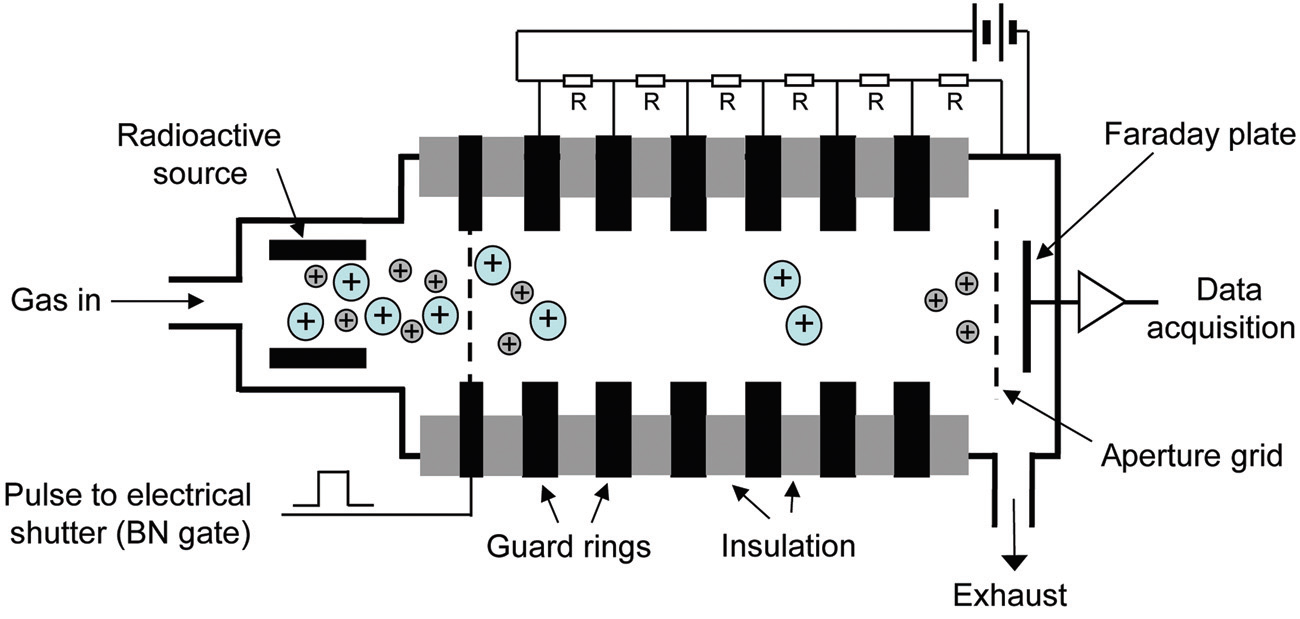
\includegraphics[width=0.65\linewidth]{pics/ims.png}
    \caption{Schematic diagram of an IMS instrument. Copyright \textcopyright  \citeauthor{ellis2013proton},  \citeyear{ellis2013proton}.}
    \label{fig:ims}
\end{figure}












\subsubsection{Selected Ion Flow Tube Mass Spectrometry}
Unlike IMS, selected ion flow tube mass spectrometry (\acrshort{sift}) does not use a drift tube, but a flow tube, to drag the ions downstream. As shown in \autoref{fig:sift}, a SIFT-MS instrument consist of an ion source, a quadrupole mass filter, a flow tube and a mass analyser.

The reagent ions (e.g. H$_3$O$^+$, NO$^+$ and O$_2^+$) are created in the ion source, which is typically a microwave resonator \cite{smith2005selected}.
Then, the quadrupole mass filter  selects the reagent ion by its mass. This piece of equipment also allows fast switching (tens of milliseconds) between the reagent ions, which can be used to extract more information of the analyte during transient experiments. From the quadrupole mass filter, the ions enter the flow tube. Here helium is used as a carrier gas and it is also in the flow tube where the analyte gas is injected. Finally, the ions are detected in a mass analyser, typically a quadrupole mass spectrometer, and the detection system builds the mass spectra obtained from the reaction of the reagent ions with the analyte.



The presence of helium in the flow tube makes it possible to explore ion-molecule reactions at thermal energies. One of the main applications of SIFT-MS is the ability to measure reaction coefficients. This has allowed SIFT-MS to become a valuable tool in areas like atmospheric and interstellar chemistry, and it has also been used as an analytical tool in other fields, being breath analysis the most remarkable one \cite{turner2006longitudinal}.

\begin{figure}%[h]
\centering
    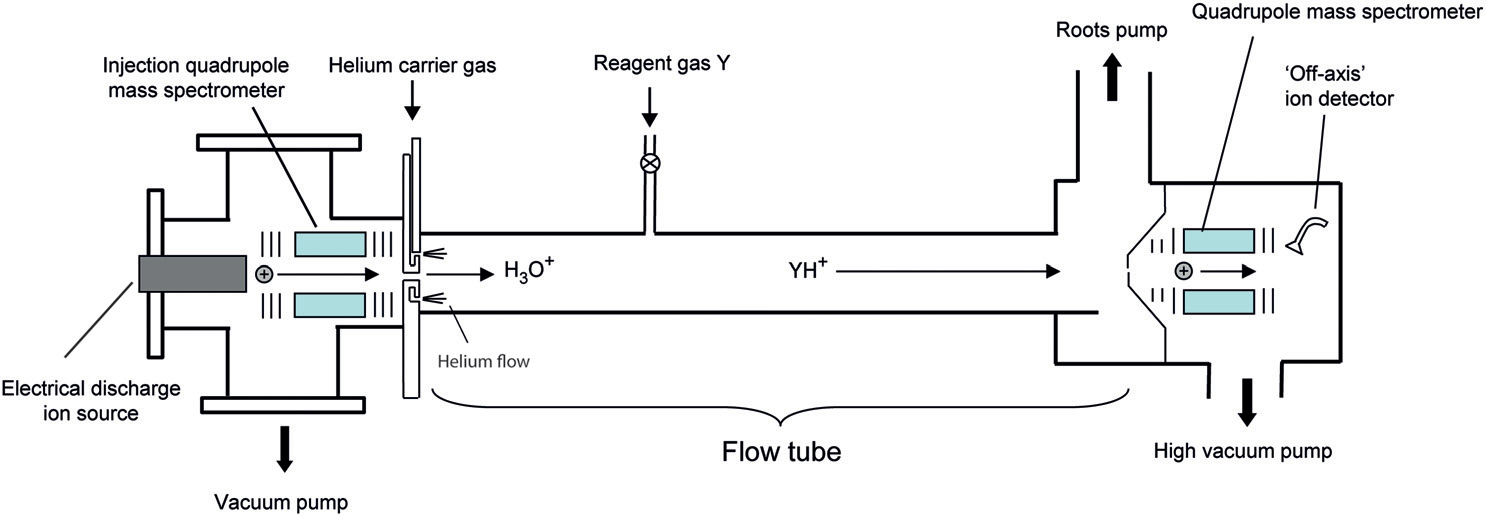
\includegraphics[width=0.95\linewidth]{pics/sift.png}
    \caption{Schematic diagram of a SIFT-MS instrument. Copyright \textcopyright  \citeauthor{ellis2013proton},  \citeyear{ellis2013proton}.}
    \label{fig:sift}
\end{figure}




\subsubsection{Proton Transfer Reaction Mass Spectrometry}
%\subsubsection{PTR-MS}
Proton transfer reaction mass spectrometry (\acrshort{ptrms}) is the main instrument used in the experimental work presented in this thesis.
It has both similarities and differences with both IMS and SIFT-MS techniques. This method was developed by Werner Lindinger at the University of Innsbruck (Austria) in the 1990 as the successor of the flowing afterglow  and the selected ion flow drift tube techniques \cite{RN601}.
The main components of a PTR-MS instrument are the ion source, the drift tube and the mass spectrometer.
Hydronium (and its water clusters) is generated in the ion source, typically a hollow cathode, from the water injected from the water reservoir. The reagent ions are then introduced into the drift tube (\acrshort{dt}). It is at this stage where they meet the analyte and proton transfer (and possible fragmentation) takes place, before the ions  are transferred then into the mass analyser, typically a time-of-flight or quadrupole mass spectrometer, for their detection. Further details of the working procedure of a PTR-MS instrument are given in the following chapter.

PTR-MS has many advantages, most of them also shared with other SCI-MS techniques. To begin with, it can detect a significant number of  VOCs such as aldehydes, ketones, aromatic compounds, alcohols,  nitriles and esters.
Because of its high sensitivity, PTR-MS can reach limits of detection of parts per quadrillion by volume (\acrshort{ppqv}) \cite{ioniconlod}.
Furthermore, reactions occurring close to the collisional rate and the possibility of directly sampling air allows for online, real-time operating conditions. Besides this, the only resources needed to run a PTR-MS instrument are distilled water and electric power.
Additionally, little or no fragmentation of the parent ions is observed, as compared to other ionisation mechanisms like EI. This  can however be manipulated to some extent by changing the conditions in the reactor. Also, selectivity can be enhanced by applying the recent instrumental developments which include, for instance, the development and implementation of an RF ion funnel \cite{barber2012increased,RF_TNT} and the use of a fast switching reduced electric field \cite{doi:10.1021/acs.analchem.7b05211}.

On the other hand, PTR-MS also has some disadvantages, being one of the most important ones the inability to directly distinguish between isomeric compounds, although this can be mitigated by using tandem MS$^n$ or fastGC techniques. % to enhance the selectivity.
Also, water cluster formation and detection can interfere with the detection of other molecules. For example, the $^{18}$O isotope of the first water cluster, (H$_2$O)H$_3$O$^+$, and the ion (C$_3$H$_3$)H$^+$ will  be both found at m/z 39. However, this issue can be solved with a high-resolution mass spectrometer and proper data analysis (e.g. using multi-peak fitting techniques or taking into account the isotopic distribution of the ions). Likewise, for compounds like benzene and toluene, which reach with H$_3$O$^+$ but not with (H$_2$O)H$_3$O$^+$, the sensitivity depends on the humidity of the air, because higher humidity means higher concentration of (H$_2$O)H$_3$O$^+$ and lower of H$_3$O$^+$. Finally, not all VOCs can be detected in PTR-MS. There exist some VOCs that don’t react with H$_3$O$^+$, like some alkanes, which have proton affinities below that of H$_2$O.












%\subsubsection{Applications of PTR-MS}
The ability of PTR-MS to detect and monitor trace concentrations of VOCs is advantageous in many fields. The main areas of application and some examples to illustrate them are:
atmospheric chemistry, where it has been used to study the emission of biogenic VOCs and their effect in the environment \cite{doi:10.1029/2003JD003863}, and to  monitor pollution and urban plumes \cite{ROGERS200626};
homeland security, where it has been  applied to  the detection of explosives \cite{RN445,RN1254,doi:10.1021/acs.analchem.7b05211}, rape drugs \cite{doi:10.1002/jms.2993}, and narcotics \cite{Agarwal2011};
in medical sciences, for the detection and monitoring of diseases through breath analysis \cite{FERNANDEZDELRIO20151243,doi:10.1152/jappl.2001.91.2.762,amann2014};
and in food sciences, to study  food aroma, flavour and quality control \cite{doi:10.1021/jf020922g,doi:10.1021/jf803998c,doi:10.1002/jms.1797}.















%\subsubsection{Advantages and disadvantages}
%Some of the advantages of most SCI-MS techniques, but in particular of PTR-MS, are:
%\begin{itemize}
%\item PTR-MS can detect a significant number of  VOCs such as aldehydes, ketones, aromatic compounds, alcohols,  nitriles and esters.
%\item Because of its high sensitivity, PTR-MS can reach limits of detection of parts per quadrillion by volume (\acrshort{ppqv}) can be achieved \cite{ioniconlod}.
%\item Little or no fragmentation of the ions, as compared to other ionisation mechanisms like electron impact.
%\item Real time measurement:
%\begin{itemize}
%\item Fast reactions, with a rate coefficient close to the collision rate, in the order of magnitude of 10$^{-9}$ cm$^{3}$/s.
%\item Direct sampling of atmospheric gases, which means that no sample preparation or pre-concentration is required.
%\end{itemize}
%\item Ease of operation, only requiring electrical power and distilled water.
%\item Sensitivity: latest instrumental developments allowed increase in sensitivity. For instance, the development and implementation of an RF ion funnel \cite{barber2012increased,RF_TNT} and the use of a fast switching reduced electric field \cite{doi:10.1021/acs.analchem.7b05211}.
%\end{itemize}

%On the other hand, PTR-MS also shows the following disadvantages:
%\begin{itemize}
%\item Inability to directly distinguish isomeric compounds. This can be mitigated by using tandem MS$^n$ or fastGC techniques to enhance the selectivity.

%\item Water cluster formation and detection can interfere with the detection of other molecules. For instance, the $^{18}$O isotope of the first water cluster, (H$_2$O)H$_3$O$^+$, and the ion (C$_3$H$_3$)H$^+$ will  be both found at m/z 39. However, this issue can be solved with a high-resolution mass spectrometer and proper data analysis, i.e. using multi-peak fitting techniques or taking into account the isotopic distribution of the ions.

%\item For compounds like benzene and toluene, which do not react with (H$_2$O)H$_3$O$^+$, the sensitivity depends on the humidity of the air, because higher humidity means higher concentration of (H$_2$O)H$_3$O$^+$ and lower of H$_3$O$^+$.

%\item There exist some VOCs that don’t react with H$_3$O$^+$, like some alkanes, which have proton affinities below that of H$_2$O, so the back reaction (equation \ref{eq:ptb}) is not negligible. %Isoflurane also has a lower proton affinity lower than that of water, but product ions are observed.
%\end{itemize}





%\begin{itemize}
%\item Atmospheric chemistry:
%\begin{itemize}
%\item Determination of the emission of biogenic VOCs and their effect in the environment \cite{doi:10.1029/2003JD003863}.
%\item Monitoring of pollution and urban plumes \cite{ROGERS200626}.
%\end{itemize}
%\item Homeland security:
%\begin{itemize}
%\item Detection of explosives \cite{RN445,RN1254,doi:10.1021/acs.analchem.7b05211}, rape drugs \cite{doi:10.1002/jms.2993} and narcotics \cite{Agarwal2011}.
%\end{itemize}
%\item Medical sciences:
%\begin{itemize}
%\item Detection and monitoring of diseases through breath analysis \cite{FERNANDEZDELRIO20151243,doi:10.1152/jappl.2001.91.2.762,amann2014}.
%\end{itemize}
%\item Food sciences:
%\begin{itemize}
%\item Study of food aroma and flavour and quality control cite{doi:10.1021/jf020922g,doi:10.1021/jf803998c,doi:10.1002/jms.1797}.
%\end{itemize}
%\end{itemize}





























\section{Thesis outline}
In the first chapter I present an introduction to soft chemical ionisation mass spectrometry together the outline  and the aim of the present thesis.

% 2 PTRMS

In the second chapter, the PTR-MS technique %, its underlying chemistry
and relevant experimental aspects are explained in detail.

% 3 cocaine
% 4 other drugs
The first chapter including experimental work is the third one, where cocaine and related compounds of interest are investigated, including results from both PTR-MS and density functional theory calculations.

The fourth chapter  carries on with the same topic, with PTR-MS results from the measurements of other illicit drugs of common societal abuse.

% 5 RF nitros
The fifth chapter is an adapted version of my  paper regarding the enhancement of selectivity in the detection of %nitro-, dinitro- and trinitrotoluenes
explosives
through the implementation of an RF ion funnel in the reactor of a PTR-ToF-MS.

% 6 nitroanilines
The sixth chapter is a reformatted version of my  paper about the use selective reagent ion mass spectrometry for the study of nitroanilines isomers.

% 7 phthalates
The seventh chapter is an adapted version of my  paper regarding the investigations of phthalates in PTR-MS using direct headspace sampling.

% 8 ketones
The eighth chapter is a rewritten version of my  paper of relevance to breath analysis about the study of ketones using a fastGC-PTR-ToF-MS instrument %at  different humidities.
in dry and humid conditions.

% 9 conclusions
In the ninth chapter the final conclusions and closing remarks are stated.

%In the appendices I include papers, other data that didn't fit in the thesis, etc



\section{Aim of the thesis}
My research project was focused on the study of ion-molecule interactions in the reaction region of proton transfer reaction mass spectrometry,  mainly in the area of homeland security, but other applications have also been investigated, including a study of ketones of relevance to breath analysis.

Compounds of specific interest for my research are  illicit drugs, explosives and phthalates. The available studies, if any, had been done at only one reduced electric field (typically between 120 – 140 Td). The experimental work in this thesis  is supplemented by quantum chemical calculations, which are used to help interpret the results. These were conducted using Gaussian09W and GaussView05 for Windows by Dr Peter Watts. All calculations used the B3LYP hybrid functional and the 6-31+G(d,p) basis set.

The main outcome of this thesis has strengthened knowledge of ion-molecule interactions in \acrshort{scims} techniques, in collaboration with other research groups and institutions within the Marie Sk\l{}odowska-Curie Actions Innovative Training Network IMPACT: Ion-Molecule Processes for Analytical Chemistry Technologies (\href{www.impact-h2020itn.com}{www.impact-h2020itn.com}) funded by the European Commission’s HORIZON 2020 Programme under Grant Agreement Number 674911.


%At least three publications are expected as first author as well as other publications from collaborations as second or third author.
%The planned secondments and trainings in other institutions have taken place.


% OLD

%\texttt{The topic of my thesis is the underpinning of ion-molecule processes and their use as analytical probes in soft chemical ionisation mass spectrometry (SCIMS). This includes studying specific ion-molecule reaction processes and their dependence on temperature, reduced electric field, pressure, etc. This is being done in the field of homeland security, in particular to illicit drugs. I am also interested in studying the implementation of a radio frequency ion funnel in PTR-MS to enhance selectivity and sensitivity, and the use of a thermal desorption unit as method to detect semi volatile organic compounds. Moreover, I want to use computational methods to study the trajectories of ions inside the reactor of a PTR-MS instrument at different experimental conditions to gain knowledge about the transmission of ions to the subsequent stages of a PTR-MS instrument. Furthermore, I am one of the ten early stage researchers (ESRs) of the IMPACT network (see appendix).}









\chapter{Proton Transfer Reaction Mass Spectrometry}\label{chapter:ptr}
\markboth{PTR-MS}{}

In this chapter, proton transfer reaction mass spectrometry, %(\acrshort{ptrms})
 its underlying chemistry and relevant experimental aspects
are explained.





\section{The PTR-ToF-MS}
As stated in the introduction, PTR-MS is a sensitive technique for real-time monitoring of VOCs in air with a minimal sample preparation. PTR-MS uses hydronium as reagent ion to donate protons to the VOCs present in the analyte gas and detect trace concentrations of targeted compounds.  The KORE Technology Ltd RFIF Mk I PTR-ToF-MS instrument in our laboratory is shown in \autoref{fig:littoral}. 
The main  parts of a PTR-MS instrument and their functions can be simplified to:
\begin{enumerate}
    \item Ion source: production of reagent ions.
    \item Drift tube: protonation and possible fragmentation of the analyte.
    \item Mass spectrometer: detection and identification of product ions.
\end{enumerate}
  These are explained in detail in the following sections.

\begin{figure}%[h]
\centering
\sidesubfloat[]{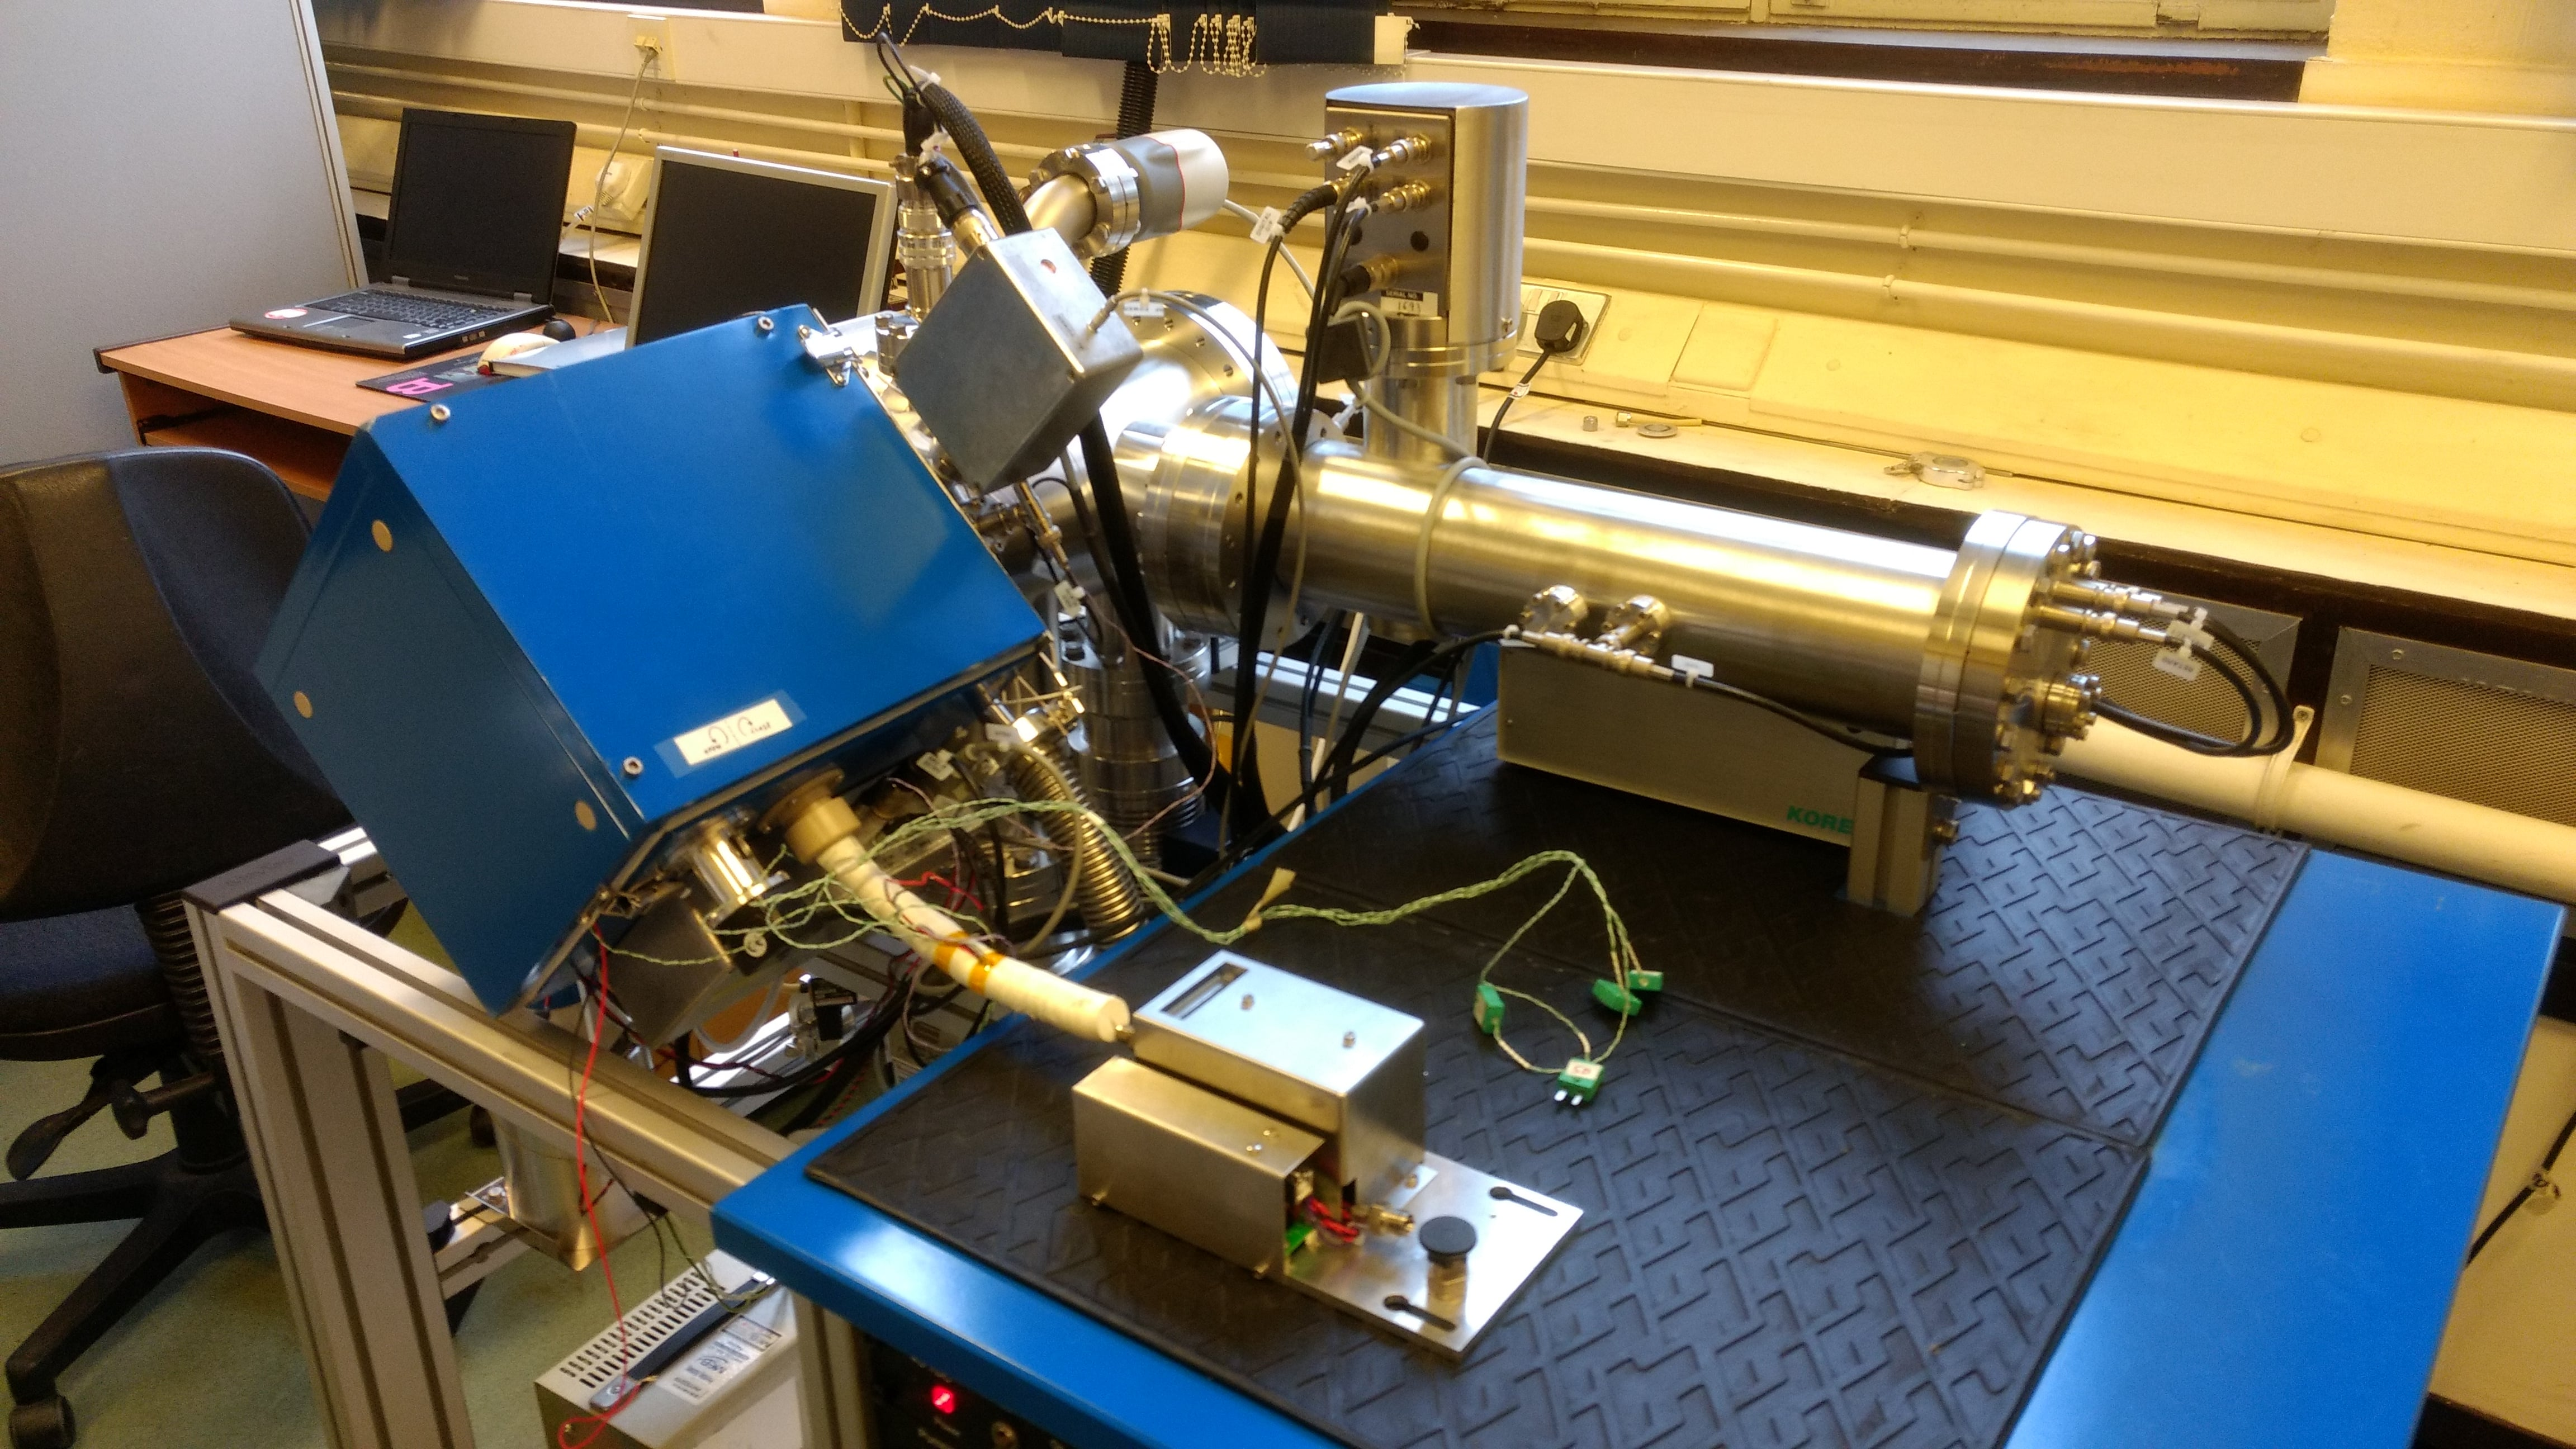
\includegraphics[width=0.9\linewidth]{pics/IMG_20170131_122756718.png}}

\bigskip
\sidesubfloat[]{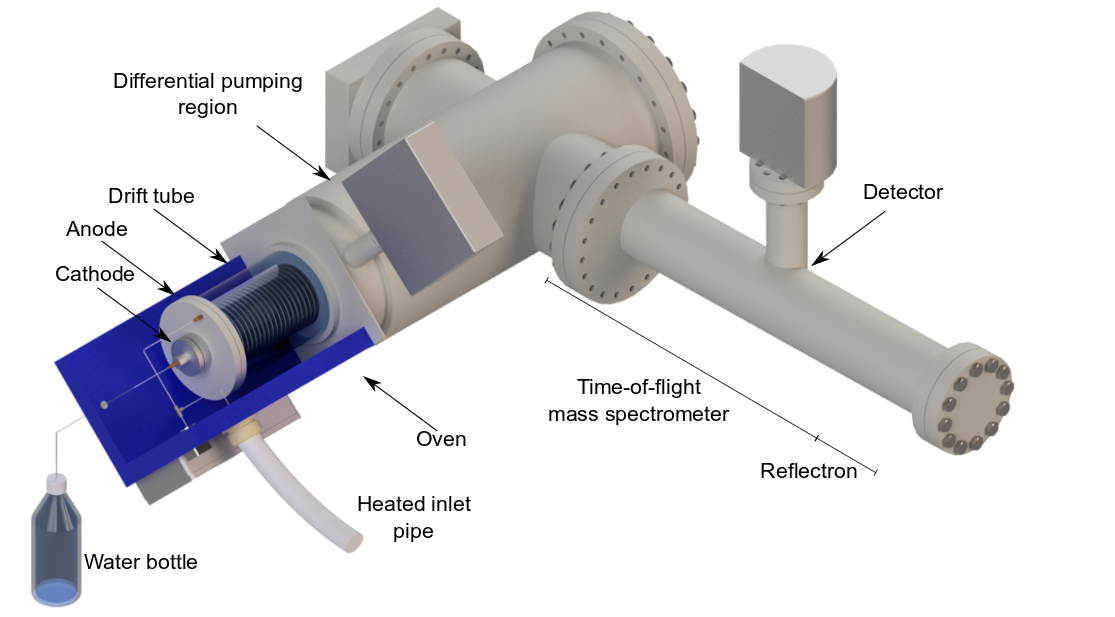
\includegraphics[width=0.95\linewidth]{pics/ptr-ilus.png}}
\caption{(a) Picture of the KORE Technology Ltd RFIF Mk I PTR-ToF-MS  with the TDU attached.  (b) Illustration of the same instrument (not to scale) including the naming convention.}
\label{fig:littoral}
\end{figure}




\subsection{Ion source}
The reagent ions that will ionise the sample are generated in the glow discharge (\acrshort{gd}) %that occurs
in the ion source. Most PTR-MS instruments carry a hollow cathode discharge ion source, to which a voltage is supplied to ionise the gas that flows through it and create the plasma in which the reagent ions are being produced.
%
The cathode in our PTR-MS instrument is shown in \autoref{fig:cathode},
although there are alternatives available like the triple off-axis cathode recently developed by \citeauthor{trion} that  allows to quickly switch from different reagent ion species
\cite{trion}.
%
Note that from now on I will indistinctly refer to plasma, discharge and glow discharge.



%The main advantage of a hollow cathode compared to a planar-electrodes ion source is that in the former higher ion densities can be achieved as the probability that ions hit the ion source's surface generating more ions is higher than in the planar electrode configuration.



\begin{figure}[t]
\centering
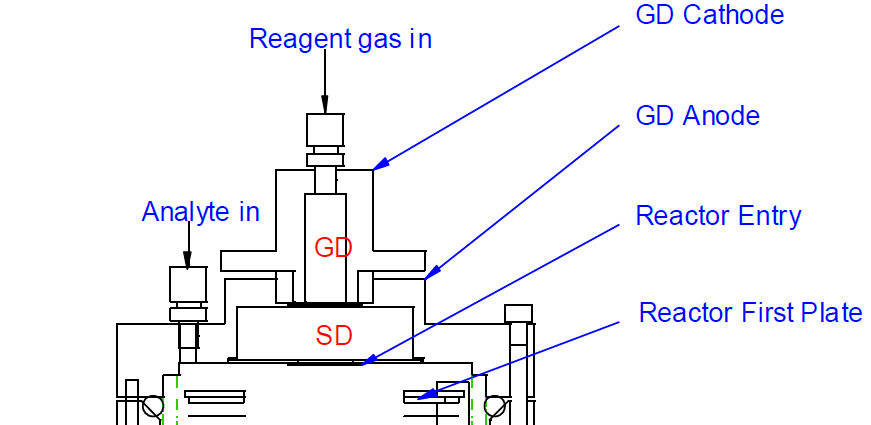
\includegraphics[width=0.6\linewidth]{pics/cathode.png}
\centering
\caption{Diagram of the hollow cathode of the PTR-MS apparatus manufactured by KORE Technology Ltd.}
\label{fig:cathode}
\end{figure}

%\subsubsection{Experimental aspects}







\subsubsection{The glow discharge: production of reagent ions}
Glow discharge is a type of electrical discharge that occur at low pressures (mbar range) and is characterised by a maintained current, ranging from 1uA to 1A, between the cathode and the anode. It receives this name because the ionised gas produces a shining glow whose characteristics depends on the nature of the gas, its pressure and the voltage applied.

During the standard use of the instrument, water vapour is supplied from the water reservoir through a needle valve to the cathode, where H$_3$O$^+$ ions are generated.
The main reaction occurring in the ion source leading to the production of H$_3$O$^+$ from the electrical discharge of water vapour is the first one shown in \autoref{tb:reactions}. It starts when H$_2$O$^+$ has been produced through the electron impact ionisation of water. However, other water fragment ions can also undergo reactions that generate hydronium, following the other reactions shown in \autoref{tb:reactions}. The rate  at which these reactions happen is very close to the collisional  rate.
Furthermore, hydronium ions can cluster to water molecules via hydrogen bonds to form the so-called water cluster ions, i.e. (H$_2$O)$_n$H$_3$O$^+$ with n = 1, 2, 3, ...
Ideally, the formation of these clusters should be avoided to inject pure hydronium into the drift tube.
Otherwise, if the water cluster ions come into play, there are  proton transfer reactions simultaneously occurring in the drift tube with different energies, which makes it more difficult to understand the energetics associated with the different protonation and fragmentation pathways.


The breakdown voltage, which is the voltage difference needed between cathode and anode to start the plasma, is of approximately 750 V for the cathode with the geometry described in \autoref{fig:cathode}.
%
However, after the plasma has started, the voltage difference to maintain the discharge goes down to approximately 350 - 400 V.
%
The anode voltage floats with the voltage of the first plate of the drift tube electrodes, which can be adjusted by the user to set the drift voltage, as will be discussed in the next section. After the glow discharge switch is turned on, it can take the plasma up to a couple of minutes to start.
%Increasing the pressure in the drift tube can assist to start the plasma, as some of the gas in the drift tube will be back-streamed into the cathode and O$_2$ requires a lower voltage to start a plasma.
In our instrument, the ion source pressure is usually between 1 and 1.4 mbar.
%If even with some back-streaming and setting the cathode at high pressure the plasma will not start, cleaning the ion source must be considered.
The plasma struggling to get started or maintained at a pressure  within the common operating range
indicates that the hollow cathode must be cleaned, as an aluminium oxide layer can form inside  and needs to be removed. Another factor that affects the stability of the glow is the temperature of the oven that contains the ion source and the drift tube: %It has been observed that 
the higher the temperature of the oven is, the higher the cathode pressure must be for the glow to be maintained.



%An example of anode and cathode voltages in this configuration would be an anode voltage of 450 volts and a cathode voltage of -300 volts.





\begin{table}[t]
\centering
\caption{Chemical reactions through which hydronium can be produced starting from products of EI of water vapour and their rate coefficients at 300K \cite{doi:10.1002/rcm.1290030312}.}
\label{tb:reactions}
\begin{tabular}{ rcl l }
\toprule
\quad H$_2$O$^+$ + H$_2$O 	&$\rightarrow$& H$_3$O$^+$ + OH  	& k = 1.8$\times$10$^{-9}$\, cm$^{3}$s$^{-1}$ \qquad \\ \midrule
OH$^+$ + H$_2$O  	&$\rightarrow$& H$_3$O$^+$ + O  		& k = 1.3$\times$10$^{-9}$\, cm$^{3}$s$^{-1}$  \\
				& $\rightarrow$& H$_3$O$^+$ + OH		& k = 1.8$\times$10$^{-9}$\, cm$^{3}$s$^{-1}$	  \\ \midrule
O$^+$ + H$_2$O  	&$\rightarrow$& H$_2$O$^+$ + O  		& k = 2.6$\times$10$^{-9}$\, cm$^{3}$s$^{-1}$   \\ \midrule
H$_2^+$ + H$_2$O  	&$\rightarrow$& H$_3$O$^+$ + H  		& k = 3.4$\times$10$^{-9}$\, cm$^{3}$s$^{-1}$   \\
				& $\rightarrow$& H$_2$O$^+$ + H$_2$ 		& k = 3.7$\times$10$^{-9}$\, cm$^{3}$s$^{-1}$	  \\ \midrule
H$^+$ + H$_2$O  	&$\rightarrow$& H$_2$O$^+$ + H  		& k = 8.2$\times$10$^{-9}$\, cm$^{3}$s$^{-1}$   \\ \bottomrule
\\
\end{tabular}
\end{table}



Downstream from the ion source, the ions reach the so-called source drift (\acrshort{sd}) region (shown in  \autoref{fig:cathode}), whose goal is to break the clusters apart before they enter the drift tube. If said clusters are not broken before entering the drift tube, they can also  split up there through collisions with the buffer gas.










\subsection{Drift tube}
The drift tube %(\acrshort{dt})
is the region of a PTR-MS instrument where the protonation and possible fragmentation of the analyte occurs. It is also often referred to as the reactor. A picture of the DT out of the front-end of the PTR-ToF-MS is shown in \autoref{fig:dt}.

\begin{figure}%[h]
\centering
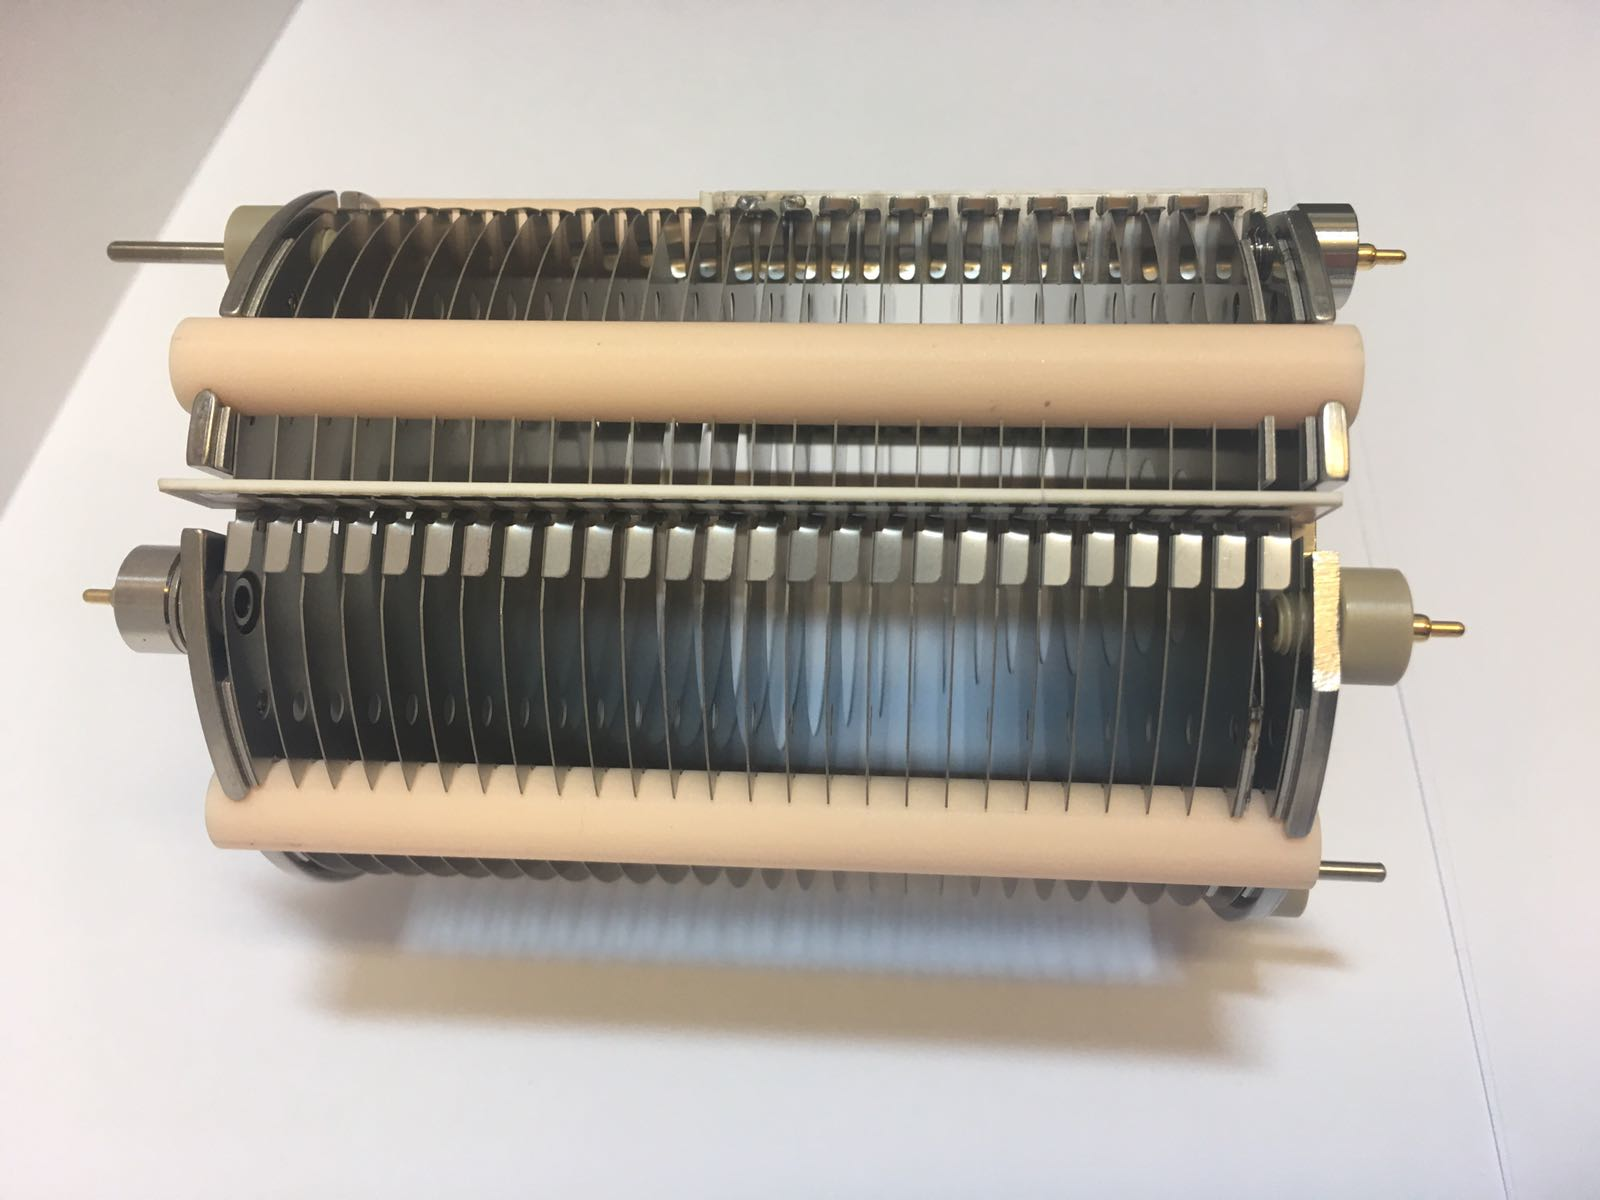
\includegraphics[width=0.6\linewidth]{pics/IMG-20170119-WA0008.png}
\centering
\caption[Picture of the drift tube.]{Picture of the drift tube. Note that in this model the diameter of the electrodes steadily decreases in the second half of the stack.}
\label{fig:dt}
\end{figure}


%\subsubsection{Experimental details}

The drift tube of the KORE Technology Ltd RFIF Series 1 PTR-ToF-MS, whose schematic layout is shown in \autoref{fig:dt_diagram}, consists of 29 stainless-steel ring electrodes of 0.2 mm of thickness with a spacing of 3.2 mm per plate inside a cylinder of resistive glass.
The inner diameter of these electrodes is 40 mm in the first half of the stack and it gradually decreases in the second half to 6 mm.
A 1 M$\Omega$ resistor chain connected to the electrodes allows to supply a linearly decreasing potential to each of them when a voltage is applied between the first and the last plates, generating an electric field in the reactor known as DC field.
When the instrument is operating in these conditions (i.e. without the RF field explained later in \autoref{section:rfif}), we refer to it as working in DC mode or DC-only mode.
% this is repeated in the RF paper

\begin{figure}[t]
\centering
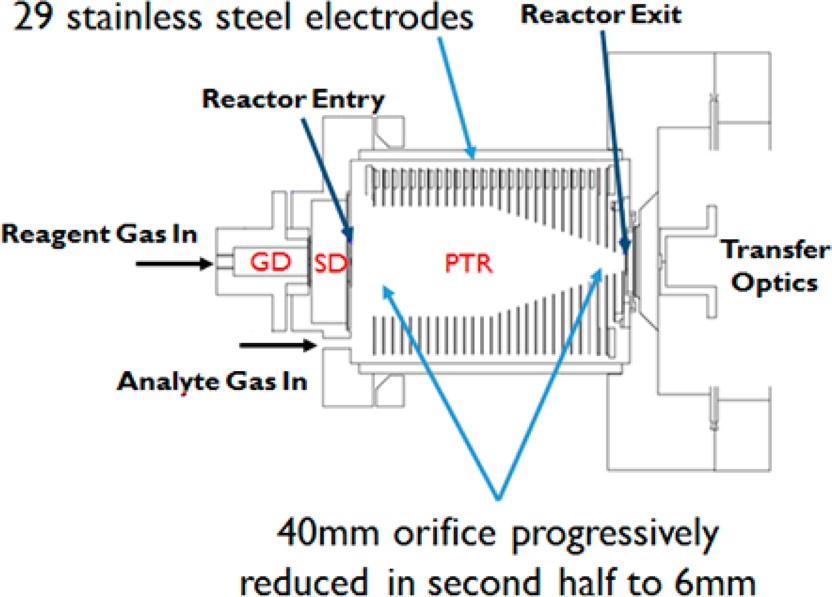
\includegraphics[width=0.6\linewidth]{pics/ac-2016-02982x_0002.png}
\centering
\caption{Schematic diagram of the KORE Technology Ltd RFIF Series 1 PTR-ToF-MS drift tube, together with the glow discharge and the source drift.}
\label{fig:dt_diagram}
\end{figure}

The DC electric field (see \autoref{fig:dt_simion}) drags the ions across the reactor and towards the transfer lenses, where they will get transmitted into the mass spectrometer. As they are drawn through the reactor, ions collide with the neutrals molecules of the background and analyte gases, which can result in protonation and fragmentation of the analyte. The collisional energy can be manipulated by tuning the DC field as well as the reactor's pressure and temperature, whose standard operating values are around 1 mbar and between 100 and 150$^{\circ}$C, respectively, although our oven can reach up to 200$^{\circ}$C.




\begin{figure}[t]
\centering
\sidesubfloat[]{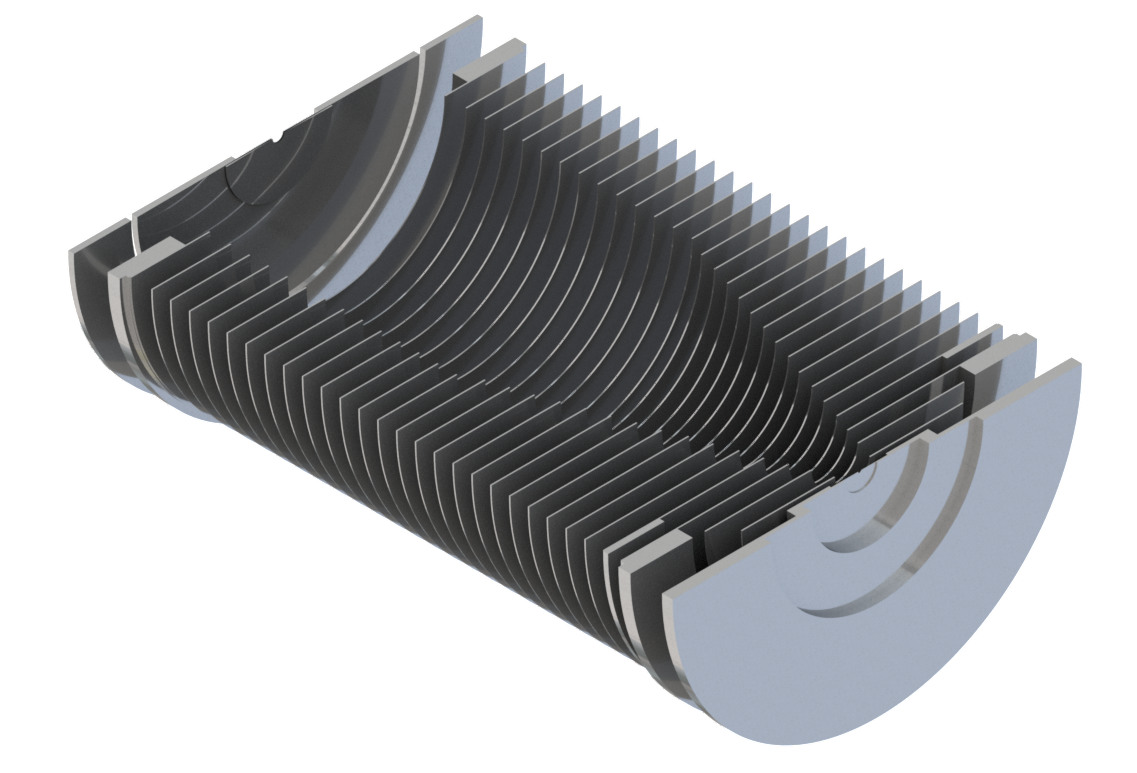
\includegraphics[width=0.4\linewidth]{pics/rfreactorm4.png}}
\sidesubfloat[]{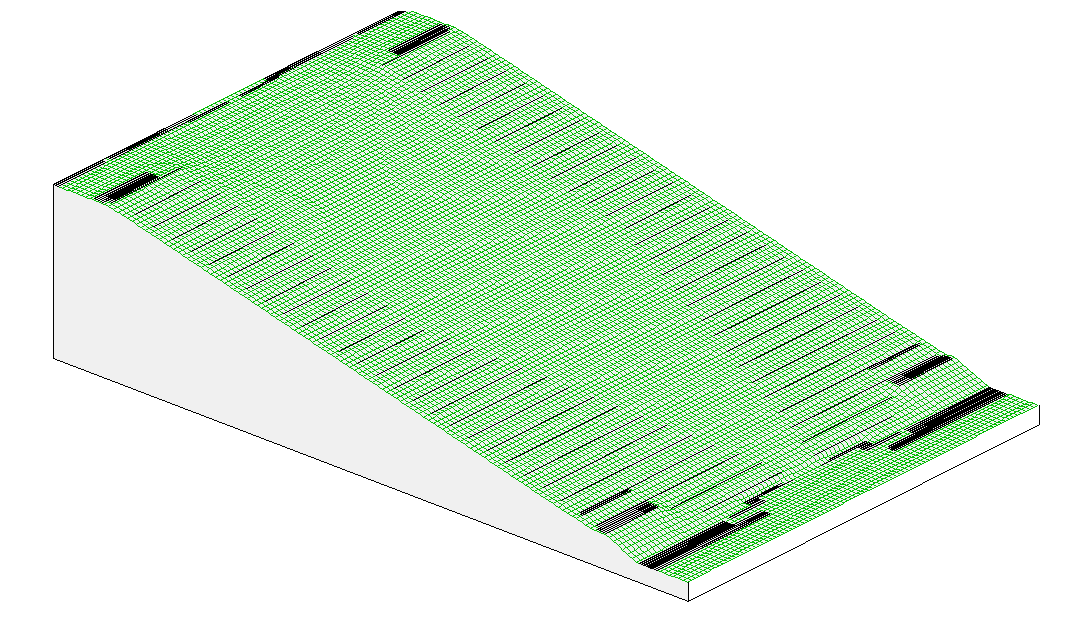
\includegraphics[width=0.4\linewidth]{pics/DC_SIMION.png}}
\centering
\caption{(a) Half section view of the reactor. (b) Potential energy surface of the cross section of the reactor in DC mode calculated in SIMION\textsuperscript{\textregistered} for a random drift voltage.}
\label{fig:dt_simion}
\end{figure}




\subsubsection{Reduced electric field}
As the collisional energy depends not only on the electric field strength (\acrshort{e}) but also on the buffer gas in the reactor, it is convenient to use the reduced electric field (\textit{\acrshort{en}}) as a measure of the collisional energy delivered to the ions.
First, the electric field strength  is defined by the potential difference between the first and the last plate in the reactor divided by its length (\autoref{eq:E}):
\begin{equation}
E = \frac{V_d}{L}
\label{eq:E}
\end{equation}
where \acrshort{Vd} is the so-called drift voltage and it is equal to the voltage difference between the first and the last plate of the reactor, known as PTR Entry and PTR Exit voltages,
that can be adjusted by the user, and L is the length of the drift tube, which is 9.36 cm in our newest instrument.
For instance, a voltage difference between first and last plates of 250 V corresponds to an electric field of 26.71 V/cm.

Similarly, the gas number density (\acrshort{n})  is defined as the number of gas particles per unit volume and can be calculated from the ideal gas equation to be (\autoref{eq:N}):
\begin{equation}
N = \frac{N_A}{V_{mol}}\frac{P_d}{P_0}\frac{T_0}{T_d}
\label{eq:N}
\end{equation}
where \acrshort{na} is the Avogadro's number (6.022$\times$10$^{23}$ mol$^{-1}$), V$_{mol}$ (22414 cm$^{3}$ mol$^{-1}$) is the molar volume of an ideal gas at standard temperature and pressure conditions \acrshort{p0}  and \acrshort{t0}, T$_d$ is the temperature of the drift tube in Kelvin and P$_d$ is the gas pressure in the drift tube in mbar.
For the standard operations conditions of 1 mbar and 100$^{\circ}$C, N is 1.94$\times$10$^{16}$ cm$^{-3}$.
The ratio \textit{E/N} in this case would be 26.71 V cm$^{-1}$/1.94$\times$10$^{16}$ cm$^{-3}$ $\simeq$ 1.38$\times$10$^{-15}$ V cm$^{2}$.
However, it is usual to express the reduced electric field in a different unit called Townsend (\acrshort{td}), which corresponds to 10$^{-17}$ V cm$^{2}$.
Thus, 1.38$\times$10$^{-15}$ V cm$^{2}$ corresponds to a value of 138 Td.
Typically, a PTR-MS instrument is operated between 120 and 140 Td but going as low as 80 Td or as high as 240 Td is sometimes crucial to get a good picture of the dependence of the ion-molecule reactions with the collisional energy.

The ions inside the reactor reach a steady velocity, the so-called drift velocity, \acrshort{vd}, which is proportional to the electric field (\autoref{eq:vd}):
\begin{equation}
v_d = K\cdot E
\label{eq:vd}
\end{equation}
where \acrshort{kk} is the ion mobility, which depends on the ion's mass and structure, and the temperature and pressure in the drift tube, and E the electric field strength.
Note that the product of the ion mobility and the electric field must not be mistaken with the kinetic energy, often referred to as KE.
Also note that the drift velocity does not represent the velocity of an individual ion but an average over the ion cloud, and it can be also  expressed in terms of the reduced mobility, \acrshort{kk0}, and the gas number density at standard pressure and temperature, \acrshort{n0}:
\begin{equation}
v_d = K_0 N_0 \frac{E}{N}
\label{eq:vd2}
\end{equation}
% where K and N are related to K$_0$ and N$_0$ through  \autoref{eq:k0} and \autoref{eq:n0}:

% \begin{equation}
% N = \frac{P_d}{P_0}\frac{T_0}{T_d}N_0			%I am not sure about this equation
% \label{eq:n0}
% \end{equation}

Moreover, the expression for the total mean kinetic  energy of an ion, including both the thermal energy and the energy coming from the electric field, was formulated by \citeauthor{wannier1951bell} \cite{wannier1951bell,wannier1952motion}: % (\autoref{eq:KEions}):
\begin{equation}
    \label{eq:KEions}
    KE_{ion} = \frac{3}{2}k_B T + \frac{1}{2}m_{ion} v_d^2 + \frac{1}{2}m_b v_d^2
\end{equation}
The first term represents the contribution of the thermal energy to the ion's kinetic energy, with k$_B$ the Boltzmann constant and T  the drift tube temperature.
The second term relates to the kinetic energy of the ion from being dragged by the electric field at a drift velocity v$_d$, with m$_{ion}$ the mass of the ion.
Finally, \citeauthor{wannier1951bell} added the last term as the contribution to the ion's kinetic energy  from the randomly-oriented velocity of the ions coming from collisions between the ions and the buffer gas molecules of mass m$_b$, which would be 28.0 or 28.8 g/mol, depending on if N$_2$ or lab air is used as buffer gas.
%
This last term can be used to describe an ``effective temperature'' T$_{eff}$ of the ions according to 
\citeauthor{revercomb1975theory} (\autoref{eq:teff})
\cite{revercomb1975theory}.
%
An estimated drift velocity of 900 m/s at 120 Td and a drift tube temperature of 100$^{\circ}$C yields T$_{eff}$ $\simeq$ 1280 K (i.e. approximately 1000$^{\circ}$C).
%
Whilst this looks like a huge increase in temperature, the ion’s kinetic energy is still way higher.
%
For an ion of \textit{m/z} 100 colliding with N$_2$ buffer gas molecules at 120 Td, the mean kinetic energy would be 0.58 eV, with the contribution from $(3/2)k_{B}T_{eff}$  only being 0.17 eV (i.e. around 29\% of the mean kinetic energy).
%
\begin{equation}
    T_{eff} = T\left(1 + \frac{m_b v_d^2}{3 k_B T}\right)
    \label{eq:teff}
\end{equation}


To properly characterise the energy involved in an ion-molecule collision, the relative energy of the participating bodies must be used instead of the total kinetic energy. This is given by the
%Because the \acrshort{en} is not unambiguously defined, ie different values of P, T and  V$_d$ can yield the same \acrshort{en}.
%Besides the reduced electric field,
the kinetic energy of the collision %of the ion and neutral (analyte)
in the centre-of-mass frame of reference, %\acrshort{kecm} (\autoref{eq:cm}) 
\cite{mcfarland1973flow}:
\begin{equation}
\label{eq:cm}
KE_{CM} = \frac{1}{2}\mu (v_{ion}^2 + v_n^2)
\end{equation}
where µ is the reduced mass of the 2-body system %(\autoref{eq:reduced_mass})%, and v$_{ion}$ and v$_n$ are the ion and neutral velocities, respectively.
\begin{equation}
\label{eq:reduced_mass}
\frac{1}{\mu} = \frac{1}{m_{ion}} + \frac{1}{m_{n}}
\end{equation}
and the kinetic energy of the ion and the neutral are defined by \autoref{eq:KEion2} and \autoref{eq:KT}, respectively:
\begin{equation}
\label{eq:KEion2}
KE_{ion} = \frac{1}{2}m_{ion}v_{ion}^2
\end{equation}

\begin{equation}
\label{eq:KT}
\frac{3}{2}k_B T = \frac{1}{2}m_{n}v_{n}^2
\end{equation}

Combining the expressions above, KE\textsubscript{CM} can be expressed as well as shown in \autoref{eq:cm_final}.
\begin{equation}
\label{eq:cm_final}
KE_{CM} = \frac{m_n}{m_n + m_{ion}} \left( \frac{m_{ion}v_d^2}{2} + \frac{m_{b}v_d^2}{2}\right) + \frac{3}{2}k_BT
\end{equation}
%
where the sub-index $n$ refers to the neutral molecule in both an ion-buffer gas collision or an ion-analyte collision, where only proton or charge transfer will occur in the latter case.
The difference between m$_n$ and m$_b$ for an ion-buffer gas collision is that m$_b$ is an average of the masses of the different species in the buffer gas, while m$_n$ is the mass of the species the ion is colliding with in each collision (e.g. N$_2$ or O$_2$ for lab air, if the rest of the constituents of air are neglected).
It is also important to bear in mind that v$_d$ and v$_{ion}$ are not necessarily the same, as v$_{ion}$ refers not only to the field-aligned velocity.
Note that, as v$_d$ is proportional to the \textit{E/N}, the KE\textsubscript{CM} is quadratic with the \textit{E/N}, as shown in \autoref{fig:KE} for cocaine and 2-butanone, which are two analyte molecules with a considerable mass difference and both are mentioned in this thesis. Their mass difference results in more energetic collisions (10 - 15\%) for cocaine than for 2-butanone.





% I plot these two because there is a big difference in mass and they are mentioned in the thesis.
\begin{figure}[t]
\centering
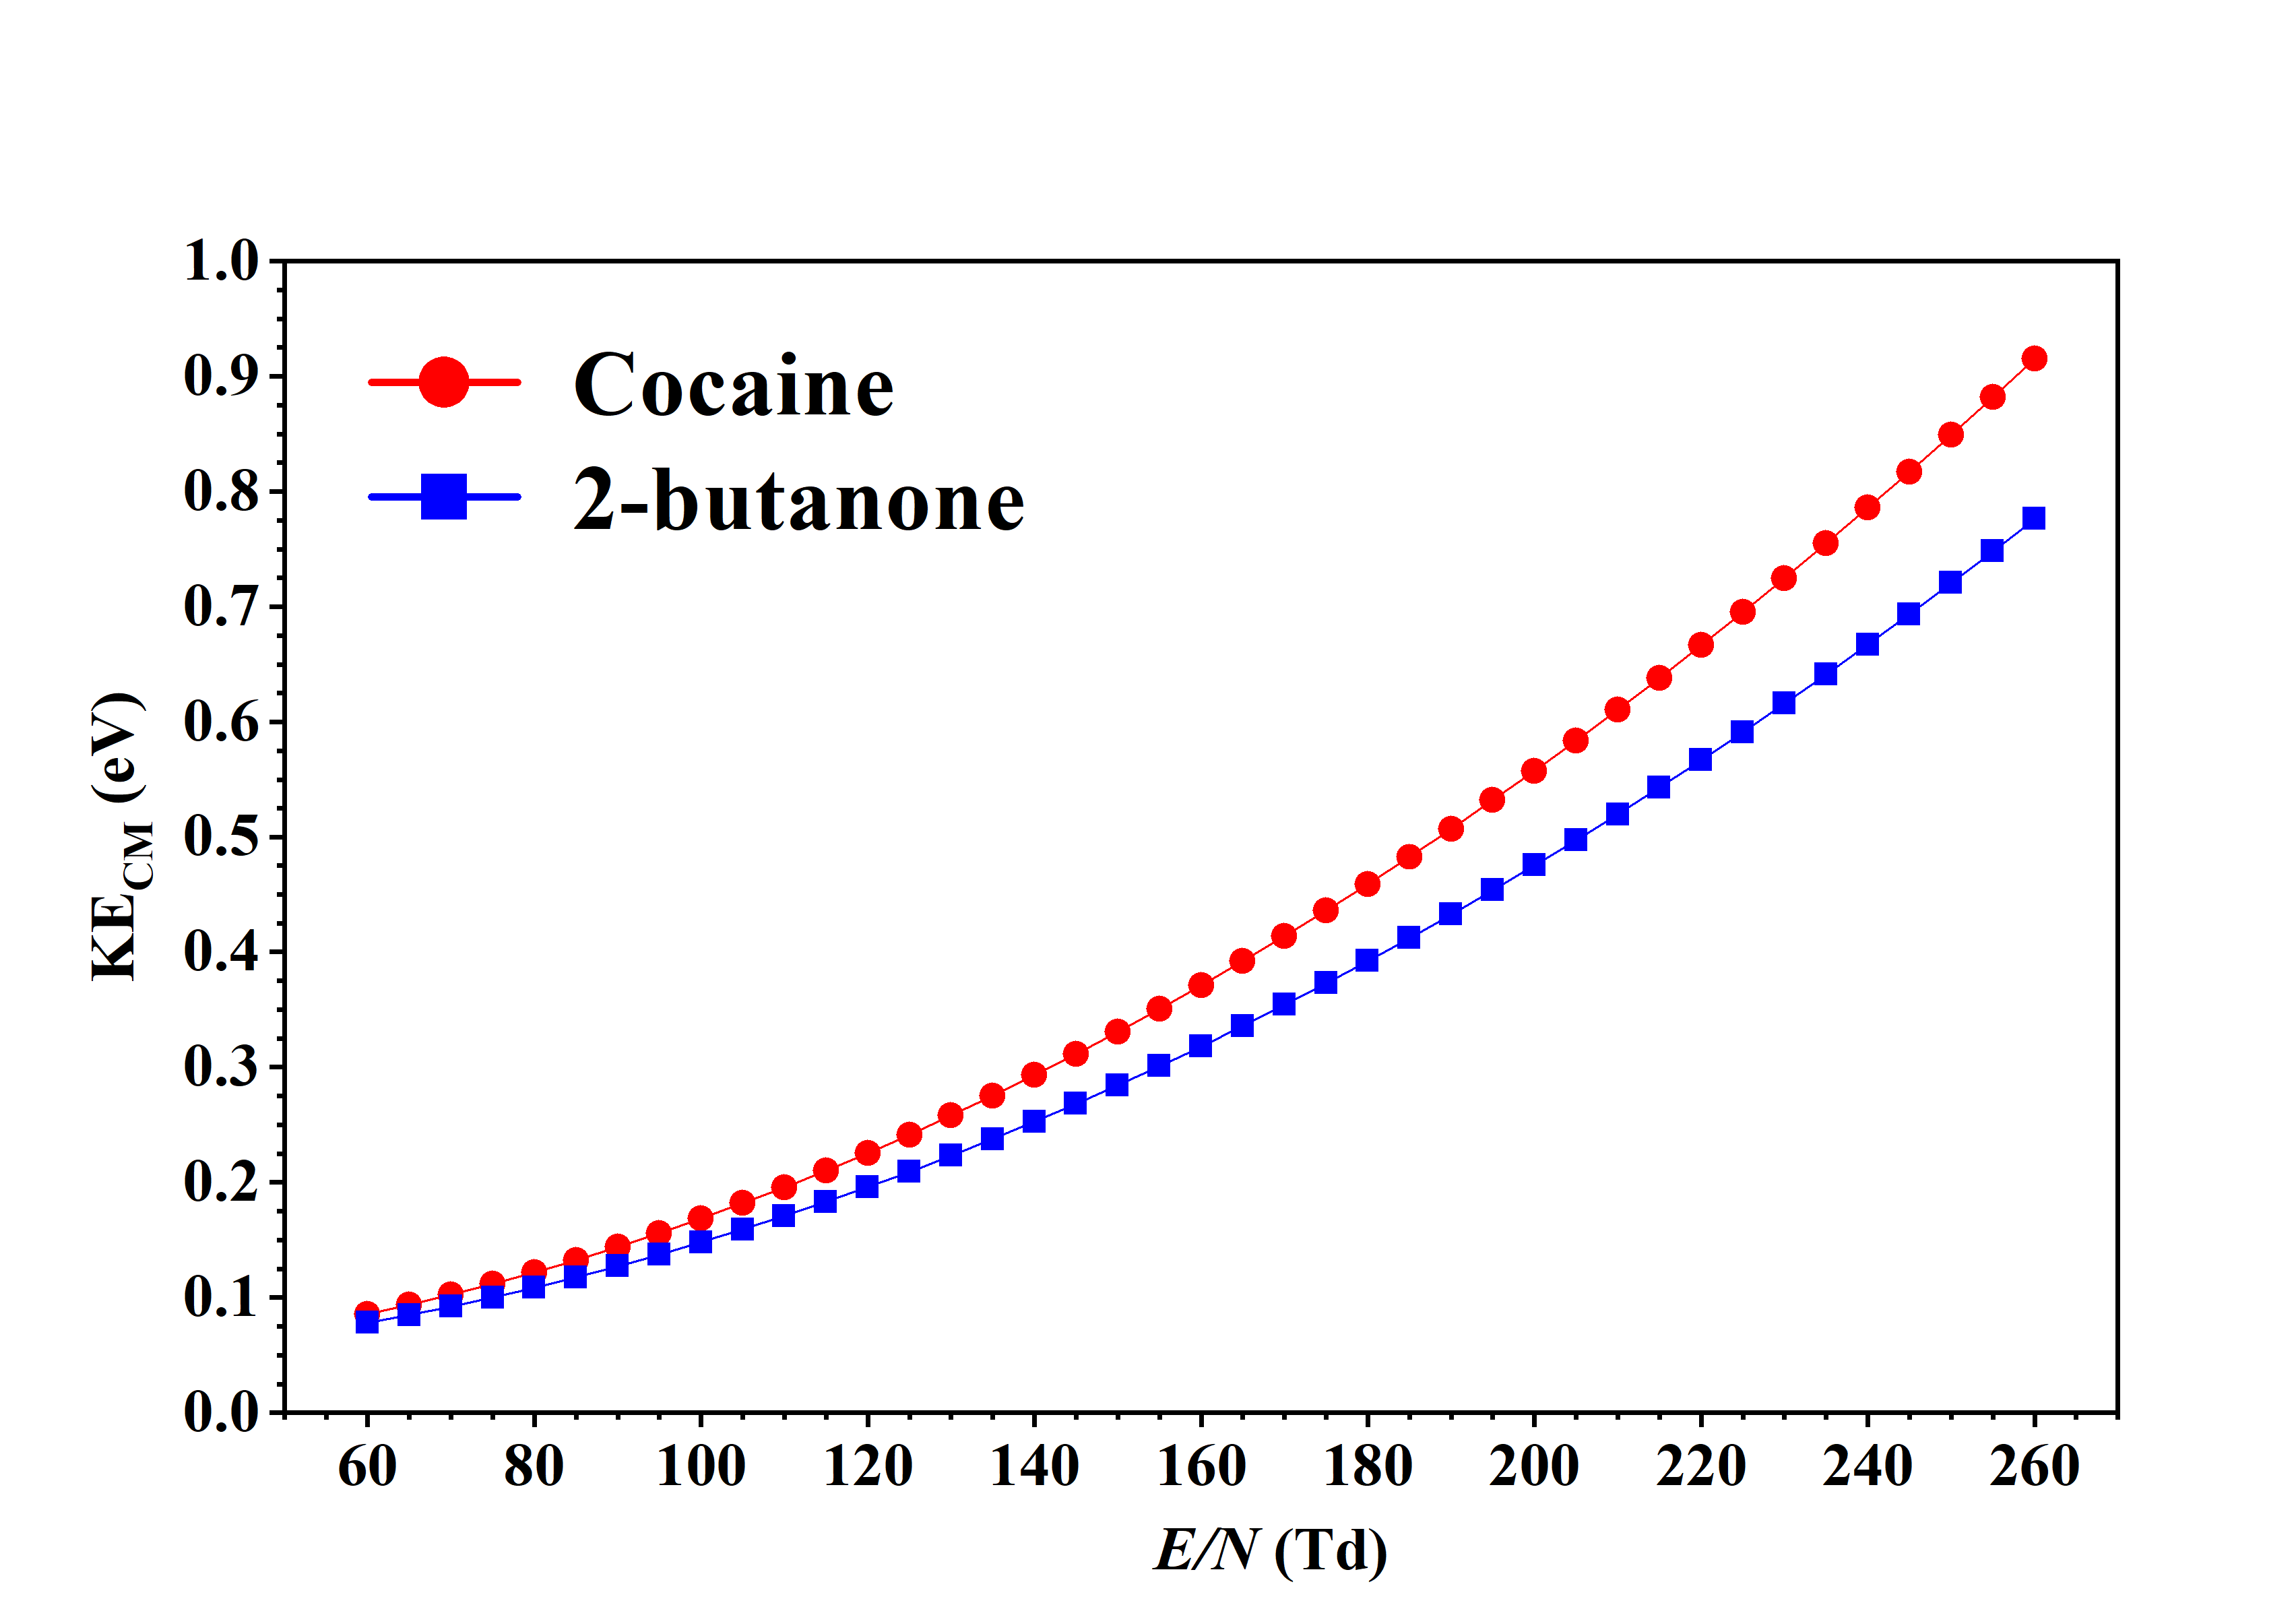
\includegraphics[width=0.7\linewidth]{pics/KE.png}
\centering
\caption{Plot of the kinetic energy of the collision
in the centre-of-mass frame of reference, KE\textsubscript{CM}, as a function of the \textit{E/N} for
collisions of H$_3$O$^+$ with cocaine (C$_{17}$H$_{21}$NO$_4$, 303 g/mol) or 2-butanone (C$_4$H$_8$O, 71 g/mol) at 300 K with N$_2$ as buffer gas. The values for K$_0$ and N$_0$ are  2.8 cm$^2$V$^{-1}$s$^{-1}$ and 2.69$\times$10$^{19}$ cm$^{-3}$, respectively.}
\label{fig:KE}
\end{figure}

















Contrary to the reduced electric field, the centre-of-mass kinetic energy is mass-dependent. %and depends on the ions mobility through their drift velocity.
The centre-of-mass is used rather than the lab reference frame as proton transfer reactions involve inelastic collisions because there is a transference of mass, but still in the centre-of-mass reference frame the sum of the linear momentum of each of the molecules is equal to zero both before and after the collision. % (\autoref{eq:cm2}).
%
%\begin{equation}
%\label{eq:cm2}
%\sum_i \vec{p}_{i,CM} = 0
%\end{equation}
%
Furthermore, the main challenge and source of error when using \autoref{eq:cm_final} is to measure the drift velocity accurately enough. This can be estimated from the ion mobility (\autoref{eq:vd2}) or using the Hadamard transformation \cite{doi:10.1002/rcm.7254}.






Ions will predominantly collide with  buffer gas molecules. \autoref{eq:mfp} gives the expression for the kinetic mean free path (\acrshort{mfp}, $\lambda$) defined as the average distance travelled between collisions, if the colliding particles are considered hard-spheres \cite{hirschfelder1954molecular}.
%
\begin{equation}
    \lambda = \frac{1}{\sqrt{2}N\pi d^2}
\label{eq:mfp}
\end{equation}
%
With d, the so-called kinetic diameter, being  3.64$\times$10$^{-10}$ m for N$_2$ and N = 2.41$\times$10$^{22}$ m$^{-3}$ at 1 mbar and 300 K 
the mean free path is of around 70 µm in the reactor, which corresponds to a viscous flow \cite{ismail2015gas}.
%
This can be compared to the regime in the mass spectrometer, where the pressure is around 10$^{-8}$ mbar and N $\simeq$ 10$^{15}$ m$^{-3}$: the mean free path grows up to the km order of magnitude, becoming much bigger than the dimensions of the chamber. In this case the flow is molecular and the predominant collisions are no longer with other particles but with the walls of the chamber.
%
The transition from the viscous to the molecular regime occurs in the differential pumping region.









%With this estimation, if the length of the drift tube is 9.36 cm, each ion will undergo around 1300 collisions on its way downstream the drift tube.
%However, note that this approximation does not depend on the residence time (or drift time) of the ion in the drift tube as it only accounts for the thermal contribution to the number of collisions.

%It is better to use the collision frequency, knowing that the thermal speed is........
%and hence the collision frequency is....


%knowing that the drift time for a H$_3$O$^+$ ion at 80 Td is approximately 150 µs and at 200 Td it is 70 µs.



%and its drift velocity approximately 900 m/s.

%Also, frequency of collisions.

%Do calculation of collisions per second.
















\subsubsection{Radio frequency ion funnel}\label{section:rfif}
The Radio Frequency Ion Funnel (\acrshort{rfif}) in the reactor of our instrument is a novel piece of equipment %developed by KORE Technology Ltd 
that both delivers extra collisional energy and focuses the ions towards the exit aperture of the drift tube, enhancing both sensitivity and selectivity of the PTR-MS instrument \cite{RF_TNT,barber2012increased}.

\begin{figure}[t]
\centering
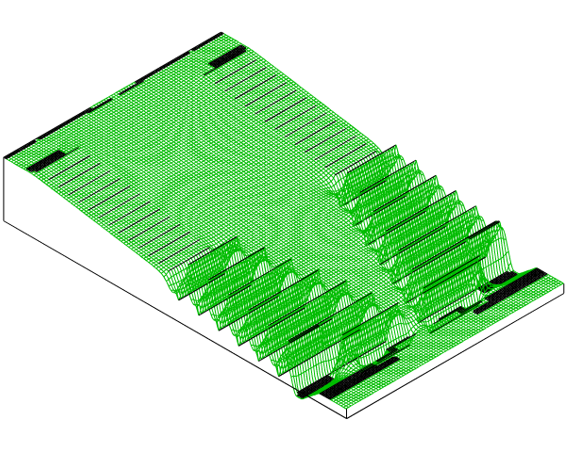
\includegraphics[width=0.6\linewidth]{pics/RF_SIMION.png}
\caption[Potential energy view of the cross section of the reactor in RF mode modelled in SIMION\textsuperscript{\textregistered} with a random DC field.]{Potential energy view of the cross section of the reactor in RF mode modelled in SIMION\textsuperscript{\textregistered} with a random DC field. Contrary to \autoref{fig:dt_simion}, this is a snapshot as the RF field is time-dependent.}
\label{fig:rfif_simion}
\end{figure}
%
%
As mentioned  earlier, in the second half of the drift tube stack the electrode's diameter gradually decreases from 40 mm to 6 mm in a funnel-like configuration. The suitable electronics to provide these funnel electrodes with an RF field are mounted in the instrument. These electronics
%consist of a RLC circuit that
provide the second half of the drift tube's electrodes with a signal of approximately 760 kHz and 200 V peak-to-peak in resonance that we will refer to as RF field (see \autoref{fig:rfif_simion}). At any given time, adjacent funnel plates are supplied with an RF field of opposite polarity. Also, this RF field can be turned on and off in the front panel of the instrument and when it is superimposed to the DC field, which is always on, the instrument is referred to as being operating in RF mode.
%It is also key to properly tune the capacitance from plate 29 to avoid ``closing'' the funnel.
Furthermore, in RF mode the reduced electric field, \textit{E/N}, cannot be used to refer to the collisional energy as in this mode the electric field  in the drift tube is no longer uniform. A comparison of the ion trajectories  in the second half of the drift tube in DC and RF modes is shown in \autoref{fig:rfif_vs_dc} for ions of \textit{m/z} 19 at a drift voltage of 200 V, which corresponds to around 120 Td in DC mode. The funnel effect can be observed on \autoref{fig:rfif_vs_dc}(b), which reveals a higher ion density near the exit of the reactor than that in DC mode, even though fewer ions were flown in the RF mode simulations %to reduce simulation times 
because this mode is computationally more demanding than DC mode.
%
\begin{figure}[t]
\centering
\sidesubfloat[]{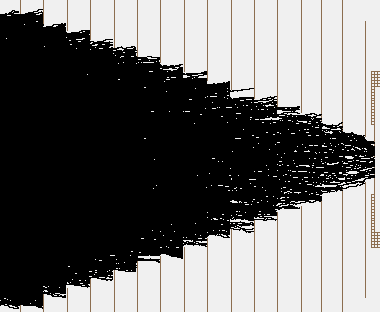
\includegraphics[height=0.23\textheight]{pics/DC_simulation_200V_120Td.png}}
\sidesubfloat[]{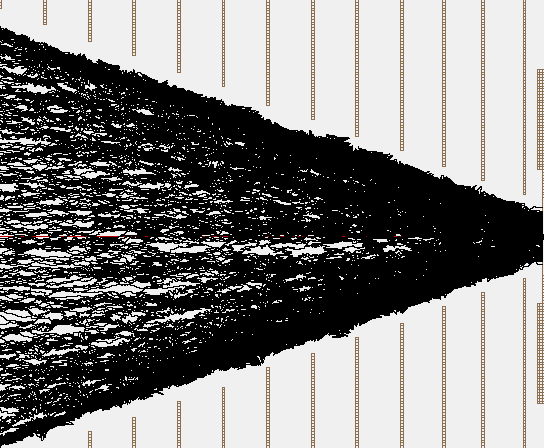
\includegraphics[height=0.23\textheight]{pics/ionfunnel3.png}}
\caption{Simulation of ion trajectories in (a) DC mode and (b) RF mode in the second half of the drift tube for ions of \textit{m/z} 19 at a drift voltage of 200 V (ca. 120 Td in DC mode).}
\label{fig:rfif_vs_dc}
\end{figure}


The ion funnel configuration described in this section is not the only one used in PTR-MS.
%
Others include a short, funnel-like stack of electrodes at the end of the drift tube
%\cite{piel2019airborne}
or 
use a quadrupole enveloping the drift tube
%a resistive glass drift tube that generates a more uniform electric field than the traditional electrode stack, to which an RF field is superimposed from 
\cite{piel2019airborne,krechmer2018evaluation}.



%Besides this design from KORE Technology Ltd, there are other  configurations available in the market.
%For instance, the reactor of IONICON Analytik GmbH instruments can include the so-called \textit{ION BOOSTER}, which is a short, funnel-like stack of electrodes at the end of the drift tube \cite{ionbooster}.
%On the other hand, the approach from TOFWERK consists of a resistive glass drift tube that generates a more uniform electric field than the traditional electrode stack, to which an RF field is superimposed from a quadrupole enveloping said drift tube \cite{krechmer2018evaluation}.


\subsubsection{Fast reduced electric field  switching}\label{section:fs}
Besides the \acrshort{rfif}, another one of the recent hardware developments %from KORE Technology Ltd, this time in conjunction with the \acrfull{dstl}, 
is the fast reduced electric field switching, or just fast switching.
%
It consists of a programmable 500 V power supply unit that can quickly switch the PTR Entry voltage between two preselected values in the range from 50 V to 450 V, which corresponds  to roughly the interval from 10 Td to 250 Td, at a chosen frequency.  This unit can be retrofitted into any other PTR-ToF-MS  from the same manufacturer.
This development has been applied to the detection of different explosives by \citeauthor{doi:10.1021/acs.analchem.7b05211} \cite{doi:10.1021/acs.analchem.7b05211}.
%demonstrated applicable to the detection of explosives %by \citeauthor{doi:10.1021/acs.analchem.7b05211}


A previous \textit{E/N} study of the molecule is needed to identify  the characteristic product ions beforehand. Then the two relevant PTR Entry voltage (i.e. \textit{E/N}) values and the switching frequency are selected.
The lower limit of the switching frequency, while still achieving optimal analytical results, is around 1 Hz.
This limit is a consequence of the time the reactor takes to clear out from product ions at a given reduced electric field, the so-called ``capacitance'', which is typically of around 150 - 200 ms.
The rise and fall times of the voltages given by the power supply unit are not symmetrical, but as these are tens of milliseconds, they get masked out by the capacitance.
%The data obtained  this way is stored in a .lst file
A temporal resolution of 25 ms has been found to be the optimum value %give the best results 
and  also proper data analysis is needed in order to discard the data acquired during the voltage changes.
This is done by means of a script %I wrote in Matlab\textsuperscript{\textregistered}, which is 
described in detail in  section \ref{sec:fs_data}.













\subsection{Differential pumping region and transfer lenses}
When the ions leave the drift tube through the exit plate's orifice, which has a diameter of 400 µm, they enter the differential pumping region, where the transfer lenses are. There is a pressure drop from the 1 mbar range in the drift tube to the 10$^{-4}$ mbar range in the differential pumping stage. This translates into a change in the type of flow, from viscous flow in the drift tube to a molecular flow in the transfer lenses region and further downstream in the mass analyser, 
with %. This means that 
the mean free path of the ions gets bigger than the dimensions of the chamber,
%up to tens or hundreds of meters,
and thus ion-wall collisions are predominant over ion-neutral %or ion-ion 
%collisions.
ones.

The role of the transfer lenses is to focus the ion beam and transport it to the mass spectrometer as effectively as possible. For this purpose, the ion beam is driven through a set of ring electrodes at different voltages. These ion optics focus the ions in the centre of a pinhole in the same way optical lenses do with light. The pinhole helps to clean the beam from chromatic aberrations, which translates into narrower peaks in the mass spectra because the ion beam that reaches the mass analyser is less spatially spread out.
This is qualitatively illustrated in \autoref{fig:tl_simion}.
Also, two pairs of deflectors (not included in \autoref{fig:tl_simion}) can be tuned to steer the beam to maximise the transmission into the mass spectrometer region.

%It is important to note that 
A high potential gradient between exit plate and the first transfer optics electrode can help to increase the transmission but can create a hard extraction of ions, % In the case of a hard extraction, 
 uncontrollably increasing ions fragmentation beyond the exit plate in the early stages of the transfer optics, where the density of ions is still high. This undesired fragmentation can be avoided by setting  the electric field between the exit plate and the first electrode in the transfer optics to no more than a few V/cm. 
 %
 This phenomenon was investigated by Renaud R. Dassonville and I in a series of experiments not included in this thesis that consisted in monitoring the product ions from n-butylbenzene at different extraction and transfer lenses voltages.
 
 %In a series of experiments not included in this thesis, Renaud R. Dassonville and I made sure that in the standard operating conditions of our PTR-MS instruments hard extraction was not occurring. This was checked by monitoring the product ions from n-butylbenzene at different extraction and transfer lenses voltages.

\begin{figure}%[ht]
\centering
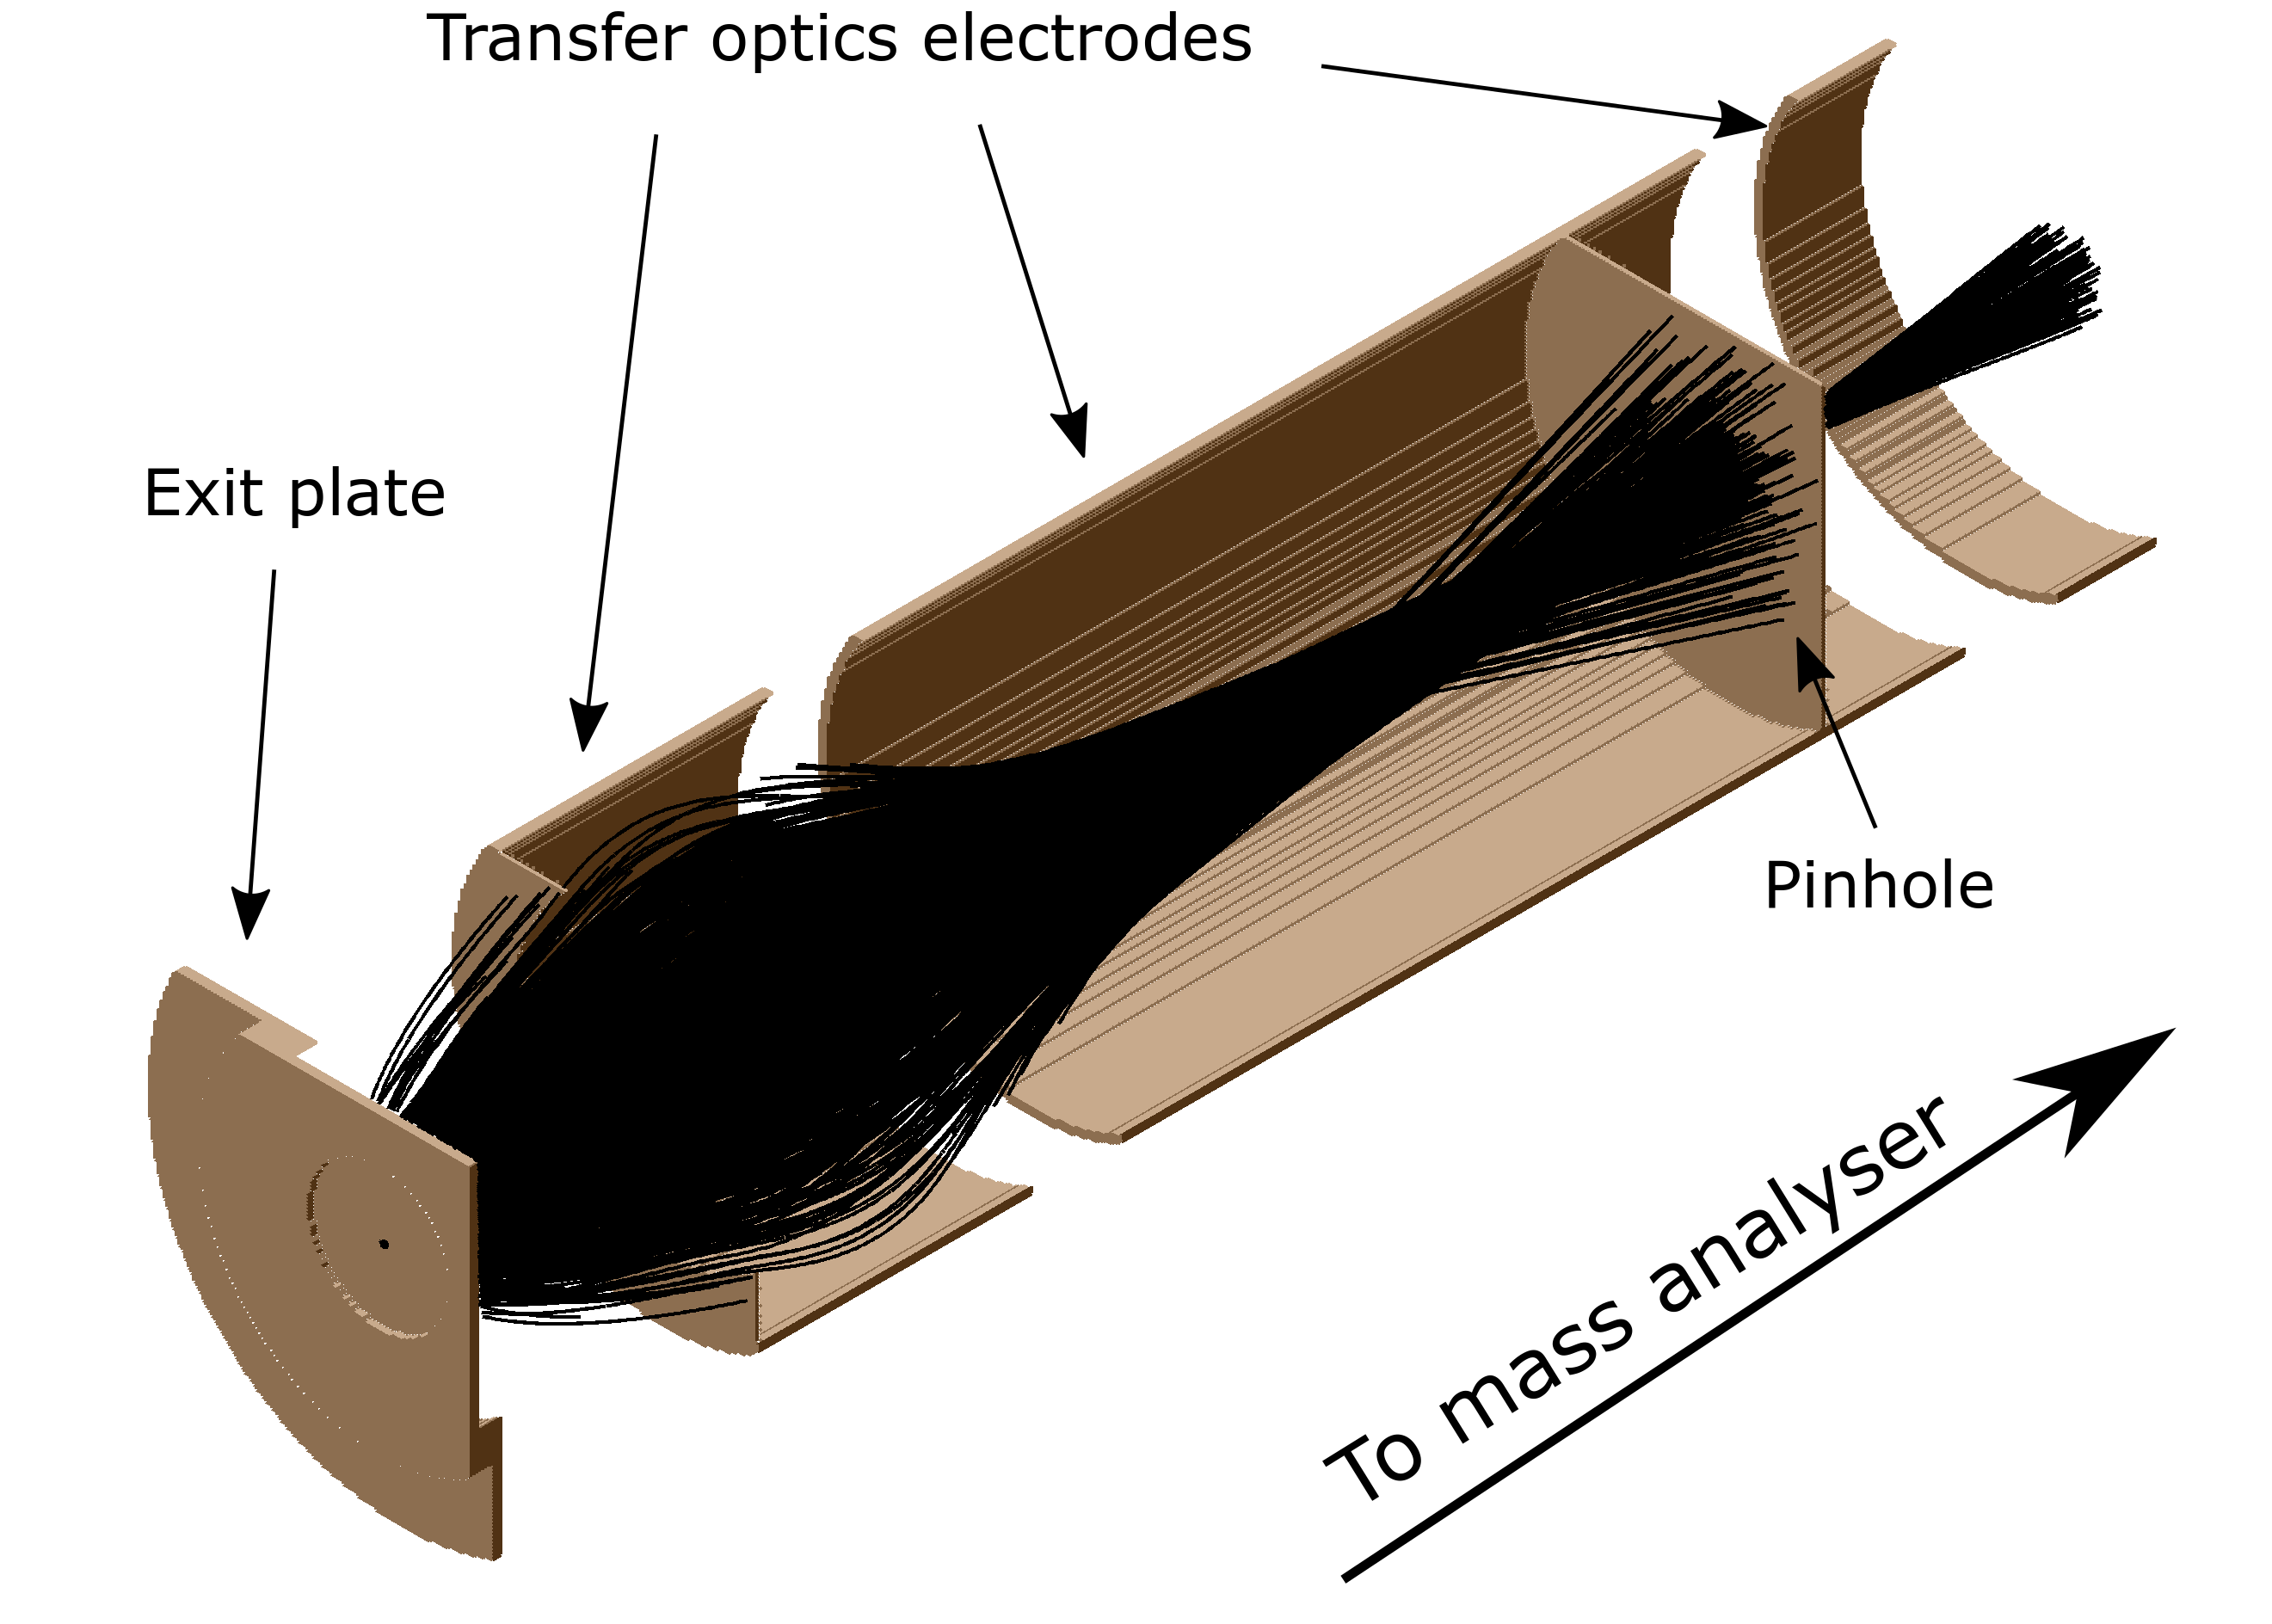
\includegraphics[width=0.6\linewidth]{pics/tf_names.png}
\centering
\caption[Simulation of the ion trajectories in the transfer lens region using SIMION\textsuperscript{\textregistered}.]{Simulation of the ion trajectories in the transfer lens region using SIMION\textsuperscript{\textregistered}. 1000 ions of \textit{m/z} 100 with kinetic energies uniformly distributed between 0 and 1 eV were flown.}
\label{fig:tl_simion}
\end{figure}


\subsection{Mass spectrometer}
The ion beam is transferred from the drift tube to the mass spectrometer (\acrshort{ms}) via the transfer optics. The MS detects the ions according to their mass-to-charge ratio and allocate them in a histogram-like plot mass spectrum.  The terms mass spectrometer and mass analyser will be used interchangeably.

The mass-to-charge ratio is abbreviated to \textit{\acrshort{mz}} and it refers to the ratio of the ions' mass divided by their charge. SI units are not used for the \textit{m/z}. For simplicity, atomic mass units (\acrshort{amu}) are used for the mass (1 amu = 1.66$\times$10$^{-27}$ kg) and the number of fundamental electric charges for the charge (1 e = 1.60$\times$10$^{-19}$ C). 
%Depending on the mass resolution of the MS, \textit{m/z}  is given as an integer (nominal mass) or as a real number (monoisotopic mass).

\subsubsection{Time-of-flight mass spectrometer}
The time-of-flight mass spectrometers  (\acrshort{tofms}, \autoref{fig:tof})  are  the most widely mass spectrometers used in PTR-MS. 
%
Their operating pressure is of 10$^{-7}$ mbar or less.

A ToF-MS works as follows: when ions reach the entrance of the MS (pulser region), a pulsed (tens of kHz) high voltage V of some kilovolts orthogonally repels them towards the other end of the flight tube. Lighter ions will gain more speed than heavier ions, which means that they will reach the detector faster. The time it takes an ion to reach the detector and its \textit{m/z} are related through \autoref{eq:tof2}, which comes from the energy balance in \autoref{eq:tof1}:
%
\begin{equation}
\label{eq:tof1}
qV =  \frac{1}{2} m\left(\frac{l}{t}\right)^2
\end{equation}
\begin{equation}
\label{eq:tof2}
t= \sqrt{\frac{m}{z} \frac{l^2}{2eV}}
\end{equation}
where \textit{m/z} is the mass-to-charge ratio of the ion, $l$ is the length of the flight tube, t is the flight time and $q = e z$ is the ion's charge.
This allows to calculate the \textit{m/z} of the ions as they are being collected at the detector and build the mass spectrum by measuring the ions' time of flight.



\begin{figure}%[ht]
\centering
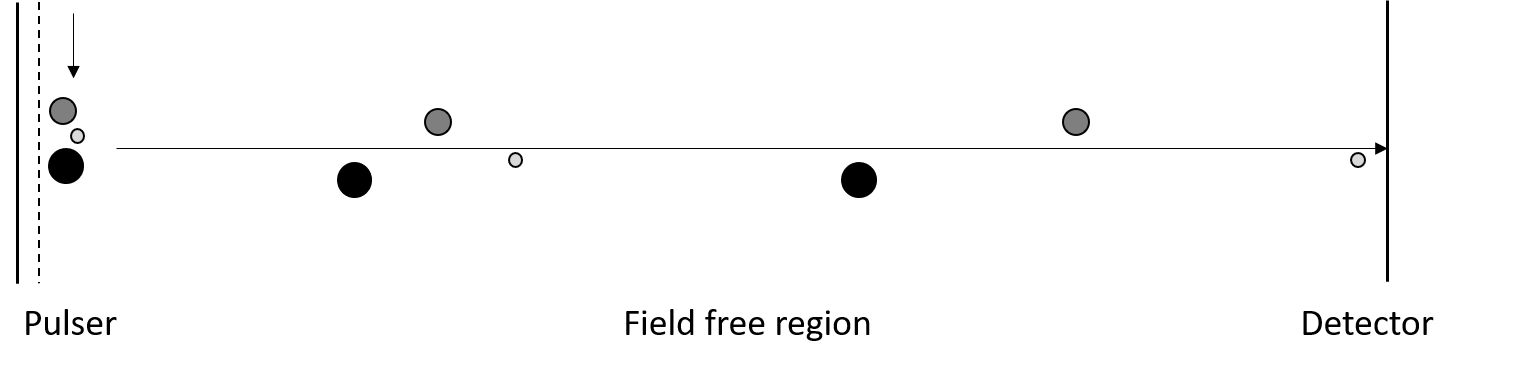
\includegraphics[width=0.8\linewidth]{pics/tofms.png}
\centering
\caption[Diagram of a linear time-of-flight mass spectrometer.]{Diagram of a linear time-of-flight mass spectrometer. Circles represent ions, being their diameter proportional to their mass-to-charge ratio.}
\label{fig:tof}
\end{figure}



\subsubsection{Reflectron}
A spatially spread distribution of ions of the same \textit{m/z} in the pulser region can result in different ion velocities, and hence being detected at different times, broadening the mass spectrum peaks.
%
To amend this a reflectron can be implemented in the flight tube of a ToF-MS.

A diagram showing how a reflectron works is provided in \autoref{fig:tofr}. It basically consists of a series of electrodes with increasing voltage that will reverse the trajectory of the ions. When a cloud of ions reaches the reflectron, ions of the same \textit{m/z} but going faster go deeper in it, having a longer flight distance than slower ions. This way, slow and fast ions of the same \textit{m/z} will reach the detector at the same time, having travelled different distances, yielding narrower peaks and  improved mass resolution. % when the mass spectrum is built.

\begin{figure}%[ht]
\centering
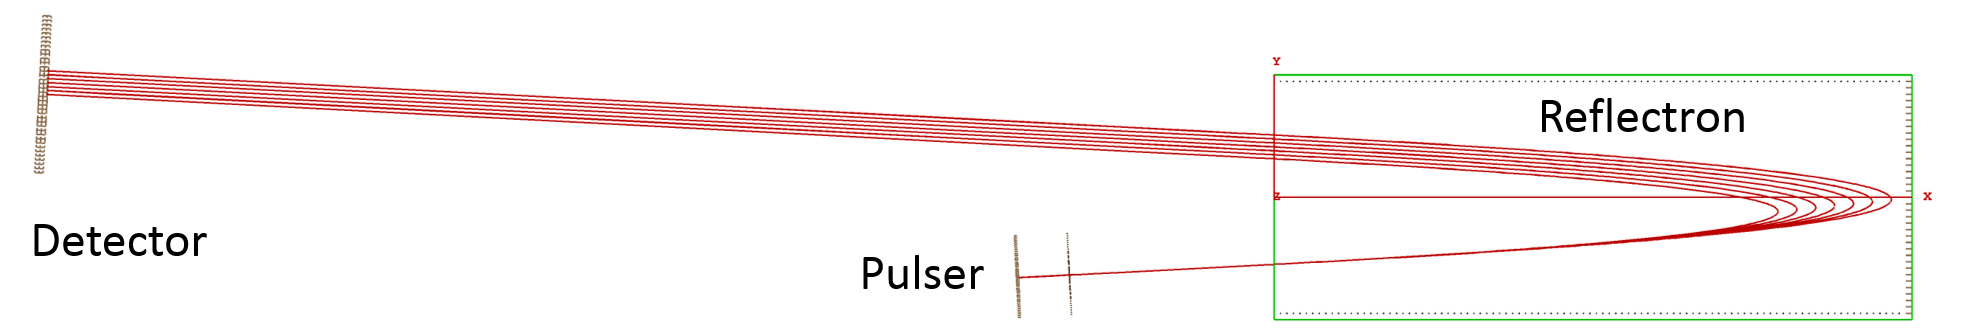
\includegraphics[width=0.8\linewidth]{pics/reflectron2.png}\label{fig:tofr_sim}
\caption{Schematic diagram of a flight tube with a reflectron showing the different trajectories of seven ions of the same \textit{m/z} with different initial velocities simulated  in SIMION\textsuperscript{\textregistered}.}
\label{fig:tofr}
\end{figure}




%\subsubsection{Time-of-flight vs quadrupole}
%Time-of-flight is the most commonly used but it is not the only type of mass spectrometers available for the the  in PTR-MS. Many instruments, typically older ones, use quadrupole instead of time-of-flight technology.


%A quadrupole consists of four parallel rods %(see \autoref{fig:quad})
%from which opposite rods will be at the same electric potential. Said potential is a combination of static and time-dependent fields for which only ions of a certain \textit{m/z} will have a stable trajectory. This allows to select the \textit{m/z} to be transmitted, and these ions will reach the detector at the end of the quadrupole.

%Compared to time-of-flight mass spectrometers, quadrupoles are more compact, robust and cheap. On the other hand, quadrupoles also have some disadvantages. By their principle of operation, quadrupoles need to do a mass scan to build up the mass spectrum. This makes them much slower than time-of-flight devices, which can take measurements in up to 200 ms and are therefore suitable for transient experiments like desorptions. Similarly, the mass resolution of quadrupoles doesn't allow to distinguish between isobaric compounds, which can be done using a time-of-flight mass filter. Also, there is an upper limit for quadrupoles' mass range, which in theory is not a problem in time-of-flight devices although a mass limitation can arise from the use of reflectrons.

%\begin{figure}%[ht]
%\centering
%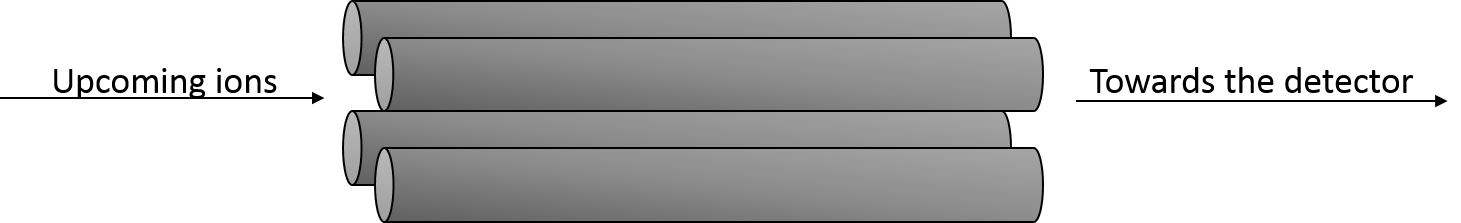
\includegraphics[width=0.8\linewidth]{pics/quad.png}
%\centering
%\caption{Schematic diagram of a quadrupole mass filter.}
%\label{fig:quad}
%\end{figure}

\subsubsection{Detector}
Prior to detection, the individual ion signal needs to be amplified to a detectable level. A common pre-amplification setup consists of two microchannel plates (MCPs), which are circular plates of a few millimetre of thickness with an array of tubes that go from one face to the other. These tubes form an angle with the ion trajectory and the second MCP is rotated 180$^{\circ}$ from the first one as shown in \autoref{fig:det} so ions cannot go through without hitting the plates.

Incoming ions are accelerated to $\sim$2 kV before they hit the MCPs' walls. Said MCPs are made of a high resistive material with a secondary electron emission factor greater than one, so that when the incoming ion hits it,  one or more electrons are emitted per collision, generating an avalanche that can amplify a single event by up to a factor of 10$^8$. The cascade electron signal will then reach the anode, where the time-to-digital converter (TDC) will process the analogue signal and convert it into digital.


\begin{figure}%[ht]
\centering
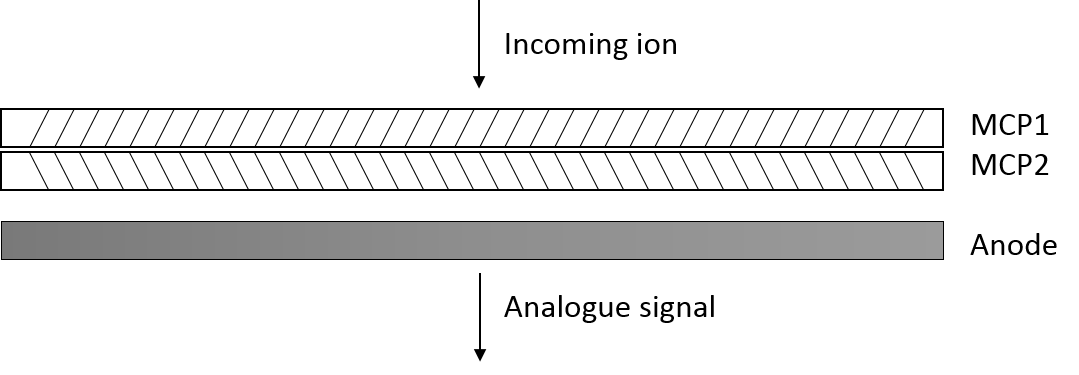
\includegraphics[width=0.6\linewidth]{pics/mcp.png}
\centering
\caption{Schematic diagram of a MCP detector.}
\label{fig:det}
\end{figure}


\subsubsection{Calibration}
As any other scientific instrument, the PTR-ToF-MS must be calibrated before performing any experiment. Note that  this section  refers to calibration as the method to calculate the mass conversions parameters, not the calibration to calculate a concentration from an ion signal. The mass conversions parameters can be calculated by selecting some reference peaks and assigning them their exact \textit{m/z}.
Some peaks that can be used to calibrate the instruments are the $^{18}$O isotope of hydronium (H$_3^{18}$O$^+$, \textit{m/z} 21.023), NO$^{+}$ (m/z 29.998) and  NO$_2^{+}$ (m/z 45.993). 
%
It is also useful to include peaks from the larger end of the mass spectrum (i.e. \textit{m/z} >200). If a single analyte is being studied (i.e. not a mixture), its protonated parent ion can be used.
%It is also useful to use the analyte ion that will be measured as a calibration peak and other peaks resulting from compounds present in air, like protonated acetone ((C$_3$H$_6$O)H$^+$, \textit{m/z} 59.050).
%
The TDC uses \autoref{eq:cal} for this task doing a least squares fitting:
%
\begin{equation}
\label{eq:cal}
m\slash z =  \left(\frac{t-t_0}{C_b}\right)^2
\end{equation}
where \textit{m/z} is the mass-to-charge ratio, t is the ion's time-of-flight, and t$_0$ and C$_b$ are parameters that depend in the mass range the instrument will measure and in some experimental quantities like the length of the flight tube. Note that this equation is the same as \autoref{eq:tof2} for t$_0$ = 0 and $C_b$ = $l/\sqrt[]{2eV}$.



\section{Data post-processing and computational methods}
%In this section I explain how the post-processing of the data is done.







\subsection{Data acquisition, visualisation and treatment}

The analogue data acquired by the PTR-ToF-MS is translated into digital files by \acrshort{tdc} to be visualised and analysed  with the proper software. An experiment can consist in either a static measurement, yielding a stable signal throughout the experiment, or a transient measurement, where the ion signals are time-dependent. These different types of experiments are usually acquired as a mass spectrum  in the form of a Galactic .spc  file from Thermo Fisher Scientific\textsuperscript{\textregistered}, or as a temporal evolution of the mass spectrum, in the form of a binary .lst file, respectively.

As mentioned earlier, a mass spectrum is the histogram-like plot of the counts of detected ions as a function of their \textit{m/z} which, in our case, is stored in .spc files.
\autoref{fig:grams}(a) shows an example of a mass spectrum visualised with the Thermo Fisher Scientific\textsuperscript{\textregistered}  GRAMS/AI\textsuperscript{TM}  Spectroscopy Software, which is adapted by KORE Technology Ltd to be used with their equipment.
The software does the time to \textit{m/z} conversion following \autoref{eq:cal}.


Transient experiments are stored in %raw files called
.lst files.
 These %are binary
 files  record the timestamp in microseconds of each event in three consecutive bytes in hexadecimal notation, with the most significant byte first, and they are accompanied by a text  (.ini) file containing information about the experiment.
An event can be either the start of a cycle in the detector, always indicated by 0x000000 (i.e. t = 0 µs), or a detected ion (for instance, an ion detected at t = 12500 µs would be recorded as 0x0030D4).
 Therefore an .lst file holds all the information about the experiment and can be plotted as either a cumulative mass spectrum as a function of the \textit{m/z} or as a transient of selected ion signals as a function of the experiment time.
The software GRAMS/AI\textsuperscript{TM} allows to open the .lst files as a mass spectrum, like that in \autoref{fig:grams}(a), or as the time-evolution of some particular \textit{m/z}, as shown in \autoref{fig:grams}(b). For the latter plot, the so-called regions of interest must be selected before starting the experiment 
to display targeted ion signals. 
%, by selecting the left and right ends of intervals of interest whose ion count will be integrated, displayed and updated as the data is acquired.
%This is  useful in conjunction with the TDU, as it will be explained in the .................... %results section.

%advantage: real time monitoring as the data is recorded



\begin{figure}%[t]
\centering
\sidesubfloat[]{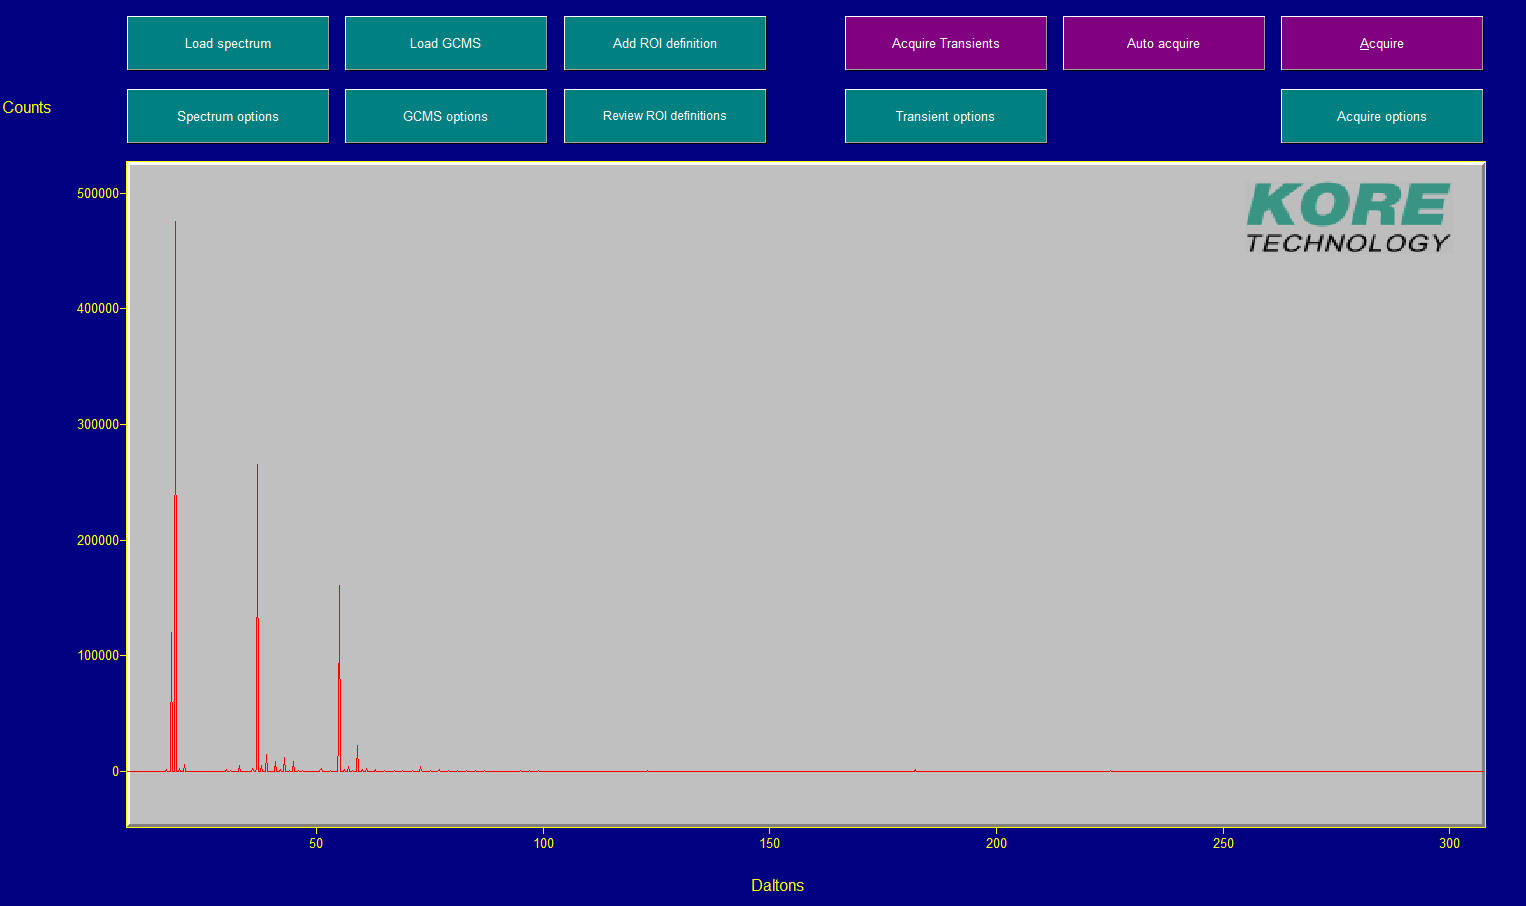
\includegraphics[width=0.9\linewidth]{pics/background_120Td.png}}

\sidesubfloat[]{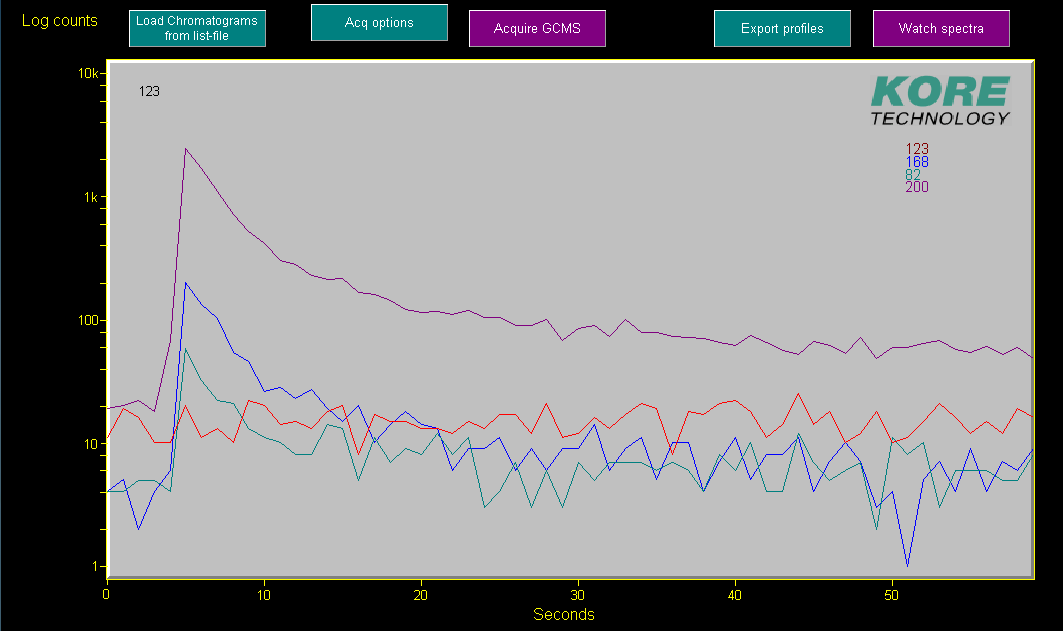
\includegraphics[width=0.9\linewidth]{pics/MeEcg_des2.png}}
\caption{Screenshot of the GRAMS/AI\textsuperscript{TM} user interface for the PTR-ToF-MS instrument manufactured by KORE Technology Ltd showing (a) an example of mass spectrum, and (b) an example of transient experiment data.}
\label{fig:grams}
\end{figure}



Additionally, the Matlab\textsuperscript{\textregistered} command \textit{tgspcread()} is compatible with  Galactic .spc files from Thermo Fisher Scientific\textsuperscript{\textregistered}.
%
This command imports all the fields in the data file into an object-oriented data type called \textit{struct}, which allows quick and easy extraction and manipulation of large amounts of data.
 In the case of the .lst files, the extraction of the data has to be done without help from any library. It is a bit more tedious, as it requires reading the hexadecimal file, building the mass spectra using the parameters stored in the .ini file, do the time-mass conversion and  extract the \textit{m/z} of interest for transient experiments.
 


% With a PTR-MS instrument, a lot of data can be acquired quite quickly so basic programming knowledge comes in handy when dealing with these big data sets.
% One of the best options is to use the Matlab\textsuperscript{\textregistered} command \textit{tgspcread()}, which reads  Galactic .spc files from Thermo Fisher Scientific\textsuperscript{\textregistered}. This imports all the fields in the data file into an object-oriented data type called \textit{struct}, which allows quick and easy extraction and manipulation of large amounts of data.
% In the case of the .lst files, the extraction of the data has to be done without help from any library. It is a bit more tedious, as it requires reading the hexadecimal file, building the mass spectra using the parameters stored in the .ini file, do the time-mass conversion and  extract the \textit{m/z} of interest for transient experiments.
% Using this  as starting point, I wrote my own code to do the data analysis. It extracts all the data from a whole study or experiment to analyse it in Matlab\textsuperscript{\textregistered}, measuring peak positions using the FWHM of the peaks, calculating peak intensities, extracting transient data, subtracting background signals and assigning possible chemical compositions.




\subsection{Calculation of ion intensities}
Once the data is acquired and stored in the files explained in the previous section, it can be analysed and plotted for interpretation, although there are some concerns to %deal with
take into account when doing this.

The counting electronics in the PTR-ToF-MS assumes that each pulse measured at the MCP corresponds to one ion. This can be not true if two or more ions arrive at the detector very close together and their analogue signals overlap so that the TDC translates it as a single event. This phenomenon is known as saturation and happens more often when a high concentration of a compound is being measured.
At a given \textit{m/z}, the maximum number of counts per second the instrument can measure corresponds to the number of cycles per second of the mass spectrometer, which is the number of times the ions are pulsed each second. In other words, at a certain \textit{m/z} only one ion per cycle can be measured. Therefore, a compromise must be found when the experiment is being designed to avoid situations of saturation while getting a suitable signal.
This is given by the rule of thumb that says that saturation occurs when the ion signal at a certain \textit{m/z} is more than 60\% of the cycles per second in the time of flight.
This means that a peak can present saturation effects even before showing a distorted shape. For instance, for a cycle length of 36 µs, the mass spectrometer will be pulsing at a rate of $\sim$27777 cycles per second.
In this case, the 60\% saturation limit would be at an ion signal of $\sim$16666 cps.

%Dead time...........

Peak saturation situations should be avoided when it occurs at product ion peaks, as it can carry other effects like reagent ion depletion.
However, saturation is commonly observed for the reagent ion peaks, whose intensities can be calculated using the suitable isotopes in each case.
%in some scenarios they can be worked around by calculating the ion intensities using the suitable isotopes in each case.
The $^{18}$O isotope peak is used to calculate the reagent ion intensities of  H$_3$O$^+$ or O$_2^+$ as their more abundant $^{16}$O peak is often saturated.
The natural composition of oxygen is $^{16}$O (99.76\%), $^{17}$O (0.03\%) and $^{18}$O (0.21\%) \cite{nistoxygen}.
%This applies to the three most used reagent ions in \acrshort{scims}.
The $^{18}$O isotope is found at \textit{m/z} 21.023 for H$_3$O$^+$ and at m/z 33.994 for O$_2^+$.
However, for NO$^+$ it is better to use the $^{15}$NO$^+$ at \textit{m/z} 30.995 rather than the N$^{16}$O$^+$ at \textit{m/z}  32.002 for two reasons: the $^{15}$NO$^+$  isotope  is more abundant  and also it does not interfere with the  signal of the isobaric compound O$_2^+$  at \textit{m/z}  32.

The $^{13}$C isotope is often used to calculate product ion intensities in saturated peaks and to verify composition assignments if the mass resolution is not enough to distinguish between isobaric compounds.
It is the second most abundant isotope (1.07\%) after  $^{12}$C (98.93\%), with  $^{14}$C is only present at 1 ppt \cite{nistcarbon}.
$^{13}$C is obviously more useful with bigger molecules because normally the bigger the molecule, the more carbons it will have, yielding a peak intensity of more than 10\% at %\textit{(m+1)/z} 
\textit{m/z} + 1 of that at \textit{m/z} for molecules with ten or more carbon atoms.
Of special interest are as well the halogenated compounds containing Cl or Br, which show  very characteristic isotopic  peaks. $^{35}$Cl and $^{37}$Cl are naturally present at abundances of 75.76\% and 24.24\%, while for $^{79}$Br and $^{81}$Br these are 50.69\% and 49.31\%, respectively \cite{nistcl,nistbr}.
Thus,  molecules containing a single Cl atom show a pattern of peaks whose intensity is ca. 3:1 at  \textit{m/z} and %\textit{(m+2)/z}
\textit{m/z} + 2, while for molecules with two Cl atoms this is 9:6:1 at  \textit{m/z}, %\textit{(m+2)/z}
\textit{m/z} + 2 and %\textit{(m+4)/z}
\textit{m/z} + 4. 
For  molecules with a single Br this is approximately 1:1 at  \textit{m/z} and %\textit{(m+2)/z}
\textit{m/z} + 2 while for two Br atoms it is 1:2:1 at \textit{m/z}, %\textit{(m+2)/z}
\textit{m/z} + 2 and %\textit{(m+4)/z}
\textit{m/z} + 4.

With these considerations in mind, for the rest of this thesis when an ion's \textit{m/z} is given with a chemical composition, it will refer to the most abundant isotopologue.
%It is also quite common to show the ion signal in normalised counts per second (\acrshort{ncps}) by normalising the ion signals to 10$^6$ counts of reagent ion signal. For this, the proton affinity of the analyte must be known because proton transfer from the water clusters can also occur and their ion signal must be considered when calculating the ncps. However, in most of this thesis  the data is shown in raw cps to ease the comparison with other instruments, after being usually repeated two times and subtracted the background signal.
In  this thesis  the data is either given in branching percentages (also referred to as branching ratios, BR, or product ion distributions, PID) 
or in raw counts per second, %cps to ease the comparison with other instruments,
after being  replicated two or three times, averaged and background subtracted.










%depletion

%Another effect to take into account is reagent ion depletion.
%This occurs when the concentration of the analyte is too high
%If the reagent ion signal is depleted, the sensitivity of the instrument is compromised, as there are not enough ions available to protonate (or, in general, to ionise) the analyte.
%It can occur at the same time as saturation for the product ions of the analyte but not necessarily.
%The only solution for this depletion is repeating the experiment with a lower concentration or higher  dilution.





%As stated before, proton donation to the targeted analyte comes from the collisions with the reagent ions, so it is crucial to monitor their signal to know the amount of available protons to be transferred to the analyte.

%The signal of the hydronium and its clusters as a function of the drift tube voltage in both DC mode and RF mode is shown in %\autoref{fig:ri}.
%These agree with the reagent ion signals previously observed \cite{price1977new}.


%The reagent ions' dependence with the voltage in DC mode is very different to that in RF mode. In DC mode the clusters break apart as the drift voltage increases. On the other hand, the RF field in RF mode delivers an extra collisional energy that breaks the clusters apart independently of the drift voltage. Also, this RF field can create potential wells for the lighter masses generating a low-mass cut-off of the transmission \cite{Chung123}.

%The measured reagent ion signal depends on the clustering/declustering reactions and the transmission of the instrument. Furthermore, clustering depends on humidity, collisional energy (E/N) and drift time. The higher the pressure in the cathode, the more hydronium is produced but it also will tend to create hydrogen bonds with other ions. Moreover, the higher the collisional energy, the more collisions the clusters will undergo, making them dissociate eventually. And last, the longer the drift time (at a given collisional energy), the more time the ions have to break apart through collisions.


% this is shown in the RF chapter
%\begin{figure}%[h]
%\centering
%\sidesubfloat[]{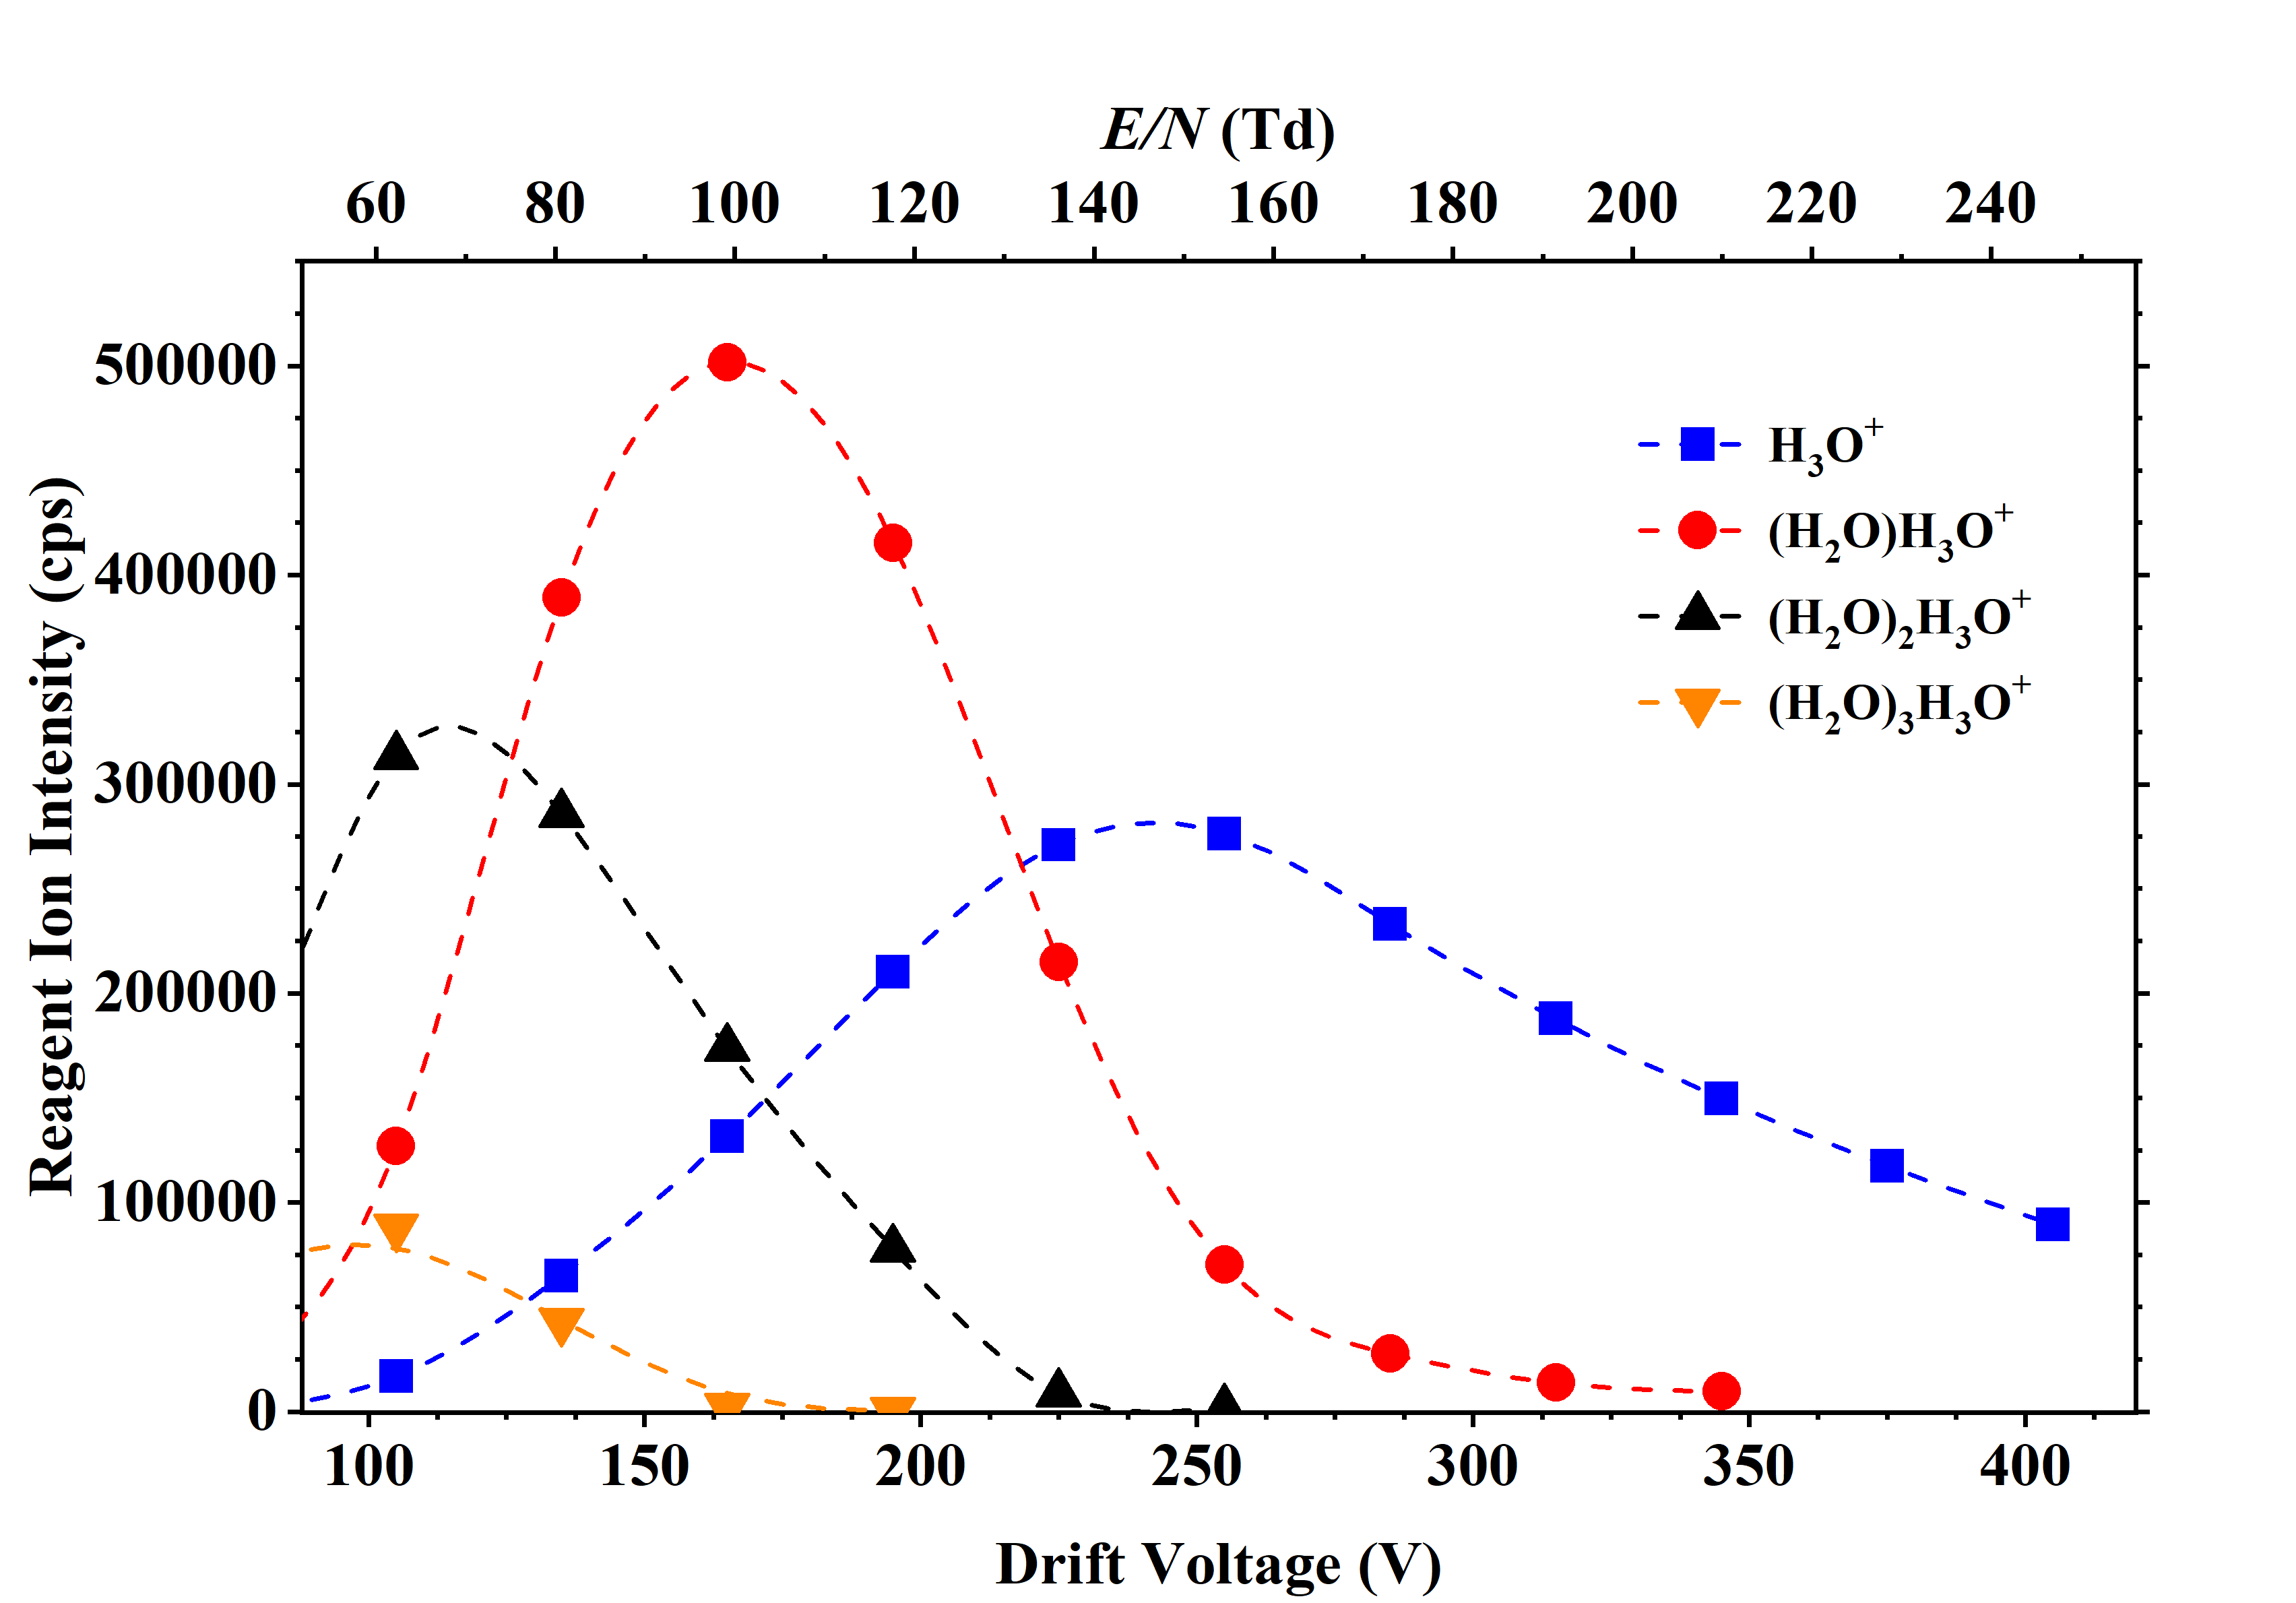
\includegraphics[width=0.6\linewidth]{pics/RInitros.png}\label{fig:ri1}}

%\sidesubfloat[]{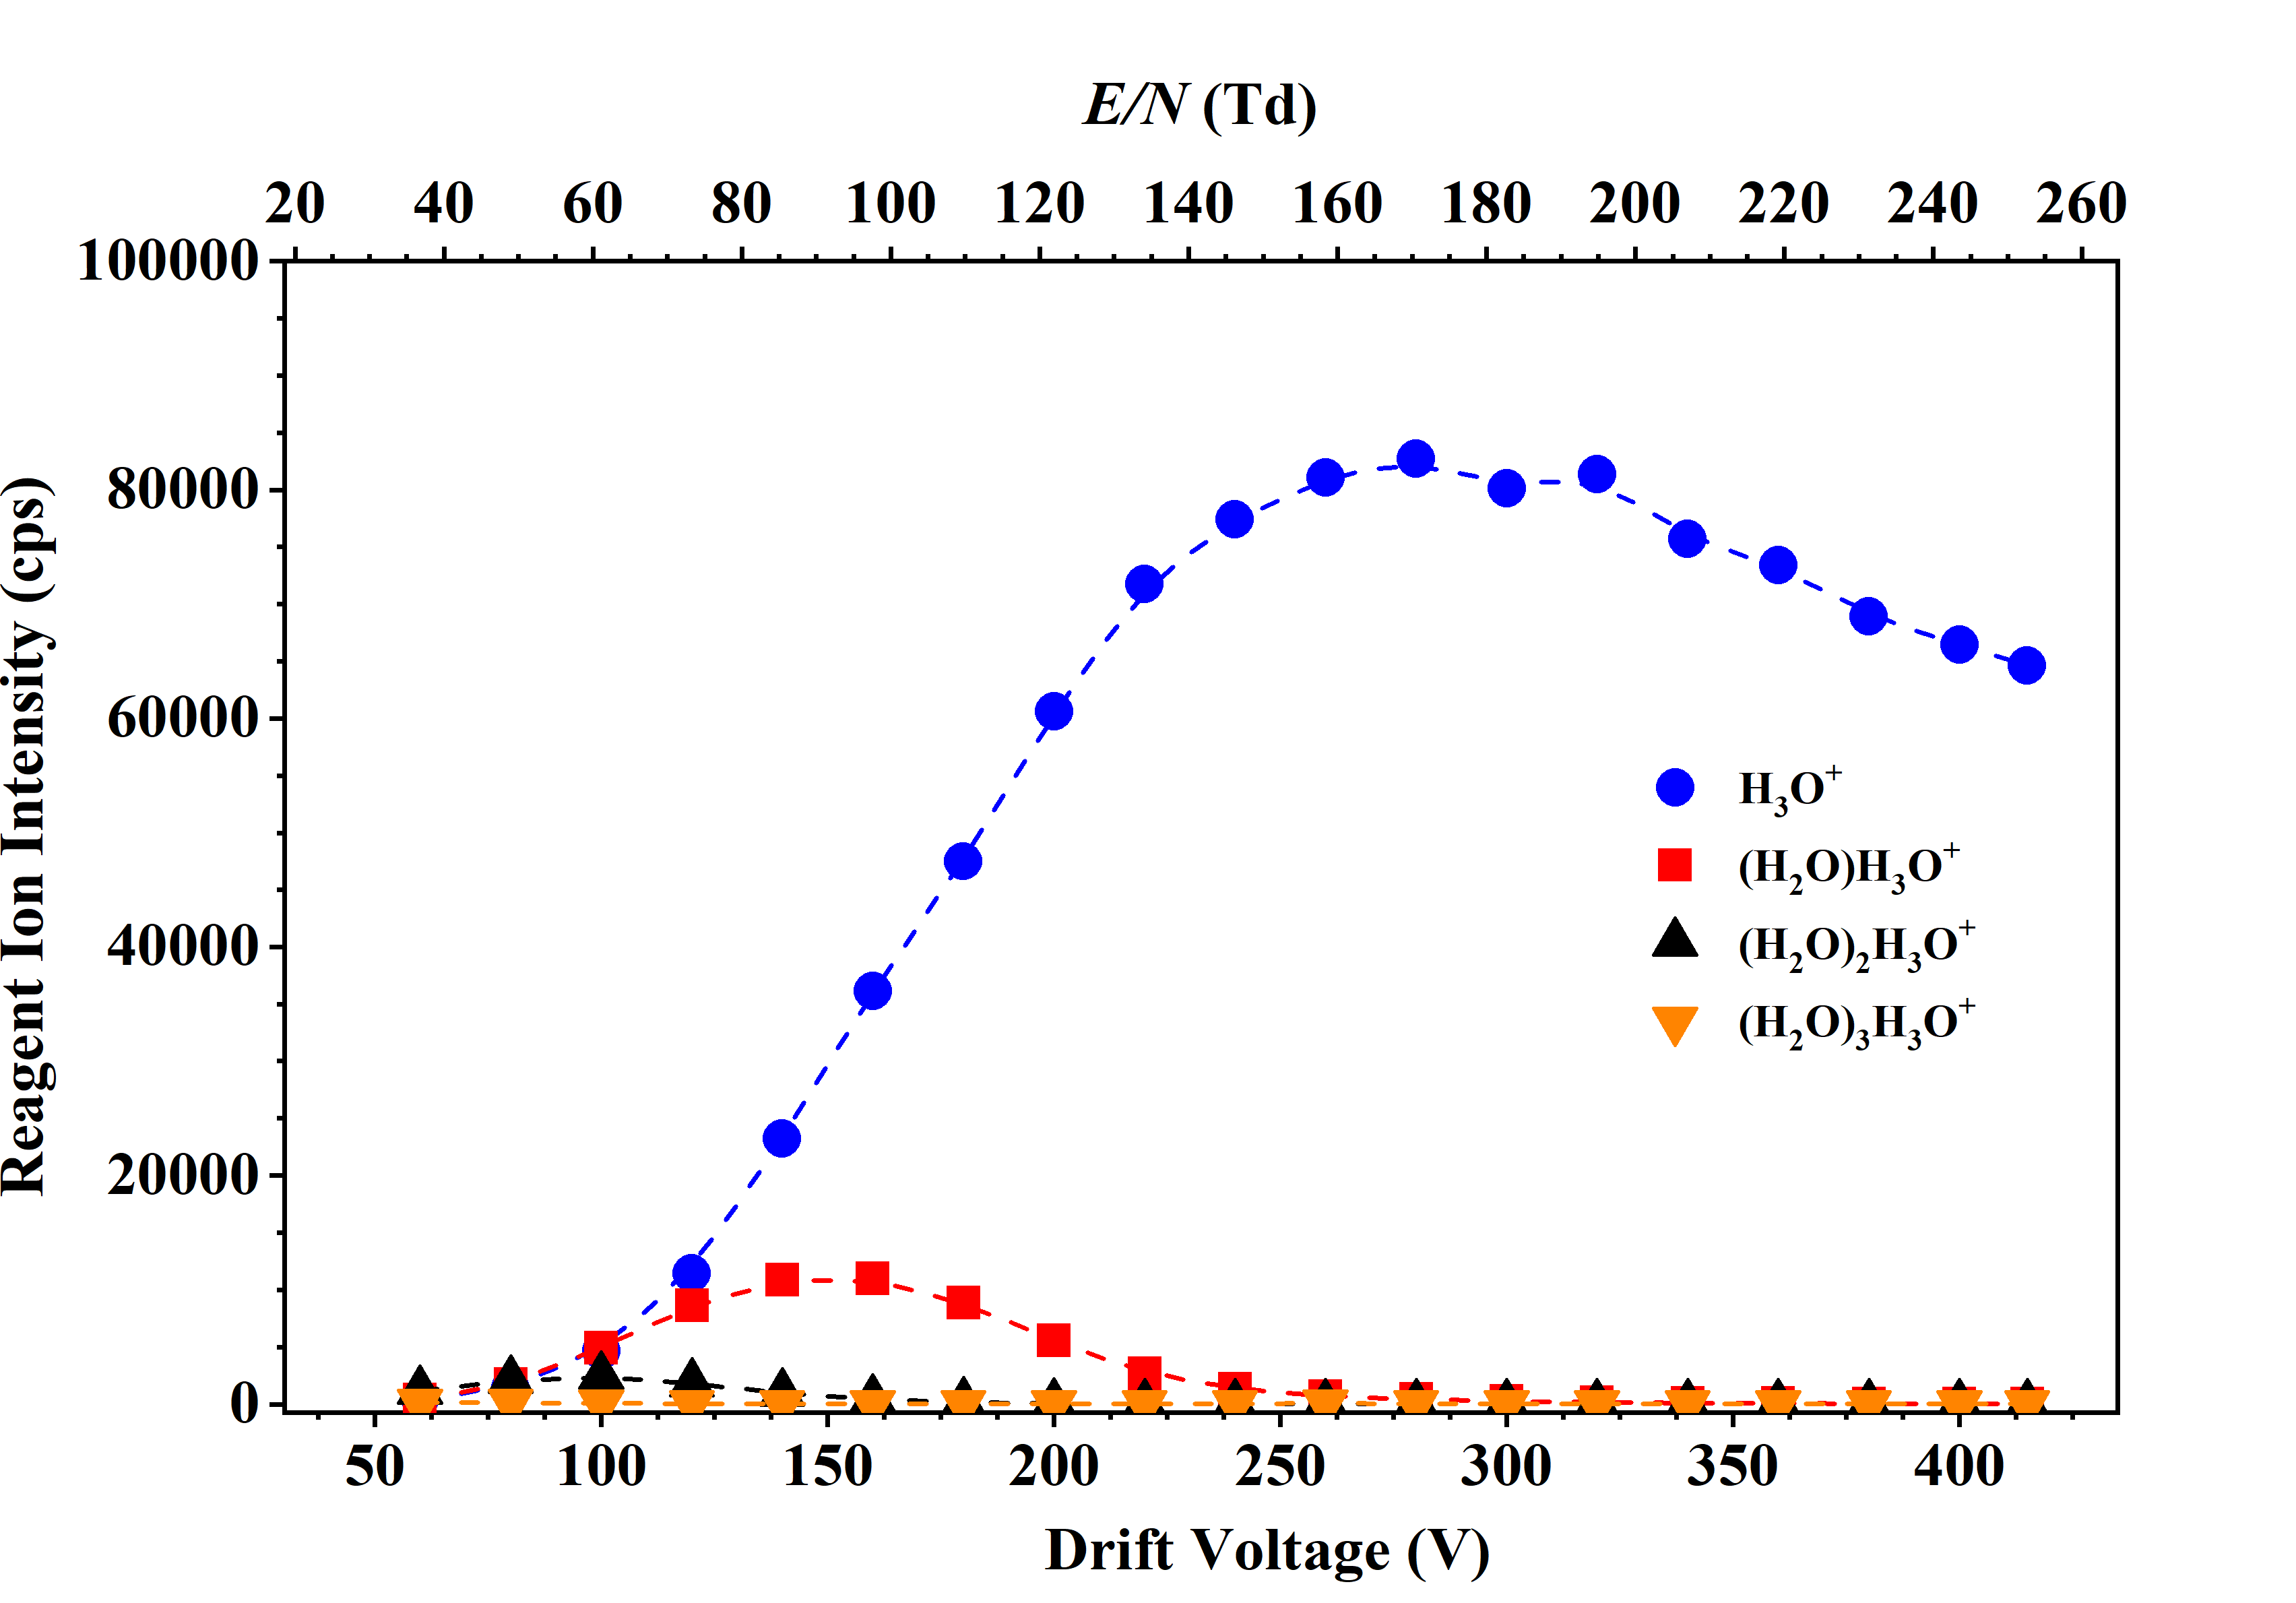
\includegraphics[width=0.6\linewidth]{pics/coc-RI.png}}

%\sidesubfloat[]{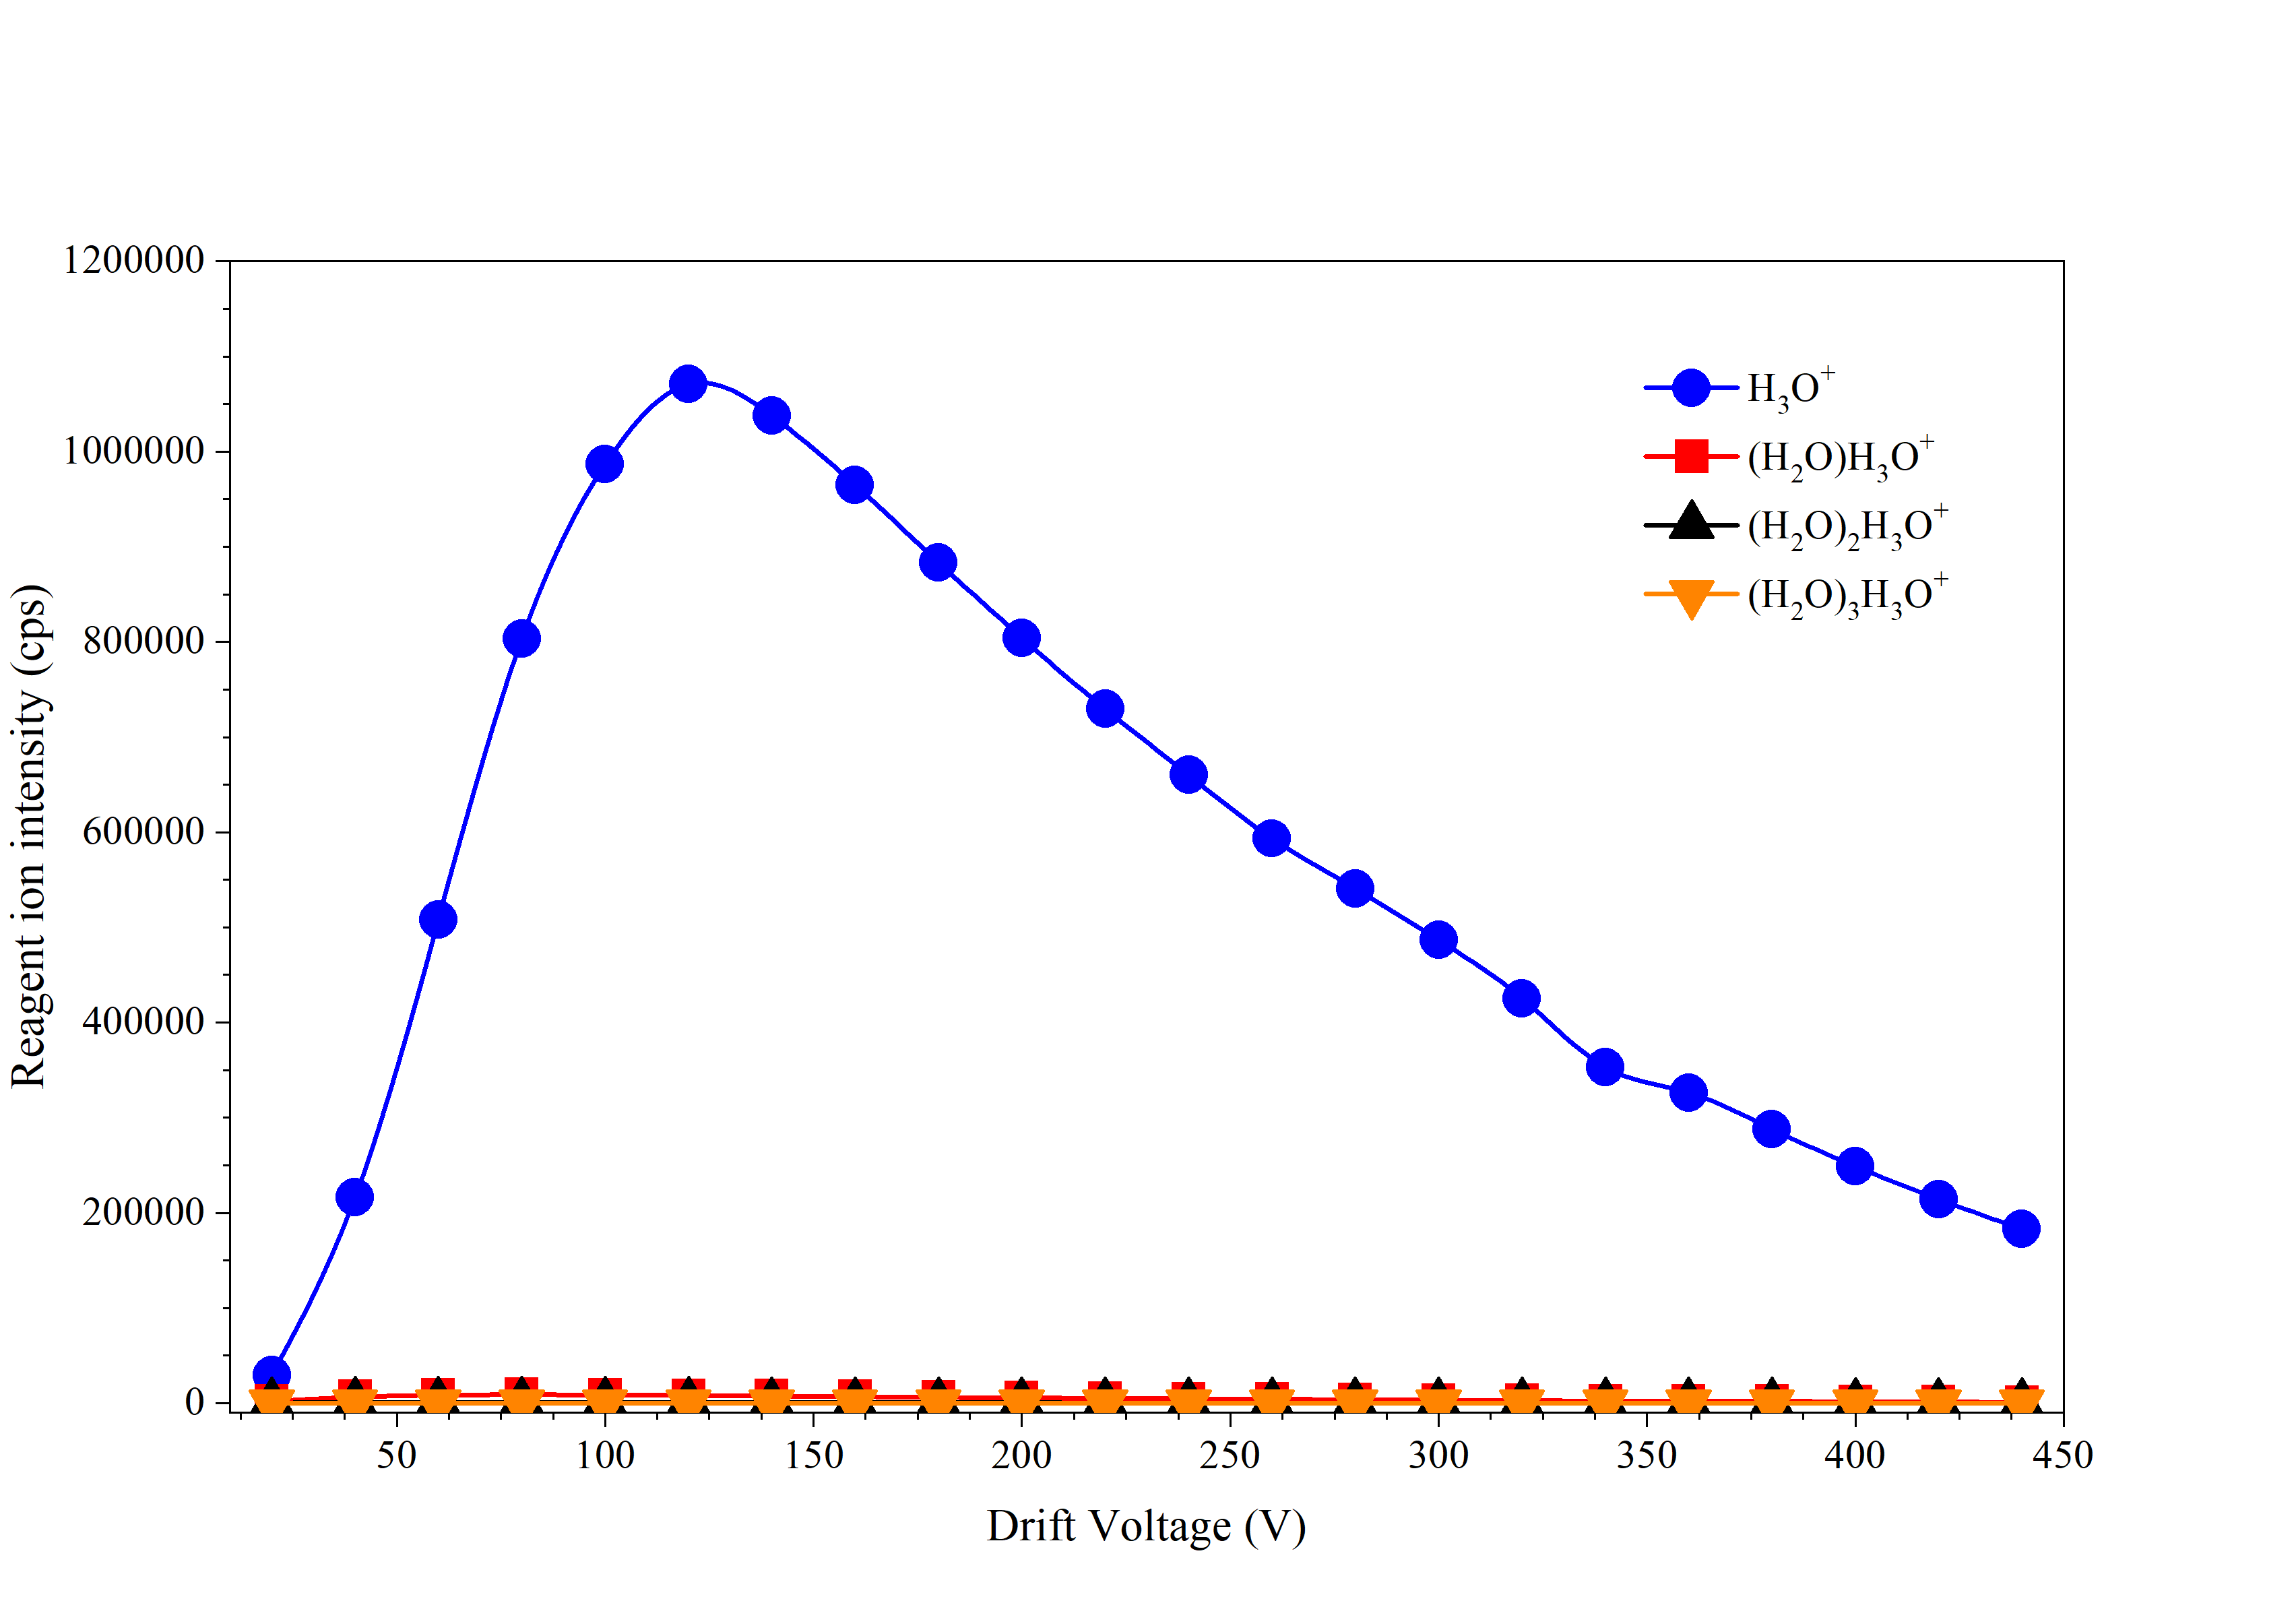
\includegraphics[width=0.6\linewidth]{pics/DPM_clusters_dry_RF.png}%water_RF.png}\label{fig:ri2}}
%\caption{Ion signal in counts per second (cps) for the reagent ions in (a) DC mode and (b) RF mode at 100$^{\circ}$C and 1 mbar. \textbf{Bottom one is from Lynx (MkII reactor)}}
%\label{fig:ri}
%\end{figure}













\subsection{Fast switching software}\label{sec:fs_data}
Analysing data from fast switching experiments can be tedious if needed to be done  manually file by file.
%
For this purpose, %and knowing already how to work with the experiment files, 
it was useful to write a script in Matlab\textsuperscript{\textregistered}  including  a graphical user interface to analyse the data in a quicker way.
%
This interface is shown in \autoref{fig:fss}.
It basically imports the suitable files, opens the cumulative mass spectrum to select the regions of interest, calculates and plots the ion intensities splitting the data in frames (i.e. each of the time intervals in which the drift tube is kept at the same \textit{E/N}), and exports the data to an excel file in both counts per second and branching ratios together with the experiment time and the \textit{E/N}.
%
Note that different colours are used in the raw and averaged data to ease the visualisation.

\begin{figure}%[t]
\centering
\sidesubfloat[]{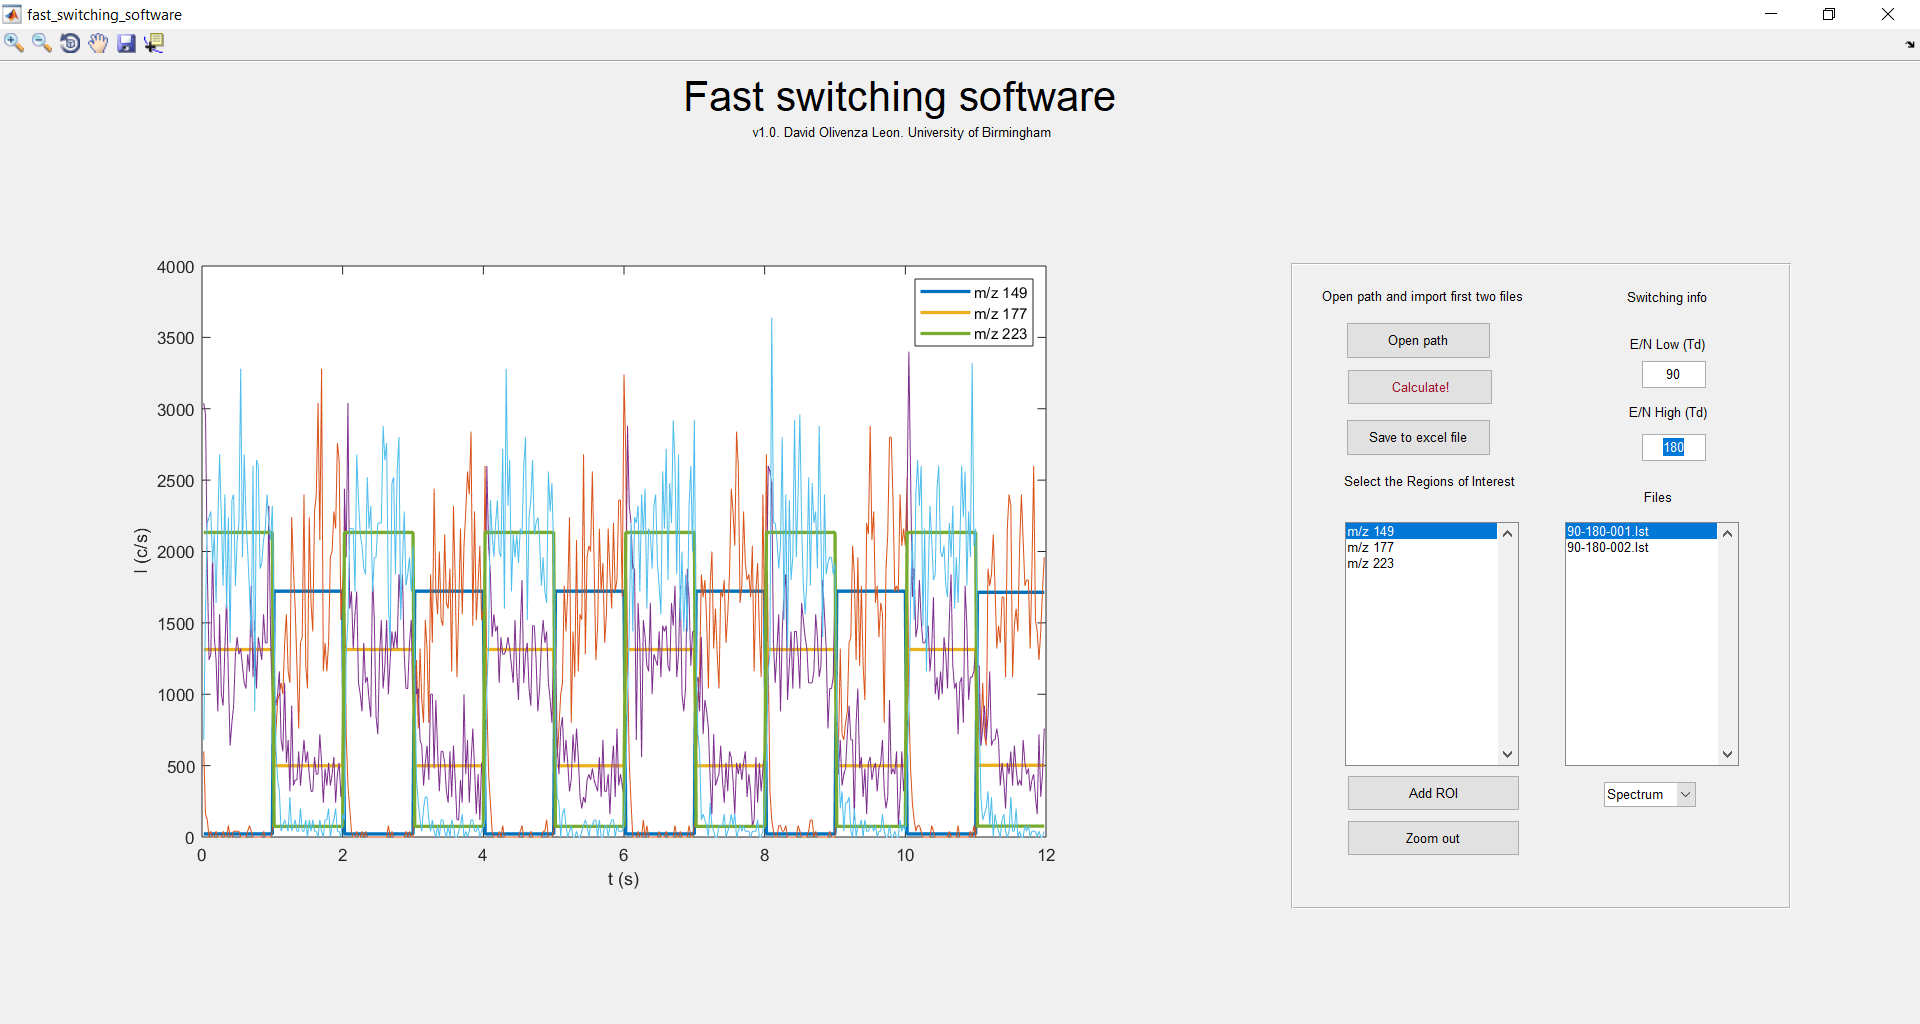
\includegraphics[width=0.9\linewidth]{pics/fss.png}}

\sidesubfloat[]{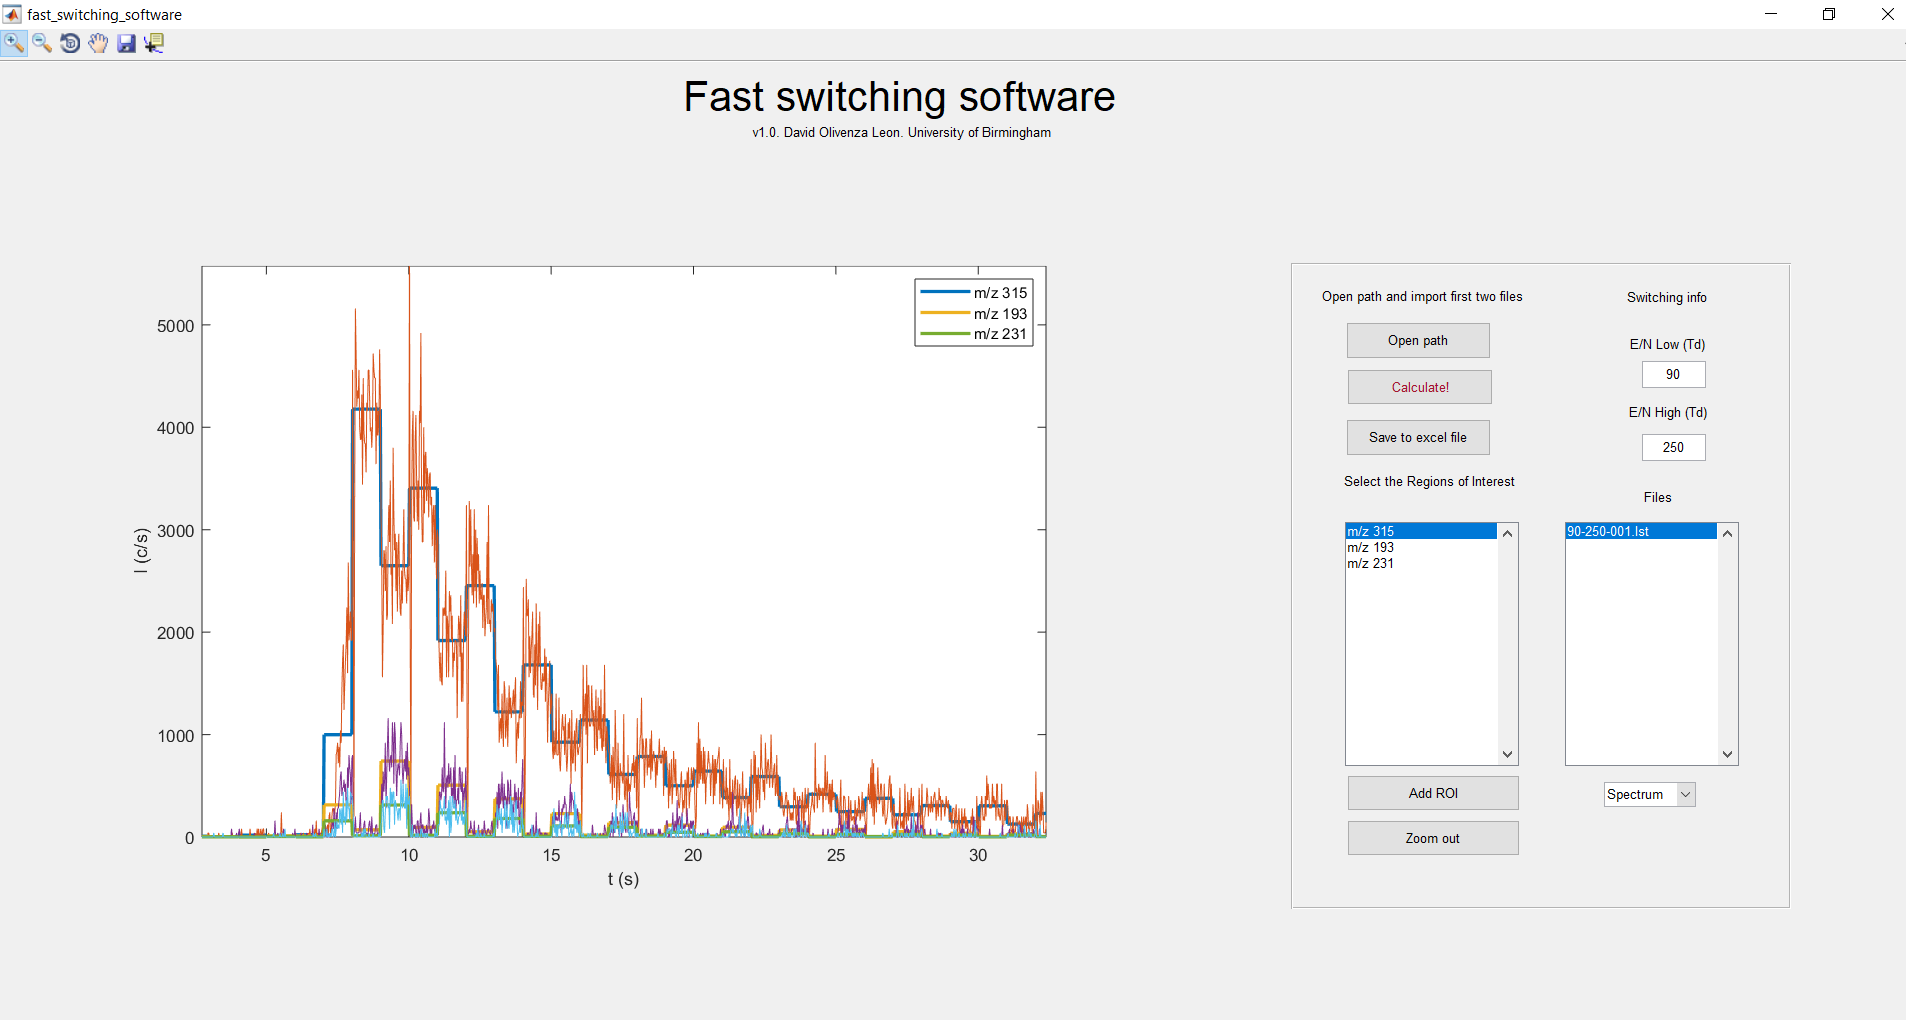
\includegraphics[width=0.9\linewidth]{pics/fs_CBD.png}}
%\sidesubfloat[]{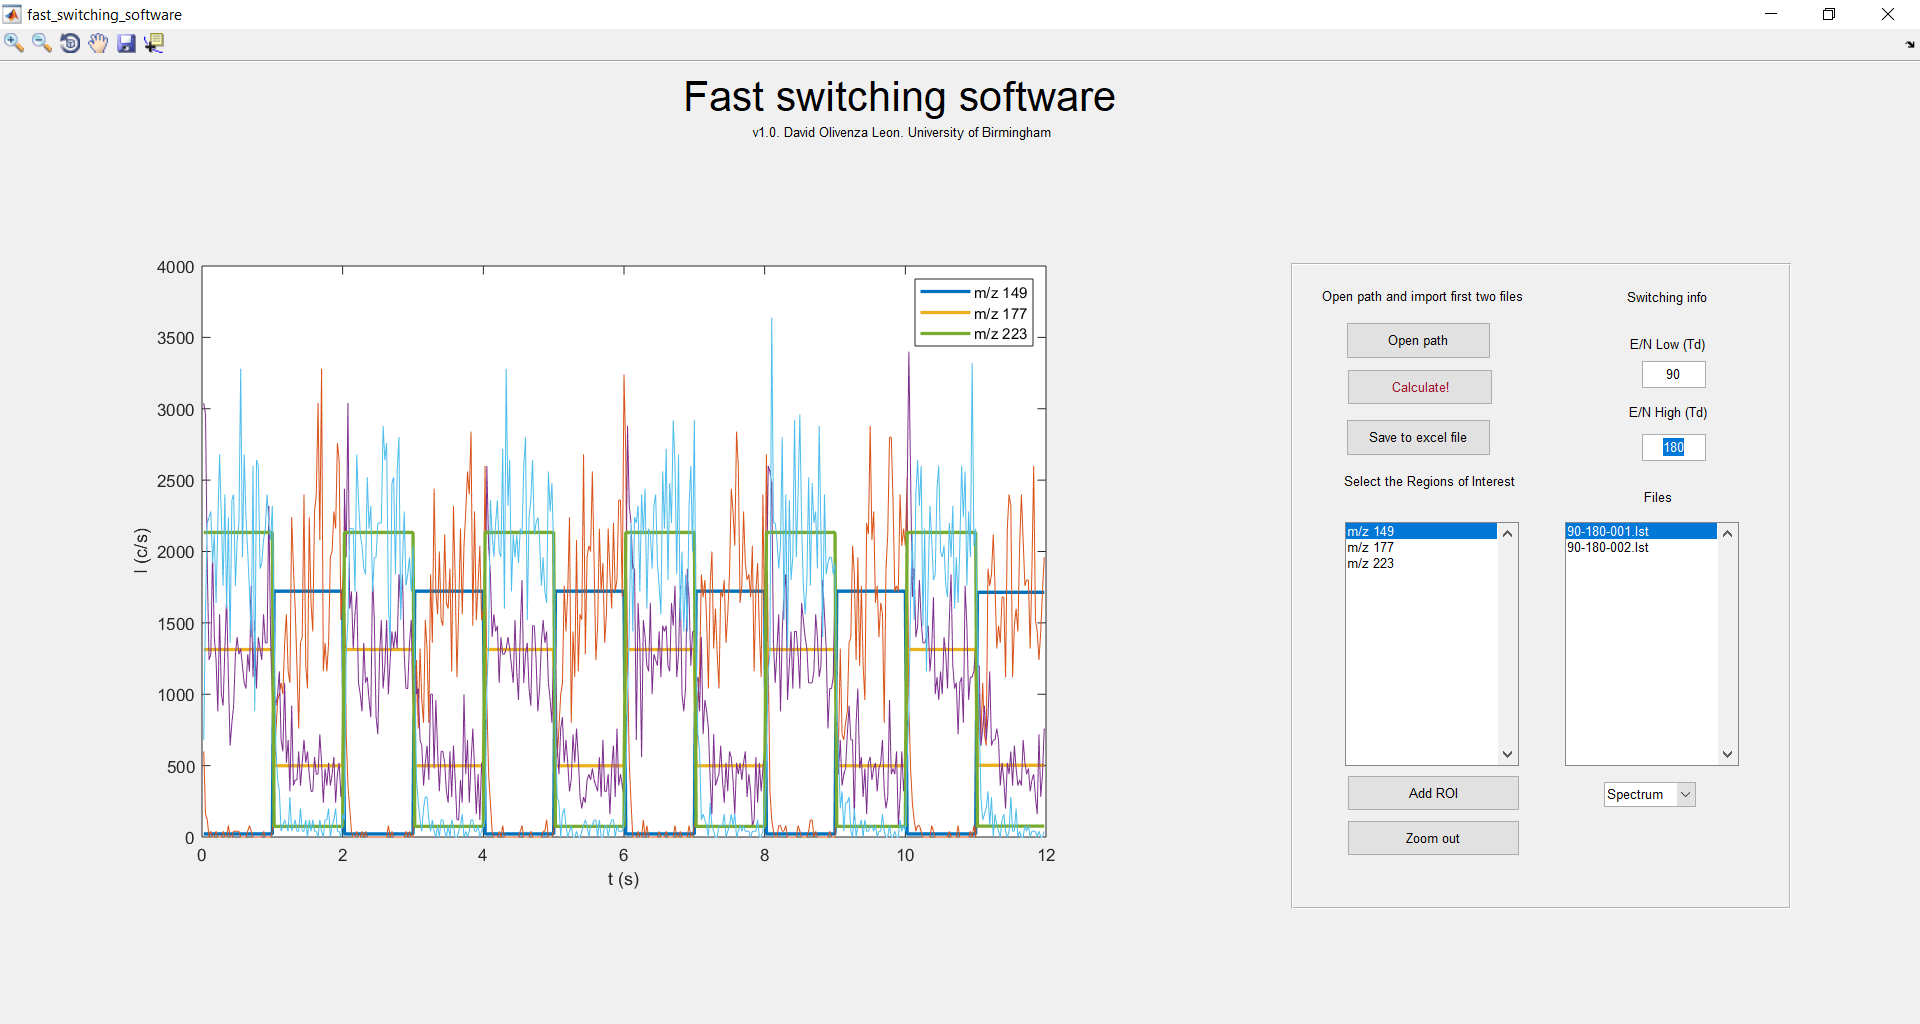
\includegraphics[height=0.4\textheight]{pics/fss.png}}
%\sidesubfloat[]{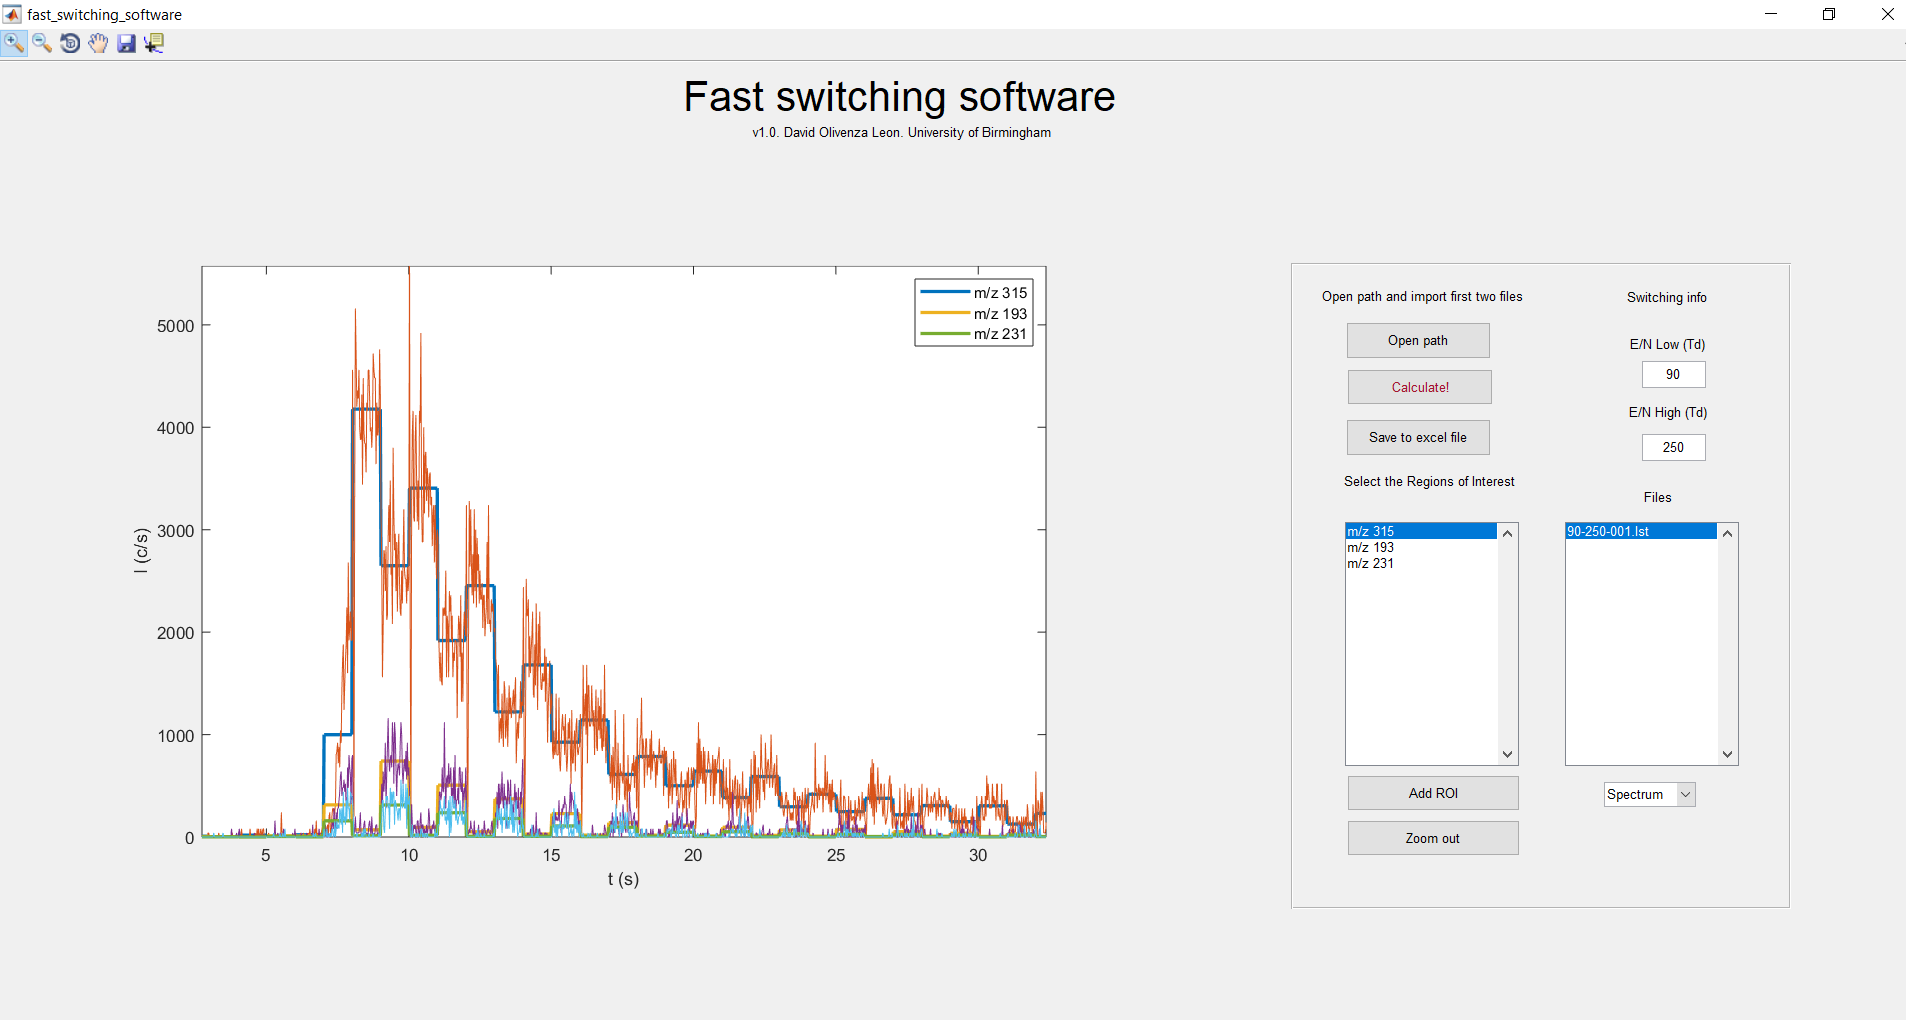
\includegraphics[height=0.4\textheight]{pics/fs_CBD.png}}
\caption[Screenshot of the graphical user interface for the script that  analyses  fast-switching data]{Screenshot of the graphical user interface for the script that  analyses  fast-switching data for: (a)  a steady signal, and (b) a transient experiment.}
\label{fig:fss}
\end{figure}

The files that this script imports are the .lst ones and their accompanying .ini files, which contain the information of the fast switching experiment that is necessary to work with the data.
This  comprehends, among other parameters,
the number of phases,
the number of cycles per phase,
the total number of cycles,
the cycle period,
the number of frames
and
the dead time of the switching.
The number of phases refers to the number of different values that the \textit{E/N} takes during a single experiment. This value is two for the fast switching experiments, which we will refer to as \textit{E/N} low  and \textit{E/N} high.
%
The fast switching frequency is not explicitly recorded but it is given by the inverse of multiplying the cycle period by the number of cycles per phase. For instance, for a cycle period of 40 µs and 25000 cycles per phase, the switching frequency is 1 Hz.
%
The total length of the experiment is not recorded either but, similarly to the switching frequency, it can be calculated by multiplying the cycle period by the total number of cycles. For example, a cycle period of 40 µs and 1.5$\times$10$^6$ total cycles corresponds to a 1 minute experiment.
%
%
%Each of the time intervals in which the drift tube is kept at the same \textit{E/N} is called a frame. 
In a measurement lasting 60 seconds at a fast switching frequency of 1 Hz there are 60 total frames and 30 frames per phase.
%
%
The dead time recorded in the .ini file in this case refers to that given by the delay in the electronics to supply the right voltage to the drift tube (i.e. the rise and fall times) and it is around 70 ms. The software automatically ignores the interval three times bigger than this dead time to account for the capacitance of the reactor, which was explained  in section \ref{section:fs}.
%Phases = 2
%Frames = 30
%Cycle period us=40
%Number of cycles=1500000
%Phases=2
%Cycles per phase=25000
%Frames=30
%Dead time ms=70




If the files are saved with the name format [\textit{low E/N}]-[\textit{high E/N}]-[\textit{file number}], the script automatically reads and writes in the output file the values of the low and high \textit{E/N}. If not, they must be manually added.
%
The data inside each frame can be exported in raw format or averaged.
For steady experiments like the one shown in \autoref{fig:fss}(a), the data from all the frames from a phase (i.e. high or low \textit{E/N}) can also be averaged like it is shown in this figure. Obviously, this does not make sense for transient measurements like that in \autoref{fig:fss}(b).
%
Once the data analysis is finished, the results can be exported. The format these files are saved at allows easy double-y axis plot of the ion intensities and \textit{E/N} as a function of the experiment time, as it is shown in \autoref{fig:fss_plots}, for a (a,c) steady-state  and (b,d) transient measurement.




\begin{figure}[t]
\centering
\sidesubfloat[]{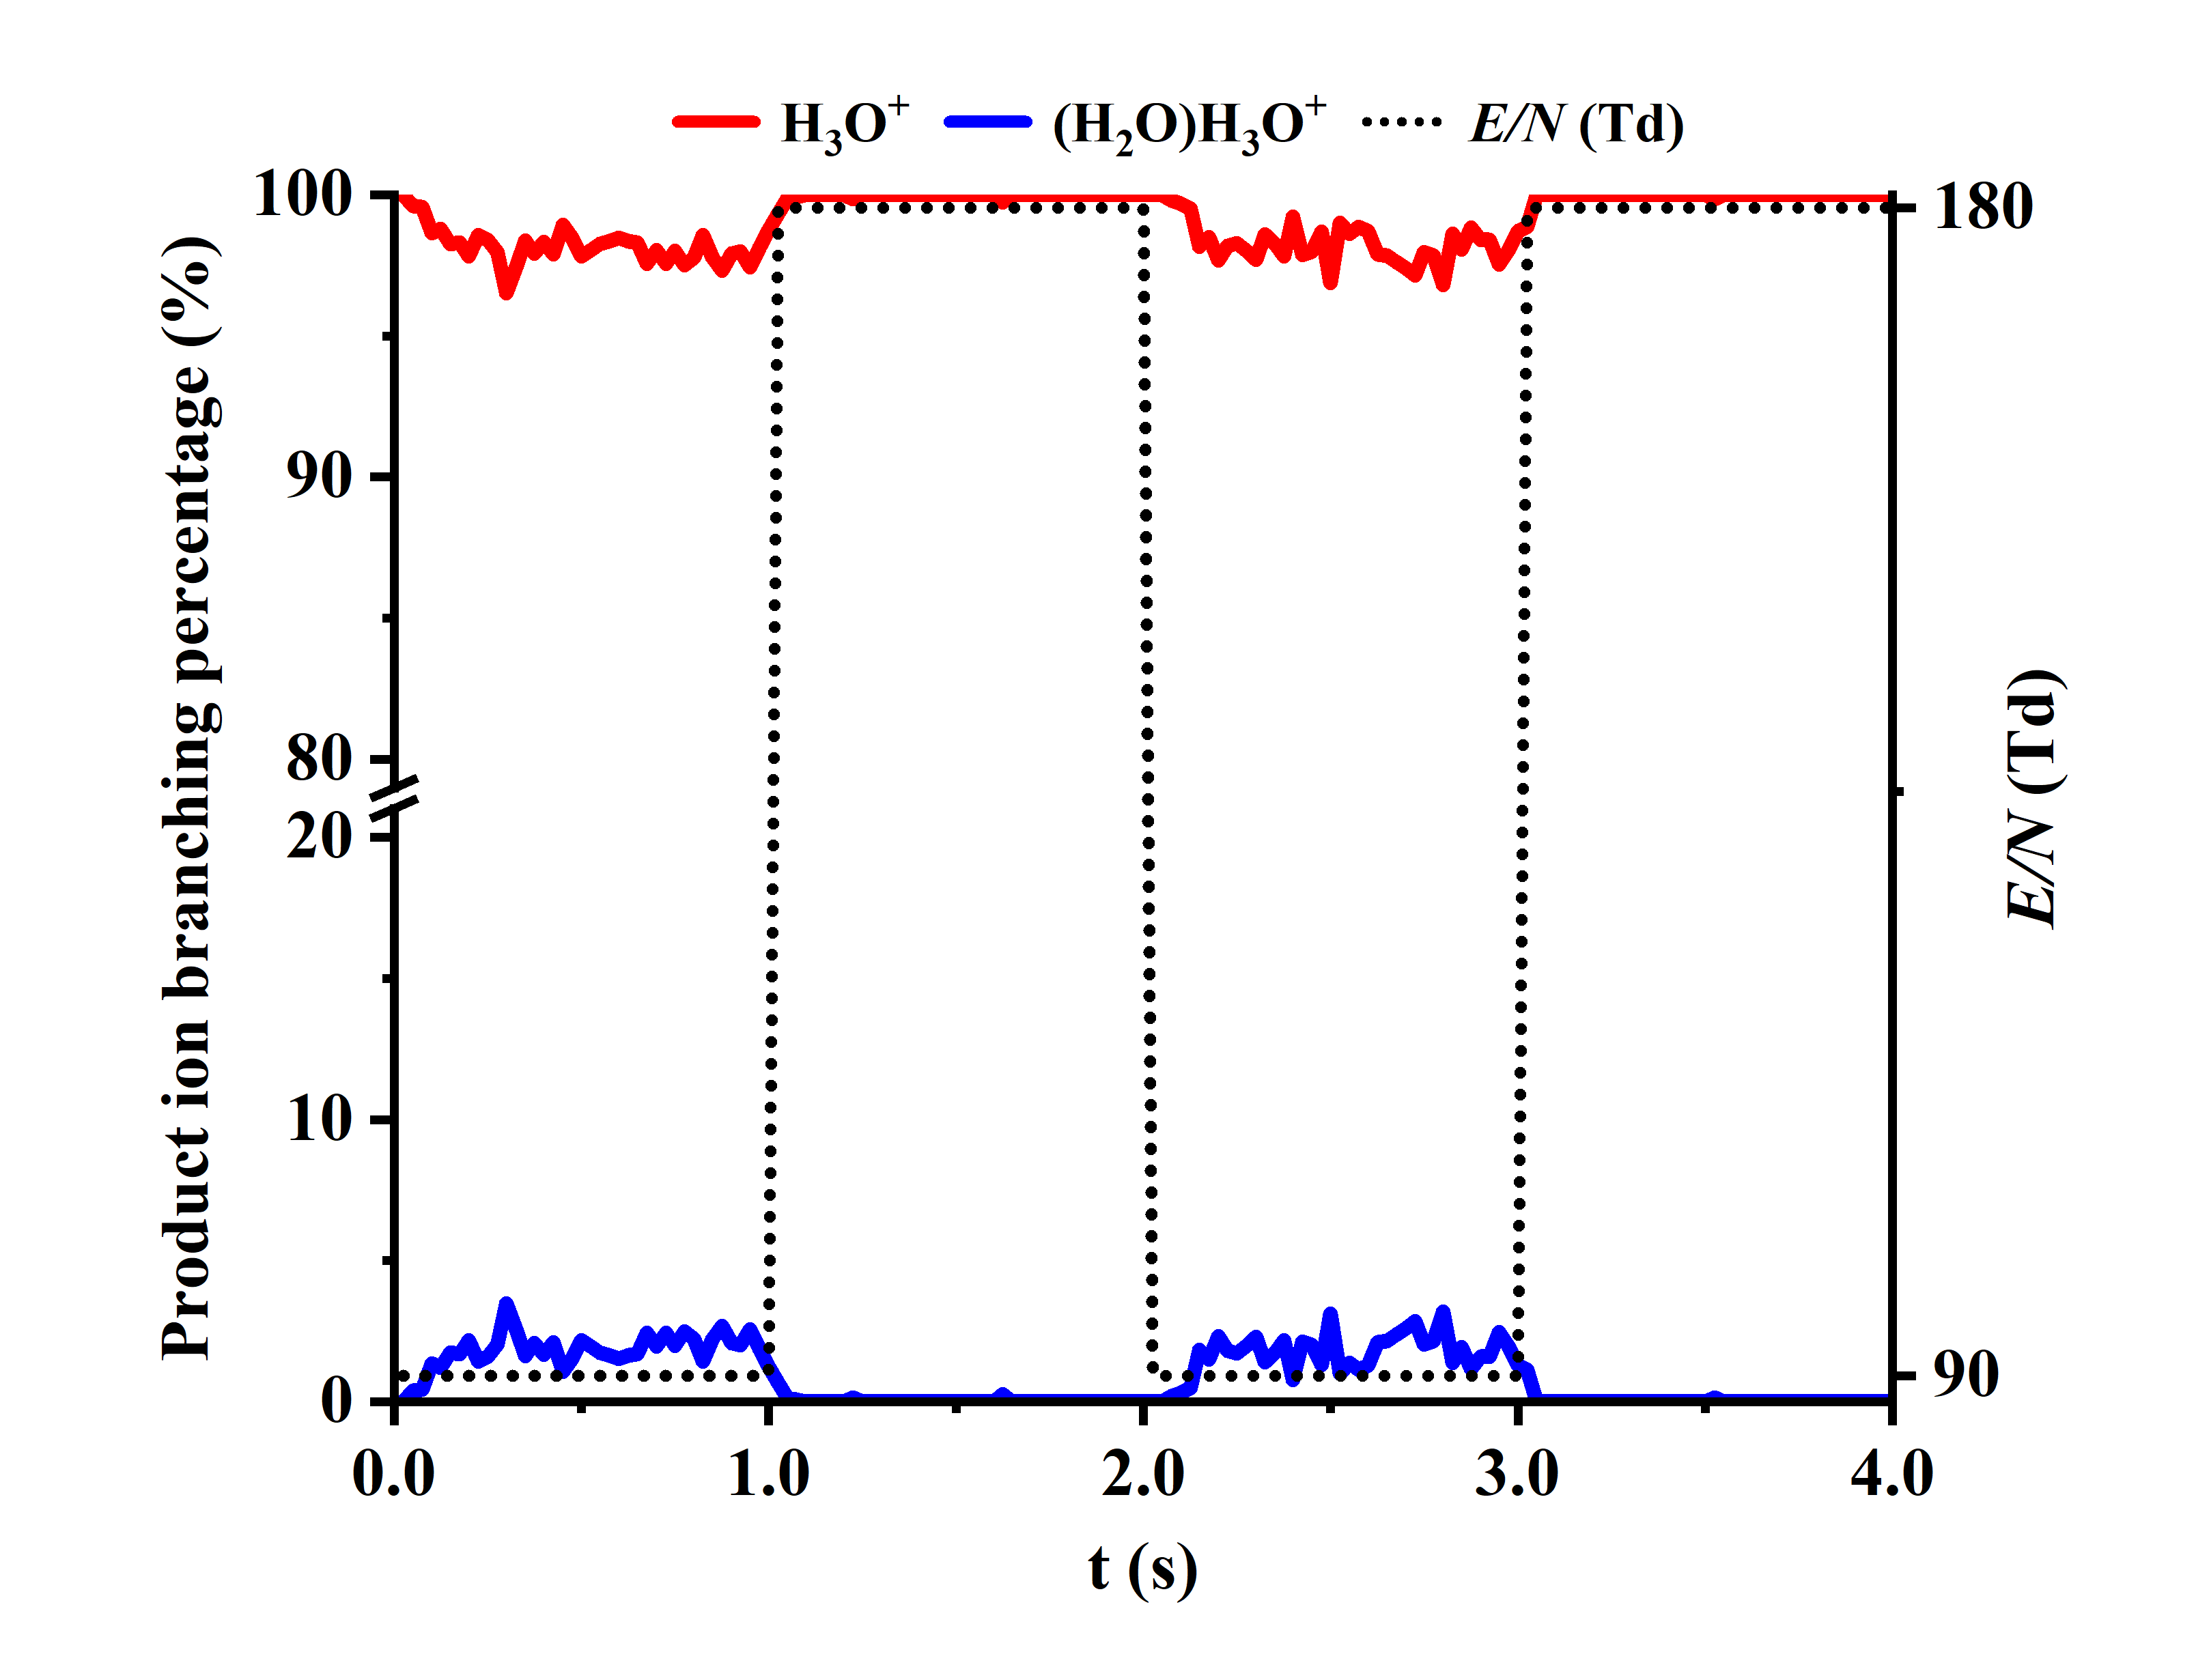
\includegraphics[width=0.45\textwidth]{pics/RIDPM90180Td.png}}
\sidesubfloat[]{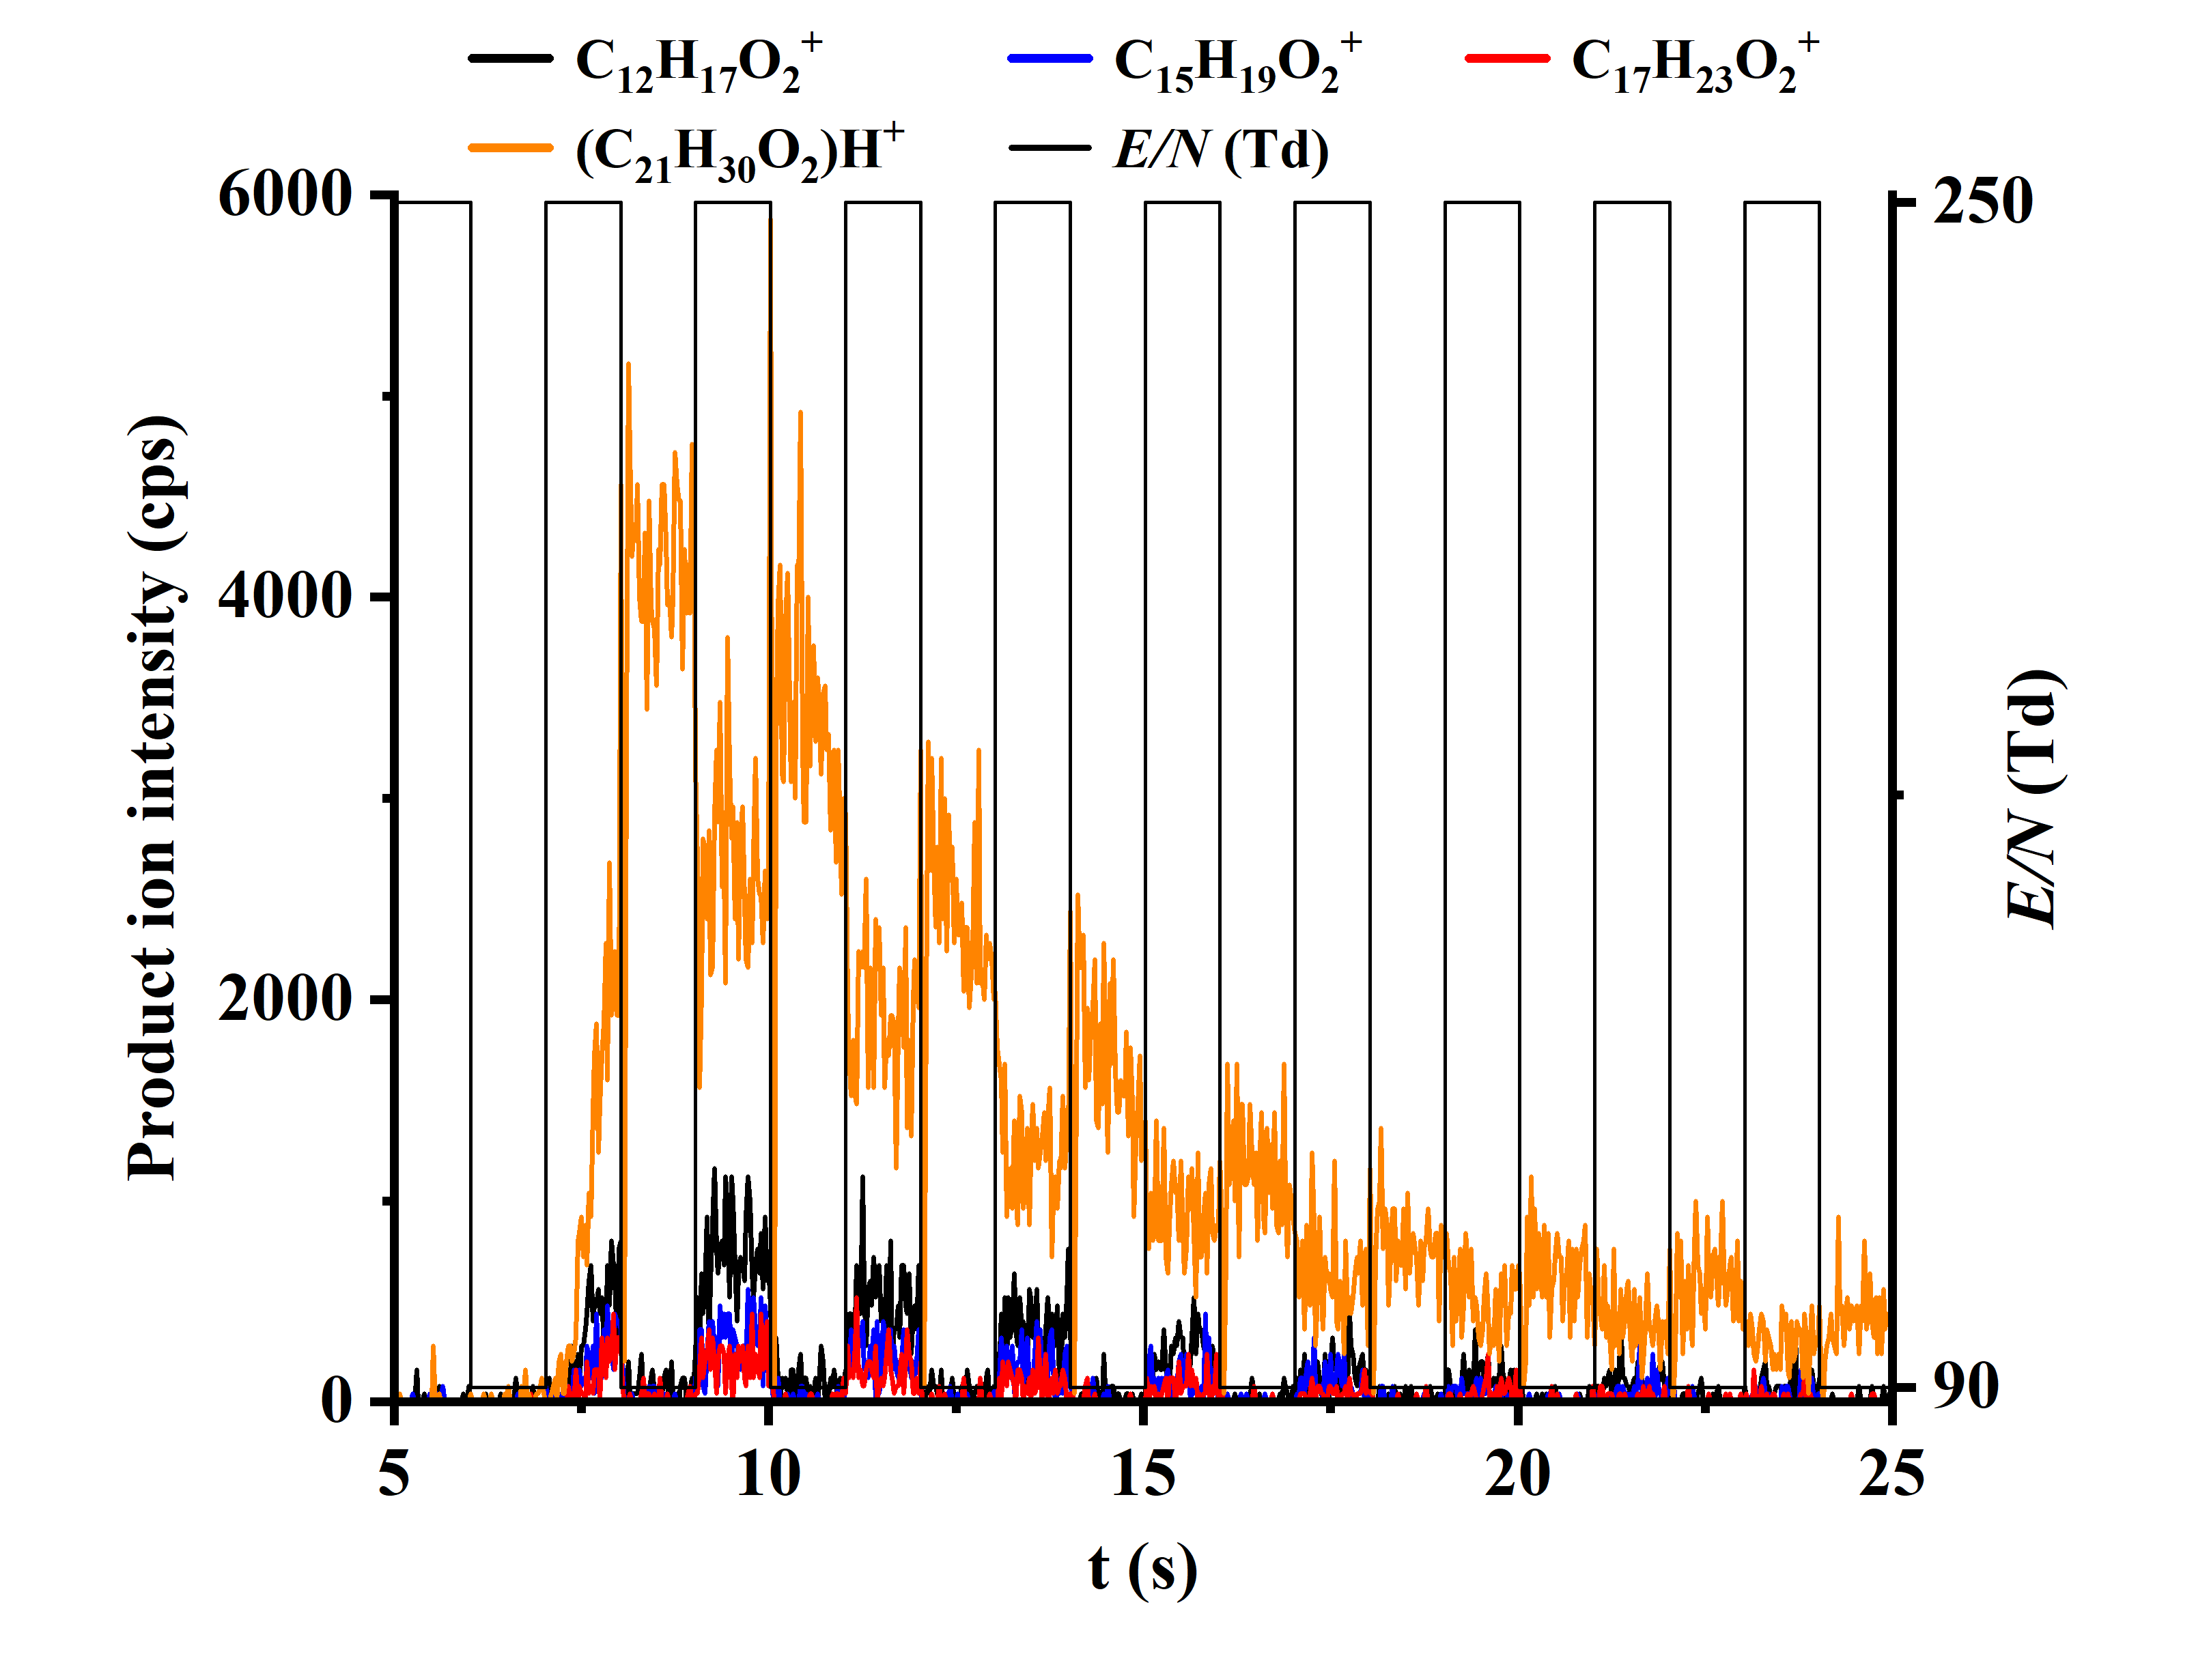
\includegraphics[width=0.45\textwidth]{pics/CBD-raw.png}}

\sidesubfloat[]{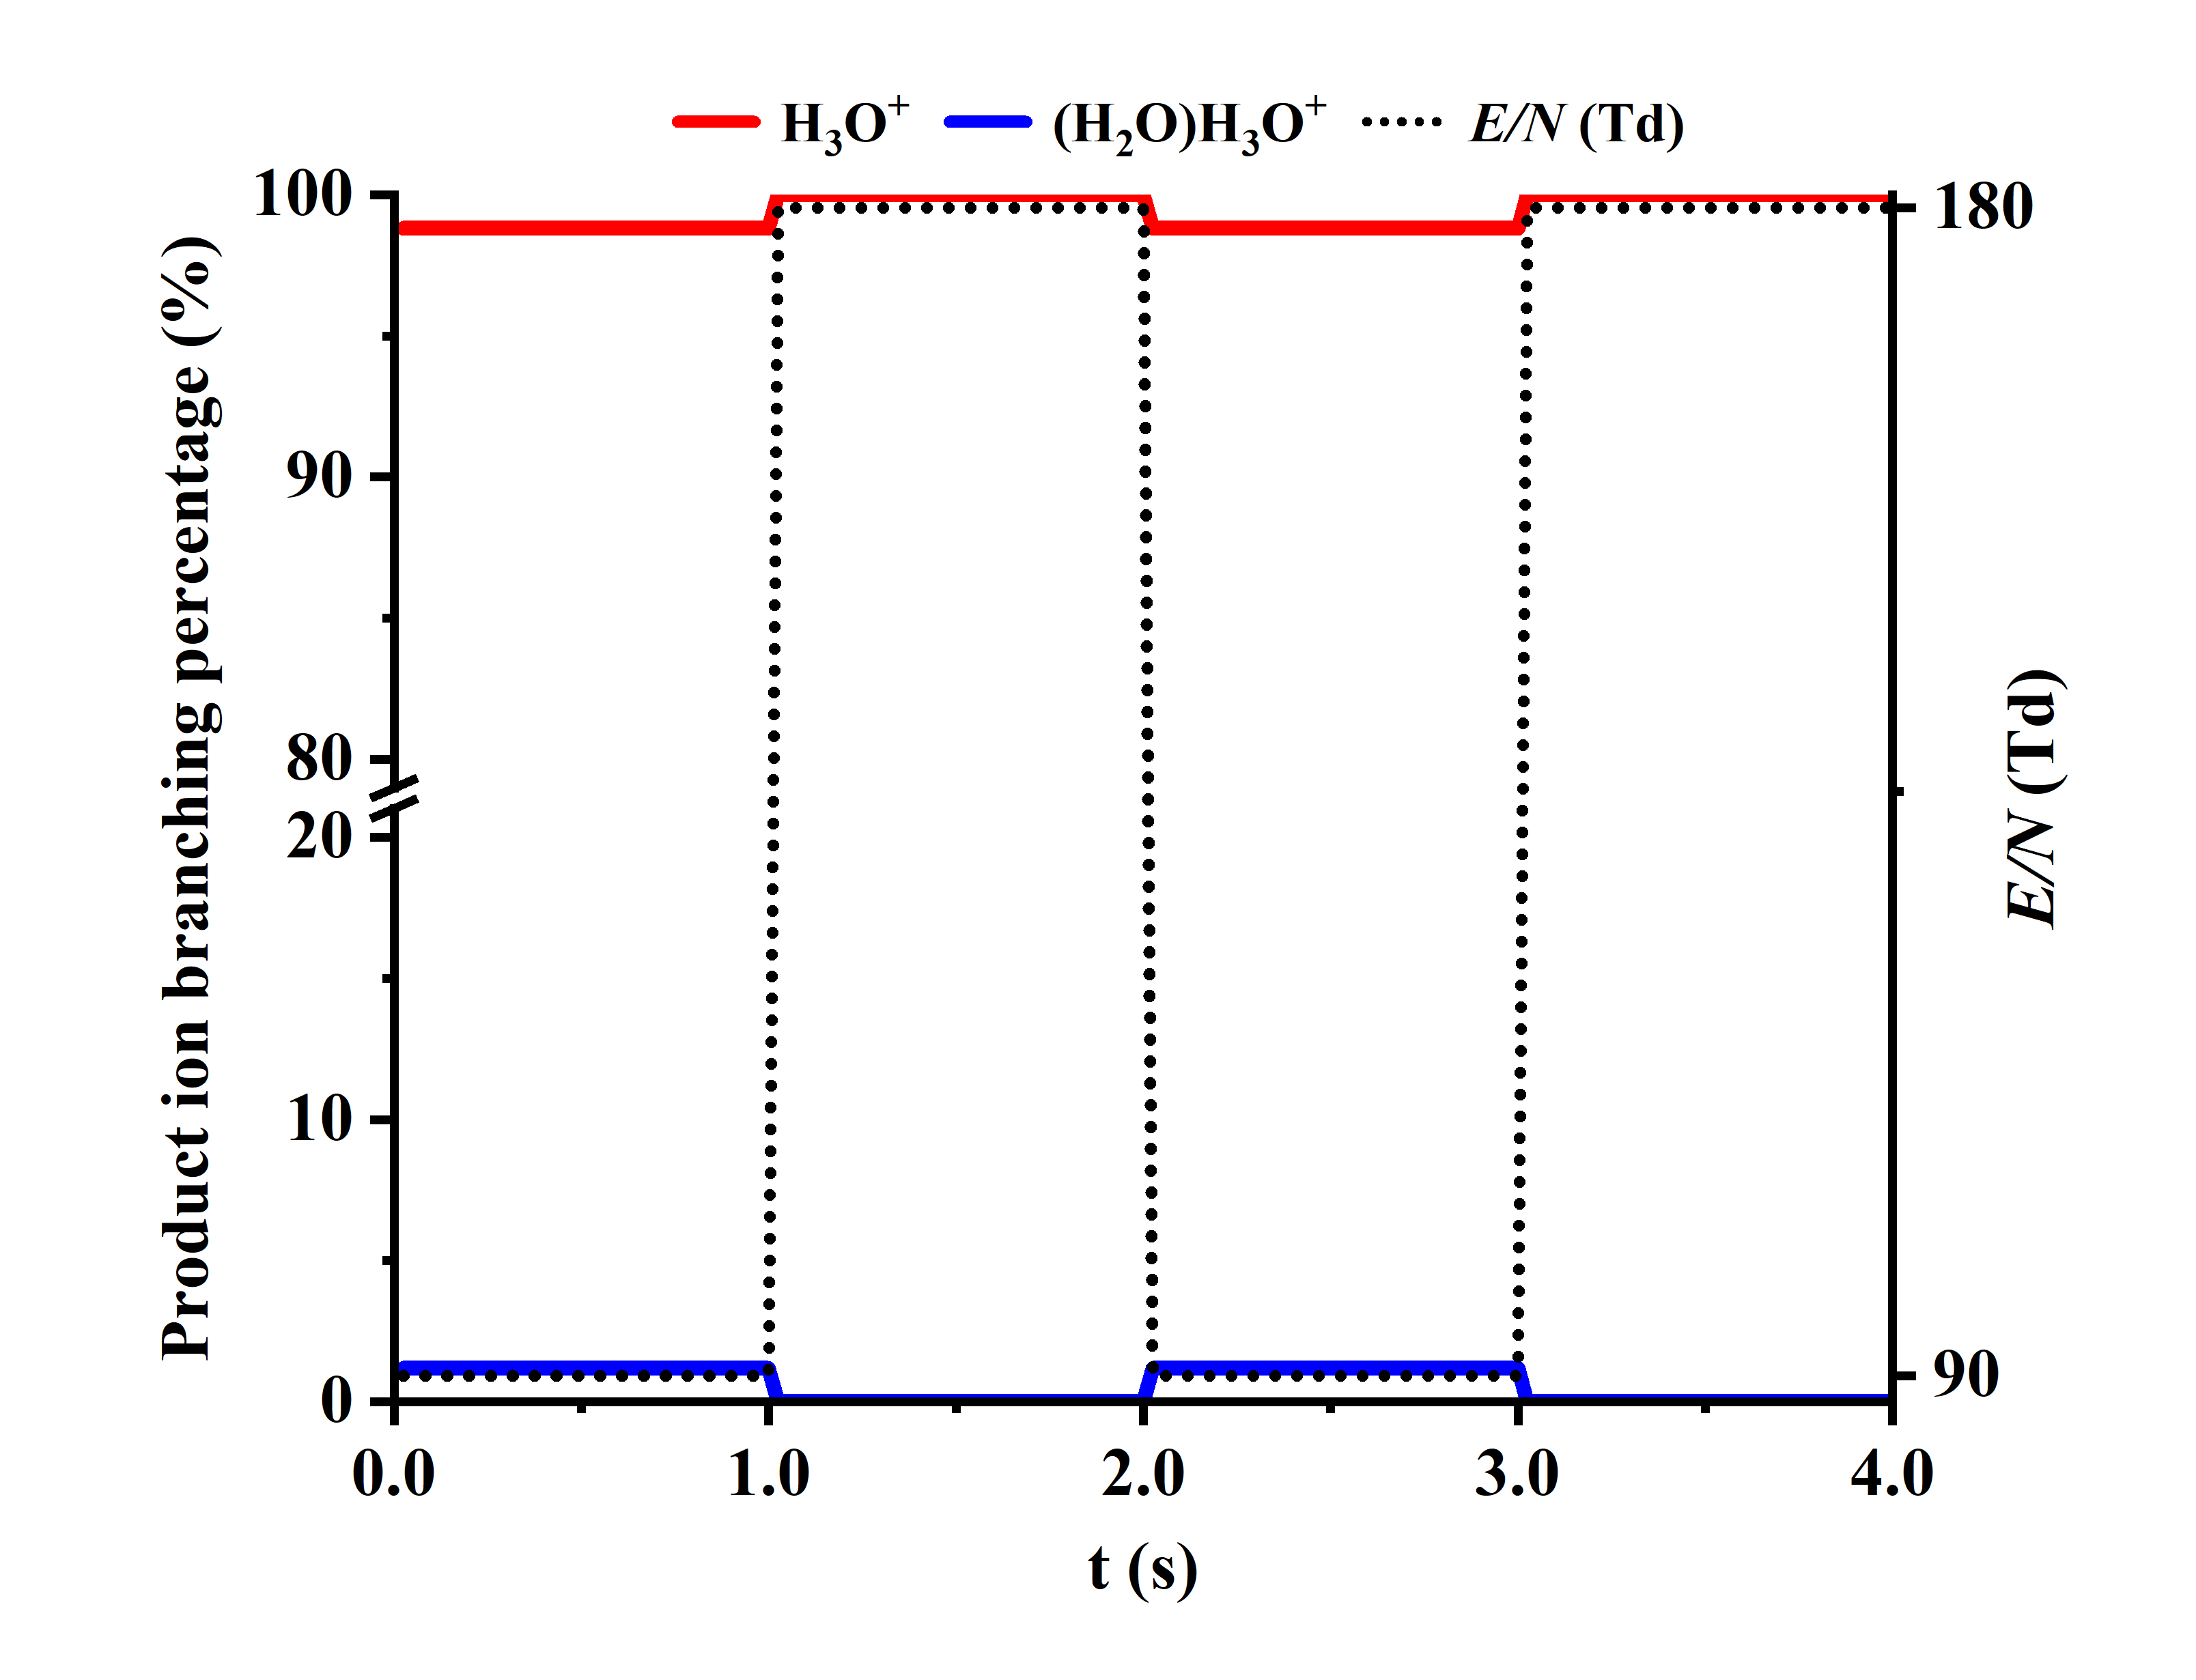
\includegraphics[width=0.45\textwidth]{pics/RIDPM90180Td-averaged.png}}
\sidesubfloat[]{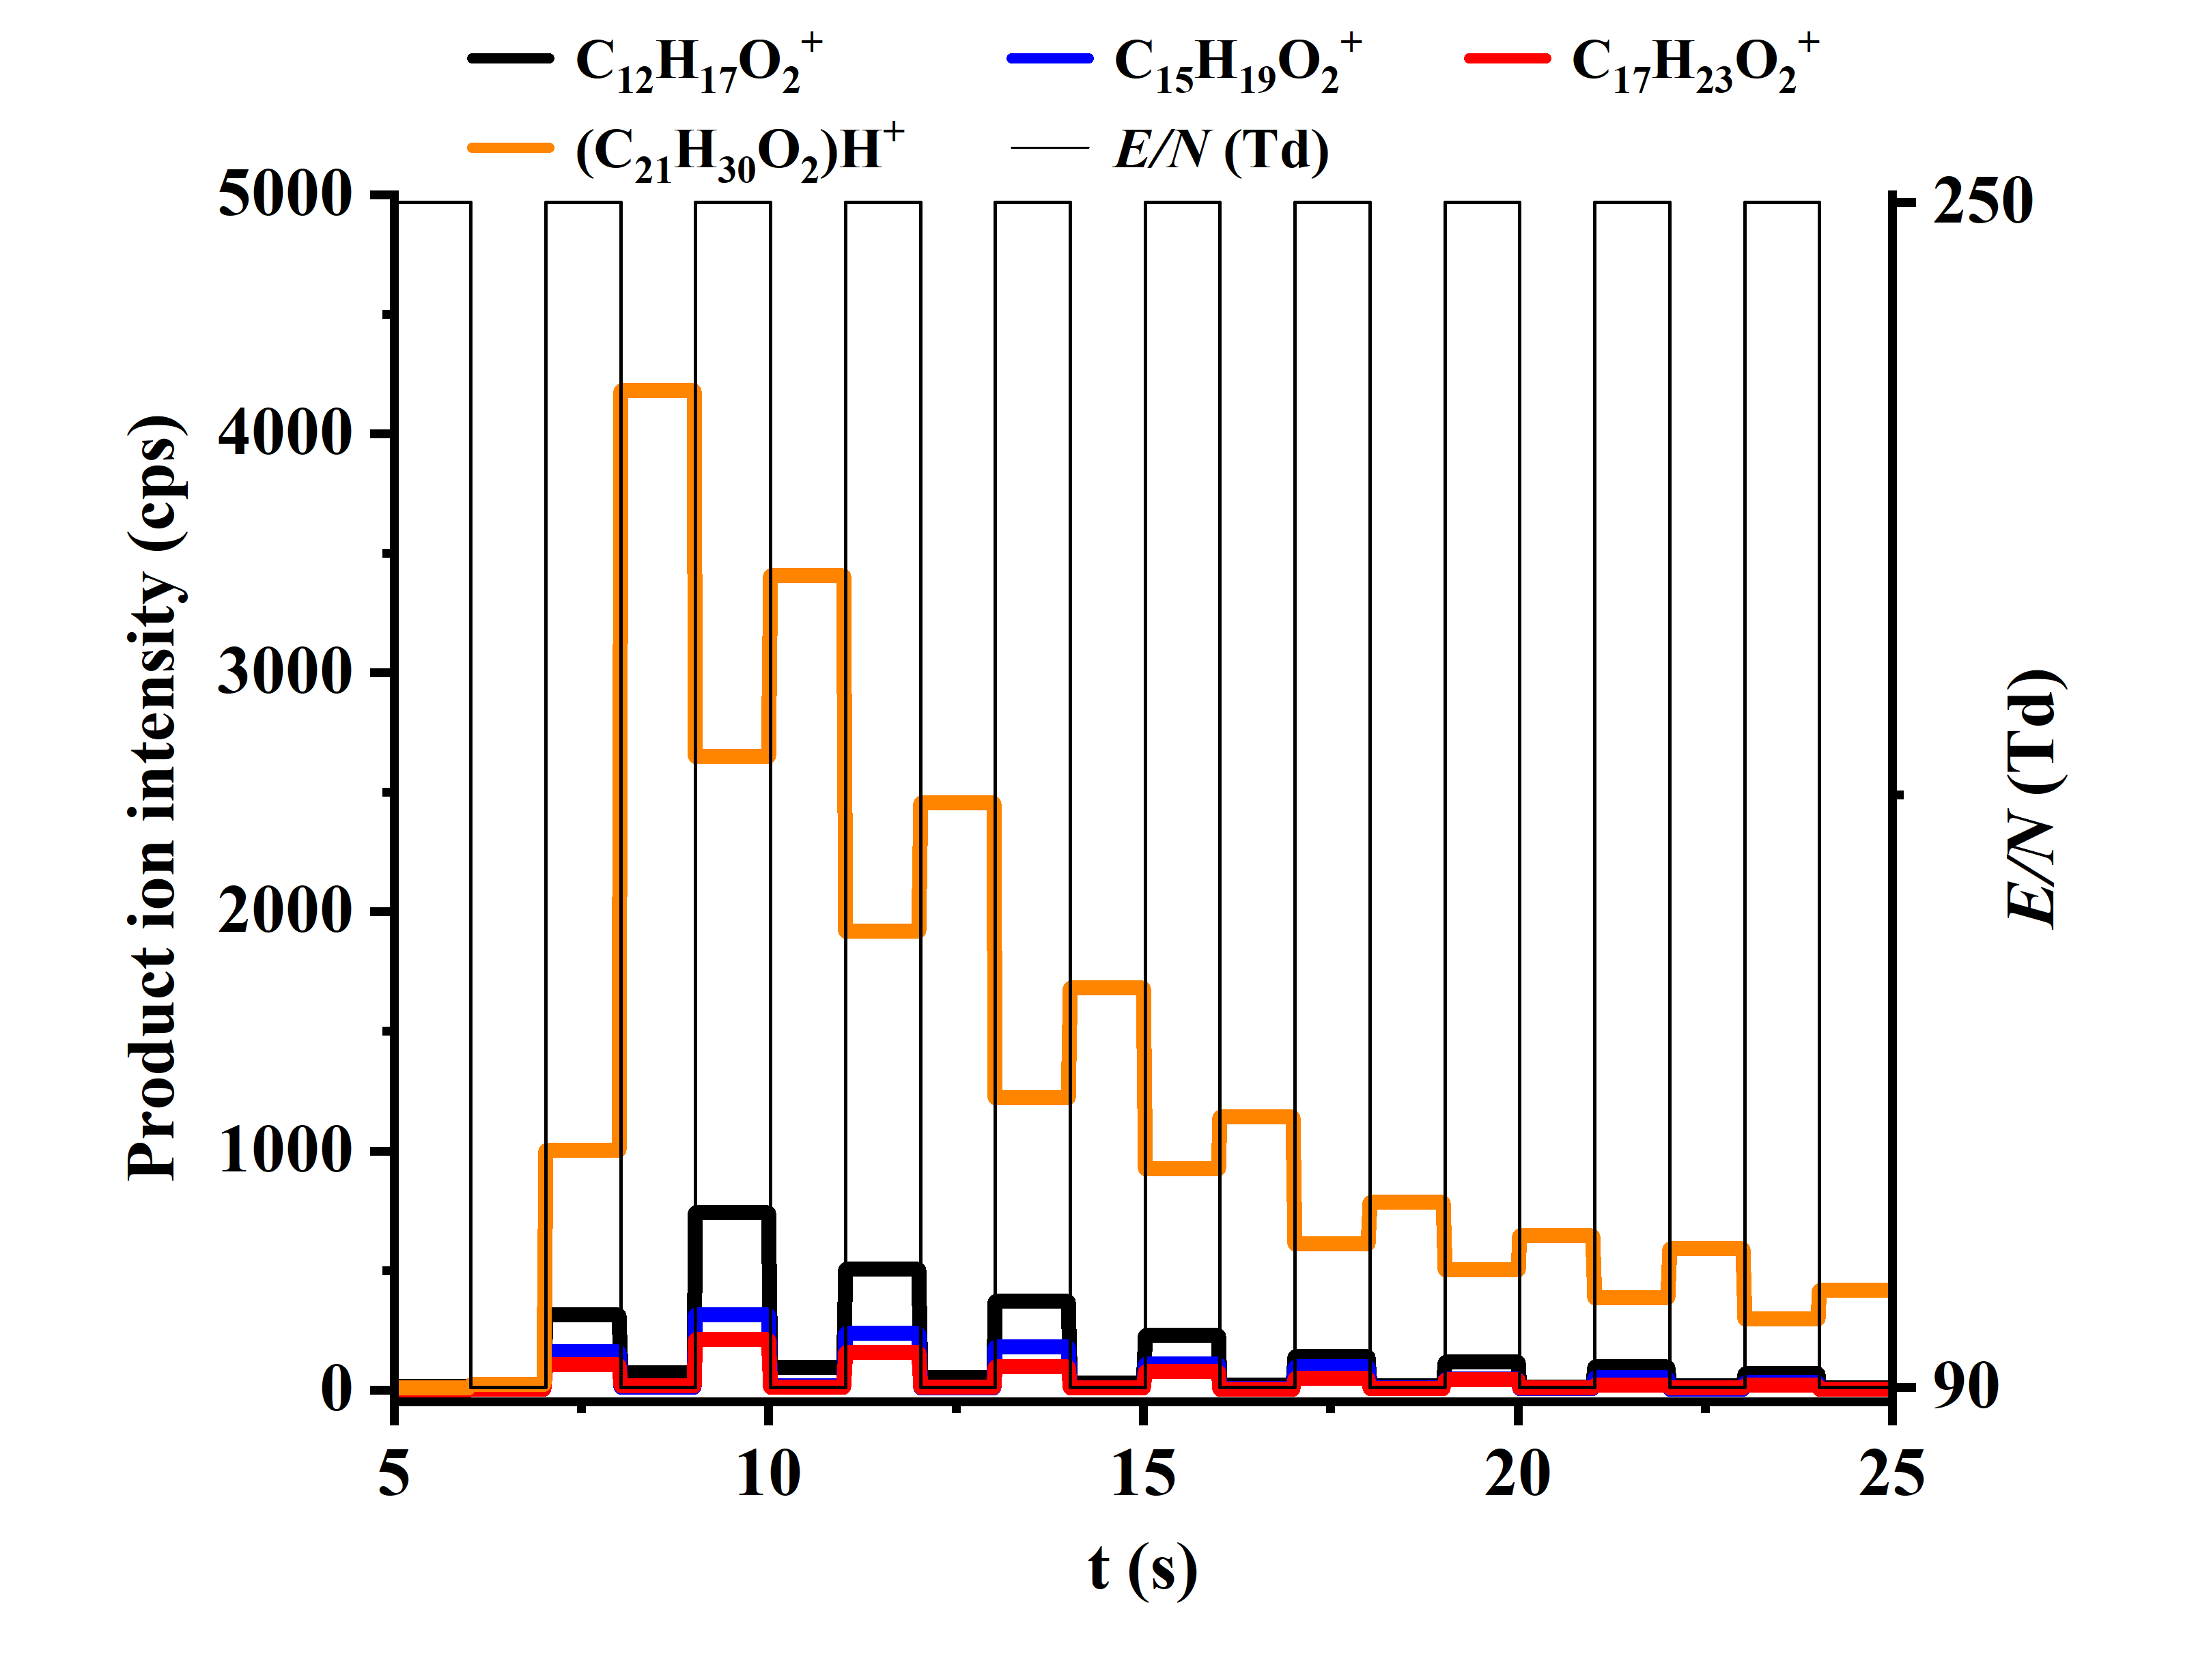
\includegraphics[width=0.45\textwidth]{pics/CBD-raw2.png}}
\caption[Example plots of data analysed with the fast-switching software]{Example plots of data analysed with the fast-switching software. Left: (a) raw and (c) averaged plots of H$_3$O$^+$ and (H$_2$O)H$_3$O$^+$ for the fast switching between 90 and 180 Td. Right: (b) raw and (d) averaged plots of the signal obtained from the desorption of trace amounts of cannabidiol while fast switching the reduced electric field between 90 and 250 Td.}
\label{fig:fss_plots}
\end{figure}


\subsection{Density functional theory}
Experimental data in this thesis is in some cases accompanied by theoretical values of the proton affinity, gas-phase basicity and energetics of the protonation and/or fragmentation reactions.
These density functional theory (\acrshort{dft}) results were computed   by Dr Peter Watts using  
Gaussian09W and GaussView05 for Windows  and the B3LYP functional with the 6-31+G(d,p) basis set  \cite{frisch2009gaussian}.

%\subsubsection{Saturation: Poisson distribution}

%The counting electronics in the PTR-ToF-MS assumes that each pulse measured at the MCP corresponds to one ion. This can be not true if two or more ions arrive at the detector very close together and their analogue signals overlap so that the TDC translates it as a single event. This is known as saturation and happens more often when a high concentration of a compound is being measured.

%At a given m/z, the maximum number of counts per second the instrument can measure corresponds to the number of cycles per second of the mass spectrometer, which is the number of times the ions are pulsed per second. In other words, at a certain \textit{m/z} only one ion per cycle can be measured. Therefore, a compromise must be found when the experiment is being designed to avoid situations of saturation while getting a proper signal. The number of cycles is the inverse of the cycle time, which is usually 30 to 40 us. For example, for a cycle time of 30 us, the number of cycles per second is 33333, or in other words, the pulsing frequency is 33.333 kHz.

%\autoref{fig:sat} shows the difference in real and measured counts if the probability of two ions arriving at the detector at the same time is given by the Poisson distribution function and considering that saturation means more than one ion arriving at the same time. When we are measuring a number of events equal to the number of cycles per second is unlikely that only one ion is arriving at the detector at a time, and the signal is highly saturated.

%The analytical expression is:
%\begin{equation}
%\label{eq:sat}
%P(x) = 1 - e^{-x}
%\end{equation}


%\begin{figure}%[ht]
%\centering
%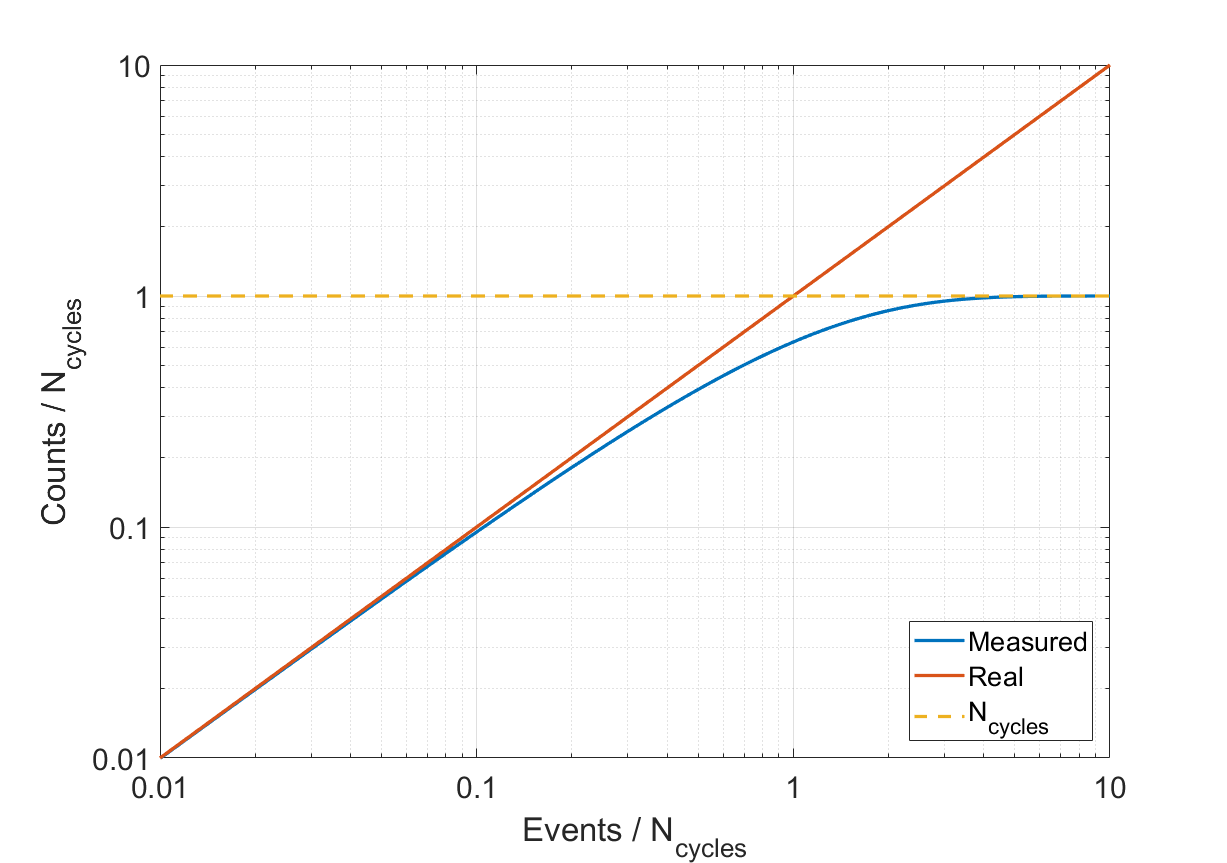
\includegraphics[width=0.8\linewidth]{pics/saturation.png}
%\centering
%\caption[Plot of the measured and real counts as a function of the number of events per cycle of the mass spectrometer.]{Plot of the measured (blue) and real (red) counts as a function of the number of events per cycle of the mass spectrometer. The dashed line corresponds to the number of cycles per second and indicates the maximum possible measured counts. Note that this plot is normalised to the number of cycles per second.}
%\label{fig:sat}
%\end{figure}




\section{PTR-MS Add-ons}
%\section{PTR-MS add-ons and latest hardware developments}
Besides the essential components described  earlier in this chapter, there are some accessories that can be coupled to a PTR-MS instrument for different purposes.
These include devices  like the CHARON real-time aerosol inlet  or the PREFICS pre concentrator with chromatographic separation \cite{muller2017direct,piel2019airborne,prefics}.
The ones included in this section are those used at some point for the experimental work in this thesis.




\subsection{Thermal Desorption Unit}\label{section:tdu}
For many applications, PTR-MS has been demonstrated to be a sensitive tool, yet the primary method for homeland security applications is \acrshort{ims}.
%
Most substances of relevance in this sector, including drugs and explosives, as well as in other fields have a small vapour pressure at room temperature, which challenges their identification. These are often referred to as semi-volatile organic compounds (\acrshort{svoc}s).
%
The sampling method is then critical in the detection of traces ammounts of these substances.


This issue has been approached in many interesting ways.
%
These include the patents for hand-held suction systems capable of identifying small quantities of explosives that were granted to \citeauthor{conrad1992hand} and to \citeauthor{carroll1992hand} \cite{conrad1992hand,carroll1992hand}.
%
\citeauthor{jjunju2015hand} also created a portable tool to detect nitroaromatic explosives on-site via atmospheric pressure chemical ionisation that can operate for 12 h in one charge \cite{jjunju2015hand}.
%
Additionally, the development of a biomimetic electronic dog nose by \citeauthor{staymates2016biomimetic} is an exciting new development \cite{staymates2016biomimetic}.
%Similar approaches to that mentioned here are taken by \citeauthor{ebejer2005rapid} \cite{ebejer2005rapid}



Swab desorptions are commonly used in  IMS  and the same approach can be brought into PTR-MS.
%
A thermal desorption unit (\acrshort{tdu})  like that engineered by KORE Technology Ltd  can be used to study SVOCs when coupled to a PTR-MS device (\autoref{fig:tdu}).
%
This was applied by \citeauthor{RN445} to the detection of explosives %reaching limits of detection (\acrshort{lod}) of nanograms  
and by \citeauthor{blenkhorn2019novel} to the detection polyaromatic hydrocarbons \cite{RN445,blenkhorn2019novel}.
%
This TDU works with polytetrafluoroethylene (\acrshort{ptfe}) swabs (ThermoFisher Scientific, Cheshire, UK) mounted in a cardboard frame (shown in \autoref{fig:tdu}(a)) onto which the targeted compounds are deposited.
%
Then, the swab is inserted in the TDU, whose plates come together clamping the swab and creating a high-quality circular seal. The metal plates are kept at high temperature (150$^{\circ}$C) and a carrier gas is flown through their holes, pulling the analyte towards the inlet pipe, whose surfaces are passivated (treated with SilcoNert\textsuperscript{\textregistered} 2000) to minimise adsorption.
%
This creates a desorption profile like the one in \autoref{fig:tdu_heroin}, where the two main fragment ions from trace amounts of the desorption of heroin are shown.
%
The duration of the desorption depends on many factors, being some of them the volatility of the analyte, the temperature of the inlet and TDU and the carrier gas flow.
%
The ion signal goes down to 10\% of the peak maximum in between 10 to 20 seconds, although
it usually takes between 60 and 120 seconds for a sample to be completely desorbed into the instrument (i.e. to reach baseline) after the swab has been inserted in the TDU and its jaws have clamped together. 
%
After the measurement is finished, the TDU can be opened to extract the swab, which can be reused.







%\cite{koretdu}

\begin{figure}%[t]
  \sidesubfloat[]{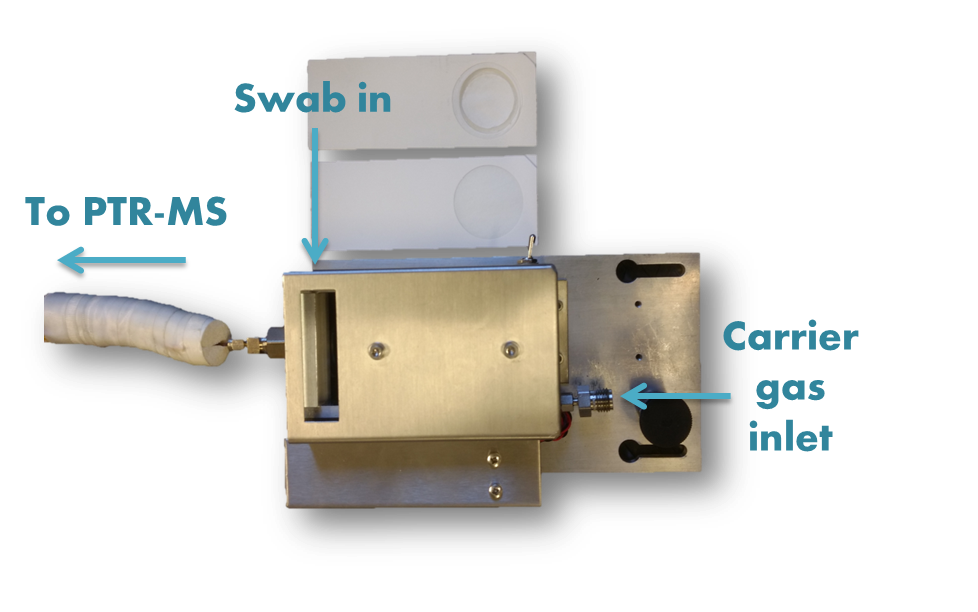
\includegraphics[width=0.7\linewidth]{pics/tdu.png}\label{fig:tdu1}}\\
  \sidesubfloat[]{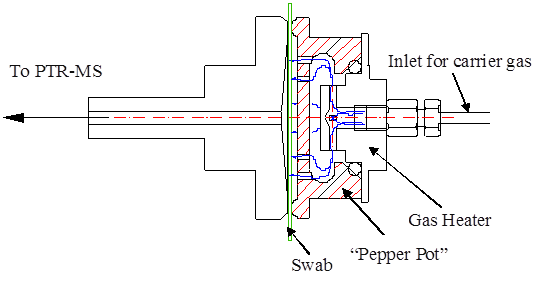
\includegraphics[width=0.7\linewidth]{pics/tdu2.png}\label{fig:tdu2}}
  \caption{(a) Picture of the TDU near to (top) used and (bottom) new PTFE swabs. (b) Schematic diagram of the TDU \cite{RN445}.}\label{fig:tdu}
\end{figure}

\begin{figure}%[t]
  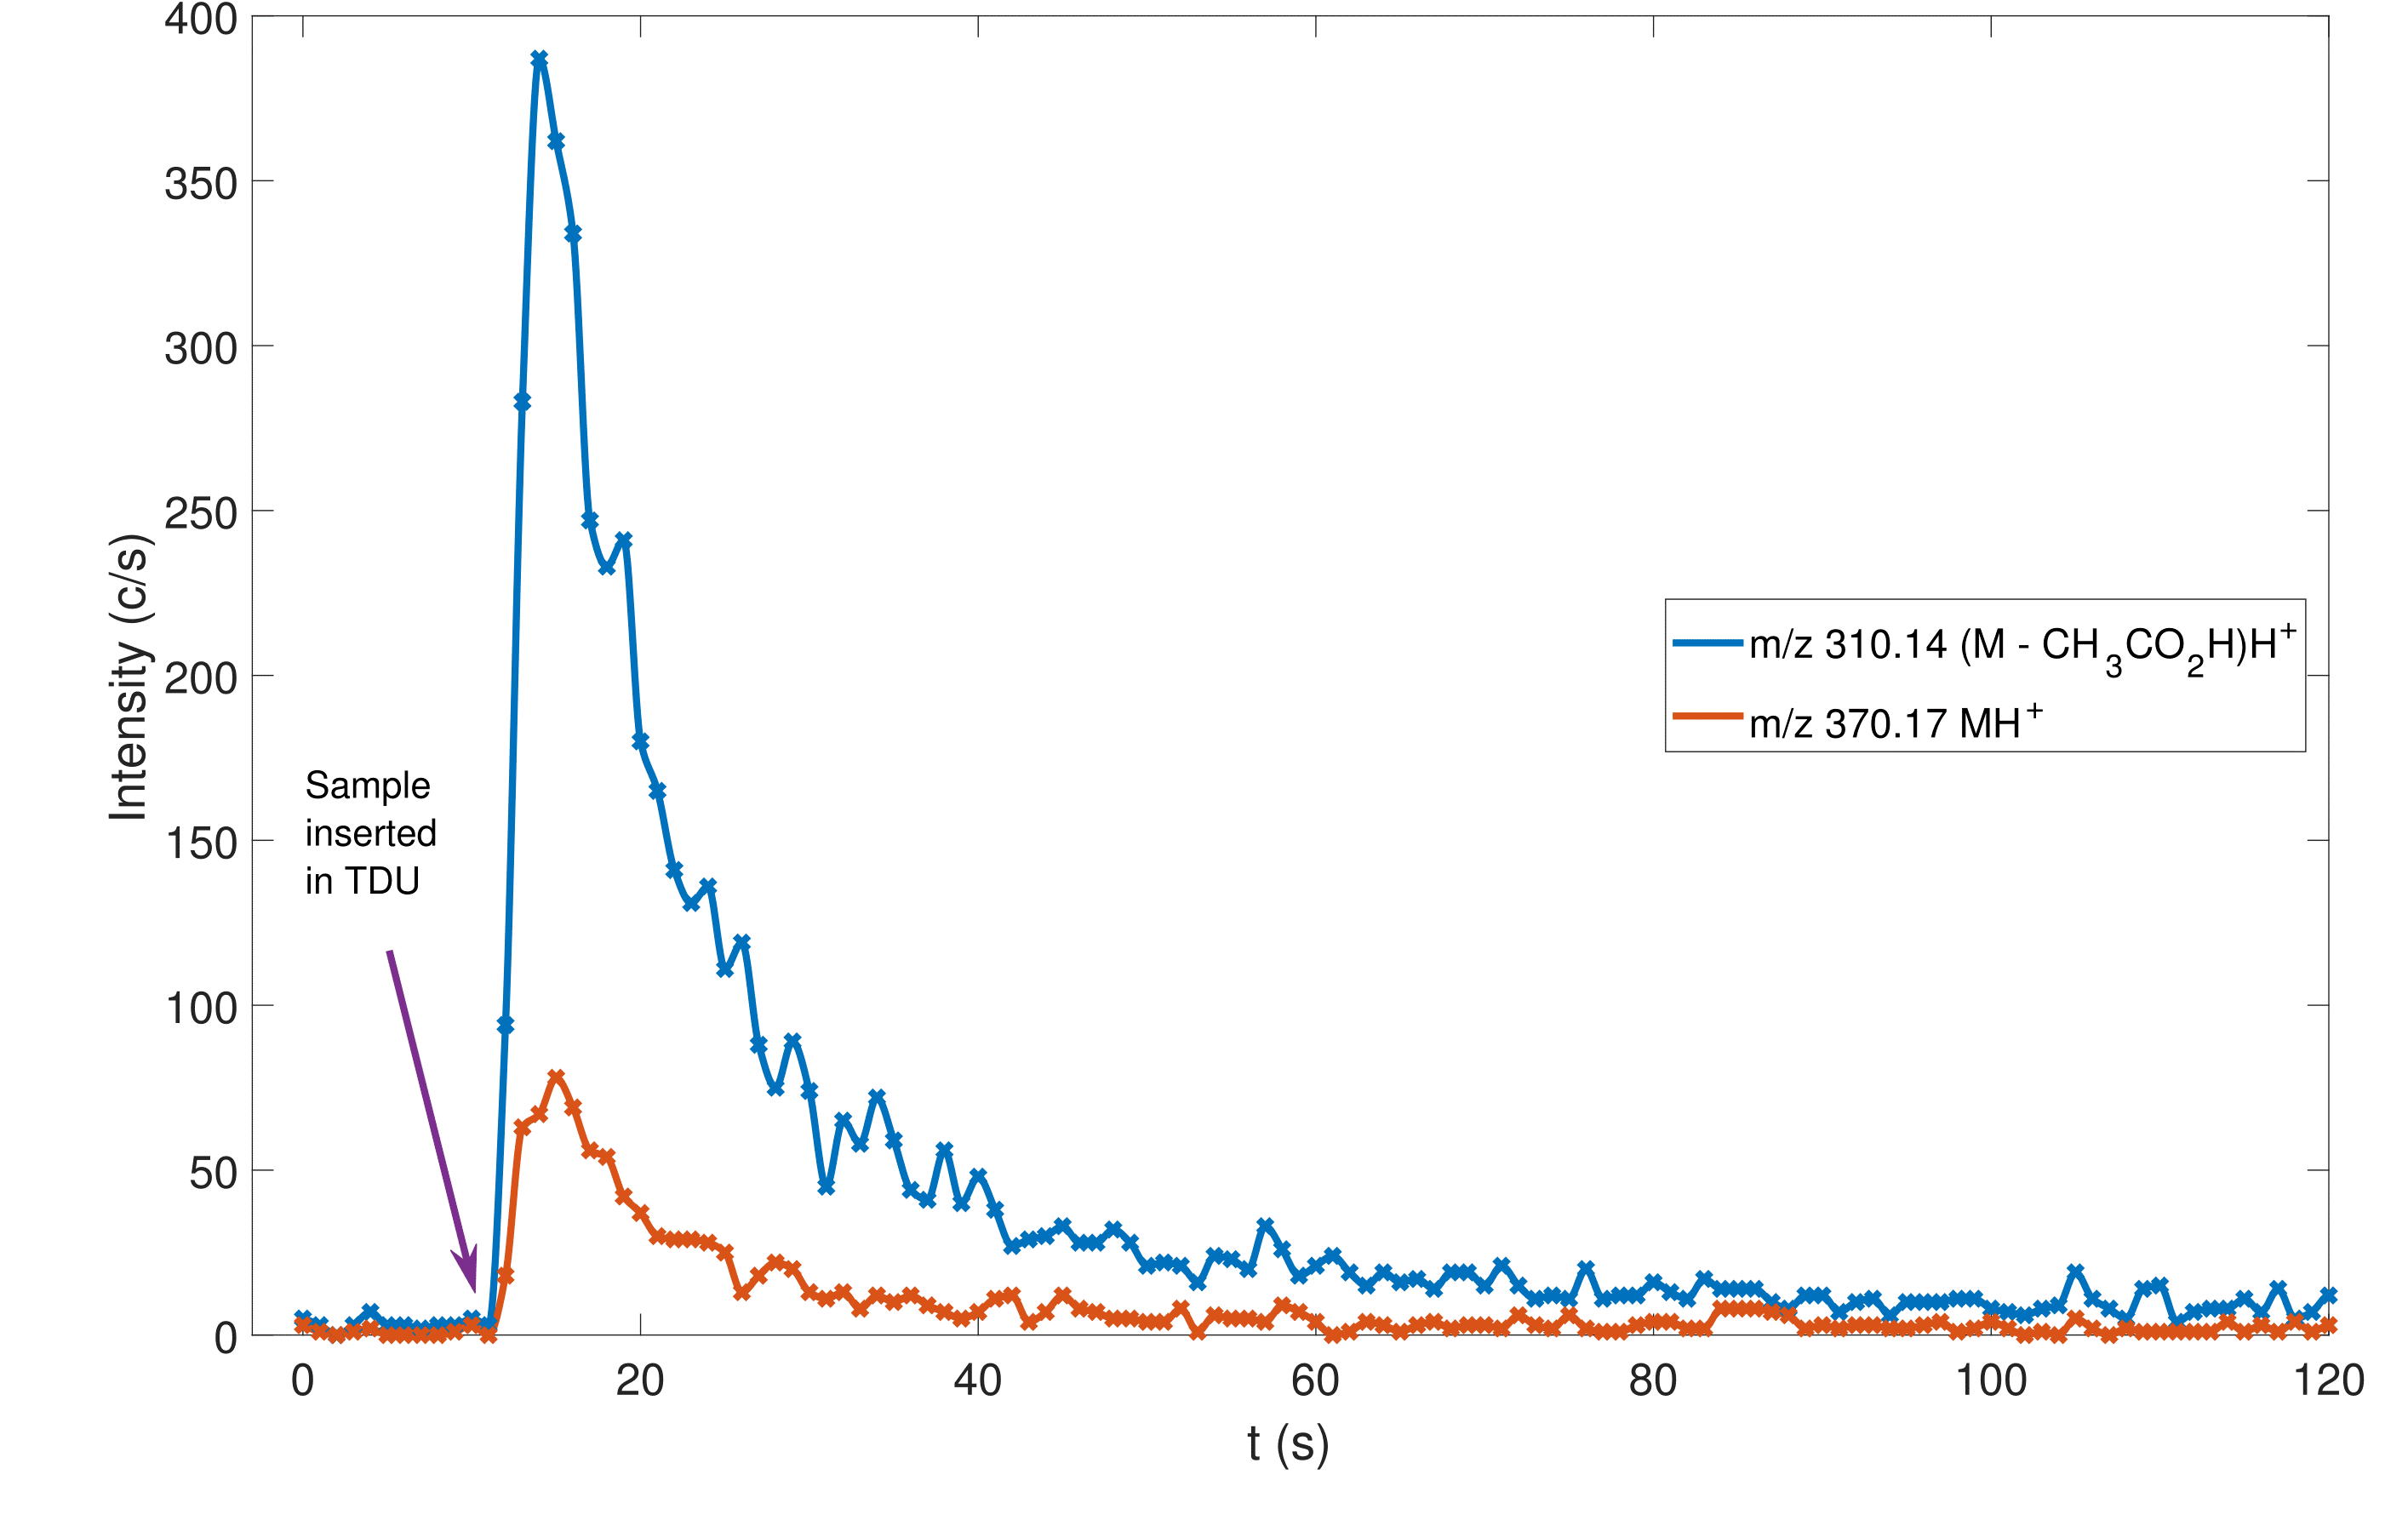
\includegraphics[width=0.7\linewidth]{pics/heroin_desorption.png}
  \caption{Time profiles of the count rates of two characteristic product ions at \textit{m/z} 310 and \textit{m/z} 370 during the thermal desorption of trace amounts of heroin at 120 Td using the TDU in PTR-MS.}\label{fig:tdu_heroin}
\end{figure}



\subsection{FastGC}\label{section:fastgc}

The fastGC (IONICON Analytik GmbH, Austria) is an add-on that aids in the product ion identification process by separating the analyte molecule from possible contaminants and impurities.

The working principle of the fastGC is the same as that of gas chromatography (\acrshort{gc}) systems, where
%
the components of a  gas mixture (mobile phase) present different retention times when flowing through a liquid or solid (stationary phase) packed inside a capillary column, which  separates them temporarily.
%
This separated mixture can be then injected into an analytical instrument for compound identification, where ion peaks occurring at the same retention time as the parent ion correspond to product ions.
%
The main differences between  GC and fastGC are that GC columns are tens of meters long, while fastGC ones are  10 meters long or less, and
%
also that the heating ramp in fastGC  is up to forty times faster than in conventional GC systems.
%
These characteristics make possible to perform a fastGC analysis in few minutes.



The fastGC was used in conjunction with a PTR-ToF 8000 (IONICON Analytik GmbH, Austria) to study the reactions of several ketones with H$_3$O$^+$ \cite{malaskova2019compendium}.
This add-on was used to ease the ion identification as the purity of the ketones was in the range 97 - 99\% and also decomposition of the sample could have occurred during storage.
%
This fastGC  is a modification of that used by \citeauthor{ruzsanyi2013multi} and \citeauthor{romano2014wine} \cite{ruzsanyi2013multi,romano2014wine}. Therefore only the differences with those will be briefly described here.
%
%The ketones were first introduced into a 0.5 ml sample loop  of passivated stainless steel.
%
The stationary phase in our system was a MXT-1 column (10 m × 0.53 mm, film thickness 0.25 µm, dimethyl polysiloxane phase, Restek, USA), which was heated from room temperature up to 240$^{\circ}$C in  2 minutes and 40 seconds.
%
Also, a 10-port passivated valve (VICI AG, Switzerland) and a three-way gas valve made from polyether ether ketone (\acrshort{peek}) replaced the four three-way valves and  needle valve in the previous design.
%
All sections of the inlet system are mounted in the oven which houses the drift tube to avoid cold spots.
%
This updated configuration allowed the sample loop to be constantly filled and the capillary column to be constantly back-flushing with the carrier gas.
%
The  carrier gas and make-up gas flows used were  8 ml/min and 20 ml/min of 6.0 N$_2$.







% this is literal from the article

%A custom-made valve block consisting of four three-way valves and a needle valve has been replaced by a 10-port passivated valve (VICI AG, Switzerland) and a three-way gas valve made from polyether ether ketone (\acrshort{peek}) was used.
%All parts of the inlet system are installed within the oven that houses the drift tube to prevent cold spots.
%This revised setup enabled constant filling of the sample loop and constant back- flushing of the capillary column with the carrier gas.
%8 ml/min and 20 ml/min of 6.0 N2 were used as carrier gas and make-up gas, respectively.


%A voltage ramp of 0.5 V/s from 10V up to 80V was applied raising the temperature of the capillary column reaching up to 240$^{\circ}$ from room temperature at a rate of up to 20$^{\circ}$C/second.































\subsection{Liquid Calibration Unit}\label{section:lcu}
The liquid calibration unit (\acrshort{lcu}, IONICON Analytik GmbH, Austria) %\citeauthor{ioniconlcu}, Austria)
is a standalone device that can be coupled to trace gas analysers for calibration purposes
where liquid standards are evaporated into a gas stream to yield known trace concentrations. % of the liquid.

%The main components of the LCU (\citeauthor{ioniconlcu}, Austria) are the nebuliser and the evaporation chamber.
The working principle of the LCU  has been explained in detail by \citeauthor{fischerlcu} \cite{fischerlcu}.
%
The  liquid sample is pumped from its container by a liquid flow controller into the nebuliser (X175, Burgener Research\textsuperscript{\textregistered}), where it mixes with the carrier gas (N$_2$ or zero air).
%
The nebulisation process creates a stream of micro-droplets that is then injected into the evaporation chamber.
%
This chamber is held at 100$^{\circ}$C to continue the process of evaporation, leading in a continuous flow of a known trace gas dilution that is then injected through a heated sampling line into the analytical instrument.

The LCU was used to study the reactions of several ketones with H$_3$O$^+$ in humid conditions \cite{malaskova2019compendium}.
This add-on was not used to calibrate the instrument but to create a steady signal of ketones samples in humid conditions. % at 100\% relative humidity at 37$^{\circ}$C.
%The one used in this study was manufactured by \citeauthor{ioniconlcu} and it has been explained in detail by \citeauthor{fischerlcu} \cite{fischerlcu}.
%
The sampling vials, kept at 30$^{\circ}$C, contained  trace quantities of  ketones  diluted in 100 ml of purified water and were  connected to the liquid inlet of the LCU. The liquid sample flow was of 35 µl/min, which with the carrier gas (N$_2$) flow of 950 ml/min gave an absolute humidity of 5\%.
%









%\chapter{%ENHANCEMENT OF SELECTIVITY IN 
%PTR-MS AND ITS APPLICATIONS IN HOMELAND SECURITY% FOR THE DETECTION OF ILLICIT DRUGS
%}
%\markboth{PTR-MS  IN HOMELAND SECURITY }{}

\chapter{Theoretical and experimental investigations of cocaine and related compounds in PTR-MS}\label{chapter:cocaine}
\markboth{Cocaine and related compounds in PTR-MS}{}
 
In this chapter a PTR-MS study of cocaine and associated compounds (e.g. cocaethylene, methyl ecgonine, ethyl ecgonine and benzoate esters) is presented, together with the proton affinity, gas-phase basicity and energetics corresponding to the structures and transition states arising from reaction of these compounds with (H$_2$O)$_n$H$_3$O$^+$ (n = 0, 1, ...), which were computed using density functional theory by Dr Peter Watts.
 
\section{Introduction}


Cocaine is one of the illicit   drugs most consumed  worldwide.
%
For instance, a one-week long study in March  for 5 years to asses the drugs found in a wastewater treatment plant in Barcelona (Spain) from \citeauthor{mastroianni2017five} found that only the use of cannabis is higher than that of cocaine in that region \cite{mastroianni2017five}.
%
According to the \textit{World Drug Report 2019} from the \textit{United Nations Office on Drugs and Crime}, the global produced and seized quantities of cocaine have increased three-fold in the period 1998-2018, with a nearly two-fold raise in the seized amount in the period 2014-2017 from 652 to 1275 metric tonnes (see \autoref{fig:coc_UN})
 \cite{united2019world}.
%
The consumption of illicit drugs involves drug trafficking from the manufacturing countries in South America to the  consumers (e.g. North America and Europe).
%
Because of this, law enforcement agencies need to  detect cocaine and similar compounds rapidly and with a high level of confidence in locations where outstanding amounts of goods are exchanged, like airports and ports. One real time analytical technique that can provide this is PTR-MS.  To be able to use this instrument in the field, we first need to determine and understand the protonation and fragmentation processes that cocaine and related compounds undergo as a function of the key operational parameter, namely the reduced electric field, which is the ratio of the electric field strength to the gas number density in the drift tube.


\begin{figure}[ht]
\centering
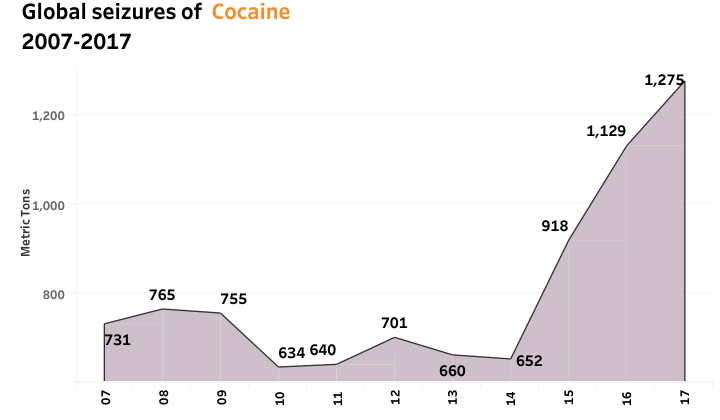
\includegraphics[width=0.8\linewidth]{pics/cocaine-chapter/UN_coc.png}
\caption{Metric tons  of worldwide seized cocaine per year in the 2007-2017 period \cite{united2019world}.}
\label{fig:coc_UN}
\end{figure}

PTR-MS has already proved to be a useful tool for the detection of drugs. 
%
E. g. 
\citeauthor{doi:10.1002/jms.2993} successfully  used PTR-MS to detect rape drug mixed with drinks  and \citeauthor{lanza2013distinguishing} proved that ion-molecule processes can be manipulated to differentiate between isomeric substances without initial pre-separation \cite{doi:10.1002/jms.2993,lanza2013distinguishing}.
%
%
The  PTR-MS studies of cocaine in the literature have  limitations. 
%
For example,  \citeauthor{Agarwal2011} only reported the product ions obtained from the analysis of several drugs at a reduced electric field of 120 Td, which is useful information at the standard conditions the PTR-MS are often used at, but at the same time this data lacks the spread in collisional energy that the  PTR-MS instruments can be operated at to improve selectivity \cite{Agarwal2011}.


%\textbf{(Explain all metabolites and if they are minor major etc, when they come from etc from the paper!!!!!!!)}

Cocaine is a schedule 2 drug. 
%
%When it is consumed, the person feels euphoria for ..... minutes....
The pharmacokinetics depends on the route of administration, with the peak of the effect occurring after 1-5 minutes being smoked or injected and after 15-20 minutes after being snorted  \cite{lange2001cardiovascular}.
%
These high effects, which are mainly euphoria and restlessness (i.e. urge to move), wash out after 5-15 minutes for smoked cocaine, 20-60 minutes for injected cocaine and 60-90 minutes for snorted cocaine.
%
%
Cardiovascular complications are the main outcome of cocaine abuse.
%
%The health issues associated to cocaine abuse
These are predominantly coronary heart disease and arrhythmias, due to the fact that cocaine causes vasoconstriction of blood vessels, which presents risks for the heart and brain.
%
Deaths related to cocaine overdose are usually attributed to respiratory failure, cardiac arrhythmias and rupture of arteries due to a large increase in arterial pressure \cite{lange2001cardiovascular,cregler1986medical}.
%
Also psychological and psychiatric (e.g. depression and paranoid psychosis), neurological, renal, pulmonary, gastrointestinal, obstetrical, and otolaryngological complications have been reported as a consequence of cocaine abuse \cite{glauser2007overview}.
%


%The short wash out period of cocaine
%addiction 
%catastrophic for familoes...


Only around 1\% of the consumed cocaine is retrieved through excretion in the few hours after intake.
%
The rest of it is converted into %water-soluble 
metabolites that can be detected in urine up to 24-36h after consuming the drug or in hair samples potentially up to several weeks later \cite{cone1991testing}. 
%
The main metabolites arising from cocaine consumption are: 
benzoylecgonine, 
ecgonine methyl ester, 
ecgonine ethyl ester, 
cocaethylene,
norcocaine,
methylecgonidine and 
hydroxycocaines.


Benzoylecgonine and %methylecgonidine (also known as ecgonine methyl ester)
ecgonine methyl ester (also known as methyl ecgonine)
are the main metabolites of cocaine, which  are formed when cocaine undergoes deesterification through hydrolysis in the liver \cite{shimomura2019cocaine}.
%
Like most cocaine metabolites, benzoylecgonine and methylecgonidine are inactive and hence do not induce any toxicity effects when present in the human body.
%
These two are the metabolites that are normally screened in urine tests, for whose analysis GC-MS is commonly used. This technique requires a derivatisation process of the samples prior the chemical analysis, which is time-consuming.
\citeauthor{ambre1988urinary}  performed methylation of benzoylecgonine to transform it back to cocaine 
while
\citeauthor{fleming2010quantitation} detected benzoylecgonine and methylecgonidine as pentafluoropropionyl derivatives
\cite{ambre1988urinary,fleming2010quantitation}.
%
On the contrary, techniques that do not require derivatisation are, for example, HPLC and that developed by  \citeauthor{hezinova2012simultaneous}  
\cite{antonilli2001analysis,hezinova2012simultaneous}.

%____________________________________________________________________

Cocaine users are often heavy drinkers of alcohol.
%
When both cocaine and ethanol are present in the bloodstream, the active metabolite cocaethylene is produced in the body, which in itself is a recreational drug with similar (i.e. euphoria and increased heart rate) but stronger effects than those of cocaine  \cite{mccance1993concurrent,pennings2002effects}. 
%
Cocaethylene is formed in the liver through the transesterification of around 15-20\% of the consumed cocaine, which occurs  3.5 times faster than deesterification to benzoylecgonine
\cite{jatlow1991cocaethylene,snozek2012cocaine,harris2003pharmacology}.
%
The toxicity effects of cocaethylene are not only stronger and longer-lasting than those of cocaine. 
The amount of cocaine found in dead bodies when alcohol was also found was lower than in cases where only cocaine was present, indicating that cocaethylene is also a deadlier substance
 \cite{lange2001cardiovascular}.
%
Furthermore, ecgonine ethyl ester (also known as ethyl ecgonine) is produced from cocaethylene through deesterification in a similar way ecgonine methyl ester is produced from cocaine.

%Ethyl ecgonine is a deesterification product of cocaethylene that is formed through hydrolysis.
%
%It is a minor metabolite of cocaine and it is only present together with cocaethylene, but it was included in this study because of its similarities to methyl ecgonine. 
 

%___________________________________________

Another active metabolite of cocaine is norcocaine.
This metabolite is found in low amounts compared to benzoylecgonine and ecgonine methyl ester, but its presence in blood increases when alcohol is consumed at the same time \cite{farre1993alcohol}.
%
It is formed through the demethylation of the pyrolidine nitrogen in cocaine and, like cocaethylene, norcocaine has been also found in hair samples from cocaine users \cite{cone1991testing}.

%_________________________________

Crack (also known as cocaine base) is the smokable form of cocaine.
%
It receives this name because of the cracking sound it makes when heated to be inhaled.
%
%
The main pyrolysis product of cocaine is methyl ecgonidine (also known as anhydroecgonine methyl ester), which is formed when crack cocaine is decomposed at high temperatures.
%
It has been found in the excretions from crack smokers and
\citeauthor{wood1996methylecgonidine} estimated  the amount of produced methyl ecgonidine to be around 5\% of the smoked cocaine \cite{anhydroecgoninemethylester,wood1996methylecgonidine}.

%___________________________________________________________________________


Hydroxycocaines form a group of lesser-known cocaine metabolites because of their low abundance relative to that of other metabolites.
%
This family consists of  different isomeric compounds whose structural difference only resides on the carbon atom of the benzene ring the hydroxy group is attached to, yielding three structures: o-, m- and p-hydroxycocaine. 
%
These metabolites have been detected using different analytical techniques  in human hair,  blood and urine   \cite{schaffer2016analysis,paul2005concentration,robandt2008complete,klette2000simultaneous,cone1991testing}.
%
%O-hydroxycocaine (also known as salicylmethylecgonine and 2'-hydroxycocaine) is speculated to be an active metabolite \cite{}




%_________________________________

Besides the mentioned metabolites, cocaine also decays to  other  compounds.
%
One of the  degradation products of cocaine is methyl benzoate, whose production is enhanced at higher humidities.
%
\citeauthor{furton2002identification} linked the reaction of canine  units to solid-phase microextraction gas chromatography  stating that dogs react more to methyl benzoate  than to cocaine itself, while \citeauthor{waggoner1997canine} also proved that the canine units react to both methyl benzoate and cocaine samples, but with inconclusive results of whether it is methyl benzoate the compound dogs are reacting to
\cite{furton2002identification,waggoner1997canine}.


%__________________________________________________________________________

A brief introduction of the main metabolites of cocaine was provided above to provide context for this chapter.
%
However, PTR-MS will hardly be used as an analytical tool for the screening of these substances because other techniques (e.g. GC-MS or HPLC) are the standard tools already established  in each field.
%
Therefore the reason some  cocaine metabolites were included in this study was to shed some light in the PTR-MS and DFT results from other compounds and, at the same time, potentially be the basis for future research involving other analytical techniques.












%It is very important to note that this is (using PTR-MS as research tool, not like analytical device). Hence, some of the metabolites analysed here lack practical applications but can shed some light in the PTR-MS and DFT results from other compounds and at the same time be the basis for future studies involving other analytical techniques.






\section{Methodology}
 
\subsection{Experimental details}\label{section:coc_expdet}
%TDU, Temperatures, pressures,
The KORE Technology Ltd PTR-ToF-MS instrument described in \autoref{chapter:ptr} was used for this experiment. 
The reactor was kept at a pressure of 1 mbar and at 150$^\circ$C throughout all the experiments, while the pressure in the hollow cathode was set at 1.1 mbar for normal measurements and 1.4 mbar for humid ones. More details of this are given in \autoref{section:coc_RI}.


\subsection{Chemicals}
All the substances used in this study were acquired from Sigma Aldrich. Some of the samples were sourced as solids diluted in organic solvents: cocaine (1 mg/mL in acetonitrile, certified reference material), methyl ecgonine (1 mg/mL in acetonitrile, certified reference material), cocaethylene (1 mg/mL in acetonitrile, certified reference material), ethyl ecgonine (1 mg/mL in acetonitrile, certified reference material), norcocaine hydrochloride (1 mg/mL in acetonitrile (as free base), certified reference material), o-hydroxycocaine (1 mg/mL in acetonitrile, certified reference material) and methyl ecgonidine (1 mg/mL in acetonitrile, certified reference material). These were further diluted using HPLC grade solvents to give a concentration of 100 µg/mL. Although cocaine is a schedule 2 drug, no license is required for research purposes given that (i) it is acquired dissolved in a solvent from which it cannot be recovered from, (ii) it is not for human or animal use, and (iii) minimal quantities (i.e. mg level or less) are used.
The benzoates (i.e. methyl, ethyl and isopropyl benzoate) and the isobutyrates (i.e. methyl and ethyl isobutyrate) esters are colourless liquids. Benzoic acid is a white crystalline powder. These liquid substances and benzoic acid were acquired with a purity of at least 99\% and were used without further purification.



\subsection{Sampling methods}%: thermal desorption unit and headspace analysis}
Cocaine is a white solid with a vapour pressure of 2.5$\times$10$^{-7}$ mbar  at 25$^\circ$C, which makes challenging to detect it without any pre-separation system \cite{cocaineVP55}.
%
%O preheating
%
%Also add boiling temperature.
%
\citeauthor{RN445} implemented a thermal desorption unit to tackle this low vapour pressure issue for explosives and \citeauthor{blenkhorn2019novel} applied it to the detection of polyaromatic hydrocarbons \cite{RN445,blenkhorn2019novel}.
The same thermal desorption unit was used for this study to desorb the diluted samples into the PTR-MS instrument.
%
%Details of this TDU have been given elsewhere \cite{RN445}.
A volume of 1-5 µL of the diluted samples was spotted onto the PTFE swab and it was inserted into the TDU after waiting 1 minute for the solvent to evaporate. The carrier gas, in this case oxygen-free nitrogen (99.998\% purity, BOC Gases, Manchester, UK), drags the analyte through the heated inlet pipe and into the drift tube, creating a desorption “pulse” of 10 - 20 seconds depending on the analyte (see \autoref{fig:tdu_heroin}).


The liquid samples and benzoic acid are more volatile and were studied by means of headspace analysis. Oxygen-free nitrogen was used as carrier gas to drag the headspace of 22 mL vials containing trace amounts (<1 mL) of the samples, which were also connected to the inlet line of the instrument. 

\subsection{Density functional theory}
DFT calculations have been undertaken to determine  proton affinities,  gas-phase basicities  and to study the energetics of the formation of the main product ions of interest. All calculations use the B3LYP functional and the 6-31+G(d,p) basis set at a temperature of 298 K.

%\newpage

\section{DFT and PTR-MS results}
%\section{Results and discussion}
The PTR-MS and DFT calculations are  presented in this section. The PTR-MS results are provided over the broadest achievable \textit{E/N} range: approximately 20 - 255 Td, which corresponds to a drift voltage interval from 35 to 410 V (i.e. the whole  voltage range that the instrument can supply). 
The main reason for the ion counts to be low at low \textit{E/N} is the low abundance of reagent ions (see \autoref{fig:RI_coc}). 
At the same time, the residence time, which is proportional to 1/(\textit{E/N}), is much higher at low \textit{E/N} and the ions spend longer in the drift tube than at high \textit{E/N}, which results in more collisions with the buffer gas and a higher chance of proton transfer from the reagent ions to analyte molecules. 
%
%As it can be seen in \autoref{fig:RI_coc} the availability of reagent ions is around five times higher in humid conditions, but so is the presence of water clusters from which the proton transfer is softer because their PA is higher than that of the water monomer (see \autoref{tb:pa}).
%



%Please note that the starting point of the data at low \textit{E/N} is not exactly the same for all the measurements. This is like that because the lower end of the data was going to be discarded but I decided to include it in the end.
%
%The reason that the drift voltage and \textit{E/N} are not exactly identical in all the plots is because there were small differences in the drift tube pressure from experiment to experiment.
%
%
%The plots are included in counts per second rather than in branching percentages because the branching percentage can hide relevant (effects?) and display misleading (behaviours?)/be misleading and do not give an idea of the total ion counts.
%

The compounds analysed in this chapter are summarised in \autoref{tab:COC_structs} and \autoref{tab:COC_structs2}, including their nominal molecular weight, vapour pressure, chemical formula and structure.
%
The vapour pressure values in these tables have been taken from the United States Environmental Protection Agency Chemistry Dashboard \cite{USAEPA}. These are experimental values except for that of methyl ecgonine, ethyl ecgonine, cocaethylene and methyl ecgonidine, which are the predicted vapour pressures.
%
 In the tables included in this chapter that provide the energetics relative to the protonation reaction or further fragmentation, the given \textit{m/z} refers to the detected ion, i.e. where the charge remains, and the neutrals H$_2$O or (H$_2$O)$_2$ have been omitted in all the cases.





\begin{table}
\centering
\caption{Nominal molecular weight, vapour pressure at 25$^\circ$C, formula and structure of cocaine, methyl ecgonine, cocaethylene, ethyl ecgonine, norcocaine, methyl ecgonidine and o-hydroxycocaine.}
\begin{tabular}{lcccc}
\textbf{Compound} &  \textbf{MW} & \textbf{VP (mbar)} & \textbf{Formula} & \textbf{Structure} \\ 
\toprule
Cocaine &   303 &2.5$\times$10$^{-7}$ &  C$_{17}$H$_{21}$NO$_4$ & \begin{minipage}[c]{0.26\linewidth}\centering 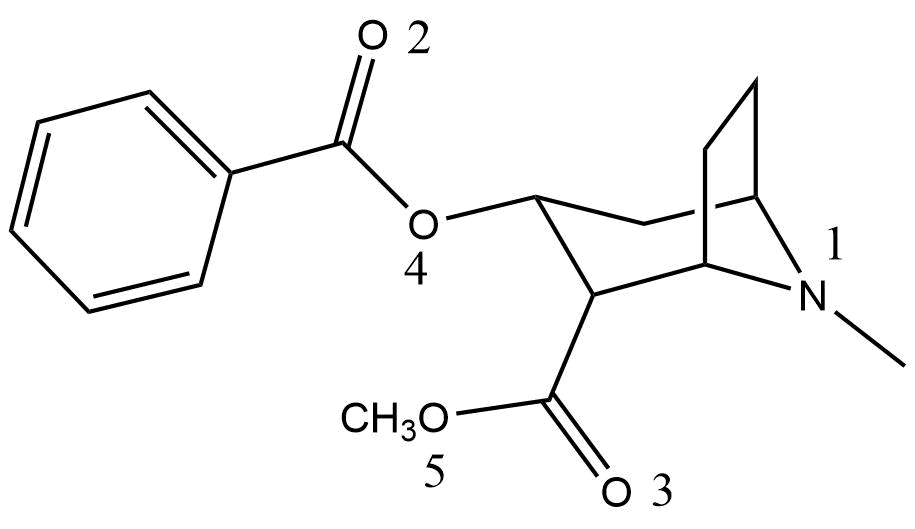
\includegraphics[width=\linewidth]{pics/cocaine-chapter/COC_struct.png}\end{minipage}\\ \midrule
Methyl ecgonine & 199 & 4.9$\times$10$^{-5}$& C$_{10}$H$_{17}$NO$_3$ & \begin{minipage}[c]{0.26\linewidth}\centering 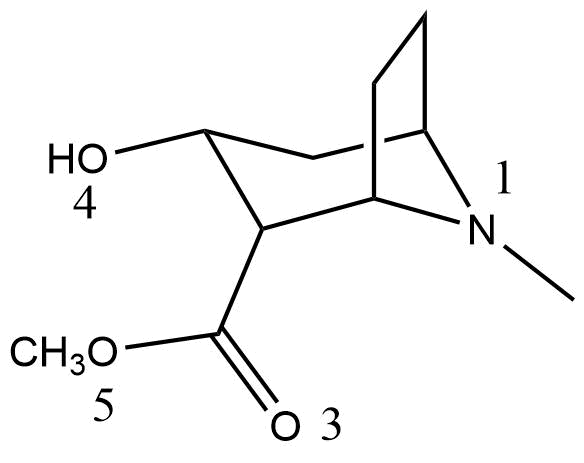
\includegraphics[width=.8\linewidth]{pics/cocaine-chapter/MeEcg_struct.png} \end{minipage} \\ \midrule
Cocaethylene & 317   &1.0$\times$10$^{-6}$ &  C$_{18}$H$_{23}$NO$_4$ & \begin{minipage}[c]{0.26\linewidth}\centering 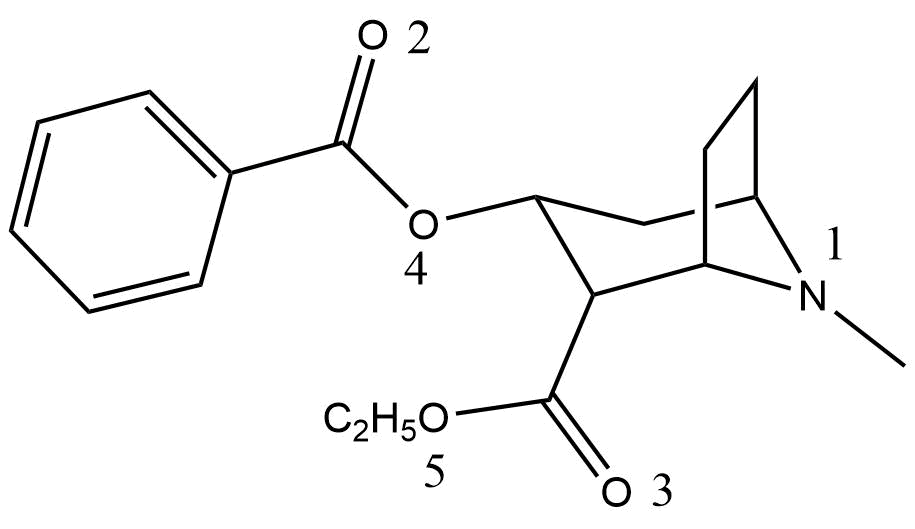
\includegraphics[width=\linewidth]{pics/cocaine-chapter/cocaet_struct.png} \end{minipage} \\ \midrule
Ethyl ecgonine & 213 & 7.8$\times$10$^{-6}$ &C$_{11}$H$_{19}$NO$_3$ & \begin{minipage}[c]{0.26\linewidth}\centering 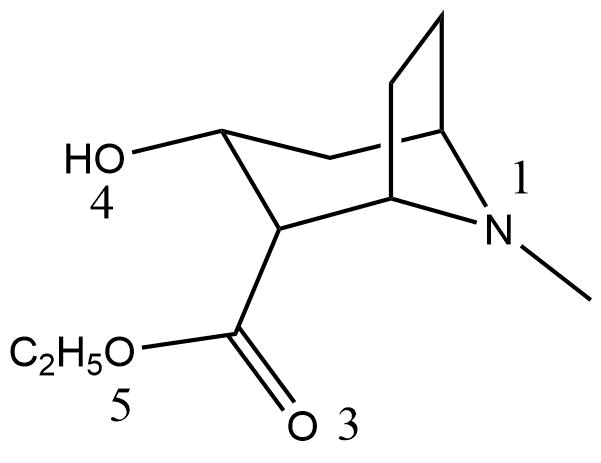
\includegraphics[width=.8\linewidth]{pics/cocaine-chapter/EtEcg_struct.png} \end{minipage} \\ \midrule
Norcocaine & 289 & - &C$_{16}$H$_{19}$NO$_4$ & \begin{minipage}[c]{0.26\linewidth}\centering 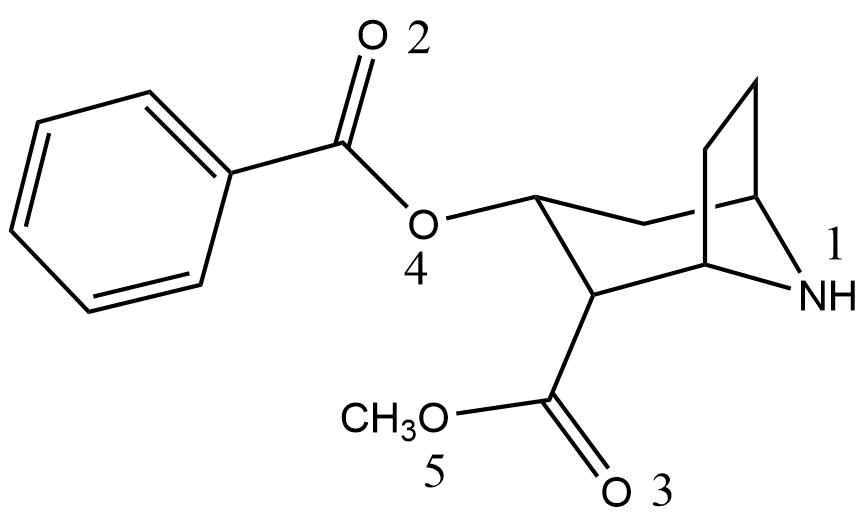
\includegraphics[width=\linewidth]{pics/cocaine-chapter/norcocaine_struct.png} \end{minipage}  \\ \midrule
Methyl ecgonidine & 181& 1.3$\times$10$^{-2}$ & C$_{10}$H$_{15}$NO$_2$ & \begin{minipage}[c]{0.26\linewidth}\centering 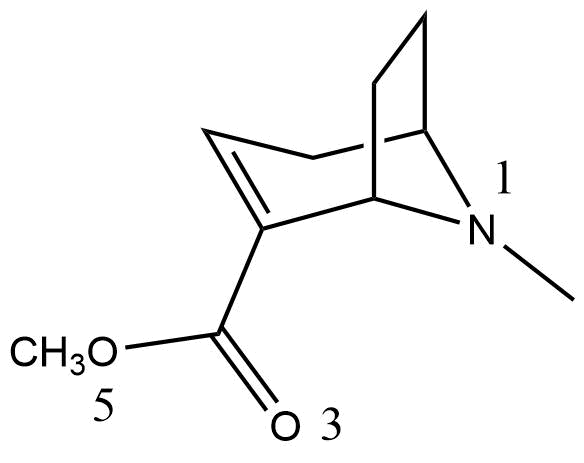
\includegraphics[width=0.8\linewidth]{pics/cocaine-chapter/ame_struct.png} \end{minipage}  \\ \midrule
o-Hydroxycocaine & 319 & - &C$_{17}$H$_{21}$NO$_5$ &  \begin{minipage}[c]{0.26\linewidth}\centering 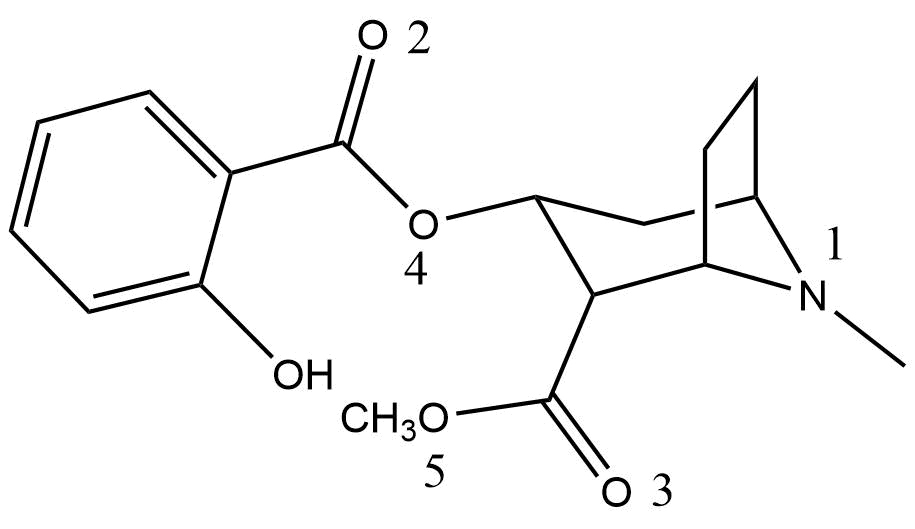
\includegraphics[width=\linewidth]{pics/cocaine-chapter/ohcocaine_struct.png} \end{minipage} \\ 
\bottomrule
\end{tabular}
\label{tab:COC_structs}
\end{table}

\begin{table}
\centering
\caption{Nominal molecular weight, vapour pressure at 25$^\circ$C, formula and structure of benzoic acid, methyl benzoate, ethyl benzoate, isopropyl benzoate, methyl isobutyrate and ethyl isobutyrate.}
\begin{tabular}{lcccc}
\textbf{Compound} &  \textbf{MW} & \textbf{VP (mbar)} & \textbf{Formula} & \textbf{Structure} \\ 
\toprule
Benzoic acid &   122 &9.3$\times$10$^{-4}$&   C$_{7}$H$_{6}$O$_2$ & \begin{minipage}[c]{0.085\linewidth}\centering 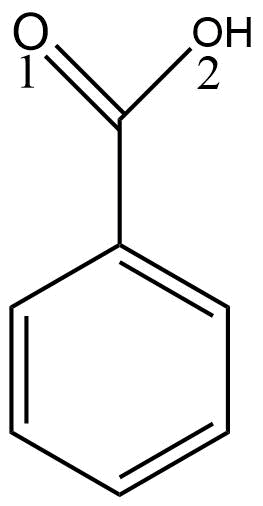
\includegraphics[width=\linewidth]{pics/cocaine-chapter/bzacid_struct.png}\end{minipage}\\ 
\midrule
Methyl benzoate &   136 &0.51&  C$_{8}$H$_{8}$O$_2$ & \begin{minipage}[c]{0.085\linewidth}\centering 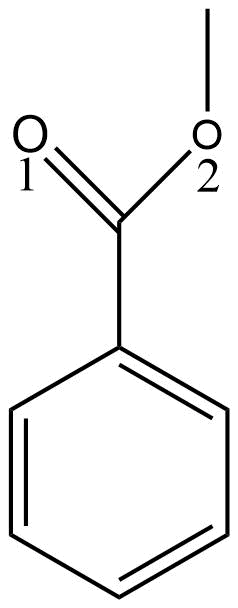
\includegraphics[width=\linewidth]{pics/cocaine-chapter/MeBz_struct.png}\end{minipage}\\ 
\midrule
Ethyl benzoate &   150 &0.36&   C$_{9}$H$_{10}$O$_2$ & \begin{minipage}[c]{0.105\linewidth}\centering 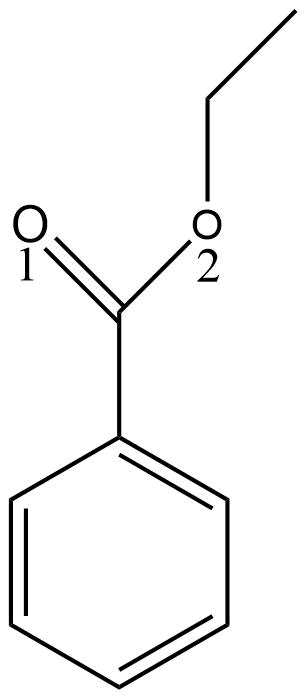
\includegraphics[width=\linewidth]{pics/cocaine-chapter/EtBz_struct.png}\end{minipage}\\ 
\midrule
Isopropyl benzoate &   164 &4.6$\times$10$^{-4}$&   C$_{10}$H$_{12}$O$_2$ & \begin{minipage}[c]{0.105\linewidth}\centering 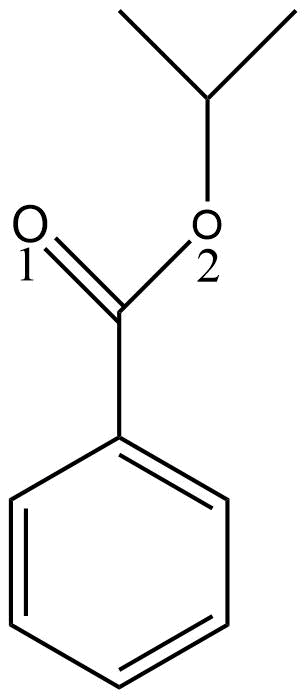
\includegraphics[width=\linewidth]{pics/cocaine-chapter/iPrBz_struct.png}\end{minipage}\\ 
\midrule
Methyl isobutyrate &   102 &65.7&   C$_{5}$H$_{10}$O$_2$ & \begin{minipage}[c]{0.13\linewidth}\centering 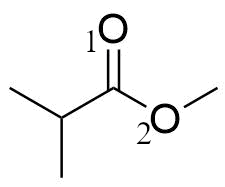
\includegraphics[width=0.8\linewidth]{pics/cocaine-chapter/MEisobuty_struct.png}\end{minipage}\\ 
\midrule
Ethyl isobutyrate &  116 &33.9&   C$_{6}$H$_{12}$O$_2$ & \begin{minipage}[c]{0.17\linewidth}\centering 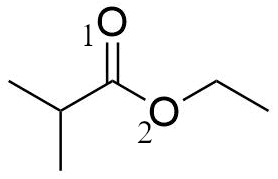
\includegraphics[width=0.8\linewidth]{pics/cocaine-chapter/ETisobuty_struct.png}\end{minipage} \\
\bottomrule
\end{tabular}
\label{tab:COC_structs2}
\end{table}



\subsection{Reagent ions}\label{section:coc_RI}
For many of the compounds discussed in this chapter, a ``normal'' and humid \textit{E/N} study was done.
%
The reagent ion signal for hydronium and the corresponding water cluster for these two sets of data are shown in \autoref{fig:RI_coc} and the PA and GB of  the water and its oligomers that yield (H$_2$O)$_n$H$_3$O$^+$ ions are given in \autoref{tb:pa_h2o}.
%
The abundance of the different water cluster species (i.e. (H$_2$O)$_n$H$_3$O$^+$) as a function of the reduced electric field that is observed in these figures are in agreement with those reported by \citeauthor{price1977new} as a function of the  reactor pressure, temperature and the \textit{E/P} ratio \cite{price1977new}.



\begin{table}[htbp]
\centering
\caption{Proton affinity and Gibbs free energy of water and its oligomers to yield the (H$_2$O)$_n$H$_3$O$^+$ (n = 0, 1, 2, 3) reagent ions.}
\label{tb:pa_h2o}
\begin{tabular}{lcc}
\toprule
\textbf{Structure} &\textbf{PA (kJ/mol)} &\textbf{GB (kJ/mol)}\\ \toprule
H$_3$O$^+$              &684  &653       \\
(H$_2$O)H$_3$O$^+$      &842  &777       \\
(H$_2$O)$_2$H$_3$O$^+$  &937  &841       \\
(H$_2$O)$_3$H$_3$O$^+$  &1013  &886       \\
\bottomrule
\end{tabular}
\end{table}

\begin{figure}[htbp]
\centering
\sidesubfloat[]{\includegraphics[width=0.8\linewidth]{pics/cocaine-chapter/RI.png}\label{fig:RI_coc_dry}}\\
\sidesubfloat[]{\includegraphics[width=0.8\linewidth]{pics/cocaine-chapter/humid/ri.png}\label{fig:RI_coc_humid}}
\caption{Reagent ion intensities in counts per second as a function of the drift voltage and the reduced electric field in (a) normal and (b) humid conditions.}
\label{fig:RI_coc}
\end{figure}

A higher humidity in the drift tube can be achieved by increasing the humidity in the buffer gas, like \citeauthor{malaskova2019compendium} did \cite{malaskova2019compendium}. However, the measurements at higher humidity were unintended in my case, as the standard parameters setting (i.e. drift tube at 1 mbar and hollow cathode at 1.3 - 1.4 mbar)  yield such amount of water cluster ions that H$_3$O$^+$ is only more abundant than  (H$_2$O)H$_3$O$^+$ at reduced electric field values of 150 Td or more (\autoref{fig:RI_coc}b), which is occurring because the (H$_2$O)$_n$H$_3$O$^+$ ions don not break up prior their injection to the drift tube. This was found after doing a whole set of experiments in these humid conditions.
%
 Nevertheless, with the proton transfer from (H$_2$O)H$_3$O$^+$ being softer than that from H$_3$O$^+$, it is also necessary to acquire data in the driest conditions that the instrument could achieve to compare that data with the humid set. 
 %
The main consequence of a high abundance of water cluster ions at low \textit{E/N} is that it gets more complicated to ascertain whether the formation of a product ion at high \textit{E/N} is due to the higher collisional energy supplied by the electric field or is a consequence of the remaining energy after a harder proton transfer as the proton donating species is different than that at low \textit{E/N}.

The hollow cathode pressure can be reduced to minimise the clustering of reagent ions.
  However, there are two limitations when reducing the hollow cathode pressure: (i) lower pressure difference between cathode and drift tube increase the back-streaming of buffer gas  into the hollow cathode, generating undesirable reagent ions, and also (ii) at lower cathode pressures the  power supply unit struggles to maintain the glow (i.e. the glow discharge indicator is flickering). 
%
A compromise was found at a hollow cathode pressure of 1.1 mbar and this drier configuration, whose reagent ion signal is shown in \autoref{fig:RI_coc}a, is referred to as ``normal'' conditions in this chapter.
%

The total reagent ion signal for each of the plots in \autoref{fig:RI_coc} present a maximum  at different values of the reduced electric field. This is correlated by the product ion plots provided in this chapter, which are given in raw counts per second to avoid the possible misleading effects created by normalising by the reagent ion signal or by calculating the branching percentages.
%
However, the raw cps do not give a quantitative measure on the abundance of ions  either, as the transmission of the ions along the different stages of the instrument depends on both the \textit{E/N} and the \textit{m/z} , but those are best quantity to use when comparing the findings from different instruments.



 
\subsection{Cocaine}
The structure of cocaine is given in \autoref{tab:COC_structs}. The main protonation sites are the pyrolidine nitrogen N1, the benzoyl oxygen O2, the carbonyl oxygen O3, and the ester oxygen atoms O4 and O5.
%
DFT calculations show that the most basic site is N1 and the most stable structure of the protonated cocaine molecule is with the proton on N1 hydrogen bonded to O3. This structure is designated cocaine1H$^+$.
%
Likewise, when the proton is on O2 or O3 the structure is named cocaine2H$^+$ or cocaine3H$^+$.
%
Direct protonation of the ester sites O4 and O5 is possible.
%
The proton was found to be able to move between the studied basic sites and hence it will reside in the most basic site (N1).
In other words, MH$^+$ will predominantly be cocaine1H$^+$.
%
The displacement of the proton  from N1 to other sites  will result in fragmentation.
%
The PA and GB for the two most stable protonation sites of cocaine, N1 and O2, are given in \autoref{tb:co1} and these indicate that cocaine can be protonated from (H$_2$O)$_n$H$_3$O$^+$ up to n = 3.
Proton transfer from (H$_2$O)$_3$H$_3$O$^+$ would be actually thermoneutral as PA((H$_2$O)$_4$) = 1013 kJ mol$^{-1}$. 

\begin{table}[htbp]
\centering
\caption{Proton affinity and Gibbs free energy of the two most stable protonation sites of cocaine to yield the structures cocaine1H$^+$ and cocaine2H$^+$.}
\label{tb:co1}
\begin{tabular}{lcc}
\toprule
\textbf{Structure} &\textbf{PA (kJ/mol)} &\textbf{GB (kJ/mol)}\\ \toprule
Cocaine1H$^+$  & 1013 &   980    \\
Cocaine2H$^+$  & 933 &   895    \\
\bottomrule
\end{tabular}
\end{table}




The product ion intensities in cps for the reaction of (H$_2$O)$_n$H$_3$O$^+$ (n = 0, 1, 2, 3)  with cocaine are plotted in \autoref{fig:cocaineEN}.
%
These agree with the product ions reported in the literature \cite{Agarwal2011,wang1998collision}.
%
The dominant ion in both the normal and humid measurements is the protonated parent molecule MH$^+$ (i.e. (C$_{17}$H$_{21}$NO$_4$)H$^+$) from non-dissociative proton transfer. 
%
There are other product ions observed with less abundance.
%
The ion at \textit{m/z} 182 (i.e. C$_{10}$H$_{16}$NO$_2^+$) is a carbocation resulting from the loss of benzoic acid from MH$^+$, while the one at \textit{m/z} 272 (i.e. C$_{16}$H$_{18}$NO$_3^+$) is an acyl following the loss of methanol (MeOH) from  MH$^+$.
%
At high \textit{E/N}, C$_{5}$H$_{8}$N$^+$ is found at \textit{m/z} 82.
%
In humid conditions two other ions are also observed: benzoyl$^+$ at \textit{m/z} 105 and protonated benzoic acid at \textit{m/z} 123.
%



 
\begin{figure}[htbp]
\centering
\sidesubfloat[]{\includegraphics[width=0.8\linewidth]{pics/cocaine-chapter/COC-CPS.png}}\\
\sidesubfloat[]{\includegraphics[width=0.8\linewidth]{pics/cocaine-chapter/humid/cocaine-cps.png}}
\caption{Product ion signal intensities in counts per second of the product ions resulting from reactions of  H$_3$O$^+$.(H$_2$O)$_n$ (n = 0, 1, 2, 3) with cocaine as a function of the drift voltage and the reduced electric field in (a) normal and (b) humid conditions.}
\label{fig:cocaineEN}
\end{figure}

The energetics associated to the formation of the studied product ions are given in \autoref{tb:co2}. 
%
These are only compared to H$_3$O$^+$ and (H$_2$O)H$_3$O$^+$ because these are the most relevant reagent ions: they are the most abundant in the 100 - 200 Td range and also proton transfer from (H$_2$O)$_2$H$_3$O$^+$ or (H$_2$O)$_3$H$_3$O$^+$ would be similar to that from (H$_2$O)H$_3$O$^+$.
%
Even with all the fragmentation pathways being thermodynamically allowed, it is surprising that MH$^+$ is the dominant ion for all the \textit{E/N} range.
%
One could think that in the humid results most of the MH$^+$ ion comes from the reaction with the water clusters (i.e. (H$_2$O)H$_3$O$^+$ and (H$_2$O)$_2$H$_3$O$^+$), but as similar proportions of product ions are observed in the normal case, this cannot be the reason.
%
It is more likely that the proton stays in the the most basic site (i.e. N1) and its transfer to other sites, which is thermodynamically allowed and needed for fragmentation to occur, does not occur fast.
%
%
%In the next paragraphs the formation process of the main product ions is discussed.


The formation of the ion at \textit{m/z} 272 is the result of the loss of MeOH in the methyl ester moiety of the protonated cocaine molecule.
%
This happen through a barrierless dissociation when the proton is in O5. 
%
The migration from the protonation site to O5 occurs through a transition state.
%
Two transition states were found, named TS2 and TS2A.
%
TS2 refers to the transfer of the proton from the more basic carbonyl oxygen O3 to the less basic ester oxygen O5 followed by the split up of the C--O5 bond.
%
TS2A is similar to TS2 with the proton migrating from the benzoyl oxygen O2 instead. %to the ester oxygen O5.
%
TS2 is marginally exergonic (i.e. -9 kJ mol$^{-1}$ for the reaction with H$_3$O$^+$) while TS2A has much lower energy requirements (i.e. -111 kJ mol$^{-1}$ for the reaction with H$_3$O$^+$).
%
Furthermore, the abundance of the ion at \textit{m/z} 272 is comparable to other fragment ions, which hints that the formation of this ion is carried out through the transition state TS2A.


%    Normally loss of MeOH from a methyl ester is relatively straightforward. The transition state is the migration of the proton from the more basic carbonyl oxygen (O3) to the less basic ester oxygen (O5) with the concomitant breaking of the C – O5 bond and barrierless dissociation of MeOH. This transition state will be designated TS2. However, a similar transition state involving the migration of a proton from the benzoyl oxygen O2 to O5 has been found and is designated TS2A. This is considerably lower in energy than TS2. Whilst TS2 is slightly exergonic and is thus an accessible pathway the similarity in in yield to the other fragmentation pathways suggests that the fragmentation involving TS2A is operative. 
    %
\begin{table}[htbp]
\centering
\caption{Energetics of the reaction of cocaine with (H$_2$O)$_n$H$_3$O$^+$ (n = 0, 1) yielding the respective structure or transition state. $\Delta$H$_{298}$ and $\Delta$G$_{298}$ are relative to cocaine and H$_3$O$^+$ and, in brackets, to cocaine and (H$_2$O)H$_3$O$^+$.}
\label{tb:co2}
\begin{tabular}{lccc}
\toprule
\textbf{Structure or transition state}	&\textbf{\textit{m/z} } &\textbf{$\Delta$H$_{298}$} &\textbf{$\Delta$G$_{298}$}\\
& &	\textbf{(kJ/mol)} &\textbf{(kJ/mol)} \\  \toprule
Cocaine1H$^+$  				&	304	& -328 (-170)  & -326 (-202)   \\ \midrule
(CocaineH$^+$ - MeOH) + MeOH   			&	272	& -138 (+20)	&-186 (-62)   \\ \midrule
(CocaineH - benzoic acid)$^+$ + benzoic acid &	182 & -272 (-114)  & -336 (-212)  \\ \midrule
(CocaineH - benzoyl) + benzoyl$^+$    	&	105	& -54 (+104)  & -104 (+20)  \\ \midrule
(Cocaine - benzoic acid) + benzoic acidH$^+$& 123	& -88 (+70)  & -144  (-20) \\ \midrule
MeOH loss: TS2 for H migration O3 to O5& & -8 (+150)  & -9 (+115)  \\ \midrule
MeOH loss: TS2A for H migration O2 to O5& & -119 (+39)  & -111  (+13) \\ 
\bottomrule
\end{tabular}
\end{table}


Possible structures for the C$_5$H$_8$N$^+$ product ion at \textit{m/z} 82 are provided in \autoref{fig:coc_82}. 
%
The nitrogen atom N1 is the most basic site of the cocaine molecule and hence the first structure was thought to be the correct one.
%
However, experiments from \citeauthor{wang1998collision} using deuterated precursor ions in a triple quadruple system also yield the product ion at \textit{m/z} 82, which proves that the deuterium (or proton in our case) is not part of this ion and therefore the right structure must be the second or the third of those in \autoref{fig:coc_82}, with the third structure being 16 kJ mol$^{-1}$ more stable than the second one \cite{wang1998collision}.
%
Furthermore, \citeauthor{wang1998collision} reported this ion in higher abundance than it was found in PTR-MS, and they also found the ion at \textit{m/z} 182 to be the dominant ion, rather than MH$^+$ as it is observed in PTR-MS. These differences can be explained in terms of the collisional energy. The range of energies used by \citeauthor{wang1998collision} was in the range 17 - 23 eV, while in PTR-MS the collisional energies are calculated to be ca. 1 eV and below (see \autoref{fig:KE}).
%
C$_5$H$_8$N$^+$ is also found in methyl ecgonine, cocaethylene and ethyl ecgonine but its formation will not be analysed for now because it is only found at a low abundance at high reduced electric fields and it is a product of field-activated collision-induced dissociation.




%The fragment ion with \textit{m/z} 82 was initially thought to have the first structure in \autoref{fig:coc_82} but experiments using D$_2$O in a Triple Quad by \citeauthor{wang1998collision} showed no inclusion of deuterium in the ion which must therefore have one of the other two structures, the final structure being marginally more stable by 16 kJ mol$^{-1}$ \cite{wang1998collision}. They also observed it in larger quantities than in the present work as did \citeauthor{clauwaert1998narrow}  \cite{clauwaert1998narrow}. It is also observed with MeEcg and other analogues of Cocaine but in such small amounts and high \textit{E/N} its formation will not be pursued further at present. It is interesting that whilst all fragmentation routes are energetically favourable (see later discussion for loss of Benzoic acid from protonated Benzoate esters) little fragmentation is observed. This could be ascribed to very little H$_3$O$^+$ being present and the dominance of MH$^+$ being due to reaction of Cocaine with \textit{m/z} 37 and \textit{m/z} 55. But since similar patterns of behaviour are observed under both wet and dry conditions whilst the mass spec of the reagent ions are very different for the two conditions (see reagent ions) this is most unlikely. A more plausible explanation is that the proton is sequestered on N1 and its migration to the fragmentation sites whilst thermodynamically feasible is very slow. 


\begin{figure}[htbp]
\centering
\includegraphics[width=0.6\linewidth]{pics/cocaine-chapter/mz82.png}
\caption{Possible structures of the fragment ion at \textit{m/z} 82 from the reaction of cocaine with (H$_2$O)$_n$H$_3$O$^+$. }
\label{fig:coc_82}
\end{figure}


The formation of C$_{10}$H$_{16}$NO$_2^+$ at \textit{m/z} 182 requires the elimination of benzoic acid from the protonated parent molecule.
%
This needs the proton to be on O2 or O4 during the transition state, after which the benzoic acid is removed (i.e. the C--O4 bond breaks), yielding protonated methyl ecgonidine (see \autoref{fig:coc_182}).
%
However, the fact that the transition state was not found and that two other ions coming from the benzoate moiety (i.e. \textit{m/z} 105 and \textit{m/z} 123) were seen only in the humid conditions drove this research to the examination of a cocaine homologue, methyl ecgonine, and a series of benzoate esters.

%    In order to eliminate Benzoic acid a proton will have to be present on either O2 or O4 during the transition state. Unfortunately, attempts to find a transition state were unsuccessful with the proton migrating to O3.  Irrespective of whether the proton is on O2 or O4 when the benzoic acid departs the resulting carbocation will have the structure shown in  \autoref{fig:coc_182}, which is a protonated methyl ecgonidine.
%
%Because of the unsuccessful search for a TS for the loss of benzoic acid to give \textit{m/z} 182 and the observation of two other ions arising from the benzoate moiety viz. \textit{m/z} 123 and \textit{m/z} 105 under wet conditions it was thought useful to examine a series of benzoate esters and related compounds.% before investigating an abbreviated homologue of cocaine, benzoyl ecgonine (BzEcg).
% Before that is was considered interesting to investigate another abbreviated homologue of cocaine, methyl ecgonine (MeEcg).
 
%At present we have no explanation as to why \textit{m/z} 105 and \textit{m/z} 123 are only seen under wet conditions.



%\begin{figure}[htbp]
%\centering
%\includegraphics[width=0.4\linewidth]{pics/cocaine-chapter/COC_struct.png}
%\caption{Structure  of cocaine, including the numbering of the main protonation sites.}
%\label{fig:cocaine_struct}
%\end{figure}




\begin{figure}[htbp]
\centering
\includegraphics[width=0.25\linewidth]{pics/cocaine-chapter/coc_182.png}
\caption{Structure of the fragment ion at \textit{m/z} 182 from the reaction of cocaine with (H$_2$O)$_n$H$_3$O$^+$.}
\label{fig:coc_182}
\end{figure}



%\begin{figure}[htbp]
%\centering
%\scalebox{0.5}{
%\begin{tikzpicture}
%\chemfig{[:180]**6(------)-[::210](=[::60]O^2)-[::-60]O^4>[::75](?[a])-[::30]-[::-60,1.4](<:[::60]H)(-[::-60]N^1?[b,{-}]-[::15])-[::90,1.1]-[::135,0.8]-[::45,1.1](?[b])(<[::0]H)-[::-60]?[a](<[::45](=[::60]O^3)-[::-60]O^5-[::60])}
%%\chemfig{[:180]**6(------)-[::210](=[::60]O)-[::-60]O>[::75](?[a])-[::30]-[::-60,1.4](<:[::60]H)(-[::120]N?[b,{-}]-[::-15])-[::-30,1.1]-[::-90,0.8]-[::-90,1.1](?[b])(<[::105]H)-[::60]?[a](<[::45](=[::60]O)-[::-60]O-[::60])} %previous version with the N in opposite way
%\end{tikzpicture}
%}\label{fig:coc}
%\caption{Cocaine}
%\end{figure}



 
 

\subsection{Methyl ecgonine}
%Methyl ecgonine (MeEcg, C$_{10}$H$_{17}$NO$_3$) is the .........From deesterification, hydrolysis in the liver
%It is used as biomarker for crack (smoked cocaine) consumption. 

The protonation sites for methyl ecgonine (MeEcg) are numbered in the same way as those for cocaine (see structure in \autoref{tab:COC_structs}). 
%
The PA and GB of the protonation sites that give the two most stable structures of protonated methyl ecgonine are given in \autoref{tb:me1}.
%
MeEcg can undergo proton transfer from (H$_2$O)$_n$H$_3$O$^+$ for n = 0, 1 and 2, as PA((H$_2$O)$_3$) = 937 kJ mol$^{-1}$.
%
The structure MeEcg1H$^+$ is with the proton on the pyrolidine nitrogen (N1) hydrogen bonded to O3. 
%
MeEcg3H$^+$ is with the proton hydrogen between and hydrogen bonded to O3 and O4.
%
Similar to cocaine, the proton can move between the protonation sites although it will be mainly  on N1. 
%


    %As with cocaine, inspection of the various protonated structures shows that the proton is mobile and has no difficulty in moving between the various basic sites although as with Cocaine it will be primarily sequestered on N1. The energetics for the two most stable structures are given in \autoref{tb:me1}.
%
    %As with cocaine when the proton is on the pyrolidine nitrogen N1 it is hydrogen bonded to O3.  In MeEcg3H$^+$ the proton is hydrogen bonded between O4 and O3. The transition state for the loss of MeOH is migration of the proton from O3 to O5 followed by the barrierless dissociation of MeOH. The energetics are similar to those found for TS2 in cocaine. However direct protonation of O5 may occur. 

\begin{table}[htbp]
\centering
\caption{Proton affinity and Gibbs free energy of the two most stable protonation sites of methyl ecgonine that yield the structures MeEcg1H$^+$ and MeEcg3H$^+$.}
\label{tb:me1}
\begin{tabular}{lcc}
\toprule
\textbf{Structure} &\textbf{PA (kJ/mol)} &\textbf{GB (kJ/mol)}\\ \toprule
MeEcg1H$^+$  & 996 &   965    \\
MeEcg3H$^+$  & 906 &   873    \\
\bottomrule
\end{tabular}
\end{table}

\autoref{fig:MeEcgEN} shows the product ion intensities  for the reaction of  (H$_2$O)$_n$H$_3$O$^+$ (n = 0, 1, 2) with  methyl ecgonine as a function of the drift voltage and reduced electric field.
%
The difference in ion intensities between the normal and humid case can be explained in terms of the reagent ion intensities for each case (see \autoref{fig:RI_coc}).
%
The observed product ions follow similar fragmentation pathways as those found with cocaine.
%
The dominant ion in both the normal and humid case is MH$^+$.
%
Other found product ions are C$_{9}$H$_{14}$NO$_2^+$ at \textit{m/z} 168 or C$_{10}$H$_{16}$NO$_2^+$ at \textit{m/z} 182, resulting from the loss of MeOH or H$_2$O from the protonated parent molecule in each case.
%
Traces of C$_5$H$_8$N$^+$ at \textit{m/z} 82 are also found at high \textit{E/N} (>140 Td) but, as mentioned in the cocaine section, this will not be further investigated.

\begin{figure}[htbp]
\centering
\sidesubfloat[]{\includegraphics[width=0.8\linewidth]{pics/cocaine-chapter/MeEcg-cps.png}}\\
\sidesubfloat[]{\includegraphics[width=0.8\linewidth]{pics/cocaine-chapter/humid/MeEcg-cps.png}}
\caption{Product ion signal intensities in counts per second of the product ions resulting from reactions of H$_3$O$^+$.(H$_2$O)$_n$ (n = 0, 1, 2) with methyl ecgonine as a function of the drift voltage and the reduced electric field in (a) normal and (b) humid conditions.}
\label{fig:MeEcgEN}
\end{figure}



\autoref{tb:me2} gives the energetics of the main structures and transition states compared to those of MeEcg and H$_3$O$^+$ or (H$_2$O)H$_3$O$^+$.
%
All the structures are exergonic with H$_3$O$^+$, with the energetics for the transition state for the loss of MeOH, TS, being  similar to the transition state TS2 for cocaine.
%
This transition state consists on the barrierless dissociation of MeOH after the proton has migrated from from O3 to O5 to yield C$_9$H$_{14}$NO$_2^+$ at \textit{m/z} 168. However, direct protonation of O5 can also take place. 
%
The formation of C$_{10}$H$_{16}$NO$_2^+$ at \textit{m/z} 182  needs the proton to be on O4.
%
Then the barrierless loss of H$_2$O takes place, with further rearrangements and bond breaking to yield the structure in \autoref{fig:MeEcg_fragment}.

\begin{table}[htbp]
\centering
\caption{Energetics relative to methyl ecgonine and H$_3$O$^+$ and, in brackets, to methyl ecgonine and (H$_2$O)H$_3$O$^+$. }
\label{tb:me2}
\begin{tabular}{lccc}
\toprule
\textbf{Structure or transition state}	&\textbf{\textit{m/z} } &\textbf{$\Delta$H$_{298}$} &\textbf{$\Delta$G$_{298}$}\\
& &	\textbf{(kJ/mol)} &\textbf{(kJ/mol)} \\  \toprule
MeEcg1H$^+$   				&	200	& -312 (-154)  & -312 (-188) \\ \midrule
(MeEcgH - MeOH)$^+$ + MeOH	&	168	& -118 (+40)  & -171 (-47)   \\ \midrule
TS for loss of MeOH			&		& +4 (+162)  	& 0 (+124)   		\\ \midrule
(MeEcgH - H$_2$O)$^+$ + H$_2$O	&	182	& -62 (+96)  & -120 (+4)   \\ 
\bottomrule
\end{tabular}
\end{table}


\begin{figure}[htbp]
\centering
\includegraphics[width=0.3\linewidth]{pics/cocaine-chapter/meecg_frag.png}
\caption{Rearrangement of the product ion at \textit{m/z} 182 from protonated methyl ecgonine.}
\label{fig:MeEcg_fragment}
\end{figure}










%\begin{figure}[htbp]
%\centering
%\includegraphics[width=0.3\linewidth]{pics/cocaine-chapter/MeEcg_struct.png}
%\caption{Structure  of methyl ecgonine, including the numbering of the main protonation sites.}
%\label{fig:MeEcg_struct}
%\end{figure}





%\begin{figure}[htbp]
%\centering
%\scalebox{0.5}{
%\begin{tikzpicture}
%\chemfig{[:-30]O^4(-[::180]H)>[::60](?[a])-[::45]-[::-60,1.4](<:[::60]H)(-[::-60]N^1?[b,{-}]-[::15])-[::90,1.1]-[::135,0.8]-[::45,1.1](?[b])(<[::0]H)-[::-60]?[a](<[::45](=[::60]O^3)-[::-60]O^5-[::60])}
%\end{tikzpicture}}
%\caption{Methyl ecgonine}\label{fig:me}
%end{figure}






\subsection{Benzoate esters and benzoic acid}
Benzoate esters are chemical substances with a benzene ring bonded to the carbon atom of a carboxylate ester. 
%
The benzoate moiety in cocaine has the structure of isopropyl benzoate.
%


Protonated methyl ecgonidine at \textit{m/z} 182 is a carbocation resulting from the loss of benzoic acid from the protonated cocaine molecule.
%
The proton needs to be on O2 or O4 for this fragmentation pathway to take place but a transition state yielding such configuration was not found as the proton went to O3 instead. %
For this reason benzoic acid (BzAcid) and some benzoate esters, namely ethyl benzoate (EtBz), methyl benzoate (MeBz) and isopropyl benzoate (iPrBz)  were included in the study.
%
Benzoic anhydride was also tested but with benzoic acid being a decomposition product of benzoic anhydride with lower vapour pressure, the results could be misleading and hence this compound was finally discarded.

%(A brief investigation of benzoic anhydride was attempted but the relative vapour pressures of benzoic acid and benzoic acid are such that the former dominated the spectrum and the attempt was discontinued.) 


%But we haven’t found it yet!!!!!!!!!!!!!!!

 
 \autoref{tb:bz1} shows the proton affinity and Gibbs free energy of the protonation sites that yield the two most stable structures of protonated benzoic acid and methyl, ethyl and isopropyl benzoate.
 %
 The suffix 1H$^+$ is used here to name protonated molecules with the proton on O1 (i.e. the carbonyl oxygen) while  2H$^+$ refers to the proton is in O2 (i.e. the alkoxy oxygen).
 %
 These protonation sites are indicated in \autoref{tab:COC_structs2}. 
%

 
 
 
%\begin{figure}[htbp]
%\centering
%\includegraphics[width=0.6\linewidth]{pics/cocaine-chapter/benzoates_struct.png}
%\caption{Structure  of (left) methyl benzoate, (centre) ethyl benzoate and (right) isopropyl benzoate.}
%\label{fig:benzoate_struct}
%\end{figure} 


\begin{table}[htbp]
\centering
\caption{Proton affinity and Gibbs free energy of the main protonation sites of benzoic acid, methyl benzoate, ethyl benzoate and isopropyl benzoate to yield the indicated structures.}
\label{tb:bz1}
\begin{tabular}{lcc}
\toprule
\textbf{Structure} &\textbf{PA (kJ/mol)} &\textbf{GB (kJ/mol)}\\ \toprule
BzAcid1H$^+$   &812 &783 \\
BzAcid2H$^+$   &724 &741 \\\midrule
MeBz1H$^+$ &	839	&808\\
MeBz2H$^+$ &	764	&741\\\midrule
EtBz1H$^+$ &	859	& 831\\
EtBz2H$^+$ &	779	& 750\\\midrule
iPrBz1H$^+$	&861	&831\\
iPrBz2H$^+$	&786	&760\\
\bottomrule
\end{tabular}
\end{table}
	
	

 
\subsubsection{Methyl benzoate}\label{section:MeBz}
The most stable structure of protonated MeBz  is that with the proton on the carbonyl oxygen O1 (i.e. MeBz1H$^+$), whose proton affinity and Gibbs free energy are  839 and 808 kJ mol$^{-1}$. Thus MeBz can undergo proton transfer from H$_3$O$^+$ and (H$_2$O)H$_3$O$^+$ only and not from higher order water cluster ions.
%
Proton transfer from (H$_2$O)H$_3$O$^+$ to MeBz yields MeBz1H$^+$, while proton transfer from H$_3$O$^+$ can result in either MeBz1H$^+$ or MeBz2H$^+$.

The product ion intensities as a function of the drift voltage and the reduced electric field for the reaction of MeBz with (H$_2$O)$_n$H$_3$O$^+$ (n = 0, 1) are given in \autoref{fig:MeBzEN} and the energetics for the formation of the main product ions resulting from this reaction are provided in \autoref{tb:mb2}. 
%
The most abundant for most of the studied \textit{E/N} range is the protonated parent molecule.
%
Only at more 230 Td in the normal conditions measurement other product ions are significantly more intense: \textit{m/z} 77 and \textit{m/z} 91. 
%
Also, clustering of MH$^+$ with H$_2$O at \textit{m/z} 155 is observed at low \textit{E/N} in the humid case.

\begin{figure}[htbp]
\centering
\sidesubfloat[]{\includegraphics[width=0.8\linewidth]{pics/cocaine-chapter/MeBz-cps2.png}}\\
\sidesubfloat[]{\includegraphics[width=0.8\linewidth]{pics/cocaine-chapter/humid/MeBz-cps.png}}
\caption{Product ion signal intensities in counts per second of the product ions resulting from reactions of H$_3$O$^+$.(H$_2$O)$_n$ (n = 0, 1) with methyl benzoate as a function of the drift voltage and the reduced electric field in (a) normal and (b) humid conditions..}
\label{fig:MeBzEN}
\end{figure}

\begin{table}[htbp]
\centering
\caption{Energetics relative to methyl benzoate and H$_3$O$^+$ and, in brackets, to methyl benzoate and (H$_2$O)H$_3$O$^+$. }
\label{tb:mb2}
\begin{tabular}{lccc}
\toprule
\textbf{Structure or transition state}	&\textbf{\textit{m/z} } &\textbf{$\Delta$H$_{298}$} &\textbf{$\Delta$G$_{298}$}\\
& &	\textbf{(kJ/mol)} &\textbf{(kJ/mol)} \\  \toprule
MeBz1H$^+$   					&	137	& -155 (+3)  & -155 (-31)   \\ \midrule
MeBz2H$^+$ 						&	137	& -80 (+78)  & -88 (+36)    \\ \midrule
Benzoyl$^+$ + MeOH				&	105	& -29 (+134)  & -82 (+42)   \\ \midrule
TS 1H$^+$ to 2H$^+$                     &		& +15 (+173)  	& +14 (+138)\\ \midrule
C$_7$H$_9^+$ + CO$_2$           &   93  &   -188 (-20) & -228 (-104) \\
\bottomrule
\end{tabular}
\end{table}


% loss of MeOH
Benzoyl$^+$ (C$_7$H$_5$O$^+$) at \textit{m/z} 105 comes from the barrierless loss of MeOH from MeBz2H$^+$. 
%
This needs the proton on O2, which can occur following two different pathways: (i) direct protonation of O2 from H$_3$O$^+$ resulting in MeBz2H$^+$, or (ii) migration of the proton from O1 to O2.
%
When the proton is on O2 (i.e. MeBz2H$^+$) loss of MeOH occurs through the barrierless breaking of the C--O bond. 
%
The difference between the two pathways lies in the energetics. 
%
Direct protonation of O2 is exergonic, while for the migration of the proton following protonation of O1 an endergonic transition state was found and hence the loss of MeOH following this pathway will only occur at collisional energies that are high enough to overcome said transition state.
%
It is not possible to directly distinguish which of the pathways (if not both) is operating but it was found that direct protonation of O2 in EtBz occurs, which suggests that the same happens with MeBz (see subsection \ref{section:etbz}). 


The other observed product ions are fragments generated through field-activated collision-induced dissociation. 
%
These are found at \textit{m/z} 93, \textit{m/z} 91, \textit{m/z} 77 and \textit{m/z} 51.
%
Protonated toluene (C$_7$H$_9^+$) is found at \textit{m/z} 93 resulting from the loss of CO$_2$ from MeBz1H$^+$.
%
Although the formation of this ion is exergonic (see \autoref{tb:mb2}), it is only observed at high reduced electric fields, which indicates that there must be a transition state with high  requirements in terms of energy. 
%
This ion will not be further considered, neither will those resulting from its fragmentation at higher \textit{E/N}:
C$_7$H$_7^+$ at \textit{m/z} 91 (loss of H$_2$ from \textit{m/z} 93),
C$_6$H$_5^+$ at \textit{m/z} 77 (loss of CH$_4$ from \textit{m/z} 93), 
and
C$_4$H$_3^+$ at \textit{m/z} 51 (loss of CH$_2$ from \textit{m/z} 77), which is only observed in the normal conditions experiment at very high \textit{E/N} (>220 Td).














\subsubsection{Ethyl benzoate}\label{section:etbz}

Similarly to MeBz, EtBz can undergo proton transfer from (H$_2$O)$_n$H$_3$O$^+$ for n = 0 and 1.
%, with EtBz1H$^+$ being the result of the reaction with either (H$_2$O)H$_3$O$^+$ or H$_3$O$^+$, but only the reaction with H$_3$O$^+$ can result in EtBz2H$^+$.
%
The product ion intensities as a function of the drift voltage and the reduced electric field for the reaction of EtBz with (H$_2$O)$_n$H$_3$O$^+$ (n = 0, 1) are given in \autoref{fig:EtBzEN} and the energetics for the formation of the main product ions resulting from this reaction are provided in \autoref{tb:eb2}. 

\begin{figure}[htbp]
\centering
\sidesubfloat[]{\includegraphics[width=0.8\linewidth]{pics/cocaine-chapter/EtBz-cps.png}}\\
\sidesubfloat[]{\includegraphics[width=0.8\linewidth]{pics/cocaine-chapter/humid/EtBz-cps.png}}
\caption{Product ion signal intensities in counts per second of the product ions resulting from reactions of H$_3$O$^+$.(H$_2$O)$_n$ (n = 0, 1) with ethyl benzoate as a function of the drift voltage and the reduced electric field in (a) normal and (b) humid conditions.}
\label{fig:EtBzEN}
\end{figure}


\begin{table}[htbp]
\centering
\caption{Energetics relative to ethyl benzoate and H$_3$O$^+$ and, in brackets, to ethyl benzoate and (H$_2$O)H$_3$O$^+$. }
\label{tb:eb2}
\begin{tabular}{lccc}
\toprule
\textbf{Structure or transition state}	&\textbf{\textit{m/z} } &\textbf{$\Delta$H$_{298}$} &\textbf{$\Delta$G$_{298}$}\\
& &	\textbf{(kJ/mol)} &\textbf{(kJ/mol)} \\  \toprule
EtBz1H$^+$   					&	151	& -180 (-22)  & -178 (-54)   \\ \midrule
EtBz2H$^+$   					&	151	& -95 (+63)  & -97 (+27)   \\ \midrule
Benzoyl$^+$  + EtOH				&	105	& -36 (+122)  & -83 (+41)   \\ \midrule
TS 1H$^+$ to 2H$^+$		&		& -3 (+155)  & +2 (+126)   \\ \midrule
BzAcidH$^+$ + C$_2$H$_4$	&	123	& -74 (+84)  & -120 (+4)   \\ \midrule
TS1 for loss of ethene from 1H$^+$	&		& -36 (+122)  & -41 (+83)   \\ \midrule
TS2 for loss of ethene from 2H$^+$	&		& -15 (+143)  & -14 (+110)   \\ \midrule
Benzoyl$^+$  + C$_2$H$_4$ + H$_2$O	&	105	& +15 (+173)  & -77 (+47)  \\ \midrule
TS3 for loss of H$_2$O from BzAcidH$^+$&	& +98 (+256)  & +52 (+176)   \\ \midrule
%\multicolumn{2}{l}{TS3 to above(loss of H$_2$O from BzAcidH$^+$)}		& +98  & +52   \\ \midrule
%TS3 to above, i.e.	&		&   &    \\ 
%loss of H$_2$O from BzAcidH$^+$	&		& +98  & +52   \\ \midrule
BenzeneH$^+$ + C$_2$H$_4$ + CO$_2$	 &	79	& +34 (+192)  & -132 (-8)  \\ 
\bottomrule
\end{tabular}
\end{table}


The dominant ion at low \textit{E/N} (i.e. up to ca. 170 Td in normal conditions and ca. 180 Td in humid conditions) is the protonated parent EtBzH$^+$.
%
%The differences between the abundance of EtBzH$^+$ and BzAcidH$^+$ at \textit{m/z} 123 (i.e. loss of ethene, C$_2$H$_4$) in normal and humid conditions can be explained in terms of the reagent ions abundance, as proton transfer from (H$_2$O)H$_3$O$^+$ yields EtBzH$^+$ (with the structure EtBz1H$^+$), while proton transfer from H$_3$O$^+$ can also yield fragmentation, besides EtBzH$^+$, result in 
%
%
As the first experiment that was done was that in humid conditions, it was initially thought that the large amounts of EtBzH$^+$ (presumably with the structure EtBz1H$^+$) that were observed  were the result of proton transfer from (H$_2$O)H$_3$O$^+$ and that proton transfer from H$_3$O$^+$ would always result in loss of ethene  (C$_2$H$_4$), yielding BzAcidH$^+$ at \textit{m/z} 123. The energetics in \autoref{tb:eb2} support this argument because the two transition states for the loss of ethene from EtBz1H$^+$ and EtBz2H$^+$(i.e. TS1 and TS2) are exergonic upon proton transfer from H$_3$O$^+$.
%
But the experiment in normal conditions in \autoref{fig:EtBzEN}a (with substantially less (H$_2$O)H$_3$O$^+$ reagent ions, as \autoref{fig:RI_coc}a shows) demonstrates that this argument is not correct because the \textit{m/z} 123 signal for normal and humid conditions are quite similar, with a shift of only 5 - 10 Td, and hence the loss of ethene from EtBzH$^+$ to yield BzAcidH$^+$ is the result of field-activated collision-induced dissociation.
%
In other words, loss of ethene from the protonated parent is kinetically rather than thermodynamically driven.



%Direct protonation of O2 occurs as benzoyl is observed,,,,,,,,,





%That large amounts of EtBzH$^+$ are observed at low values of \textit{E/N} demonstrates that a major reagent ion is (H$_2$O)H$_3$O$^+$ as protonation by H$_3$O$^+$ would lead to direct fragmentation to ethene and benzoic acidH$^+$. This conclusion may however be simplistic. Loss of EtOH occurs at all values of \textit{E/N}. But the expected loss of C$_2$H$_4$ only occurs as \textit{E/N} is increased. It is not possible to determine what proportion of this is due to H$_3$O$^+$ being formed at higher \textit{E/N} and what to collisional activation of EtBzH$^+$ by the field. 
%
%%An additional factor is that as \textit{E/N} increases so does the internal energy of H$_3$O$^+$.%not right

The benzoyl$^+$ cation at \textit{m/z} 105, which was observed at all \textit{E/N} values, can be formed through two different pathways:
(i) loss of ethanol from EtBzH$^+$, or
(ii) loss of ethene from BzAcidH$^+$.
%
The second fragmentation needs to overcome the endergonic transition state TS3 (+52 kJ mol$^{-1}$ relative to H$_3$O$^+$), which could be achieved through CID at high \textit{E/N}, but, since \textit{m/z} 105 is observed for the whole \textit{E/N} range, it must be formed through the loss of ethanol from protonated ethyl benzoate.
%
This requires direct protonation of O2 to give the structure EtBz2H$^+$, because the transition state TS 1H$^+$ to 2H$^+$ is slightly endergonic.


\begin{figure}[htbp]
\centering
\includegraphics[width=0.5\linewidth]{pics/cocaine-chapter/etbz_ts.png}
\caption{Structure of the two transition states for the loss of ethene  from protonated ethyl benzoate.}
\label{fig:etbz_ts}
\end{figure}

The two transitions TS1 and TS2 for the loss of ethene from EtBz1H$^+$ and EtBz2H$^+$ are given in \autoref{fig:etbz_ts}.
%
Although TS2 is thermodynamically feasible, it needs direct protonation of O2 to yield EtBz2H$^+$ because the transition state EtBz1H$^+$ to EtBz2H$^+$ is endergonic.
%
EtBz2H$^+$ then fragments to benzoyl$^+$ through the barrierless dissociation of ethanol, rather than to BzAcidH$^+$ through TS2, as the former process has lower energy requirements.
%
The presence of \textit{m/z} 105 means that direct protonation of O2 to give EtBz2H$^+$ happens.
%
Likewise, the loss of ethanol to yield \textit{m/z} 105 from EtBz1H$^+$ could happen through the transition state TS EtBz1H$^+$ to EtBz2H$^+$, but the loss of ethene through TS1 is more energetically favourable.
%
The loss of ethene to BzAcidH$^+$ is thus concluded to happen through TS1.

The question that arises now is why the ion with \textit{m/z} 105 (i.e. the loss of ethanol from EtBz2H$^+$) is found at low \textit{E/N} while the ion with \textit{m/z} 123 is only found at high \textit{E/N}.
%
This can be better understood with the $\Delta$G plot as a function of the reaction coordinate in \autoref{fig:etbz_deltag}.
%
%
%
%
%Loss of ethene via TS1 is the most likely pathway. 
%Whilst TS2 is exergonic it requires EtBz2H$^+$ to be formed directly as the TS for the shift 1H$^+$ to 2H$^+$ is much higher than the elimination of ethene via TS1. 
%Moreover EtBz2H$^+$ will fragment by a barrierless process to benzoyl$^+$ + EtOH rather than fragment to ethene via TS2.
%Similarly, whilst benzoyl$^+$ + EtOH could be formed via 1H$^+$ to 2H$^+$ the energetics will favour loss of ethene via TS1. 
%Thus it is concluded that direct protonation to EtBz2H$^+$ occurs.
%But as both loss of ethanol and ethene are exergonic why is loss of ethanol more favoured at the lower E/Ns? 
%This is perhaps best explained by reference to the \autoref{fig:etbz_deltag}. 
%
%
%
EtBz1H$^+$ and EtBz2H$^+$ are promptly formed.
%
However, while the loss of ethanol occurs readily, the loss of ethene from EtBz1H$^+$ needs to go through the transition state TS1.
%
This is still energetically allowed but the data shows that it is slower than the loss of ethanol.
%
Therefore at low \textit{E/N}  the loss of ethanol is kinetically dominant over the loss of ethene.
%
In contrast, ethene elimination is the dominant ion at high \textit{E/N} because EtBz1H$^+$ formed via proton transfer from both (H$_2$O)H$_3$O$^+$ and H$_3$O$^+$ 
%formed via proton transfer from (H$_2$O)H$_3$O$^+$  %not sure about this
fragments through TS1.
%
A hypothesis is that at low \textit{E/N} the molecules loss energy through collisions with the buffer gas and hence the fragmentation to BzAcidH$^+$ only occurs when the collisional energy from the field is enough to overcome the 137 kJ mol$^{-1}$ difference between EtBz1H$^+$ and TS1.








%Whilst both EtBz1H$^+$ and EtBz2H$^+$ are both formed readily, loss of ethanol from EtBz2H$^+$ will occur immediately, loss of ethene from EtBz1H$^+$ has to go via TS1 and, whilst there is sufficient energy for this to occur, it is expected to be slower than the initial proton transfer. 
%Thus at low E/N ethanol formation is kinetically more favourable than ethene elimination.
%This may be reflected in the cps versus \textit{E/N} plot where \textit{m/z} 105 appears before \textit{m/z} 123 but, as has been stated earlier, the cps do not give a good indication of relative ion concentrations in the drift tube.  
%At higher E/N ethene elimination becomes the dominant fragmentation as we are now fragmenting the initially stable EtBz1H$^+$ formed from (H$_2$O)H$_3$O$^+$.  
%Benzoyl$^+$ can also be formed indirectly via loss of water from BzAcidH$^+$ but this is energetically unfavourable and is only likely to occur at high \textit{E/N} whereas the cps versus \textit{E/N} plot shows benzoyl$^+$ being formed at low \textit{E/N}. 

%The relationship between BzAcidH$^+$ and benzoyl$^+$ will be explored more fully later





\begin{figure}[htbp]
\centering
\includegraphics[width=0.7\linewidth]{pics/cocaine-chapter/etbz_deltag.png}
\caption{$\Delta$G for the various reactions of H$_3$O$^+$ with EtBz. Note that the neutral water has been omitted from the captions.}
\label{fig:etbz_deltag}
\end{figure}








% this is mine
Similarly to the MeBz case, other fragment ions are found at high \textit{E/N}, like
protonated benzene (C$_6$H$_7^+$) at \textit{m/z} 79 resulting from the loss of  CO$_2$ from BzAcidH$^+$. 
%
Although its formation is exergonic, it is thought to have a transition state similar to that in MeBzH$^+$ which can only be exceeded through collision-induced dissociation.
%
C$_6$H$_5^+$ at \textit{m/z} 77 (loss of H$_2$ from protonated benzene), 
C$_4$H$_3^+$ at \textit{m/z} 51 (loss of CH$_2$ from \textit{m/z} 77) in normal conditions and
the cluster of protonated ethyl benzoate with water at \textit{m/z} 169, this one in humid conditions, at low \textit{E/N} were also observed.














\subsubsection{Isopropyl benzoate}
Isopropyl benzoate is a key piece in this study because it resembles the benzoate moiety in the cocaine molecule, which is attached to two carbons. 
%
Similarly to MeBz and EtBz, iPrBz can undergo proton transfer from H$_3$O$^+$ and (H$_2$O)H$_3$O$^+$ but not from higher order water cluster ions, with iPrBzH$^+$ being the result of  proton transfer from (H$_2$O)H$_3$O$^+$ because, as it is explained below, proton transfer from H$_3$O$^+$ results in fragmentation.
%
The product ion intensities as a function of the drift voltage and the reduced electric field for the reaction of iPrBz with (H$_2$O)$_n$H$_3$O$^+$ (n = 0, 1) are given in \autoref{fig:iPrBzEN} and the energetics for the formation of the main product ions resulting from this reaction are provided in \autoref{tb:iprbz2}.


\begin{figure}[htbp]
\centering
\sidesubfloat[]{\includegraphics[width=0.8\linewidth]{pics/cocaine-chapter/iPrBz-cps3.png}}\\
\sidesubfloat[]{\includegraphics[width=0.8\linewidth]{pics/cocaine-chapter/humid/iPrBz-cps.png}}
\caption{Product ion signal intensities in counts per second of the product ions resulting from reactions of H$_3$O$^+$.(H$_2$O)$_n$ (n = 0, 1) with isopropyl benzoate as a function of the drift voltage and the reduced electric field in (a) normal and (b) humid conditions.} 
\label{fig:iPrBzEN}
\end{figure}


\begin{table}[htbp]
\centering
\caption{Energetics relative to isopropyl benzoate and H$_3$O$^+$ and, in brackets, to isopropyl benzoate and (H$_2$O)H$_3$O$^+$. }
\label{tb:iprbz2}
\begin{tabular}{lccc}
\toprule
\textbf{Structure or transition state}	&\textbf{\textit{m/z} } &\textbf{$\Delta$H$_{298}$} &\textbf{$\Delta$G$_{298}$}\\
& &	\textbf{(kJ/mol)} &\textbf{(kJ/mol)} \\  \toprule
iPrBz1H$^+$        & 165 & -176 (-18) & -177 (-53) \\ \midrule
iPrBz2H$^+$        & 165 & -102 (+56) & -107 (+17) \\ \midrule
TS 1H$^+$ to 2H$^+$   &  & -24 (+134) & -25 (+99) \\ \midrule
Benzoyl$^+$ + iPrOH & 105 & -45 (+113) & -99 (+25) \\ \midrule
Benzoic acid + iPr$^+$ & 43 & -35 (+123) & -91 (+33) \\ \midrule
TS1 for loss of propene from 1H$^+$ &  & -105 (+53) & -115 (+9) \\ \midrule
Benzoic acidH$^+$ + C$_3$H$_6$ & 123 & -84 (+74) & -137 (-13) \\ \midrule
BenzeneH$^+$ + C$_3$H$_6$ + CO$_2$ & 79 & -52 (+106) & -151 (-27) \\
\bottomrule
\end{tabular}
\end{table}




The product ion counts may indicate that the fragmentation pathways of iPrBz are similar to those of EtBz but the energetics show that these are actually quite different.
%
BzAcidH$^+$ is still the major fragment ion, in this case becoming dominant at a lower \textit{E/N} compared to EtBz (i.e. at ca. 100 Td for both the normal and humid experiments), although protonated benzene at \textit{m/z} 79 is the dominant ion at the higher end of the \textit{E/N} range.
%
Benzoyl$^+$ at \textit{m/z} 105 is found over the same range it was found for EtBz.
%
Furthermore, a new ion at \textit{m/z} 43, tentatively assigned to isopropyl radical (iPr$^+$, C$_3$H$_7^+$), is also found with a comparable abundance of that of benzoyl$^+$ in  humid conditions but only traces were observed in the measurements in normal conditions.
%
Other product ions that were observed are
the cluster with water of protonated benzoic acid and protonated isopropyl benzoate at \textit{m/z} 141 and \textit{m/z} 183, respectively, at low \textit{E/N}, and C$_6$H$^+_5$ at m/z 77 (loss of H$_2$ from protonated benzene) and  C$_4$H$^+_3$ at \textit{m/z} 51 (loss of CH$_2$ from \textit{m/z} 77) at high \textit{E/N}.


%The fragmentation of iPrBz is remarkably different from that of EtBz. Whilst BzAcidH$^+$ is still the major fragment ion it is now the dominant ion and occurs at much lower \textit{E/N}. 
%The benzoyl$^+$ fragment ion occurs over a similar range of \textit{E/N} as was observed with EtBz and a new fragment ion with \textit{m/z} 43, the iPr$^+$ cation is observed over a similar range of \textit{E/N}  and with a similar intensity. 
%The PA and GB are 861 and 831 kJ mol$^{-1}$ respectively and as with EtBz protonation will occur by H$_3$O$^+$ and (H$_2$O)H$_3$O$^+$ but not by higher clusters, but as will be seen the iPrBzH$^+$ must be formed from (H$_2$O)H$_3$O$^+$. 


As with MeBz and EtBz, the loss of an alcohol needs the proton to be on O2.
%
For iPrBz, loss of isopropyl alcohol (iPrOH) from iPrBz2H$^+$ yields benzoyl$^+$, but fragmentation of iPrBz2H$^+$ can also result in iPr$^+$. 
%
This can be illustrated with the structures in \autoref{fig:iprbz_ts}.
%
The length of the C1-O and C2-O bonds in EtBz2H$^+$ are 1.74 and  1.50   \r{A}, respectively.
%
The length of these for iPrBz2H$^+$ are  1.62 and 1.57  \r{A}.
%
The C1-O bond in iPrBz2H$^+$ is longer that the equivalent in the iPrOH molecule, which is 1.44 \r{A}.
%
This longer bond allows the iPr$^+$ ion to be formed.
%
The formation of both fragment ions of iPrBz2H$^+$ (i.e. iPr$^+$ and benzoyl$^+$ from the loss of iPrOH) have similar energetics and both are barrierless (as shown in \autoref{fig:iprbz_deltag}).
%
There are however two questions that can be asked at this point:
%
(i) why are there such differences in the ion signals of \textit{m/z} 43 and \textit{m/z} 105 in normal conditions when they have similar intensities (as expected) in the humid measurements?
And, considering that  iPr$^+$ resembles the fragment with \textit{m/z} 182 in the benzoate moiety, (ii)  why is iPr$^+$ so low compared to \textit{m/z} 182 in the cocaine measurements?
%
While the first question remains unanswered for now, there are two possible explanations for the second one.
%
In first place, ions with bigger \textit{m/z} are transported more efficiently through the different stages of the PTR-ToF-MS.
%
This is the reason transmission coefficients are often used to account for ion losses of lower \textit{m/z} ions.
%
The other reason could be related to the fact that iPrBz was measured through headspace analysis while the TDU was used for studying cocaine, potentially decomposing some of the sample which then gets ionised in the drift tube.
%
However it is unlikely that the latter is the reason because the product ion with \textit{m/z} 182 in cocaine presents a comparable branching percentage to that reported by \citeauthor{Agarwal2011} (i.e. ca. 15\% of the total product ion counts at 120 Td)  \cite{Agarwal2011}.%, who studied the detection of different drugs through headspace analysis \cite{Agarwal2011}.






%iPrBz2H$^+$ is the precursor to both the loss of iPrOH and iPr+.
%To see why both pathways occur it is instructive to compare the structures of EtBz2H$^+$ and iPrBz2H$^+$ in \autoref{fig:iprbz_ts}.
%
%In EtBz2H$^+$ the C-O bond of the potential alcohol compares well with the 1.43 \r{A} in EtOH (or 1.45 in EtBz) with a concomitant lengthening of the carbonyl oxygen bond. In iPrBz2H$^+$ the C-O of the potential alcohol is less well developed in comparison with the C-O bond in iPrOH 1.44 \r{A} leading to a shortening of the carbonyl oxygen bond. A consequence of the long C-O bond of the potential iPrOH is the potential formation of the iPr$^+$ cation. As the energies for both of the dissociation channels of iPrBz2H$^+$ are virtually identical, and both dissociation processes are barrierless as confirmed by relaxed scans, it is not surprising that both are followed to a similar degree. 
%"You will appreciate I now have a problem to explain why 43 has such a low intensity particularly as the formation of 182 in cocaine (the dominant fragment ion) has similar energetics. Moreover the similarity to the benzoate moiety of cocaine was the reason we investigated iPrBz – see earlier in this section". 

\begin{figure}[htbp]
\centering
\includegraphics[width=0.5\linewidth]{pics/cocaine-chapter/iprbz_ts.png}
\caption{Structure of EtBz2H$^+$ and iPrBz2H$^+$.}
\label{fig:iprbz_ts}
\end{figure}



The plot of $\Delta$G as a function of the reaction coordinate in \autoref{fig:iprbz_deltag} indicate that protonation from H$_3$O$^+$ will readily result in fragmentation and hence any observed protonated iPrBz will  come from the reaction with (H$_2$O)H$_3$O$^+$ having the structure iPrBz1H$^+$.
%
That the dominant product is BzAcidH$^+$ indicates that whilst direct protonation of O2 can occur, protonation or the more basic O1 is more likely, probably influenced by dipolar attraction.
%
The difference in energy between iPrBz1H$^+$ and TS1 is only of 62 kJ mol$^{-1}$, while for EtBz this is 137 kJ mol$^{-1}$, which explains why BzAcidH$^+$ is observed at lower \textit{E/N} in iPrBz compared to EtBz.




%Inspection of the reaction coordinate in \autoref{fig:iprbz_deltag} shows that protonation by H$_3$O$^+$ will result in immediate fragmentation to all primary products thus any iPrBzH$^+$ observed results from protonation by (H$_2$O)H$_3$O$^+$ to yield iPrBz1H$^+$.

%The only significant dependence of a product ion upon \textit{E/N} is that of \textit{m/z} 141 BzAcidH$^+$H$_2$O.




\begin{figure}[htbp]
\centering
\includegraphics[width=0.7\linewidth]{pics/cocaine-chapter/iprbz_deltag.png}
\caption{$\Delta$G for the various reactions of H$_3$O$^+$ with iPrBz. Note that the neutral water has been omitted from the captions.}
\label{fig:iprbz_deltag}
\end{figure}










\subsubsection{Benzoic acid}\label{section:BzAcid}
Protonated cocaine losses benzoic acid to give the ion with \textit{m/z} 182, which is the major fragment ion of cocaine.
%
For this reason, benzoic acid was included in this study.
%
%Because of the possible formation of benzoic acidH$^+$ from benzoyl$^+$ and H$_2$O and vice versa, it was interesting to study benzoic acid in the PTRMS.
%
%
%
Similarly to the benzoate esters, BzAcid can undergo proton transfer from (H$_2$O)H$_3$O$^+$, to give BzAcid1H$^+$, and H$_3$O$^+$, to give either BzAcid1H$^+$ or BzAcid2H$^+$, although the latter readily fragments to benzoyl$^+$ + H$_2$O. 
%
The product ion intensities as a function of the drift voltage and the reduced electric field for the reaction of BzAcid with (H$_2$O)$_n$H$_3$O$^+$ (n = 0, 1) are given in \autoref{fig:bzacidEN} and the energetics for the formation of the main product ions resulting from this reaction are provided in \autoref{tb:bzacid2}.

\begin{figure}[htbp]
\centering
\sidesubfloat[]{\includegraphics[width=0.8\linewidth]{pics/cocaine-chapter/BzAcid-cps.png}}\\
\sidesubfloat[]{\includegraphics[width=0.8\linewidth]{pics/cocaine-chapter/humid/BzAcid-cps.png}}
\caption{Product ion signal intensities in counts per second of the product ions resulting from reactions of H$_3$O$^+$.(H$_2$O)$_n$ (n = 0, 1) with benzoic acid as a function of the drift voltage and the reduced electric field in (a) normal and (b) humid conditions.} 
\label{fig:bzacidEN}
\end{figure}

\begin{table}[htbp]
\centering
\caption{Energetics relative to benzoic acid and H$_3$O$^+$ and, in brackets, to benzoic acid and (H$_2$O)H$_3$O$^+$.}
\label{tb:bzacid2}
\begin{tabular}{lccc}
\toprule
\textbf{Structure or transition state}	&\textbf{\textit{m/z} } &\textbf{$\Delta$H$_{298}$} &\textbf{$\Delta$G$_{298}$}\\
& &	\textbf{(kJ/mol)} &\textbf{(kJ/mol)} \\  \toprule
BzAcid1H$^+$ & 123 & -128 (+30) & -130 (-6) \\ \midrule
BzAcid2H$^+$ & 123 & -40 (+118) & -88 (+36) \\ \midrule
TS 1H$^+$ to 2H$^+$ &  & +44 (+202) & +45 (+169) \\ \midrule
Benzoyl$^+$ + H$_2$O  & 105 & -83 (+75) & -100 (+24) \\ \midrule
BenzeneH$^+$ + CO$_2$ & 79 & -97 (-61) & -143 (-19) \\
\bottomrule
\end{tabular}
\end{table}

%\begin{figure}[htbp]
%\centering
%\includegraphics[width=0.4\linewidth]{pics/cocaine-chapter/bzacid_fragment.png}
%\caption{Structure of BzAcid2H$^+$.}
%\label{fig:bzacid_fragment}
%\end{figure}




For this compound, the protonated parent molecule at \textit{m/z} 123 is the dominant ion for most of the \textit{E/N} range, with protonated benzene and its loss of H$_2$ (i.e. \textit{m/z} 79 and \textit{m/z} 77) appearing at high \textit{E/N}, and the cluster of protonated BzAcid with water at low \textit{E/N} (more remarkable in humid conditions).
%
Like with the previous compounds, the formation of benzoyl$^+$ at \textit{m/z} 105 requires the proton to be on O2, to yield BzAcid2H$^+$ in this case, followed by the barrierless disociation of water.
%
Benzoyl$^+$ being produced at all reduced electric fields proves again that direct protonation of O2 occurs, because the TS 1H$^+$ to 2H$^+$ is endergonic and hence benzoyl$^+$ is not a product of the structure BzAcid1H$^+$.
%
When the PTR-MS results from BzAcid are compared to those from MeBz, EtBz and iPrBz  at low \textit{E/N}, it can be concluded that the formation of benzoyl$^+$ does not occur from fragmentation of protonated benzoic acid, but by direct protonation of the alkoxy oxygen O2 for each molecule.
%
Furthermore, \autoref{fig:bzacidEN} also proves that protonated benzene and its loss of H$_2$ are formed from protonated benzoic acid through collision-induced dissociation at high \textit{E/N}.



%The plot shows that whilst benzoyl$^+$ is formed over the same range of \textit{E/N} as observed with EtBz, its precursor, protonated benzoic acid, is present in a high concentration. 
%
%With EtBz, protonated benzoic acid was present in much lower concentrations, indeed at the low \textit{E/N} where benzoyl$^+$ was the second most dominant ion, protonated benzoic acid was barely discernible.
%
%This supports the conclusion that benzoyl$^+$ is formed directly from EtBz by direct protonation of the alkoxy oxygen rather than from fragmentation of benzoic acid.
%
%These results also confirm that \textit{m/z} 79 is formed from protonated benzoic acid at high \textit{E/N} via field activated CID. Also note \textit{m/z} 77 in large amounts produced by loss of H$_2$ from BenzeneH$^+$. 
%
%This has been demonstrated by introducing benzene directly into a PTRMS.









%\begin{figure}[htbp]
%\centering
%\includegraphics[width=0.1\linewidth]{pics/cocaine-chapter/bzacid_struct.png}
%\caption{Structure  of benzoic acid.}
%\label{fig:bzacid_struct}
%\end{figure} 




\subsection{Isobutyrate esters}
Methyl and ethyl isobutyrates (MeIsoBut and EtIsoBut) are of relevance for this study because of their similarity with the carboxylic acid ester moiety in cocaine and its analogues (see structure in \autoref{tab:COC_structs2}).
%
The PTR-MS data for these two compounds was only acquired in normal conditions (i.e. no humid PTR-MS data is provided for MeIsoBut and EtIsoBut).

%\begin{figure}[htbp]
%\centering
%\includegraphics[width=0.4\linewidth]{pics/cocaine-chapter/isobuty_struct.png}
%\caption{Structure  of (left) methyl isobutyrate and  (right) ethyl isobutyrate.}
%\label{fig:isobuty_struct}
%\end{figure} 

\subsubsection{Methyl isobutyrate}

%(MeIso, C$_5$H$_{10}$O$_2$)
The PA and GB to yield the most stable structure of MeIsoButH$^+$ are 815 and 786 kJ mol$^{-1}$, and thus it can undergo proton transfer from H$_3$O$^+$ and (H$_2$O)H$_3$O$^+$ 
because GB(MeIsoBut) > GB((H$_2$O)$_2$) = 777 kJ mol$^{-1}$ although 
PA(MeIsoBut) < PA((H$_2$O)$_2$) = 842 kJ mol$^{-1}$.
%
The product ion signal in counts per second from the reaction of MeIsoBut with (H$_2$O)$_n$H$_3$O$^+$ (n = 0, 1) are shown in \autoref{fig:EtIsoEN}. 
%
MeIsoButH$^+$ is the dominant ion through the whole range of \textit{E/N} values and fragmentation only occurs at high \textit{E/N}.
%

\begin{figure}[htbp]
\centering
\includegraphics[width=0.8\linewidth]{pics/cocaine-chapter/MeIsobyturate-cps.png}
\caption{Product ion signal intensities in counts per second of the product ions resulting from reactions of H$_3$O$^+$.(H$_2$O)$_n$ (n = 0, 1) with methyl isobutyrate as a function of the drift voltage and the reduced electric field.} 
\label{fig:MeIsoEN}
\end{figure}




As the loss of MeOH from MeBzH$^+$ is observed, the loss of MeOH from MeIsoButH$^+$ was expected as well because of the structural similarities between the benzoates and isobutyrates, 
but this is only observed at trace levels (\textit{m/z} 71) at high \textit{E/N}, which is surprising.
%
The $\Delta$G for the transition state 1H$^+$ to 2H$^+$ for MeIsoButH$^+$ is 34 kJ mol$^{-1}$, while for MeBzH$^+$ this is 14 kJ mol$^{-1}$.
%
This could  mislead to think that the loss of MeOH occurs through a transition state which MeBz can overcome with the energy from the field while MeIsoBut cannot.
%
However, this cannot be the reason because EtIsoBut has similar energetics to those of MeBz for the loss of MeOH but the loss of EtOH is only observed at high \textit{E/N} (see subsection \ref{section:EtIsoBut}).
%
No proper answer has been found for this question as of yet.


%It was initially thought that the loss of MeOH in MeBz was due to direct protonation of O2 to give the structure MeBz2H$^+$ that steadily fragments to benzoyl$^+$ + MeOH because there is an endergonic transition state of +14 kJ mol$^{-1}$ from MeBz1H$^+$ to MeBz2H$^+$ that cannot operate.
%
%Loss of MeOH was also expected from protonated MeIsoBut because of the structural similarities between the benzoates and isobutyrates, but this is only observed at trace levels (\textit{m/z} 71) at high \textit{E/N}, which is surprising.
%
%These different finding can be however clarified by looking at the energetics of the transition state from the 1H$^+$ structure to the 2H$^+$ for these molecules: $\Delta$G$_{298}$(MeBz1H$^+$ to MeBz2H$^+$) = 14 kJ mol$^{-1}$ and $\Delta$G$_{298}$(MeIsoBut1H$^+$ to MeIsoBut2H$^+$) = 34 kJ mol$^{-1}$.
%
%It is then concluded that the loss of MeOH occurs through a transition state which MeBz can overcome with the energy from the field while MeIsoBut cannot.

%and it is then concluded that the transition state is the fragmentation that operates for the loss of MeOH in MeBz, not direct protonation of O2.




%%%%%%%%%%%%%%%%%%%%%%%%%%
%Significant fragmentation only occurs at high values of \textit{E/N} and is mainly concerned with the isobutyrate moiety. Only a trace of MeOH loss is observed. Whilst initially surprising, inspection of the associated TS shows it to be explicable – see below.

%It was suggested earlier that because of the endergonic TS for loss of MeOH following protonation of the carboxyl oxygen that the facile loss of MeOH from MeBz was due to direct protonation of the alkoxy oxygen. If this were so a similar facile loss of MeOH would be expected from MeIso. But but this is not observed. It is therefore concluded that the energy imparted from the field is sufficient to overcome the endergonic TS for MeBz but the higher TS for MeIsoBut. Need to return to MeBz and Etbz discussion.






\subsubsection{Ethyl isobutyrate}\label{section:EtIsoBut}

%         (EtIsob, C$_6$H$_{12}$O$_2$)

Similarly to MeIsoBut, EtIsoBut can undergo proton transfer from (H$_2$O)$_n$H$_3$O$^+$ for n = 0 and 1, but not from higher order clusters.
%
The energetics for the structures arising from the reaction of ethyl isobutyrate and (H$_2$O)$_n$H$_3$O$^+$ (n = 0, 1) are provided in \autoref{tb:EtIso2} and the product ion signal in cps as a function of the drift voltage and the reduced electric field for the same reaction are given in \autoref{fig:EtIsoEN}.



\begin{figure}[htbp]
\centering
\includegraphics[width=0.8\linewidth]{pics/cocaine-chapter/EtIsobyturate-cps.png}
\caption{Product ion signal intensities in counts per second of the product ions resulting from reactions of H$_3$O$^+$.(H$_2$O)$_n$ (n = 0, 1) with ethyl isobutyrate as a function of the drift voltage and the reduced electric field.} 
\label{fig:EtIsoEN}
\end{figure}

\begin{table}[htbp]
\centering
\caption{Energetics relative to ethyl isobutyrate and H$_3$O$^+$ and, in brackets, to ethyl isobutyrate and (H$_2$O)H$_3$O$^+$.}
\label{tb:EtIso2}
\begin{tabular}{lccc}
\toprule
\textbf{Structure or transition state}	&\textbf{\textit{m/z} } &\textbf{$\Delta$H$_{298}$} &\textbf{$\Delta$G$_{298}$}\\
& &	\textbf{(kJ/mol)} &\textbf{(kJ/mol)} \\  \toprule
EtIsoBut1H$^+$ & 117 & -145 (+13) & -146 (-22) \\ \midrule
EtIsoBut2H$^+$ & 117 & -81 (+77) & -86 (+38) \\ \midrule
IsoButyryl$^+$ + EtOH & 71 & -9 (+149) & -59 (+65) \\ \midrule
TS 1H$^+$ to 2H$^+$ &  & +18 (+176) & +17 (+141) \\ \midrule
IsoButyric acidH$^+$ + C$_2$H$_4$ & 89 & -38 (+120) & -85 (+39) \\ \midrule
TS1 loss of ethene  &  & -28 (+130) & -34 (+90) \\ \midrule
TS2 loss of ethene  &  & -6 (+152) & -11 (+113) \\
\bottomrule
\end{tabular}
\end{table}




The main fragment ion is the loss of ethene at \textit{m/z} 89 to yield isobutyric acidH$^+$.
%
This fragmentation pathway resembles the one for EtBz to yield BzAcidH$^+$.
%
Furthermore, the energetics for the transition states TS1 and TS2, which are similar to those explained in the EtBz section, are comparable and hence the loss of ethene must be the result of collision-induced dissociation for EtIsoBut as it was concluded for EtBz.
%


The interesting finding in \autoref{tb:EtIso2} is that the energetics of the transition state 1H$^+$ to 2H$^+$ are comparable to those of MeBz, so loss of EtOH from EtIsoBut was expected but it was not found in the PTR-MS data.
%
Therefore, the loss of MeOH or EtOH does not occur through the transition state, but via direct protonation of the alkoxy oxygen O2, as stated in the benzoate esters section.










%%%%%%%%%%%%%%%%%%%%%%%%%%%%%%%%%%%%%%%%%%%%%%%
%The dominant fragmentation is loss of ethene; the remaining fragmentations are similar to those observed with MeIsoBut i.e. only occur at high values of \textit{E/N} with most being concerned with the isobutyrate moiety and a trace of loss of EtOH.

% It can be seen that protonation by H$_3$O$^+$ should lead to ethene loss. That it does not occur below 100Td suggests that observed MH$^+$ is formed from (H$_2$O)H$_3$O$^+$. Above 100Td production of ethene may occur by direction protonation by H$_3$O$^+$ or field activation of MH$^+$ or probably both.


\subsection{Cocaethylene}
Cocaethylene was included in this study because it is structurally similar to cocaine but with a ethyl group attached to the ester oxygen O5 instead of a methyl group.
%
The product ion signal intensities of the product ions resulting from the reaction of cocaethylene with (H$_2$O)$_n$H$_3$O$^+$ as a function of the drift voltage and the reduced electric field are given in \autoref{fig:cocaetEN}.
%
The product ions shown in this plot are analogous to those found with cocaine, what indicates that the fragmentation pathways and energetics are very similar between these two molecules.
%
The dominant ion for the whole \textit{E/N} range in both normal and humid conditions is the protonated parent molecule.
%
Some minor product ions are those resulting from 
the loss of benzoic acid at \textit{m/z} 196 and 
the loss of EtOH at \textit{m/z} 272.
%
Similarly to cocaine, traces of C$_5$H$_8$N$^+$ at \textit{m/z} 82 are found in the normal conditions measurement at high \textit{E/N} (i.e. >200 Td).

\begin{figure}[htbp]
\centering
\sidesubfloat[]{\includegraphics[width=0.8\linewidth]{pics/cocaine-chapter/cocaethylene-cps.png}}\\
\sidesubfloat[]{\includegraphics[width=0.8\linewidth]{pics/cocaine-chapter/humid/cocaethylene-cps.png}}
\caption{Product ion signal intensities in counts per second of the product ions resulting from reactions of H$_3$O$^+$.(H$_2$O)$_n$ (n = 0, 1, 2) with cocaethylene as a function of the drift voltage and the reduced electric field in (a) normal and (b) humid conditions.}
\label{fig:cocaetEN}
\end{figure}










%\begin{figure}[htbp]
%\centering
%\includegraphics[width=0.4\linewidth]{pics/cocaine-chapter/cocaet_struct.png}
%\caption{Structure  of cocaethylene, including the numbering of the main protonation sites.}
%\label{fig:cocaet_struct}
%\end{figure}

 
 




\subsection{Ethyl ecgonine}

Equivalently to cocaethylene, ethyl ecgonine was included in this study because it has the same structure as methyl ecgonine with a ethyl  instead of a methyl group attached to the ester oxygen O5.
%
The product ion signal intensities of the product ions resulting from the reaction of ethyl ecgonine with hydronium and its water cluster ions as a function of the drift voltage and the reduced electric field are given in \autoref{fig:etecgEN}.
%
Note that this compound was only studied in the so-called normal conditions. In other words, no humid conditions data of ethyl ecgonine was acquired, although it would be expected to be similar to that from methyl ecgonine exchanging the methyl group for an ethyl group where needed.
%
The ion-chemistry is like that found for methyl ecgonine.
%
The most abundant ion through the whole \textit{E/N} range is the protonated parent molecule at \textit{m/z} 214.
%
The three observed fragment ions correspond to
the loss of benzoic acid from the protonated parent (C$_{11}$H$_{18}$NO$_2^+$ at \textit{m/z} 196),
the loss of EtOH from the protonated parent (C$_{9}$H$_{14}$NO$_2^+$ at \textit{m/z} 168),
and C$_5$H$_8$N$^+$ at \textit{m/z} 82.











\begin{figure}[htbp]
\centering
\includegraphics[width=0.8\linewidth]{pics/cocaine-chapter/EtEcg-cps.png}
\caption{Product ion signal intensities in counts per second of the product ions resulting from reactions of H$_3$O$^+$.(H$_2$O)$_n$ (n = 0, 1, 2) with ethyl ecgonine as a function of the drift voltage and the reduced electric field.} 
\label{fig:etecgEN}
\end{figure}


\subsection{Norcocaine}
The product ion signal intensities as a function of the drift voltage and the reduced electric field for the reaction of norcocaine with (H$_2$O)$_n$H$_3$O$^+$ (n = 0, 1, 2) are provided in \autoref{fig:norcocaEN}.
%
Like for ethyl ecgonine, only the data in the so-called normal conditions is provided because norcocaine was not measured in humid drift tube conditions. 
%
%
%
The plot in \autoref{fig:norcocaEN} presents two main similarities with that from cocaine:
(i) the protonated parent molecule is the most abundant ion and
(ii) the loss of benzoic acid, resulting in C$_{9}$H$_{14}$NO$_2^+$ at \textit{m/z} 168, is the main fragmentation pathway.
%
On the contrary, it is surprising that that the loss of MeOH alone (\textit{m/z} 258)  does not occur, but rather the combined loss of MeOH and benzoic acid producing C$_{8}$H$_{10}$NO$^+$ at \textit{m/z} 136.
%
The ion at \textit{m/z} 68 is analogous to that found in cocaine, cocaethylene, methyl ecgonine and ethyl ecgonine at \textit{m/z} 82 replacing the CH$_3$ group at the pyrolidine nitrogen with a hydrogen atom.

The product ions at \textit{m/z} 290, \textit{m/z} 168 and \textit{m/z} 136 are the ones used by \citeauthor{moore2007determination} to quantify the amount of norcocaine in human hair using a positive atmospheric pressure chemical ionization LC/MS/MS \cite{moore2007determination}.
Furthermore, these ions are also reported in the mzCloud MS/MS database \cite{mzcloud22}.







\begin{figure}[htbp]
\centering
\includegraphics[width=0.8\linewidth]{pics/cocaine-chapter/norcocaine-cps.png}
\caption{Product ion signal intensities in counts per second of the product ions resulting from reactions of H$_3$O$^+$.(H$_2$O)$_n$ (n = 0, 1, 2) with norcocaine as a function of the drift voltage and the reduced electric field.} 
\label{fig:norcocaEN}
\end{figure}


\subsection{Methyl ecgonidine}
% this is in intro
%Methyl ecgonidine (C$_{10}$H$_{15}$NO$_2$, also known as anhydroecgonine methyl ester) is the main pyrolysis product of cocaine. It is formed when the drug is decomposed at high temperatures and it has been found to be excreted by crack smokers \cite{anhydroecgoninemethylester}.



\autoref{fig:anhyEN} gives the signal intensities of the product ions obtained from the reaction of methyl ecgonidine with H$_3$O$^+$.(H$_2$O)$_n$ (n = 0, 1, 2) as a function of the drift voltage and the reduced electric field in normal conditions only, as no humid conditions data was acquired.
%
There is hardly any fragmentation observed as only traces of other product ions rather than the protonated parent ion is found for the whole \textit{E/N} range.
%
This is a consequence of the rigidity of the molecule given by the double bond between the carbon atoms (see \autoref{tab:COC_structs}), with the proton having reduced mobility between the protonation sites.
%
This explains the low abundance of \textit{m/z} 150, because loss of MeOH needs direct protonation of the O5 ester oxygen.
%
Also, the absence of the ion at \textit{m/z} 82 is remarkable, as it was thought that such a rigid molecule would fragment at high collisional energies.
%
Furthermore, the ion C$_9$H$_{12}$O$_2^+$ at \textit{m/z} 152, from which only traces were observed in PTR-MS, was also reported in a GC-MS study from \citeauthor{paul2005concentration} 
\cite{paul2005concentration}.



\begin{figure}[htbp]
\centering
\includegraphics[width=0.8\linewidth]{pics/cocaine-chapter/ame-cps.png}
\caption{Product ion signal intensities in counts per second of the product ions resulting from reactions of H$_3$O$^+$.(H$_2$O)$_n$ (n = 0, 1, 2) with methyl ecgonidine as a function of the drift voltage and the reduced electric field.} 
\label{fig:anhyEN}
\end{figure}


\subsection{o-Hydroxycocaine}

\autoref{fig:ococaEN} shows the product ion signal intensities from the reaction of o-hydroxycocaine with H$_3$O$^+$.(H$_2$O)$_n$ (n = 0, 1, 2) as a function of the drift tube voltage and the reduced electric field in both normal and humid conditions.
%
The dominant ion for all the \textit{E/N} range is the protonated parent ion at \textit{m/z} 320 as it is common in the studied cocaine metabolites.
%
Then, the main fragment ion is C$_{10}$H$_{16}$NO$_2^+$ at \textit{m/z} 182 resulting from the loss of 2-hydroxybenzoic acid.
%
These two ions have been reported in the literature. 
%
\citeauthor{schaffer2016analysis}  used the fragmentation of the protonated parent to \textit{m/z} 182 in hydroxycocaine isomers to quantify cocaine ingestion using a LC/MS/MS system to analyse hair samples  \cite{schaffer2016analysis}.

\begin{figure}[htbp]
\centering
\sidesubfloat[]{\includegraphics[width=0.8\linewidth]{pics/cocaine-chapter/ohcocaine-cps.png}}\\
\sidesubfloat[]{\includegraphics[width=0.8\linewidth]{pics/cocaine-chapter/humid/ohc-cps.png}}
\caption{Product ion signal intensities in counts per second of the product ions resulting from reactions of H$_3$O$^+$.(H$_2$O)$_n$ (n = 0, 1, 2) with o-hydroxycocaine as a function of the drift voltage and the reduced electric field in (a) normal and (b) humid conditions.} 
\label{fig:ococaEN}
\end{figure}


A very low amount of the product ion C$_{10}$H$_{18}$NO$_3^+$ at \textit{m/z} 200 was found in both normal and humid conditions in PTR-MS.
%
This  is controversial because it has not been found for any other cocaine metabolite but it has been discussed in the literature.
%
For instance, \citeauthor{musshoff2018determination} claim that the ion at \textit{m/z} 200 has the same structure as protonated methyl ecgonine and it is formed through the loss of the hydroxy-benzoyl moiety \cite{musshoff2018determination}.
%
Furthermore, \citeauthor{minoli2019analysis} used C$_{10}$H$_{18}$NO$_3^+$, as well as the protonated parent molecule and other ions, to detect and quantify cocaine consumption by monitoring the m-hydroxycocaine isomer in hair samples using UHPLC-MS/MS  \cite{minoli2019analysis}.
%
%(Salicylmethylecgonine, 2'-Hydroxycocaine)


%The two major ions in \autoref{fig:ococaEN} have been already reported in the literature.
%
%For instance, \citeauthor{schaffer2016analysis} and \citeauthor{musshoff2018determination} used the ions at \textit{m/z} 320 and \textit{m/z} 182 to monitor the abundance of hydroxycocaine \cite{schaffer2016analysis,musshoff2018determination}.
%
%Furthermore, the ion at \textit{m/z} 200 was under discussion because its formation is not trivial. However, \citeauthor{minoli2019analysis} used this ion has to monitor the m- isomer \cite{minoli2019analysis}. (a\textbf{dd methods})

















\subsection{Benzoylecgonine}
Benzoylecgonine (C$_{16}$H$_{19}$NO$_4$) is the main metabolite of cocaine.
%
PTR-MS experiments with benzoylecgonine have been carried out with inconclusive results at the moment of writing this chapter.
%
This lead to an attempt of measuring as well ecgonine (C$_9$H$_{15}$NO$_{3}$) and ecgonidine (C$_9$H$_{13}$NO$_2$) in PTR-MS, which were similarly unsuccessful.
%
Benzoylecgonine, ecgonine and ecgonidine have a carboxylic acid group instead of the ethyl ester group in cocaine, methyl ecgonine, norcocaine, methyl ecgonidine and o-hydroxycocaine, or the methyl ester group in cocaethylene and ethyl ecgonine.
%
%The reason we have these issues might be  related to this functional group.%, which may also explain why benzoylecgonine is often derivatised prior its detection \cite{ambre1988urinary,fleming2010quantitation}.
% 
%\citeauthor{aderjan1993determination} states that the reason for benzoylecgonine prior GC-MS analysis to be derivatised is to convert it from a polar to a non-polar molecular \cite{aderjan1993determination,ambre1988urinary,fleming2010quantitation}.
%which is potentially missed out in the DFT calculations as well.
%


Preliminary PTR-MS results (not included in this thesis) show that the reaction of benzoylecgonine with hydronium and its water clusters yield mostly protonated benzoic acid, with traces of the MH$^+$ ion at \textit{m/z} 290.
%
This is surprising since the energetics calculated through DFT (not included in this thesis either) predict similar product ions to those observed from the reaction of cocaine with H$_3$O$^+$.(H$_2$O)$_n$ (n = 0, 1, 2, 3).
%






The remaining question  is why it was possible to measure methyl ecgonine, when this compound is also derivatised for GC-MS analysis.
%
The answer to this question might be in the melting point, which is 98$^{\circ}$C for cocaine and 80.6$^{\circ}$C for methyl ecgonine, but more than 100$^{\circ}$C higher for benzoylecgonine, ecgonine and ecgonidine, being these values 195$^{\circ}$C, 205$^{\circ}$C and 228$^{\circ}$C, respectively.
%
These values were obtained from \citeauthor{haynes2014crc} for cocaine, benzoylecgonine, ecgonine and ecgonidine, while the melting point of methyl ecgonine was the predicted one from the \citeauthor{USAEPA} \cite{haynes2014crc,USAEPA}.
%
As indicated in \autoref{section:coc_expdet}, the TDU was set at 150$^{\circ}$C. This temperature was enough to desorb most compounds into the PTR-MS instrument, but not benzoylecgonine, ecgonine and ecgonidine.
%
Further measurements of benzoylecgonine at the highest achievable TDU temperature were performed (i.e. front plate at 223$^{\circ}$C, back plate at 195$^{\circ}$C) %with protonated benzoic acid being the dominant ion while 
where the protonated parent ion was not observed even at low \textit{E/N}.
%
There is however the risk that the sample is being thermally decomposed at such high temperatures, so it is concluded that proper analysis was not possible with the present TDU and PTR-MS instrument.
%
Therefore, all the results related to benzoylecgonine are considered preliminary at the present time  and its investigation is on hold, while the possibility of using other desorption techniques %into a PTR-MS instrument 
is being examined.
















\section{Conclusions and further remarks}
A PTR-MS and theoretical (DFT) study of the reactions of cocaine and related compounds with (H$_2$O)$_n$H$_3$O$^+$ was presented in this chapter.
%
Volatile compounds (i.e. benzoates and isobutyrates) were studied through headspace analysis, while the TDU was used for the thermal desorption of solid samples into the PTR-MS instrument.
%The use of the TDU explains the dispersion of the data points for some compounds and raises concerns about the repeatability  and reproducibility, although they have been checked already by \citeauthor{RN445} \cite{RN445}.
%
%For some of the compounds, 
Experiments were performed in two different conditions of humidity in the drift tube: the so-called ``normal'' and humid conditions, although for some compounds only the normal conditions data was acquired.
%
The product ion signal intensities were given in counts per second as a function of the drift voltage and the reduced electric field.
%
The data was acquired across the broadest range of drift voltage that the PTR-MS instrument can provide to the drift tube, in contrast to the narrow 120-140 Td interval (or sometimes even just a fixed \textit{E/N} within this range) commonly reported in the literature, to provide a full picture of the reactions and fragmentation pathways taking place in the drift tube.
%
The observed product ions qualitatively agree with those described in the literature considering that the ions' collisional energies, and hence the degree of fragmentation, can differ from one analytical method to another. 
%The results mostly agree with other analytical techniques (like mzCloud, esto es ESI?) considering that the collisional energies are different in each, giving different percentages of the product ions.
% 



% GENERAL___________________________________________________________________
The loss of an alcohol (i.e. MeOH, EtOH or iPrOH in each case) molecule  is a common fragmentation pathway observed in all the substances studied in this chapter except the isobutyrate esters.
%
This is supported by the DFT calculations, which reveal that this is a barrierless process once the proton is attached to the %methyl or ethyl 
ester oxygen.
%
On the contrary, DFT reveals that the formation of some of the fragment ions is not thermodynamically allowed and therefore they are formed through field-activated collision-induced dissociation, like protonated benzene and further fragment ions.

There is however  some disagreement between the DFT and the experimental results  for the loss of C$_2$H$_4$ from ethyl benzoate and ethyl isobutyrate, and the loss of C$_3$H$_6$ from isopropyl benzoate.
%
Whilst these reactions are exergonic, they are only observed at certain values of the reduced electric field.
%
These fragmentation pathways must be therefore kinetically rather than thermodynamically driven.
%
The same argument is considered valid to justify the little observed fragmentation with other compounds.
%
% COCAINE___________________________________________________________________________
The energetics for cocaine and methyl ecgonine predicted a higher abundance of fragment ions than what was observed because the proton is mobile between the protonation sites and the formation of the most fragment ions is exergonic.
%
But PTR-MS results show that the dominant ion is the protonated parent parent across the whole \textit{E/N} range, which suggests that the proton goes to the most basic site (i.e. the pyrolidine nitrogen N1) and stays sequestered there.
%
Furthermore, the transition state for the loss of benzoic acid to yield the ion at \textit{m/z} 182 has not been found yet.
%
Although it is not observed with the range of collisional energies available in PTR-MS, this ion becomes more abundant than the protonated parent at high enough collisional energies as reported in the mzCloud database for electrospray ionisation measurements of cocaine \cite{mzcloudCOC}, which confirms the hypothesis of the fragmentation being kinetically rather than thermodynamically driven.
%
%
The dominant reaction channel was also found to be non-dissociative proton transfer for cocaethylene, ethyl ecgonine, norcocaine, methyl ecgonidine, o-hydroxycocaine and methyl isobutyrate for the whole studied \textit{E/N} range, although there are no DFT calculations available to compare or contrast to these observations.















%\vspace{2in}



%other cocainoids___________________________________________


%It is also important to note that other compounds (benzoylecgonine, ecgonine and ecgonidine) that are related to cocaine presented difficulties to be measured in the same way (i.e. with the TDU). Discussions about this are still undergoing and further experiments are planned using different instrumentation.
%
%These three compounds have a carboxylic acid group instead of the methyl or ethyl ester from the other compounds.



% BENZOATES_________________________________________________________________
%For many compounds (benzoates, anything else?), the MH$^+$ product ion is formed through the reactions with (H$_2$O)H$_3$O$^+$ rather than with H$_3$O$^+$, as proton transfer from the latter are dissociative. This explains in part the fact that, for the same \textit{E/N}, fragmentation is higher in the normal case compared to the one in humid conditions.

%A higher abundance of the ion at \textit{m/z} 43 for iPrBz was expected. Can this be explained in terms of the different vapour pressure of iPrBz with MeBz or EtBz????? No, because once the analyte is inside the proportions of \textit{m/z} 43 should be the same..



% ISOBUTYRATES______________________________________________________________
%The most unexpected finding from the study of the isobutyrate esters is that the loss of an alcohol (i.e. MeOH for methyl isobutyrate and EtOH for ethyl isobutyrate) was only observed at high \textit{E/N}.
%
%This is remarkable because the loss of an alcohol is observed in cocaine, cocaethylene, methyl ecgonine and ethyl ecgonine from low to high \textit{E/N}. 



% closing remarks______________________
Cocaine metabolites and other related compounds were included in this study to complement and facilitate the PTR-MS study of cocaine.
%
However, PTR-MS will almost definitely not be used as an analytical tool for the detection of these metabolites and therefore, contrary to  deployed instruments for field campaigns,  PTR-MS instrument was used here as a research tool, not an analytical tool.












































 %___________________________________________________
 %\section{OLD stuffffffffff from here on}
 
 
 

 
 
 
 
 
 
 
 
 





%\section{Results and discussion%: Measurement of illicit drugs in DC mode}}



%\subsection{Cocaethylene}










%\begin{figure}[htbp]
%\centering
%\scalebox{0.5}{
%\begin{tikzpicture}
%\chemfig{[:180]**6(------)-[::210](=[::60]O^2)-[::-60]O^4>[::75](?[a])-[::30]-[::-60,1.4](<:[::60]H)(-[::-60]N^1?[b,{-}]-[::15])-[::90,1.1]-[::135,0.8]-[::45,1.1](?[b])(<[::0]H)-[::-60]?[a](<[::45](=[::60]O^3)-[::-60]O^5-[::60]-[::-60])}
%%\chemfig{[:180]**6(------)-[::210](=[::60]O)-[::-60]O>[::75](?[a])-[::30]-[::-60,1.4](<:[::60]H)(-[::120]N?[b,{-}]-[::-15])-[::-30,1.1]-[::-90,0.8]-[::-90,1.1](?[b])(<[::105]H)-[::60]?[a](<[::45](=[::60]O)-[::-60]O-[::60])} %previous version with the N in opposite way
%\end{tikzpicture}
%}\label{fig:cocet}
%\caption{Cocaethylene}
%\end{figure}


%\subsection{Ethyl ecgonine}








%\begin{figure}[htbp]
%\centering
%\scalebox{0.5}{
%\begin{tikzpicture}
%\chemfig{[:-30]O^4(-[::180]H)>[::60](?[a])-[::45]-[::-60,1.4](<:[::60]H)(-[::-60]N^1?[b,{-}]-[::15])-[::90,1.1]-[::135,0.8]-[::45,1.1](?[b])(<[::0]H)-[::-60]?[a](<[::45](=[::60]O^3)-[::-60]O^5-[::60]-[::-60])}
%\end{tikzpicture}
%}\label{fig:etecg}
%\caption{Ethyl ecgonine}
%\end{figure}












%\subsection{Ecgonine}







%\begin{figure}[htbp]
%\centering
%\scalebox{0.5}{
%\begin{tikzpicture}
%\chemfig{[:-30]O^4(-[::180]H)>[::75](?[a])-[::30]-[::-60,1.4](<:[::60]H)(-[::-60]N^1?[b,{-}]-[::15])-[::90,1.1]-[::135,0.8]-[::45,1.1](?[b])(<[::0]H)-[::-60]?[a](<[::45](=[::60]O^3)-[::-60]O^5-[::60]H)}
%\end{tikzpicture}}
%\caption{Ecgonine}\label{fig:ecgonine}
%\end{figure}





%\subsection{Ecgonidine}



%\begin{figure}[htbp]
%\centering
%\scalebox{0.5}{
%\begin{tikzpicture}
%\chemfig{[:30](?[a])-[::45]-[::-60,1.4](<:[::60]H)(-[::-60]N?[b,{-}]-[::15])-[::90,1.1]-[::135,0.8]-[::45,1.1](?[b])(<[::0]H)-[::-60]?[a,{=}](<[::45](=[::60]O)-[::-60]O-[::60]H)}
%\end{tikzpicture}}
%\caption{Ecgonidine}\label{fig:ed}
%\end{figure}












%\subsection{Methyl ecgonidine}


%\begin{figure}
%\begin{center}
%\begin{tikzpicture}[scale=1.0]
%\tikzstyle{every node}=[font=\small]
%\begin{axis}[clip=false,ylabel=$\Delta$G (kJ/mol),xlabel=Reaction coordinate,xtick=\empty,legend pos=outer north east,xmin=0.5,xmax=14,ymax=120,ymin=-220,axis lines = left]
%\addplot[color=black,draw=blue,line width=1pt] coordinates {(2,0)(3,0)};
%\addplot[color=black,line width=0.8pt,densely dotted] coordinates {(3,0)(4,-178)};
%\addplot[color=black,draw=blue,line width=1pt] coordinates {(4,-178)(5,-178)};
%\addplot[color=black,line width=0.8pt,densely dotted] coordinates {(5,-178)(6,-41)};
%\addplot[color=black,draw=blue,line width=1pt] coordinates {(6,-41)(7,-41)};
%\addplot[color=black,line width=0.8pt,densely dotted] coordinates {(7,-41)(8,-120)};
%\addplot[color=black,draw=blue,line width=1pt] coordinates {(8,-120)(9,-120)};
%\addplot[color=black,line width=0.8pt,densely dotted] coordinates {(9,-120)(10,71)};
%\addplot[color=black,draw=blue,line width=1pt] coordinates {(10,71)(11,71)};
%\addplot[color=black,line width=0.8pt,densely dotted] coordinates {(11,71)(12,-77)};
%\addplot[color=black,draw=blue,line width=1pt] coordinates {(12,-77)(13,-77)};
%\node [text width=2cm] at (axis cs:2.5,20) {EtBz + H$_3$O$^+$};
%\node [text width=2cm] at (axis cs:4.5,-200) {EtBz1H$^+$};
%\node [text width=3cm] at (axis cs:6.5,-20) {TS for loss of C$_2$H$_4$};
%\node [text width=3cm] at (axis cs:8.5,-140) {BzAcidH$^+$ + C$_2$H$_4$};
%\node [text width=3cm] at (axis cs:10.5,90) {TS for loss of H$_2$O to Benzoyl$^+$};
%\node [text width=3cm] at (axis cs:12.5,-97) {Benzoyl$^+$ + C$_2$H$_4$};
%\node at (2.5,3) {\includegraphics[scale=0.1]{rea1.pdf}};
%\node at (axis cs:2.1,-10) {\includegraphics[scale=0.06,angle=90]{r1.pdf}};
%\node at (axis cs:3.2,-10) {\includegraphics[scale=0.06,angle=90]{r2.pdf}};
%\node at (axis cs:4.3,50) {\includegraphics[scale=0.08,angle=90]{t1.pdf}};
%\node at (axis cs:6.9,-35) {\includegraphics[scale=0.08,angle=90]{p1.pdf}};
%\end{axis}
%\end{tikzpicture}
%\end{center}
%\caption{$\Delta$G for reaction of H$_3$O$^+$ with EtBz –- Example of the data from Peter Watts}\label{fig:trans.example}
%\end{figure}




%\begin{figure}[htbp]
%\begin{center}
%\schemedebug{false}
%\schemestart[0,1,thick]
%\chemname{\scalebox{0.4}{\chemfig{**6(----(-[::-60](=[::60]O^1)-[::-60]O^2(-[::60]-[::-60]))--)}}\+\chemfig{H_3O^+}}{Ethyl benzoate}
%\arrow(nph.south--aa7)[-150,2]
%		\chemname{\scalebox{0.4}{\chemfig{**6(----(-[::-60](-[,0.2,,,draw=none]\+)(-[::60]O-[::-60]H)-[::-60]O(-[::60]-[::-60]))--)}}}{Ethyl benzoate 1H$^+$}
%	\arrow[-90]
%		\chemname{\scalebox{0.4}{\chemfig{**6(----(-[::-60](-[,0.2,,,draw=none]\+)(-[::60]O-[::-60]H)-[::-60]O(-[@{db}::-30]-[@{a1}::90]-[@{db2}::90]H-[@{a2}::90,,,,draw=none]))--)}
%    	\chemmove{\draw(db)..controls +(120:4mm) and +(150:4mm)..(a1);
%    	\draw(db2)..controls +(-60:4mm) and +(-30:4mm)..(a2);}}%\+\chemfig{H_2O}                }{TS1 from 1H$^+$}
%	\arrow(aa11--ba)[-90]
%    	\chemname{\scalebox{0.4}{\chemfig{**6(----(-[::-60](-[,0.2,,,draw=none]\+)(-[::60]O-[::-60]H)-[::-60]O(-[::60]H))--)}}}{BzAcidH$^+$}
%	\arrow(@ba--)[-90]
%    	\chemname{\scalebox{0.4}{\chemfig{**6(----(-[::-60](-[,0.2,,,draw=none]\+)(-[@{a3}::60]O-[@{db3}::-60]H-[@{a4}::-120,1.5,,,draw=none])-[@{db4}::-60]O(-[::60]H))--)}
%        \chemmove{\draw(db3)..controls +(0:4mm) and +(90:4mm)..(a3);
%    	\draw(db4)..controls +(270:4mm) and +(270:4mm)..(a4);}        }}{TS3 (loss of water)}
%	\arrow(aa10--aa2)[0,3.7]
%    	\chemname{\scalebox{0.4}{\chemfig{**6(----(-[::-60](-[,0.2,,,draw=none]\+)=[::60]O)--)}}}{Benzoyl$^+$}
%\arrow(@nph.south--aa3)[-30,2]
%		\chemname{\scalebox{0.4}{\chemfig{**6(----(-[::-60](=[::60]O)-[::-60]O^+(-[::-60]H)(-[::60]-[::-60]))--)}}}{Ethyl benzoate 2H$^+$}
%	\arrow(.south--aa4)[-135,2.5]
%    	\chemname{\scalebox{0.4}{\chemfig{**6(----(-[::-60](*6(-O^+(-[::-60]H)-[@{db6}]-[@{a6}]-H-[@{a5},,,,draw=none]O=[@{db5}])))--)}
%		\chemmove{\draw(db5)..controls +(60:4mm) and +(0:4mm)..(a5);
 %   	\draw(db6)..controls +(180:4mm) and +(240:4mm)..(a6);}		}}{TS2 from 2H$^+$}
%     \arrow(@aa3.south--@aa2)
%    \arrow(@aa4.mid west--@ba)
%    \arrow(@aa7--aa8.)[0,1.3]
%        	\chemname{\scalebox{0.4}{\chemfig{**6(----(-[::-60](*6(-O^+(-[@{db6}::-60,,,,draw=none])-(-[::-60])-[,,,,draw=none]-[,,,,draw=none]H(-[@{a6}::-240,,,,draw=none])-[@{a5}]O-[@{db5}])))--)}
%		\chemmove{\draw(a5)..controls +(0:4mm) and +(60:4mm)..(db5);
%		\draw(db6)..controls +(-120:10mm) and +(-90:10mm)..(a6);}		}}{TS from 1H$^+$ to 2H$^+$}
%		\arrow(.east--aa3)[0,1.3]
%\schemestop
%\end{center}
%\caption{Ethyl benzoate}\label{fig:eb1}
%\end{figure}









































%\subsection{Characterisation of the TDU: temperature study}

%\subsubsection{HMTD}
%Using ------------------- as probe I have done a temperature study of the TDU keeping the rest of the temperatures and pressures constant.

%Use HMTD for this (I can't put this in my thesis as it is in a paper already. put reference to the paper)   

%\textbf{use the counts per second!!! It is what makes sense}

%I measured at different TDU temperatures: 100$^{\circ}$C, 150$^{\circ}$C and 200$^{\circ}$C, while keeping the inlet line and the oven at 150$^{\circ}$C, so the differences come purely from the TDU temperature


%\begin{figure}
%\scalebox{0.7}{\begin{tikzpicture}\chemfig{N(-[::90,,,,line width=3pt]>[::-30]O-[::-30]O-[::-45]-[::-75]N?[b])(-[::-30,,,,line width=3pt]>[::30]O-[::30]O-[::30]?[b])(-[::-150,,,,line width=3pt]>[::-135]O-[::-45]O-[::-30]?[b])
%}\end{tikzpicture}}
%\caption{Structure of HMTD.}\label{fig:hmtd}
%\end{figure}

%\subsubsection{Benzoylecgonine}
%Add measurements from 31st October 2018 (latex report)












%\chapter{Investigation of illicit drugs in PTR-MS: Other drugs}
\markboth{Investigation of illicit drugs in PTR-MS: Other drugs}{}

\section{PTR-MS results of illicit drugs}




\subsubsection{Ecstasy}

%\begin{figure}%[h]
%\centering
%\scalebox{0.5}{
%\chemfig{*6(=-*5(-O--O-?[a]=)--=(--[::60](-[::60])-[::-60]N(-[::-60]H)-[::60])-)}}
%\caption{MDMA}\label{fig:mdma}
%\end{figure}



\subsubsection{Codeine}

%\begin{figure}%[h]
%\centering
%\scalebox{0.5}{
%\chemfig{[:-120]**6(-(-O@{a1}-[::300])-?[a]-*6(-(<[::130,1]-[::-45,1.5,,,line width=3pt]?[b])*6(-(<:[::-80,1.25]O?[a])(<[::0]H)-(<:O-[::60]H)-=-)-(<[::-30]H)-(<:[::-105]H)(-N?[b,{>}]-[::-30])--)---)}}
%\caption{codeine}\label{fig:cod}
%\end{figure}



\subsubsection{Morphine}


%\begin{figure}%[h]
%\centering
%\scalebox{0.5}{
%\begin{tikzpicture}\chemfig{[:-120]**6(-(-O-[::-60]H)-?[a]-*6(-(<[::130,1]-[::-45,1.5,,,line width=3pt]?[b])*6(-(<:[::-80,1.25]O?[a])(<[::0]H)-(<:O-[::60]H)-=-)-(<[::-30]H)-(<:[::-105]H)(-N?[b,{>}]-[::-30])--)---)}
%\end{tikzpicture}}
%\caption{morphine}\label{fig:mor}
%\end{figure}

\paragraph{Ethanol}

This measurement was done to study the loss of H$_2$ in alcohols -- it happens in morphine, heroin, etc.

\textbf{INclude figure!!!!!!!!}


\subsubsection{Heroin}

%\begin{figure}%[h]
%\centering
%\scalebox{0.5}{
%\begin{tikzpicture}
%\chemfig{[:-120]**6(-(-O@{a1}-[::300](=[@{db}::-60]O)-[::60])-?[a]-*6(-(<[::130,1]-[::-45,1.5,,,line width=3pt]?[b])*6(-(<:[::-80,1.25]O?[a])(<[::0]H)-(<:\chemabove{O}{\scriptstyle\oplus}-[::60](-[::-60])=[::60]O)-=-)-(<[::-30]H)-(<:[::-105]H)(-N?[b,{>}]-[::-30])--)---)}
%\end{tikzpicture}}
%\caption{Heroin}\label{fig:her}
%\end{figure}


\section{Cannabinoids in PTR-MS}




\begin{table}
\centering
\caption{Molecular weight and structure of THC....}
\begin{tabular}{lcc}
\textbf{Compound} &  \textbf{Molecular weight} &  \textbf{Structure} \\ 
\toprule
THC &  ......... &  \begin{minipage}[c]{0.35\linewidth}\centering
\includegraphics[height=0.12\textheight]{pics/other_drugs/THC_struct.png}\end{minipage}\\ \midrule
CBD &  .......... &  \begin{minipage}[c]{0.35\linewidth}\centering
\includegraphics[height=0.12\textheight]{pics/other_drugs/CBD_struct.png}\end{minipage}\\ \midrule
CBN &   ......... &  \begin{minipage}[c]{0.35\linewidth}\centering
\includegraphics[height=0.12\textheight]{pics/other_drugs/CBN_struct.png}\end{minipage}\\ 
\bottomrule
\end{tabular}
\label{tab:CAN_structs}
\end{table}












\subsection{THC}



\subsection{CBD}


\subsection{CBN}


\chapter{Enhancement of Compound Selectivity Using a Radio Frequency Ion Funnel Proton Transfer Reaction Mass Spectrometer: Improved
Specificity for Explosive Compounds}
\markboth{Explosives in RFIF-PTR-ToF-MS}{}


This chapter is a reformatted copy of my published article (reference \cite{RF_TNT}):

\fullcite{RF_TNT}.


%Reprinted with permission from {COMPLETE REFERENCE CITATION}. Copyright {YEAR} American Chemical Society






\section*{Declaration of contribution}
My contribution to the article of which the present chapter is composed of was
in the discussion and writing process of the manuscript. 
%I repeated some of the measurements here presented, although the ones in the paper are those from Ram\'on Gonz\'alez-M\'endez.

\section{Abstract}
A key issue with any analytical system based on mass spectrometry with no initial separation of compounds is to have a high level of confidence in chemical assignment. This is particularly true for areas of security, such as airports, and recent terrorist attacks have highlighted the need for reliable analytical instrumentation. Proton transfer reaction mass spectrometry is a useful technology for these purposes because the chances of false positives are small owing to the use of a mass spectrometric analysis. However, the detection of an ion at a given \textit{m/z} for an explosive does not guarantee that that explosive is present. There is still some ambiguity associated with any chemical assignment owing to the presence of isobaric compounds and, depending on mass resolution, ions with the same nominal \textit{m/z}. In this article we describe how for the first time the use of a radio frequency ion-funnel (RFIF) in the reaction region (drift tube) of a proton transfer reaction -- time-of-flight -- mass spectrometer (PTR-ToF-MS) can be used to enhance specificity by manipulating the ion-molecule chemistry through collisional induced processes. Results for trinitrotoluene, dinitrotoluenes, and nitrotoluenes are presented to demonstrate the advantages of this new RFIF-PTR-ToF-MS for analytical chemical purposes.

\textbf{\textit{Keywords}}: Ion-Funnel; PTR-MS; Explosives; proton transfer reactions; reduced electric field; collisional induced dissociation.





\section{Introduction}

Ion funnels (IF) have been used since the late 1990s in conjunction with several ionisation and mass spectrometric techniques with a key purpose of increasing ion transmission efficiency and hence instrumental sensitivity and dynamic range \cite{shaffer1997novel,kelly2010ion}. Of relevance to our study, Schaffer et al. developed a radio-frequency (RF) IF for focusing and transmitting ions from relatively high pressure (> 1 Torr) ion sources to mass spectrometers \cite{shaffer1997novel}. Given that the typical operating pressure of a drift tube used in proton transfer reaction mass spectrometry (PTR- MS) is close to the optimum pressure for the operation of a RFIF, Kore Technology Ltd. designed and developed a RFIF to be incorporated into drift tubes in order to increase the instruments sensitivity \cite{barber2012increased}. This compact drift tube can simultaneously operate as an ion funnel and a reaction region with a controllable reaction time (dependent on the voltage supplied across the tube). The funnel design and the supplied RF and DC fields act in such a way to channel reagent and product ions towards the exit orifice of the drift tube so that more ions leave the reaction region into the much lower pressure mass spectrometric region, thereby decreasing the loss of ions that occurs at the end of the drift tube. The proof-of principle study reported increases in sensitivity of this RFIF-PTR-ToF-MS system that were found to be dependent on the \textit{m/z} of the product ions, but were typically between 1 and 2 orders of magnitude. For example enhancement factors of 45 and 200 were reported for protonated acetaldehyde and protonated acetone, respectively, at a reduced electric field of 120 Td (where this field refers to the DC voltage applied across the drift tube) \cite{barber2012increased}. 

Given that the RFIF forms part of the drift tube, we asked the question whether the high RF fields involved in the operation of an IF could be used to enhance collisions of the reagent and product ions with the buffer gas in the DT and hence change either the nature of the initial chemical ionisation process or induce collisional induced dissociation, respectively, occuring within the DT? We hypothesised that changes would result from raising the internal energy of the product ions and the energy of the reactions between reagent ions and neutral species through collisional processes as a result of the applied RF field. The real question is whether the RF collisional induced dissociation would lead to substantial fragmentation, or be more selective resulting in unique product ions that can be used to identify a chemical compound of interest with a higher specificity than that achievable just by using a standard drift tube at a given reduced electric field. Here we report details on a collaborative project involving KORE Technology Ltd. and the University of Birmingham which investigated the application of a RFIF drift tube of a PTR-ToF-MS for improved selectivity using several explosives as illustrative compounds, namely 2,4,6-trinitrotoluene (TNT), 2,4-, 2,6- and 3,4- dinitrotoluene (DNT) and 2-, 3- and 4-nitrotoluene (NT). We will show how the application of a RFIF leads to a higher confidence in compound identification. We thus demonstrate for the first time that the addition of a RFIF to a PTR-ToF-MS results in a more multi- dimensional analytical instrument that improves the selectivity that can be achieved by operating a drift tube of a PTR-MS in DC mode only.





\section{Methodology}

\subsection{Experimental details}

A KORE Technology Ltd. RFIF Series I PTR-ToF-MS was used. Details of KORE’s PTR- ToF-MS system with no IF has been described in detail elsewhere \cite{blake2004demonstration,ENNIS200572,RN445}, and hence only the salient points of this instrument are provided here. Using a needle valve, water vapour is introduced into a hollow cathode discharge where, after ionisation via electron impact and subsequent ion-molecule processes, the terminal reagent ion is H$_3$O$^+$ \cite{ellis2013proton}. These ions are transferred from the ion source into the drift tube (the reaction region) of the PTR-ToF-MS, which is typically at a pressure of 1 mbar and temperature 100 ºC, where they encounter the analyte. H$_3$O$^+$ ions react with the analyte M by donating their protons at the collisional rate, providing M has a proton affinity greater than that of water (PA(H$_2$O) = 691 kJ mol$^{-1}$). This process can be non-dissociative (resulting in the protonated molecule MH$^+$) and/or dissociative. Dissociative proton transfer results in product ions which may be useful in the identification of a compound. Fragmentation may be spontaneous upon proton transfer or may require additional energy which is supplied through collisions with the buffer gas resulting during the migration of ions under the influence of the electric field, E. The ratio of E to the buffer gas number density, N, is an important parameter (known as reduced electric field) which determines the mean collisional energy of ions with the neutral buffer gas. Hence it is the parameter often referred to and changed for investigating product ion branching ratios \cite{brown2010proton,sulzer2012proton,doi:10.1002/jms.2993,kassebacher2013investigations,sulzer2013applications,agarwal2014sensitivity,acton2014headspace,lanza2015selective}.

The IF (schematically shown in \autoref{fig:dt_diagram}) consists of 29 stainless steel plates of 0.2 mm thickness, mounted on precision-machined ceramic rods at an even spacing of 3.2 mm per plate. Tabs on the electrodes permit a resistor chain on a ceramic strip to be connected in addition to two capacitor stacks which allow the RF to be applied to the second half of the reactor. The orifice diameters of the plates through the first half of the stack is 40 mm, as used in the standard drift tube reactor. In the second half of the drift tube the orifice diameter steadily decreases to 6 mm at the final plate before the exit orifice. Across the complete ion- funnel a DC voltage is applied driving ions axially. When just operating with this voltage we shall refer to the instrument as operating in DC-only mode. In addition to this, to the second part of the drift tube a RF field can applied. The resonant frequency of the system is $\sim$760 kHz and the amplitude selected for the majority of the studies (peak-to-peak) was 200 V, which is superimposed on the dc voltage gradient across the drift tube. 

The main purpose of the RF field is to focus ions radially by creating repulsive effective potentials at the edges of the electrodes. However, in addition to this intended purpose, the RF results in ions oscillating between electrodes as they drift down the reactor. This gives ions higher collisional energies than those in the first half of the drift tube. We shall refer to operating the instrument with the RF on as RF-mode. At the end of the drift tube is a 400 ?m orifice, through which ions enter the ion transfer region for ToF-MS.


The use of specifying a reduced electric field, \textit{E/N}, is an appropriate parameter to use in DC-only mode, because it is well defined. In RF-mode (ion funnel on) the presence of DC and RF electric fields complicates the situation, because the electric field strength varies with distance from the RF electrodes, so that specifying a reduced electric field is not appropriate. \citeauthor{barber2012increased}  simply adopted an empirical effective reduced electric field by finding operating conditions for the ion-funnel drift tube that matched the performance of the same drift tube when operated under DC-only mode \cite{barber2012increased}. However, given that it is uncertain what the effective reduced electric field means, in this paper we refer to the DC voltage (Vdrift) applied across the drift tube.

A thermal desorption unit (TDU) connected to the inlet of the drift tube was used to introduce the explosive samples, details of which have been given elsewhere \cite{RN445}. The TDU, connecting lines and drift tube were operated at a temperature of 150$^{\circ}$C. PTFE swabs (ThermoFisher Scientific) onto which known quantities of explosives were deposited were placed into the TDU. The swabs came prepared from the manufacturer mounted on rectangular cardboard for easy insertion into the TDU. Once a seal was created, a carrier gas (in this study laboratory air) is heated to the temperature of the TDU before it flows through a series of holes in a heated metal plate. This heated air then passes through the swab and into the inlet system driving any desorbed material through to the drift tube creating a temporal concentration “pulse” of typically between 10 – 20 seconds of an explosive in the drift tube \cite{RN445}. Each swab provided one measurement, which was replicated three times and then the results were averaged and any background signals were subtracted. 

Explosive standards were purchased from AccuStandard Inc., New Haven, CT.
Typically these standards contained 0.1 mg of the explosive compound in 1 ml of solvent. For TNT, 2,4- and 2,6-DNT, and the NTs this involved an acetonitrile:methanol (1:1) mix. 3,4- DNT was just mixed with methanol. These samples were diluted in the appropriate solvent(s) (HPLC grade) to provide the required quantity of an explosive. Typically 1 µl of a solvent containing the required mass of an explosive was spotted onto a PTFE swab.















\subsection{Electronic structure calculations}
To aid in the interpretation of the experimental results a series of electronic structure calculations have been undertaken at 298 K. These involve density functional theory calculations using the GAUSSIAN09 PROGRAM with the GaussView 5 interface \cite{frisch2009gaussian}. The B3LYP functional with the 6-31+G(d,p) basis set was used throughout. Although it is appreciated that the drift tube temperature and the effective ion temperature are greater than 298 K, with the effective ion temperature being uncertain, the thermochemical calculations simply provide us with an indicator as to whether a reaction pathway is energetically possible or not.
















\section{Results and discussion}

\subsection{Reagent ions}
Before we begin discussing the results of the explosives, it is informative to present details on the reagent ion signal as a function of drift tube voltage, comparing intensities for DC-only mode (\autoref{fig:RF2}(a)) and RF-mode (funnel-on) (\autoref{fig:RF2}(b)) under identical operating conditions of hollow cathode and drift tube pressures and temperature. The observed decrease of H$_3$O$^+$ reagent ion signal with decreasing drift tube voltage is predominantly a result of the clustering with water molecules in the drift tube, which are not broken-up through collisions at lower drift tube voltages. The marked decrease in total reagent ion signal below about 50 Td is considered to be a result of the low SD potential, which scales with the DC drift tube potential. As the SD voltage decreases we can expect that fewer reagent ions reach the reactor entry.

\begin{figure}%[h]
\centering
\includegraphics[height=0.7\textheight]{pics/RFpaper_fig2.png}
\caption{Ion intensities in counts per second (cps) of the water reagent ions present in the drift tube as a function of drift tube voltage (a) in DC-only mode and (b) in RF-mode (ion funnel on). For (b) the ion signals at \textit{m/z} 30 (NO$^+$) and 32 (O$_2^+$) are presented because
although low intensity they are still significant and are observed as a result of the improved ion transmission in RF-mode. In DC-mode the signal intensities of these ions are negligible and are therefore not presented.}
\label{fig:RF2}
\end{figure}

\autoref{fig:RF2}(a) shows that by 100 Td the H$_3$O$^+$ reagent ion signal has reduced significantly and that the protonated water clusters start to dominate at the lowest reduced electric field corresponding to a voltage drop across the drift tube of about 200 V under the operational temperature and pressure values used. (The actual percentage of protonated water clusters for fixed \textit{E/N} is also strongly dependent on the humidity of the buffer gas in the drift tube, which is dependent on the amount of forward flow of H$_2$O from the ion source into the drift tube and the humidity of the laboratory air.) In RF-mode no protonated water clusters are observed, because they are broken-up through collisions in the RFIF region of the drift tube. Furthermore, at about 120 V the H$_3$O$^+$ intensity is approximately at its maximum value. As the drift voltage decreases, the reagent ion signal decreases. However, even at a drift tube voltage of only 20 V (which in DC-only mode would correspond to a reduced electric field of only about 10 Td) there is still a significant reagent ion count. This enhancement of reagent ion signal at low drift tube voltages can only be a result of the trapping that the RF field provides thereby reducing the diffusional loss that occurs in DC-only mode under low drift tube voltages.













\subsection{This is mine -- Reagent ion in DC mode and RF mode}
As stated before, proton donation to the targeted analyte comes from the collisions with the reagent ions, so it is crucial to monitor their signal to know the amount of available protons to be transferred to the analyte.

The signal of the hydronium and its clusters as a function of the drift tube voltage in both DC mode and RF mode is shown in figure.......... 
These agree with the reagent ion signals previously observed \cite{price1977new}.
The $^{18}$O isotope peak is used to calculate the intensity of the reagent ions when their $^{16}$O peak is saturated. The natural composition of oxygen is $^{16}$O (99.76\%), $^{17}$O (0.03\%) and $^{18}$O (0.21\%) \cite{nistoxygen}. 

The reagent ions' dependence with the voltage in DC mode is very different to that in RF mode. In DC mode the clusters break apart as the drift voltage increases. On the other hand, the RF field in RF mode delivers an extra collisional energy that breaks the clusters apart independently of the drift voltage. Also, this RF field can create potential wells for the lighter masses generating a low-mass cut-off of the transmission \cite{Chung123}. It is also key to properly tune the capacitance from plate 29 to avoid ``closing'' the funnel.

The measured reagent ion signal depends on the clustering/declustering reactions and the transmission of the instrument. Furthermore, clustering depends on humidity, collisional energy (\textit{E/N}) and drift time. The higher the pressure in the cathode, the more hydronium is produced but it also will tend to create hydrogen bonds with other ions. Moreover, the higher the collisional energy, the more collisions the clusters will undergo, making them dissociate eventually. And last, the longer the drift time (at a given collisional energy), the more time the ions have to break apart through collisions.









\subsection{2,4,6-trinitrotoluene (TNT)}
Using both PTR-ToF-MS and PTR-Quad-MS systems Sulzer et al. have previously shown that there is an unusual dependence of the intensity of protonated TNT on the reduced electric field in that there is an increase in the sensitivity of detection with increasing \textit{E/N} \cite{sulzer2012proton,mayhew2010applications}. This increase continues until a maximum is reached at about 180 Td, after which the signal intensity shows the more usual behaviour of decreasing with increasing \textit{E/N}. This is opposite to what is commonly found in PTR-MS studies, because with reduced reaction times, fragmentation to non-specific product ions, and reduction in ion transmission the protonated molecule intensity reduces with increasing \textit{E/N}. The explanation of this unusual intensity dependence for TNTH$^+$ has been described in detail \cite{sulzer2012proton}. In brief, it is a result of a secondary reaction of TNTH$^+$.H$_2$O (which is readily formed at low \textit{E/N}) with H$_2$O leading to a terminal ion which does not contain TNT, namely H$_3$O$^+$.H$_2$O. 

In DC-only mode and when a product ion signal is detected, for all \textit{E/N} values investigated only one product ion is observed that contains the explosive, namely protonated TNT at \textit{m/z} 228. However, in RF mode, another fragment ion is found at \textit{m/z} 210, the intensity of which increases with decreasing drift tube voltage (i.e. decreasing \textit{E/N} in DC mode) down to values under which the PTR-ToF-MS does not perform in DC mode owing to a lack of sufficient transmission of ions to the mass spectrometer (\autoref{fig:RF2}(a)). Typical results obtained for TNT are shown in \autoref{fig:RF3}. That the fragment ion \textit{m/z} 210 intensity increases with decreasing drift tube voltage (\autoref{fig:RF3}) is perhaps not what is expected given that decreasing DC voltage means lower collisional energies. However, that only applies in the first half of the drift tube. As the drift tube voltage is reduced more collisions in the RFIF region of the drift tube occur, which in turn enhances collisional induced dissociation. Following proton transfer the protonated molecule gains sufficient internal energy
through collisions in the RFIF section of the drift tube to eliminate H$_2$O:
\begin{equation}
    H_3O^+ + TNT \rightarrow (TNTH^+)^* + H_2O
    \label{eq:rf1}
\end{equation}
\begin{equation}
     (TNTH^+)^* + M \rightarrow [TNT-H_2O]H^+ + H_2O + M
    \label{eq:rf2}
\end{equation}
where M is a buffer gas molecule. Thus specificity can be increased by either switching off and on the RFIF at a specific drift tube voltage or by switching the drift tube voltage. Note that a minor percentage of the observed \textit{m/z} 210 results from the reaction of the O$_2^+$ (always present in low concentrations in the drift tube as an impurity ion) with TNT via a dissociative charge transfer process leading to the loss of OH from TNT$^+$ \cite{sulzer2013applications}. 

\begin{figure}%[h]
\centering
\includegraphics[height=0.3\textheight]{pics/RFpaper_fig3.png}
\caption{Product ion intensities as a function of drift tube voltage in RF mode. The data have been taken using 100 ng of TNT. The ion signals have been normalized to 10$^6$ H$_3$O$^+$ reagent ions and drift times. (The lines used in all graphs are just a guide to the eye.)}
\label{fig:RF3}
\end{figure}

That the reaction pathway leading to the elimination of H$_2$O is overall energetically favourable (\autoref{table:RF:tab1}) but is only observed in RF mode, is an indication that there must be an energy barrier for pathway (2). Evidence of this is provided from the results obtained when investigating the effects of changing the RF amplitude at fixed drift tube voltages and fixed frequency. \autoref{fig:RF4} provides a summary of these measurements, which shows that as the RF peak-to-peak voltage is decreased the intensity of the \textit{m/z} 210 decreases for all drift tube voltages.

\begin{figure}%[h]
\centering
\includegraphics[height=0.3\textheight]{pics/RFpaper_fig4.png}
\caption{Intensities in ncps of the product ion [TNT - H$_2$O]H$^+$ as a function of drift tube voltage and RF amplitude (volts) with the frequency kept at 760 kHz (±3\%).
slightly}
\label{fig:RF4}
\end{figure}

\begin{table}%[]
\caption{Energetics for the proton transfer from H$_3$O$^+$ to TNT calculated using the B3LYP functional and the 6-31+G(d,p) basis set.}
\label{table:RF:tab1}
\begin{tabular}{lcc}
\hline
\textbf{Products} & \textbf{$\Delta$H$_{298}$ (kJ/mol)} & \textbf{$\Delta$G$_{298}$ (kJ/mol)} \\
\hline
TNTH$^+$(2NO$_2$syn) + H$_2$O  & -46   & -47     \\
TNTH$^+$(2NO$_2$anti) + H$_2$O & -55   & -55     \\
TNTH$^+$(4NO$_2$) + H$_2$O     & -68   & -60     \\
TS syn/anti + H$_2$O          & -9    & -5      \\ 
\hline
\end{tabular}
\end{table}

The initial step leading to \textit{m/z} 228 is the transfer of a proton from H$_3$O$^+$ to TNT. Protonation of TNT can occur on the nitro groups at the 2 and 4 positions, both having similar proton affinities, although as elimination of water from TNTH$^+$ will presumably involve the methyl group only protonation of the nitro group in the 2- position is of relevance. However, protonation on the 4 nitro will occur (the PA and GB are slightly greater than the 2 nitro) and this will reduce the amount of TNTH$^+$ available to lose water. Two configurations are
possible for protonation in the 2 position as illustrated in \autoref{fig:RF5}, with the anti being slightly more stable by ca. 8 kJ mol$^{-1}$. The transition state energetics for interconversion are $\Delta$H$_{298}$
 +46 kJ mol$^{-1}$ and $\Delta$G$_{298}$ +51 kJ mol$^{-1}$ above the anti conformation, but whichever is
formed there is sufficient energy in the initial protonation to allow rapid interconversion (\autoref{table:RF:tab1}).

\begin{figure}%[h]
\centering
\includegraphics[height=0.2\textheight]{pics/RFpaper_fig5.png}
\caption{Two possible configurations resulting from protonation of TNT in the 2 position.}
\label{fig:RF5}
\end{figure}

There are three stable structures for the ion remaining after the elimination of water from TNTH$^+$ (\autoref{fig:RF6}). A fourth structure, similar to TNTH$^+$ - H$_2$O (b) with the hydrogens of the methylene group orthogonal to the ring, proved to be unstable and rearranged to TNTH$^+$ - H$_2$O (a) . The energetics for the transformation of TNTH$^+$ to TNTH$^+$ - H$_2$O (a-c) + H$_2$O are given in \autoref{table:RF:tab2}.


\begin{figure}%[h]
\centering
\includegraphics[height=0.2\textheight]{pics/RFpaper_fig6.png}
\caption{Stable structures of the [TNT - H$_2$O]H$^+$ ion.}
\label{fig:RF6}
\end{figure}


\begin{table}%[]
\caption{Energetics for the elimination of water from TNT following proton transfer from H$_3$O$^+$ for the three stable structures shown in \autoref{fig:RF6}.}
\label{table:RF:tab2}
\begin{tabular}{lcc}
\hline
\textbf{Products} & \textbf{$\Delta$H$_{298}$ (kJ/mol)} & \textbf{$\Delta$G$_{298}$ (kJ/mol)} \\
\hline
TNTH$^+$ - H$_2$O (a) + 2H$_2$O & -104      & -145     \\
TNTH$^+$ - H$_2$O (b) + 2H$_2$O & +47       & -7     \\
TNTH$^+$ - H$_2$O (c) + 2H$_2$O & -128      & -168     \\
\hline
\end{tabular}
\end{table}

Various attempts using the QST3 approach were made to find transition states for these possible reactions but all lead to TNTH$^+$ - H$_2$O (c), though interestingly the transition state had a close resemblance to TNTH$^+$- H$_2$O (b). The transition state was characterised by one imaginary frequency and the internal reaction coordinate leading to TNTH$^+$- H$_2$O (c) in the forward direction and TNTH$^+$ with the proton on the 2-nitro group in the syn conformation in the reverse direction. The activation energies relative to TNT + H$_3$O$^+$ are $\Delta$H$_{298}$ +158 kJ mol$^{-1}$ and $\Delta$G$_{298}$ +162 kJ mol$^{-1}$. 

The presumption that the elimination of water from protonated TNT can only occur when the methyl and nitro groups are adjacent to each other was readily tested by investigating isomers of DNT and NT. For those isomers that satisfy the condition of an adjacent nitro and methyl group, then [DNT-H$_2$O]H$^+$ and [NT-H$_2$O]H$^+$ fragment ions should be observed, otherwise not. Thus we predicted to observe elimination of water from the 2,6-DNT, 2,4-DNT and 2-NT but not from 3,4-DNT, 3-NT or 4-NT following proton transfer in RF mode.







\subsection{Dinitrotoluenes}
In both RF-mode and DC-only mode for 3,4-DNT the only primary product ion that is observed with any significant intensity for all drift tube voltages is the protonated molecule. That no \textit{m/z} 165 is observed, which would correspond to the elimination of water from the protonated molecule, is in agreement with our prediction, because neither nitro group are adjacent to the methyl group. With decreasing drift tube voltage the protonated 3,4-DNT clusters with H$_2$O, leading to a reduction in the DNTH$^+$ signal. Whilst this is particularly
significant in DC-only mode, with DNTH$^+$.(H$_2$O)n (n = 1, 2 and 3) ions becoming the dominant product ions by about 100 Td, some water clustering is still observed in RF-mode. For example at a drift tube voltage of 20 V the percentage branching ratios are approximately 70\%, 20\% and 10\% for DNTH$^+$, DNTH$^+$.H$_2$O, and DNTH$^+$.(H$_2$O)2, respectively. 

For the 2,4- and 2,6-DNT isomers, at low drift tube voltages in addition to an observed ion at \textit{m/z} 201 corresponding to the DNTH$^+$.H$_2$O in RF-mode a product ion is observed at \textit{m/z} 165, which is [DNT-H$_2$O]H$^+$. \autoref{fig:RF7} illustrates this for 2,6-DNT, which shows that the probability for the elimination of water increases with decreasing drift tube voltage (the results for 2,4-DNT in RF-mode are similar, although the production for [DNT-H$_2$O]H$^+$ is less by about 10\%). In DC-only mode, \textit{m/z} 165 is also observed for 2,6-DNT, but its intensity only becomes significant when a high drift tube voltage is applied leading to reduced electric fields above about 180 Td, and even then the percentage ion product distribution is only approximately 10\% (\autoref{fig:RF8}). However, this can explain the slight increase in the production of \textit{m/z} 165 in \autoref{fig:RF7} when the applied drift tube voltage is above about 275 V. With increasing drift tube voltage additional fragment ions are found at \textit{m/z} 136 and 91, corresponding to an elimination of HONO and 2NO2, respectively, from the protonated molecule. These two ions are also found with significant intensities for 2,6-DNT when operating in DC-only mode when the reduced electric fields is greater than about 160 Td. That DNTH$^+$.H$_2$O is observed in RF mode at low drift tube voltages, when no protonated water clusters are observed (\autoref{fig:RF2} (b)), requires some explanation. We propose that following a collision the energy involved is distributed in more degrees of freedom for DNTH$^+$.H$_2$O than for H$_3$O$^+$.(H$_2$O)n and hence it is less likely for energy to be concentrated into losing the water molecule.

\begin{figure}%[h]
\centering
\includegraphics[height=0.3\textheight]{pics/RFpaper_fig7.png}
\caption{Percentage product ion distributions resulting from the reaction of H$_3$O$^+$ with 2,6-DNT in RF-mode including the secondary process resulting in the association of the protonated molecule with water as a function of supplied drift tube voltage.}
\label{fig:RF7}
\end{figure}

\begin{figure}%[h]
\centering
\includegraphics[height=0.3\textheight]{pics/RFpaper_fig8.png}
\caption{Percentage product ion distributions resulting from the reaction of H$_3$O$^+$ with 2,6-DNT in DC-only mode including the secondary process resulting in the association of the protonated molecule with water as a function reduced electric field.}
\label{fig:RF8}
\end{figure}

Building on the comprehensive investigation of the TNT system we can go straight to the salient structures and energetics for the loss of water from 2,4-DNT and 2,6-DNT following proton transfer from H$_3$O$^+$. These calculations are given in \autoref{table:RF:tab3} (a) and (b), respectively.

\begin{table}%[]
\caption{Energetics for the elimination of water from (a) 2,4-DNT and (b) 2,6-DNT following proton transfer from H$_3$O$^+$.}
\label{table:RF:tab3}
\begin{tabular}{lcc}
\hline
\multicolumn{3}{c}{(a)}\\
\hline
\textbf{Products} & \textbf{$\Delta$H$_{298}$ (kJ/mol)} & \textbf{$\Delta$G$_{298}$ (kJ/mol)} \\
\hline
2,4-DNTH$^+$(syn) + H$_2$O        & -89  & -87  \\
2,4-DNTH$^+$(anti) + H$_2$O       & -96  & -95  \\
TS syn/anti + H$_2$O           & -21  & -16  \\
TS for loss of H$_2$O + H$_2$O & +126 & +130 \\
2,4-DNT-H$_2$O (c) + 2H$_2$O   & -146 & -187 \\
\hline
\multicolumn{3}{c}{(b)}\\
\hline
\textbf{Products} & \textbf{$\Delta$H$_{298}$ (kJ/mol)} & \textbf{$\Delta$G$_{298}$ (kJ/mol)} \\
\hline
2,6-DNTH$^+$(syn) + H$_2$O        & -87  & -88  \\
2,6-DNTH$^+$(anti) + H$_2$O       & -95  & -95  \\
TS syn/anti + H$_2$O           & -42  & -38  \\
TS for loss of H$_2$O + H$_2$O & +117 & +120 \\
2,6-DNT-H$_2$O (c) + 2H$_2$O   & -177 & -217 \\
\hline
\end{tabular}
\end{table}

\subsection{Nitrotoluenes}
In order to further investigate the requirement of methyl and nitro functional groups to be adjacent in order to facilitate the elimination of water when using the RFIF, the three isomers of nitrotoluene have been investigated. We can expect in RF-mode that only 2-NT should have a reaction pathway which would lead to the elimination of water following proton transfer from H$_3$O$^+$. For 3-NT and 4-NT no such elimination should occur. A review of the resulting mass spectra for all three isomers shows that that is the case. However, the nitrotoluenes are more complicated than TNT and the DNTs, because other product ions are observed even at the lowest drift tube voltage. The NT isomers show significant fragmentation following proton transfer. This is found to occur in not only RF-mode but also DC-only mode. In addition to the elimination of water, which is not the dominant product ion, channels corresponding to the elimination of C2H4, NO, CH3NO, NO2 and HONO are observed in both modes. This is illustrated in \autoref{fig:RF9} for 2-NT when operating (a) in RF- mode and (b) in DC-only mode. At low drift tube voltages NTH$^+$.H$_2$O is observed (\autoref{fig:RF9}(a)) in RF mode, presumably for reasons described above for DNT.

\begin{figure}%[h]
\centering
\includegraphics[height=0.7\textheight]{pics/RFpaper_fig9.png}
\caption{Percentage product ion distributions resulting from the reaction of H$_3$O$^+$ with 2-NT in (a) RF-mode and (b) DC-only mode as a function drift tube voltage. Included are the secondary ion-molecule processes resulting in the association of the protonated molecule with water.}
\label{fig:RF9}
\end{figure}

\autoref{table:RF:tab4} presents the DFT energetics calculations for the elimination of water for 2-NT following proton transfer from H$_3$O$^+$.


\begin{table}%[]
\caption{Energetics for the elimination of water from 2-NT following proton transfer from H$_3$O$^+$.}
\label{table:RF:tab4}
\begin{tabular}{lcc}
\hline
\textbf{Products} & \textbf{$\Delta$H$_{298}$ (kJ/mol)} & \textbf{$\Delta$G$_{298}$ (kJ/mol)} \\
\hline
2-NTH$^+$(syn) + H$_2$O         & -132  & -138   \\
2-NTH$^+$(anti) + H$_2$O        & -105  & -110  \\
TS syn/anti + H$_2$O            & -71  & -76  \\
TS for loss of H$_2$O + H$_2$O  & +82 & +78  \\
2-NT-H$_2$O  + 2H$_2$O          & -93 & -126 \\
\hline
\end{tabular}
\end{table}





\section{Conclusions}
A PTR-ToF-MS equipped with a radio frequency ion funnel, originally designed to improve sensitivity, has been used in an unusual way to induce fragmentation of product ions through changes in collisional induced dissociation. We have illustrated how this can be used to improve compound specificity by monitoring the ion signal in RF-mode. We propose that the rapid switching between RF and DC modes would be the best method to enhance selectivity. We are currently developing the instrument to achieve this, and this will be the subject of another paper. The key point of this work is that in place of major and costly changes in instrumental design to improve chemical specificity, such as having a high mass resolution time-of-flight mass spectrometer or adding a pre-separation technique, which also makes the instrument unacceptable for use in security areas, a new analytical method has been described which at its heart manipulates the ion chemistry.




%\section{Acknowledgements}
%We thank the Defence Science and Technology Laboratory for funding RGM. This project was in part supported by the PIMMS and IMPACT ITNs which are in turn supported by the European Commission’s 7th Framework Programme under Grant Agreement Numbers 287382 and 674911, respectively.




\chapter{Selective Reagent Ion Mass Spectrometric Investigations of the Nitroanilines}\label{chapter:nas}
\markboth{Nitroanilines in SRI-MS}{}


This chapter is a reformatted copy of my published article (reference \cite{nitroanilinespaperreference}):

\fullcite{nitroanilinespaperreference}.








\section*{Declaration of contribution}
My contribution to the article of which the present chapter is composed of was 
performing the experiments, analysing the results and writing the manuscript together with the coauthors. 
The DFT calculations used to aid in the interpretation of the data were made by Dr Peter Watts (Molecular Physics Research Group, University of Birmingham).








\section{Abstract}
This paper presents an investigation of proton and charge transfer reactions to 2-, 3- and 4-nitroaniline (C$_6$H$_6$N$_2$O$_2$) involving the reagent ions H$_3$O$^+$.(H$_2$O)$_n$ (n = 0, 1 and 2) and O$_2^+$, respectively, as a function of reduced electric field (60 - 250 Td), using Selective Reagent Ion – Time-of-Flight – Mass Spectrometry (SRI-ToF-MS). To aid in the interpretation of the H$_3$O$^+$.(H$_2$O)$_n$ experimental data, the proton affinities and gas-phase basicities for the three nitroaniline isomers have been determined using density functional theory. These calculations show that proton transfer from both the H$_3$O$^+$ and H$_3$O$^+$.H$_2$O reagent ions to the nitroanilines will be exoergic and hence efficient, with the reactions proceeding at the collisional rate. For proton transfer from H$_3$O$^+$ to the NO$_2$ sites, the exoergicities are 171 kJ mol$^{-1}$ (1.8 eV), 147 kJ mol$^{-1}$ (1.5 eV), and 194 kJ mol$^{-1}$ (2.0 eV) for 2-, 3- and 4-nitroaniline, respectively. Electron transfer from all three of the nitroanilines is also significantly exothermic by approximately 4 eV. Although a substantial transfer of energy occurs during the ion/molecule reactions, the processes are found to predominantly proceed via non-dissociative pathways over a large reduced electric field range. Only at relatively high reduced electric fields (> 180 Td) is dissociative proton and charge transfer observed. Differences in fragment product ions and their intensities provides a means to distinguish the isomers, with proton transfer distinguishing 2-NA from 3- and 4-NA, and charge transfer distinguishing 4-NA from 2- and 3-NA, thereby providing a means to enhance selectivity using SRI-ToF-MS.

\textbf{\textit{Keywords}}: Soft Chemical Ionisation-Mass Spectrometry; Proton Transfer Reaction Mass Spectrometry; Nitroanilines; Explosives; Charge transfer. 




\section{Introduction}
\acrfull{srims} is a variation of the soft chemical ionisation technique  PTR-MS that uses not only H$_3$O$^+$ but also other reagent ions, like O$_2^+$ and NO$^+$, that undergo charge transfer with the analyte rather than proton transfer \cite{ellis2013proton}.
It has been proved an useful tool in several fields, like the environmental sciences, food sciences, atmospheric chemistry, health science and homeland security \cite{biasioli2011direct,mayhew2010applications,sulzer2012proton,kassebacher2013investigations,FERNANDEZDELRIO20151243,trefz2018effects,herbig2014towards,ruzsanyi2018breath,Agarwal2011,lanza2015selective,critchley2004proton}.  
Like PTR-MS, SRI-MS is used to investigate ion/molecule reactions occuring inside a drift tube maintained at a known pressure, temperature, humidity and collisional energy. 
Then analyte molecules of interest are introduced through the inlet pipe (typically without pre-separation) into the drift tube, where they meet the reagent ions, and the proton or charge transfer reaction occurs. 
The switching between the different reagent ion species can be done quick enough ($\sim$100 ms), which makes SRI-MS a suitable tool for transient experiments.  
%Here we present a study of the reactions of three nitroaniline isomers with both O$_2^+$ and H$_3$O$^+$ as a function of the reduced electric field.



%\acrfull{srims} is a commonly used soft chemical ionisation technique used in a broad range of analytical fields and applications \cite{ellis2013proton,biasioli2011direct}. These include environmental analysis, food science, atmospheric chemistry, health science, homeland security, and breath analysis \cite{mayhew2010applications,sulzer2012proton,kassebacher2013investigations,FERNANDEZDELRIO20151243,trefz2018effects,herbig2014towards,ruzsanyi2018breath,Agarwal2011,lanza2015selective,critchley2004proton}.  Its analytical technique is based on ion/molecule reactions in a controlled environment, namely a drift tube maintained at a constant pressure, temperature, humidity and fixed electric field. Commonly used reagent ions are H$_3$O$^+$ and O$_2^+$, which react with traces of neutral organic molecules, injected directly into the drift tube of the instrument, usually with no pre-separation step. This allows for real-time analysis with a time resolution of approx. 100 msec. These attributes make SRI-MS an ideal technique for detecting compounds that are only transiently (seconds) present in the drift tube. When H$_3$O$^+$ is only used as the reagent ion, the technique is better known as Proton Transfer Reaction-Mass Spectrometry (PTR-MS) \cite{ellis2013proton}. In this study, we investigated reactions involving both O$_2^+$ and H$_3$O$^+$, and hence the term SRI-MS is more appropriate for the work presented here. 

Over the last few years, many projects have been conducted to confirm the applicability of SRI-MS to Homeland Security \cite{mayhew2010applications,sulzer2012proton,kassebacher2013investigations,RN445,shen2009triacetone,jurschik2010proton,sulzer2013applications,agarwal2014sensitivity,RF_TNT,gonzalez2017development,doi:10.1021/acs.analchem.7b05211,doi:10.1002/rcm.4334,gonzalez2019applications}.  
The main achieved goals are the development of instrumentation and the improvement of our understanding of the ion/molecule reactions happening in the drift tube.
The former includes the use of different reagent ions \cite{RN1254}, new sampling methods \cite{RN445}, implementation of radio frequency ion funnels  \cite{RF_TNT,barber2012increased} and rapid electric field switching \cite{doi:10.1021/acs.analchem.7b05211}. 
%During the last 10 years a large amount of work exploring the capabilities of SRI-MS for Homeland Security has been undertaken \cite{mayhew2010applications,sulzer2012proton,kassebacher2013investigations,RN445,shen2009triacetone,jurschik2010proton,sulzer2013applications,agarwal2014sensitivity,RF_TNT,gonzalez2017development,doi:10.1021/acs.analchem.7b05211,doi:10.1002/rcm.4334,gonzalez2019applications}. Two key objectives of this work are the following: (i) instrumental development for enhancing SRI-MS analytical performance (such as use of different reagent ions \cite{RN1254}, new sample inlet methods \cite{RN445}, use of ion funnel for either enhanced sensitivity or selectivity \cite{RF_TNT,barber2012increased}, and fast reduced electric field switching for enhanced selectivity \cite{doi:10.1021/acs.analchem.7b05211}); and (ii) improving our knowledge of the underlying ion/molecule chemistry occurring within the reagent region of the analytical device.
One of the drawbacks of SRI-MS is that %this technique is that %in most cases 
it is not possible to directly distinguish between isomeric compounds, although there are  exceptions  \cite{lanza2013distinguishing}. 
Here we present a study of the reactions of three nitroaniline (NA) isomers with both O$_2^+$ and H$_3$O$^+$ as a function of the reduced electric field. The main goal is to determine if they can be distinguished without initial pre-separation by solely enhancing the ion/molecule reactions using different reagent ions.



%A limitation with the selectivity of SRI-MS is associated with its capability to distinguish isomers. This is particularly true for proton transfer reactions, where often only the protonated parent\footnote{Although revised IUPAC recommendations for terminology in mass spectrometry \cite{murray2013definitions} suggest replacing the term “parent” with “precursor”, since for this work ions are not mass selected, the term “precursor” is not appropriate. We note that “protonated parent” is commonly used within the PTR-MS community \cite{ellis2013proton}.}  is observed, but not necessarily so for other reaction processes such as charge transfer \cite{lanza2013distinguishing}. Here we present a SRI-MS study of the isomers of nitroanilines (2-, 3- and 4-nitroaniline) to ascertain whether they can be distinguished through the manipulation of the ion chemistry. Another motivation for this study is that nitroanilines exhibit certain explosive characteristics, owing to their structure (aromatic ring with nitro functional group substituents). Therefore, these compounds represent a natural continuation of our SRI-MS studies of explosive compounds \cite{mayhew2010applications,sulzer2012proton,kassebacher2013investigations,RN445,jurschik2010proton,sulzer2013applications,agarwal2014sensitivity,RF_TNT,gonzalez2017development,doi:10.1021/acs.analchem.7b05211,doi:10.1002/rcm.4334,gonzalez2019applications}.

The structures of 2-, 3- and 4-nitroaniline are shown in \autoref{fig:na_structure}. Nitroanilines (C$_6$H$_6$N$_2$O$_2$) are  chemical compounds that are a derivative of aniline, a known reactant in the polymer industry, and are present in the fabrication of dyes, pesticides and pharmaceuticals products \cite{ullmannnitros,yuan2015nitrogen}. 
Therefore, they are widespread in the environment. Also, their aromatic ring and nitro functional group makes them show explosive behaviour and hence this study represents a continuation of  PTR-MS studies in the same topic \cite{mayhew2010applications,sulzer2012proton,kassebacher2013investigations,RN445,jurschik2010proton,sulzer2013applications,agarwal2014sensitivity,RF_TNT,gonzalez2017development,doi:10.1021/acs.analchem.7b05211,doi:10.1002/rcm.4334,gonzalez2019applications}. 
Furthermore, nitroanilines (specially the 4- isomer) are toxic compounds 
\cite{lu2018rapid}. 
It is then key to have the analytical tools to rapidly and accurately detect and analyse them.


In the present study, the product ion distributions as a function of the reduced electric field obtained from the reactions of 2-, 3- and 4-nitroaniline with H$_3$O$^+$ and O$_2^+$ are presented, the role of the nitro group in these reactions is evaluated, and quantum chemical calculations are used to obtain the proton affinity and gas phase basicities, complementing the experimental work. 




%An additional interest is that nitroanilines are a family of chemical compounds used in the manufacture of dyes, pharmaceuticals and pesticides \cite{yuan2015nitrogen}, so it is important to characterise them from a quality control need as different isomers have different properties and reactivity. They also exhibit a high toxicity, particularly the 4- isomer \cite{lu2018rapid}, so it is relevant to develop analytical methods for quick, selective and reliable identification for environmental purposes.
  
%Nitroanilines (C$_6$H$_6$N$_2$O$_2$, \textit{m/z} 138 Da (lightest isotopologue), \autoref{fig:na_structure}) are a derivative of aniline, a commonly used precursor in the polymer industry and hence is widespread in the environment \cite{ullmannnitros}. Here we investigate whether the position of the nitro group plays a role in the ion/molecule processes. We present details on the product ion distributions resulting from the reactions of H$_3$O$^+$ and O$_2^+$. To aid in the interpretation of the experimental measurements involving the reagent ions H$_3$O$^+$.(H$_2$O)$_n$ (n = 0, 1 and 2), quantum mechanical calculations have been undertaken to determine proton affinities and gas phase basicities. 


\begin{figure}
    \centering
    \sidesubfloat[]{\includegraphics[width=0.2\textwidth]{pics/2-na.png}}
    \sidesubfloat[]{\includegraphics[width=0.2\textwidth]{pics/3-na.png}}
    \sidesubfloat[]{\includegraphics[width=0.125\textwidth]{pics/4-na.png}}
    \caption{Structure of (a) 2-nitroaniline, (b) 3-nitroaniline and (c) 4-nitroaniline.}
    \label{fig:na_structure}
\end{figure}




%\begin{figure}
%\vspace{0.5cm}
%  \sidesubfloat[]{\scalebox{0.7}{\begin{tikzpicture}\chemfig{**6(---(-[::-60]N(-[::60]H)-[::-60]H)-(-[::-60]N^{+}(=[::60]O)-[::-60]O^{-})--)}\end{tikzpicture}}\label{fig:nit1}}
%\qquad
%  \sidesubfloat[]{\scalebox{0.7}{\begin{tikzpicture}\chemfig{**6(--(-[::-60]N(-[::60]H)-[::-60]H)--(-[::-60]N^{+}(=[::60]O)-[::-60]O^{-})--)}\end{tikzpicture}}\label{fig:nit2}}
%\qquad
%  \sidesubfloat[]{\scalebox{0.7}{\begin{tikzpicture}\chemfig{**6(-(-[::-60]N(-[::60]H)-[::-60]H)---(-[::-60]N^{+}(=[::60]O)-[::-60]O^{-})--)}\end{tikzpicture}}\label{fig:nit3}}
  %\caption{Structure of (a) 2-nitroaniline, (b) 3-nitroaniline and (c) 4-nitroaniline.}\label{fig:nit}
%\end{figure}





\section{Experimental details}

\subsection{Selective Reagent Ion-Mass Spectrometry (SRI-MS)}
The SRI-MS instrument used was a KORE Technology Ltd PTR-ToF-MS, and 
the different reagent ions were generated injecting different gases into its ion source.
This device has been described in detail %in \autoref{chapter:ptr} and  
elsewhere \cite{RF_TNT,ellis2013proton}, so only a shallow overview will be given here.
%For this investigation, a KORE Technology Ltd. Series I Selective Reagent Ion-Time of Flight-Mass Spectrometer (SRI-ToF-MS) instrument was used, details of which been given elsewhere, \cite{ellis2013proton,blake2009proton} and therefore only brief and pertinent details will be presented in this paper. 

\subsubsection{Proton Transfer Reaction Mode}
This mode has been described in \autoref{chapter:ptr} and corresponds to the regular use of the instrument, where H$_3$O$^+$ (and the relevant water cluster ions) react with the analyte through the reactions described in \autoref{eq:pt} and \autoref{eq:ptc}. 
It is important to note, however, that, although proton transfer can be spontaneously dissociative, the energy available upon proton transfer from a protonated water cluster is much less than that compared to proton transfer from hydronium.
Nevertheless, the reduced electric field in the reactor can trigger collisional-induced dissociation when the proton transfer process has been non-dissociative, enhancing fragmentation of the protonated molecule.
%This mode exploits the proton transfer reaction of H$_3$O$^+$ and, depending on the reduced electric field (the ratio of the electric field strength (E) to the gas number density (N)) applied in the drift tube and the humidity, also protonated water clusters with molecules of interest M: 

%\begin{equation}
%\label{eq:pa:nitro}
%    H_3O^+.(H_2O)_n + M \rightarrow MH^+ + (H_2O)_{n+1}   
%\end{equation}
%where n = 0, 1 and 2 are the most important for our operational conditions (see \autoref{fig:na_fig1}), but also (in low concentrations and only at low \textit{E/N} (less than approximately 100 Td (1 Td = 10$^{-17}$ V cm$^2$)) n = 3. Proton transfer can either be non-dissociative or spontaneously dissociative. Following non-dissociative proton transfer, collisional induced dissociation may occur, with the probability of this increasing with increasing reduced electric field.

\begin{figure}%[h]
\centering
\includegraphics[height=0.35\textheight]{pics/nitros_paper_1.png}
\caption{Ion intensities in counts per second of the water reagent ions (H$_3$O$^+$.(H$_2$O)$_n$, n = 0, 1, 2 and 3) recorded at the detector of the KORE SRI-ToF-MS as a function of reduced electric field (approximately 60 - 250 Td).}
\label{fig:na_fig1}
\end{figure}

The reagent ions for proton transfer mode were produced through the injection of water into the hollow cathode. These are then transferred into the drift tube. 
\autoref{fig:na_fig1} presents the reagent ion intensities (in counts per second) at the end of the drift tube as a function of the \textit{E/N} and it shows that H$_3$O$^+$(H$_2$O)$_n$ for n = 0, 1 and 2 are the most abundant water clusters, although the one with n = 3 is also noticeable at low \textit{E/N}.
Only at \textit{E/N} values of 130 Td of more  H$_3$O$^+$ becomes the dominant ion. 
Other impurity or contamination ions can sometimes be observed in the mass spectra, resulting from the back streaming of the analyte-containing buffer gas into the hollow cathode. The most usual impurity ions are NO$^+$ and O$_2^+$, which, in this case, represented less than 0.5\% of the total reagent ion signal for any reduced electric field. 
Also, the signal corresponding to hydronium and the water cluster ions is usually saturated and the intensity at the $^{18}$O isotope was used in each case to calculate the signal of the relevant reagent ion.
%To produce the reagent ions, a series of ion/molecule processes (including three-body association) take place in a hollow cathode glow discharge, initiated by an electric discharge in water vapour and associated drift tube buffer gas that has diffused back into the ionisation source. The reagent ions that are generated in the ion source region are transferred into the drift tube by an applied voltage gradient. The relative intensities of the water reagent ions in the drift tube of the KORE instrument used as a function of \textit{E/N} are summarised in \autoref{fig:na_fig1}, which illustrates that under our operating conditions, only at relatively high \textit{E/N} values (greater than 140 Td) does H$_3$O$^+$ become the dominant reagent ion. 

%Although H$_3$O$^+$ (and associated protonated water clusters – depending on the value of the reduced electric field) dominates the reagent ion signal, other reagent ions are always present in the drift tube. These “impurity” reagent ions result from back diffusion of the buffer gas in the drift tube into the ion source. These reagent ions are those that cannot react with water, such as O$_2^+$. However, these are at very low concentrations. Under our experimental conditions, the intensity of O$_2^+$ was maintained below 0.5\% of that of the H$_3$O$^+$ signal.

%The signal intensity of H$_3\,^{16}$O$^+$ is generally too large to be measured directly. Therefore, the signal intensity for the spectral line peaking at \textit{m/z} 21.02, corresponding to H$_3\,^{18}$O$^+$, was recorded. The \textit{m/z} 19.02 intensity, corresponding to H$_3\,^{16}$O$^+$, was determined in the normal manner by multiplying the \textit{m/z} 21.02 signal by 487. Similarly, the \textit{m/z} 37.03 signal intensity, corresponding to H$_3\,^{16}$O$^+$·H$_2\,^{16}$O, was not measured directly. Instead the signal intensity at \textit{m/z} 39.03 (H$_3\,^{18}$O$^+$.H$_2\,^{16}$O or H$_3\,^{16}$O$^+$.H$_2\,^{18}$O) was recorded and multiplied by 243. 


\subsubsection{Charge Transfer Reaction Mode}
O$_2^+$ was generated injecting pure oxygen (99.998\% purity, BOC Gases, Manchester, UK) into the hollow cathode.  
The O$_2^+$ ion signal as a function of the reduced electric field is displayed in \autoref{fig:na_fig2}.    
Similarly to the reagent ion in the proton transfer mode, the O$_2^+$ signal is too large to be directly measured and the $^{18}$O$^{16}$O$^+$ isotope at \textit{m/z} 34 can be used to calculate it.
When O$_2^+$ encounters the analyte in the drift tube, charge transfer occurs if the analyte's ionisation energy (\acrshort{ie}) is less than 12.07 eV.
However, and contrary to what happens in proton transfer, even if the analyte has an ionisation energy of less than 12.07 eV, the reaction may not be occuring at the collisional rate  \cite{jarvis2000charge}. 
Like in proton transfer, charge transfer can be either non-dissociative, yielding the M$^+$ ion, or dissociative, and fragmentation can be enhanced upon collisionally-induced proccesses. 
Regarding contamination and unwanted ions, hydronium can be formed in the ion source if there is residual water vapour but in these experiments it was only ca. 0.1\% of the O$_2^+$ signal.

%For the production of O$_2^+$, pure oxygen (99.998\% purity, BOC Gases, Manchester, UK) was flowed into the ion source. This leads to the formation of mainly O$_2^+$ reagent ions (> 95\%). \autoref{fig:na_fig2} shows the O$_2^+$ ion signal intensity in counts per second (cps) as a function of E/N. Once injected into the drift tube, O$_2^+$ may react with the analyte M via charge transfer, provided that the ionisation energy (IE) of M is less than that of O$_2$ (IE (O$_2$) = 12.07 eV). Unlike proton transfer, an exothermic reaction is a necessary but not sufficient criterion for charge transfer to occur, and hence the reaction rate coefficient may not necessarily be collisional \cite{jarvis2000charge}. However, if charge transfer does occur, it may also be either non-dissociative (resulting in the singly charged parent ion, M$^+$) and/or dissociative. Fragmentation might be spontaneous upon charge transfer or require additional energy through collisions in the drift tube. H$_3$O$^+$ is also observed when operating the ion source in oxygen mode. This is due to residual water vapour in the system. However, this can be ignored owing to its signal intensity being approximately 0.1\% of the O$_2^+$ signal for the experimental conditions used throughout our measurements.

\begin{figure}%[h]
\centering
\includegraphics[height=0.35\textheight]{pics/nitros_paper_2.png}
\caption{Ion intensities in counts per second of O$_2^+$ recorded at the detector of the KORE SRI-ToF-MS as a function of reduced electric field (approximately 60 - 250 Td).}
\label{fig:na_fig2}
\end{figure}

\subsection{Chemicals}
The samples in this investigation were acquired from Sigma Aldrich (Cheshire, UK). Each of the three nitroaniline isomers (yellow granulated solids, >98\% purity) came in an individual container. 
Each of these substances were then used to create a solution of approximately 100 µg/mL of concentration in a mixture of methanol and acetonitrile (analytical grade).
1 µL of this diluted sample was placed on a swab, waiting one minute for the solvent to evaporate before inserting it into the TDU.
The vapour pressure of 2-, 3- and 4- nitroaniline is 3.7$\times$10$^{-3}$, 1.3$\times$10$^{-4}$, and 4.3$\times$10$^{-6}$ mbar, respectively \cite{2na,3na,4na}.
%Individual nitroaniline (2-, 3- and 4-) isomers for this study were purchased from Sigma Aldrich (Cheshire, UK), all of which came with stated purities of at least 98\%. At room temperature, nitroanilines are yellowish-orange granulated solids. For the measurements, granules were dissolved in a mixture of MeOH:AcN 1:1 (V/V) (analytical grade) to provide a concentration of approx. 100 µg/mL. A volume of 1 µL of this solution was deposited onto the swab and left the solvents to evaporate at room temperature for approximately one minute before placing the swab into the TDU.




\subsection{Operational procedures}
The thermal desorption unit, described in \autoref{section:tdu} and also elsewhere \cite{RN445}, was used in this study to get the nitroanilines solution into gas phase. Said TDU was connected to the inlet line through passivated Silconert\textsuperscript{\textregistered} stainless steel and the carrier gas flowing through the TDU was oxygen-free nitrogen (99.998\% purity, BOC Gases, Manchester, UK). 
Three measurements were acquired for each \textit{E/N} value, which were then averaged and got the background subtracted. 
The reactor, inlet line and thermal desorption unit were kept at 150$^{\circ}$C. The drift tube was at 1 mbar and the ion source at 1.4 mbar when generating both H$_3$O$^+$ and O$_2^+$.
The reduced electric field was manipulated only by adjusting the drift voltage in the reactor in the range from approximately 100 to 400 V, which corresponds to a \textit{E/N} range from approximately 60 to 250 Td.
%Liquid samples were vaporised making use of a thermal desorption unit (TDU), connected to the inlet of the drift tube via passivated stainless steel (Silconert\textsuperscript{\textregistered}). Details of the TDU have been given elsewhere \cite{RN445}. The TDU, connecting lines and drift tube were operated at a temperature of 150$^{\circ}$C. For this study oxygen-free nitrogen (99.998\% purity, BOC Gases, Manchester, UK) was used as the carrier gas. PTFE swabs (ThermoFisher Scientific, Cheshire, UK), onto which known quantities of the sample had been deposited, were manually placed into the TDU. Upon closure of the TDU unit a high force annular “anvil” compressed the PTFE to plastically deform and convert it into a gas tight circular seal around the rim of the swab. At the same time laboratory air heated to a specified temperature rapidly heats the PTFE and as it passes through carries any thermally desorbed material into the heated inlet line through to the drift (reaction) region. The temporal desorption profile is typically between 10-20 seconds \cite{RN445}. For each measurement one swab was used, which was replicated three times. The results were then averaged and any background signals were subtracted. 

%The drift tube pressure was set at 1 mbar and the glow discharge (for both water vapour and oxygen) was set at 1.4 mbar. The only variable was the operating drift tube voltage, which was adjusted over a range of approximately 100 to 400 V to provide an appropriate reduced electric field range of about 60 - 250 Td. 


\subsection{Density Functional Theory Calculations}
The proton affinities and gas-phase basicities of the three nitroaniline isomers and the water monomer, dimer and trimer were computed through DFT calculations using Gaussian09W and GaussView05 for Windows by Dr Peter Watts \cite{frisch2009gaussian}. 
The functional and the basis set used for this calculations were the B3LYP and 6-31+G(d,p), respectively, which have proved adequate in past studies \cite{GonzalezMendez2017939,gonzalez2017ion}.
%Density functional theory (DFT) calculations have been undertaken to determine the proton affinities and gas-phase basicities of the water monomer, dimer and trimer and the three nitroanilines. These calculations were conducted using Gaussian09W and GaussView05 for Windows \cite{frisch2009gaussian}. The B3LYP functional with the 6-31+G(d,p) basis set was used throughout, a combination which has been found to be satisfactory based on our previous work \cite{GonzalezMendez2017939,gonzalez2017ion}.


\section{Results}
In this section the experimental and DFT results are presented. 
The experimental work consists on the product ion distributions (PID) resulting from the reaction of each nitroaniline isomer with the proper reagent ion as a function of the reduced electric field (top x-axis) and the drift voltage (bottom x-axis).
All the isotopologues were taken into account when calculating the product ion distributions, although only the lightest one is given.
The uncertainty has been estimated to be around 10\% for any of the percentages provided here.% and only product ions representing more than 1\% of the total product ion signal were reported.
%For this section only product ions with branching percentages greater than 1\% for any given reduced electric field value are reported. The uncertainty in any branching percentage is approximately 10\%. In all cases only the mass to charge ratio of the lightest isotope is given. However, when calculating the product ion distributions we considered all of the isotopologues. For the product ion distribution (PID) plots (branching percentages) the voltage applied to the drift tube is shown in the main x-axis, and the reduced electric field \textit{E/N} achieved for that particular voltage is showed in the secondary x-axis.


\subsection{DFT Results}
The proton affinity and gas-phase basicity for the nitroaniline isomers and the water monomer, dimer and trimer are shown in \autoref{table:nitros}, which also includes the ionisation energies of O$_2$ and the nitroanilines \cite{linstrom2015nist}. 
Furthermore, \autoref{table:nitros} also contains the calculations for the change in the enthalpy ($\Delta$H$_{298}$)  and Gibbs free energy ($\Delta$G$_{298}$) for the addition of H$_2$O to the already protonated nitroaniline molecule.
The calculated thermochemical data related to the proton transfer case (i.e. PA, GB, $\Delta$H$_{298}$ and $\Delta$G$_{298}$) is given independently for the amino and nitro groups for comparison. 
These quantities were also calculated for the aniline and nitrobenzene molecules.
%\autoref{table:nitros} presents the calculated proton affinities and gas phase basicities for the water monomer, the water dimer, the water trimer and the three nitroanilines. For the nitroaniline isomers, values are provided for the two possible protonation sites, namely on the amino and nitro groups. Aniline and nitrobenzene are also shown for comparison. \autoref{table:nitros} also provides for convenience the ionisation energies of oxygen and the nitroanilines \cite{linstrom2015nist}.



\begin{table}[t]
\caption{Proton affinities, gas phase basicities and ionisation energies for nitroaniline isomers. The PA and GB values have been calculated using the B3LYP functional and the 6-31+G(d,p) basis set at 298 K. $\Delta$H$_{298}$ and $\Delta$G$_{298}$ refer to the enthalpies and free energies for the addition of water to the protonated species. For convenience the ionisation energies of O$_2$ and the three nitroanilines are also provided.}
\label{table:nitros}
\begin{tabular}{lcccccc}
\hline
\textbf{Chemical}              & \textbf{Site} & \textbf{PA\footnotemark} & \textbf{GB\footnotemark[\value{footnote}]} & \textbf{$\Delta$H$_{298}$\footnotemark[\value{footnote}]} & \textbf{$\Delta$G$_{298}$\footnotemark[\value{footnote}]} & \textbf{IE\footnotemark }             \\
\hline
Water                 &      & 684 & 653 &     &     &                       \\
\hline
Water dimer           &      & 842 & 777 &     &     &                       \\
\hline
Water trimer          &      & 937 & 841 &     &     &                       \\
\hline
O$_2$                    &      &     &     &     &     & 12.07 \cite{tonkyn1989rotationally}               \\
\hline
\multirow{2}{*}{2-NA} & NH$_2$  & 840 & 806 & -69 & -37 & \multirow{2}{*}{8.27} \\
\cline{2-6}
                      & NO$_2$  & 858 & 824 & -76 & -43 &                       \\
\hline
\multirow{2}{*}{3-NA} & NH$_2$  & 824 & 796 & -78 & -43 & \multirow{2}{*}{8.31} \\
\cline{2-6}
                      & NO$_2$  & 830 & 800 & -84 & -51 &                       \\
\hline
\multirow{2}{*}{4-NA} & NH$_2$  & 810 & 784 & -78 & -43 & \multirow{2}{*}{8.34} \\
\cline{2-6}
                      & NO$_2$  & 879 & 847 & -73 & -39 &                       \\
\hline
Aniline               & NH$_2$  & 874 & 846 & -72 & -40 &                       \\
\hline
Nitrobenzene          & NO$_2$  & 806 & 775 & -90 & -55 &                      \\
\hline
\addtocounter{footnote}{-1}
\footnotetext{\footnotemark[\value{footnote}]Thermochemical data expressed in kJ/mol.\addtocounter{footnote}{1}
\footnotemark[\value{footnote}]Ionisation energies (in eV) have been taken from NIST database \cite{linstrom2015nist}.} 
\end{tabular}
\end{table}


It is interesting to note that the PA and GB of the amine group in the  aniline molecule are higher than those of the nitro group in nitrobenzene, but when both functional groups are present in the same molecule (i.e. for the three nitroaniline isomers), the values of PA and GB of the amine and nitro groups are reversed. %smaller than those of the nitro group.
This is caused by the NH$_2$ group donating electrons to the benzene ring and the NO$_2$ group pulling electrons from said ring. 
The calculated basicities show that all three nitroanilines can undergo proton transfer from H$_3$O$^+$ and H$_3$O$^+$.(H$_2$O), and that 4-nitroaniline can also do it from H$_3$O$^+$.(H$_2$O)$_2$ to its nitro group.
As proton transfer to both groups of the nitroanilines is exoergic, NA.H$^+$ is thought to be a mixture of parent molecules protonated at the NH$_2$ and the NO$_2$ sites. However, as in 2-nitroaniline the two functional groups are very close, there the proton sits bonded to both functional groups.
%As shown in \autoref{table:nitros}, whilst for simpler chemical structures as aniline and nitrobenzene, the aniline’s NH$_2$ substituent is much more basic than the NO$_2$ of nitrobenzene, this is not the case in the nitroanilines where both groups are on the ring. The interaction of the nitro group (electron withdrawing effect from the aromatic ring) and the amine group (electron donating effect to the aromatic ring) reverse their basicities, in the order 4-NA > 2-NA > 3-NA. Based on this data, with the exception of the 2-NA where the groups are in close proximity it is likely that the NA.H$^+$ for the 3 and 4 isomers is a mixture of species. The DFT calculations show that proton transfer from H$_3$O$^+$.(H$_2$O)$_n$ (n = 0 and 1) to both sites of all three of the nitroanilines is exoergic. H$_3$O$^+$.(H$_2$O)$_2$ can also proton transfer to the NO$_2$ site of 4-NA.





\subsection{Fragmentation patterns and branching ratios studies in proton transfer mode}

\subsubsection{2-nitroaniline}
The product ion distributions for the reaction of 2-nitroaniline with H$_3$O$^+$ and H$_3$O$^+$.(H$_2$O) from 60 to 250 Td is shown in \autoref{fig:na_fig3}. 
The most abundant ion from 60 to ca. 230 Td is the protonated parent molecule 2-NA.H$^+$ at \textit{m/z} 139. % 139.
The ion coming from the association of the protonated parent with a water molecule (i.e. 2-NAH$^+$.H$_2$O at \textit{m/z} 157) is present at low \textit{E/N}, and it decreases with the increasing \textit{E/N}, with a maximum contribution to the total ion signal of $\sim$15\% at 60 Td.
Additionally, further product ions are observed at high reduced electric fields. 
C$_6$H$_5$N$_2$O$^+$ at \textit{m/z} 121, which comes from the loss of water from the protonated parent, appears at 150 Td and becomes dominant at approximately 230 Td.
Likewise, C$_6$H$_7$N$^+$ at \textit{m/z} 93 and C$_6$H$_5$N$^+$ \textit{m/z} 91 are also observed at high \textit{E/N}. 
The former results from the loss of a nitro group from 2-NA.H$^+$, while the latter comes from the loss of a hydrogen molecule after a loss of a nitro group from the protonated parent.

The mass spectra shown in \autoref{fig:na_spec} are included as illustrative examples of the data acquired when performing these experiments. 
These two different data sets relate to measurements of 2-nitroaniline with different \textit{E/N} values in the drift tube, while the rest of variables were kept constant. 
Comparable mass spectra were found with the rest of compounds in both proton transfer and charge transfer modes, but these are not included as those results are summarised in the PID plots, which include the product ions with a branching percentage higher than >1\% for any \textit{E/N}.

%\autoref{fig:na_fig3} shows the product ion distribution plot for 2-nitroaniline resulting reactions with H$_3$O$^+$.(H$_2$O)$_n$ (n = 0 and 1) (see \autoref{fig:na_fig1}) as a function of \textit{E/N} over the range from 60 to 250 Td. The protonated parent, [2-NA.H]$^+$at \textit{m/z} 139 is the most intense product ion until about 220 Td, after which fragment product ions dominate. Fragment product ions begin to appear at about 150 Td, starting with at \textit{m/z} 121 (resulting from the loss of a water molecule from the protonated parent, [2-NA - H$_2$O]H$^+$), and which becomes dominant above about 220 Td. Other fragment product ions are observed with increasing E/N, namely \textit{m/z} 93 (assigned to the loss of a nitro group from the protonated parent, leading to a C$_6$H$_7$N$^+$ ion) and \textit{m/z} 91 (caused by the loss of a nitro group followed by the sequential loss of a hydrogen molecule, leading to a C$_6$H$_5$N$^+$ ion). At low reduced electric fields (less than about 120 Td) a product ion is observed at \textit{m/z} 157, which is simply 2-NAH$^+$.H$_2$O, resulting from a third body association reaction of the protonated parent with water. Its intensity increases as the \textit{E/N} decreases because of reduced collisional induced dissociation.

%\autoref{fig:na_spec} shows two overlaid mass spectra at two different \textit{E/N} values for 2-nitroaniline, exemplifying the difference in performance for the instrument. Similar plots (not shown) were found for the rest of the samples and for oxygen chemistry. 

\begin{figure}%[h]
\centering
\includegraphics[height=0.35\textheight]{pics/nitros_paper_3.png}
\caption{Percentage product ion distribution (PID in \%) resulting from the reaction of 2-nitroaniline with H$_3$O$^+$.(H$_2$O)$_n$ (n = 0 and 1) as a function of the reduced electric field from 60 to 250 Td.}
\label{fig:na_fig3}
\end{figure}




\begin{figure}%[h]
\centering
\includegraphics[height=0.35\textheight]{pics/nitros_paper_spec.png}
\caption{Overlaid mass spectra for 2-nitroaniline at 70 and 230 Td. This figure illustrates the clear difference in ion signal intensities for \textit{m/z} 121, 139 and 157 upon the reduced electric field applied to the DT of the instrument.}
\label{fig:na_spec}
\end{figure}


\subsubsection{3-nitroaniline}
The PID plot for the reaction of the 3- isomer with H$_3$O$^+$ and H$_3$O$^+$.(H$_2$O) (\autoref{fig:na_fig4}) shows that, like in the 2-NA case, the most abundant ion is the protonated parent, 3-NA.H$^+$ at \textit{m/z} 139, over a large reduced electric field range.
In addition to that, the three body association with water yielding 3-NA.H$^+$.H$_2$O is observed at low \textit{E/N}, but in the case of 3-nitroaniline the presence of this ion is much higher than that in the 2-nitroaniline experiment, reaching roughly 50\% at 60 Td and having the same intensity as the protonated parent signal.

On the other side, two other product ions are observed at high reduced electric field.
C$_6$H$_7$N$^+$ at \textit{m/z} 93.03 becomes the most abundant ion at around 230 Td.
At the same, C$_6$H$_7$NO$^+$ at \textit{m/z} 109, which was not found for 2-nitroaniline and comes from the loss of NO from the protonated parent, is observed for \textit{E/N} values higher than 190 Td.

%\autoref{fig:na_fig4} shows the PID plot for 3-nitroaniline resulting from its reaction with H$_3$O$^+$.(H$_2$O)$_n$ (n = 0 and 1) as a function of the reduced electric field \textit{E/N} for the range from 20 to 250 Td. Similar to the results obtained for 2-NA, the protonated parent [3-NA.H]$^+$is the dominant product ion up to about 220 Td. However, unlike 2-NA, much more association of the protonated parent with water is observed at low reduced electric fields (< 140 Td), under identical operational (reduced electric field and humidity) conditions. At 60 Td 3-NAH$^+$.H$_2$O has approximately the same branching percentage as the protonated parent. 

%Above ca. 230 Td the fragment product ion C$_6$H$_7$N$^+$ dominates. Another product ion, starting at an \textit{E/N} value of approximately 190 Td, is observed at \textit{m/z} 109.05. This is considered to result from the loss of NO from the protonated parent leading to C$_6$H$_7$NO$^+$ \cite{beynon1959some}. This product ion was not observed for 2-nitroaniline.

\begin{figure}%[h]
\centering
\includegraphics[height=0.35\textheight]{pics/nitros_paper_4.png}
\caption{Percentage product ion distribution resulting from the reaction of 3-nitroaniline with H$_3$O$^+$.(H$_2$O)$_n$ (n = 0 and 1) as a function of the reduced electric field from 60 to 250 Td.}
\label{fig:na_fig4}
\end{figure}

\subsubsection{4-nitroaniline}
The PID for the reaction of 4-nitroaniline with H$_3$O$^+$, H$_3$O$^+$.(H$_2$O) and potentially H$_3$O$^+$.(H$_2$O)$_2$ is shown in \autoref{fig:na_fig5}. 
The protonated parent (4-NA.H$^+$ at \textit{m/z} 139) is the most abundant ion across the whole reduced electric field range (>80\%).
The clustering with water at low \textit{E/N} has an intensity comparable to that in the 2-NA case (max 5-10\% at 60 Td) and the only fragment ion (C$_6$H$_7$N$^+$ at \textit{m/z} 93) is found at >160 Td.

A key result of these experiments is that protonated 3-nitroaniline shows more clustering with water than the other two isomers but this can be explained in terms of the thermochemical data presented in \autoref{table:nitros}.
The calculated change in the Gibbs free energy, $\Delta$G$_{298}$, for the clustering of 2-NA and 4-NA with water is 43 kJ mol$^{-1}$, while this is 51 kJ mol$^{-1}$ for 3-NA. 
This 8 kJ mol$^{-1}$ difference, translated into equilibrium constants  at 298 K, % (i.e. $exp(-\Delta G_{298}/RT)$), 
indicates that the solvation reaction is 25 times more effective for 3-NA.H$^+$ than for the other isomers. 
Furthermore, at the temperature of the drift tube (i.e. 150$^\circ$C, 423 K) 8 kJ mol$^{-1}$ represents a tenfold difference for the association of water with  3-NA.H$^+$ than for that with 2-NA.H$^+$ and 4-NA.H$^+$.


In the 4-nitroaniline molecule, the nitro and amine functional groups are in opposite sites of the aromatic ring, which makes it difficult to create a transition state between said functional groups which would result in further product ions. 
The main consequence of this feature is that, as mentioned above, the protonated parent is the largely dominant ion, showing less fragmentation than the 2- and 3- isomers, which is in agreement with the chemical ionisation results for mononitroarenes with electron-releasing substituents \cite{harrison1980chemical}.
%\autoref{fig:na_fig5} presents the PID for the reaction of 4-nitroaniline with H$_3$O$^+$.(H$_2$O)$_n$ (n = 0 and 1) as a function of the reduced electric field \textit{E/N} for the range from 60 to 250 Td. For this isomer, the protonated parent, [4-NA.H]+, dominates throughout the whole \textit{E/N} range. Little fragmentation occurs, with only one product ion being observed at \textit{m/z} 93 (corresponding to the loss of a nitro group from the protonated parent molecule) above about 160 Td. Three-body association of the protonated parent with water is also observed at \textit{m/z} 157, with a similar intensity to that found for 2-NA.

%Thus we find that protonated 3-NA solvates more readily than do protonated 2-NA and 4-NA, and this merits some discussion. \autoref{table:nitros} shows that the $\Delta$G$_{298}$ for the association of water to protonated 2- and 4-NA is 43 kJ mol$^{-1}$, whereas the $\Delta$G$_{298}$ for association of water to protonated 3-NA is 51 kJ mol$^{-1}$. Whilst 8 kJ mol$^{-1}$ may not seem a great difference, when converted into equilibrium constants, at the operating temperature of the drift tube (423 K) 3-NAH$^+$ binds water approximately ten times better than 2-NAH$^+$ and 4-NAH$^+$. 

%In comparison to the product ion fragmentation patterns found for 2- and 3-NA, the 4-NA isomer is quite different. This is a direct effect of the para position for the functional groups in the aromatic ring. The amine and nitro substituents are far off from each other and therefore there is no option for an intermediate transition state where a ring is formed prior to leading to the final product ion. This is consistent with chemical ionisation work reported for the nitroarenes with electron-releasing substituents \cite{harrison1980chemical}.



\begin{figure}%[h]
\centering
\includegraphics[height=0.35\textheight]{pics/nitros_paper_5.png}
\caption{Percentage product ion distribution resulting from the reaction of 4-nitroaniline with H$_3$O$^+$.(H$_2$O)$_n$ (n = 0, 1, 2) as a function of the reduced electric field from 60 to 250 Td.}
\label{fig:na_fig5}
\end{figure}

\subsection{Fragmentation patterns and branching percentage studies in charge transfer mode}

\subsubsection{2-nitroaniline}
The PID plot resulting from the reaction of 2-nitroaniline with O$_2^+$ as a function of the \textit{E/N} is shown in  \autoref{fig:na_fig6}.
The charge-transferred parent ion 2-NA$^+$ at \textit{m/z} 138 is the most abundant ion below 230 Td.
The branching percentage of this ion decreases with the \textit{E/N} while other product ion arise, with C$_5$H$_6$N$^+$ at \textit{m/z} 80 becoming dominant at 230 Td. 
The other observed fragment ions, in order of increasing \textit{m/z} are C$_5$H$_5^+$ at \textit{m/z} 65, 
the loss of the nitro group from 2-NA$^+$ (i.e. C$_6$H$_6$N$^+$) at \textit{m/z} 92 and
the loss of NO from 2-NA$^+$ (i.e. C$_6$H$_6$NO$^+$) at \textit{m/z} 108.
All these product ions have been reported by \citeauthor{beynon1959some} for electron impact experiments   \cite{beynon1959some}.

%\autoref{fig:na_fig6} presents a summary of the results for the reaction of O$_2^+$ with 2-NA as a function of reduced electric field. The parent ion at \textit{m/z} 138, [2-NA]+, resulting from non-dissociative charge transfer, dominates up to about 230 Td.  Its abundance decreases as the reduced electric field increases, and at \textit{E/N} above ca. 230 Td, \textit{m/z} 80 (assigned to the product ion C$_5$H$_6$N$^+$) becomes dominant. Other product ions, resulting from dissociative charge transfer, are observed at \textit{m/z} 65 (C$_5$H$_5^+$), \textit{m/z} 92.07 (C$_6$H$_6$N$^+$) (loss of NO$_2$) , \textit{m/z} 108 (C$_6$H$_6$NO$^+$) (loss of NO) and \textit{m/z} 121 (C$_6$H$_5$N$_2$O$^+$) (loss of OH). C$_6$H$_5$N$_2$O$^+$ was not observed in any of the other isomers. 

\begin{figure}%[h]
\centering
\includegraphics[height=0.35\textheight]{pics/nitros_paper_6.png}
\caption{Percentage product ion distribution  resulting from the reaction of 2-nitroaniline with O$_2^+$ as a function of the reduced electric field from 60 to 250 Td.}
\label{fig:na_fig6}
\end{figure}


\subsubsection{3-nitroaniline}
\autoref{fig:na_fig7} shows the PID plots for the reaction of 3-nitroaniline with O$_2^+$ as a function of the reduced electric field, which is quite similar to that of the 2- isomer in \autoref{fig:na_fig6}.
The observed product ions correspond to the same structures as indicated in the previous section, being in this case 3-NA$^+$ the parent ionised molecule.
However, their branching percentages for a given \textit{E/N} is slightly different.
For the 3- isomer, the parent ion is the most abundant over the whole reduced electric field study except for values higher than 240 Td, where C$_5$H$_6$N$^+$ at \textit{m/z} 80 becomes dominant.
Also, C$_6$H$_6$N$^+$ at \textit{m/z} 92 reaches a maximum product ion distribution of 15\% for 3-NA, while only around 5\% for 2-NA, and for C$_5$H$_5^+$ at \textit{m/z} 65 it is 12\% for 3-NA and around 6\% for 2-NA.
%For 3-NA a very similar fragmentation product ion pattern found for that of 2-NA is observed, as shown in \autoref{fig:na_fig7}. Products ions are observed at \textit{m/z} \textit{m/z} 65 (C$_5$H$_5^+$), 80 (C$_5$H$_6$N$^+$), \textit{m/z} 92.07 (C$_6$H$_6$N$^+$), \textit{m/z} 108 (C$_6$H$_6$NO$^+$), and \textit{m/z} 138, [3-NA]+, but with slight differences in their intensities at very high \textit{E/N} values. For 3-NA, the parent ion at \textit{m/z} 138, [3-NA]$^+$dominates for most of the reduced electric field investigated. But by about 240 \textit{m/z} 80 (C$_5$H$_6$N$^+$) becomes dominant. A clear difference is the intensity for the product ion at \textit{m/z} 92 (C$_6$H$_6$N$^+$), going up to ca. 15\% (compared to only ca. 5\% for 2-NA) and at \textit{m/z} 65 (C$_5$H$_5^+$) (ca. 12\% for 3-NA compared to ca. 6\% for 2-NA). 


\begin{figure}%[h]
\centering
\includegraphics[height=0.35\textheight]{pics/nitros_paper_7.png}
\caption{Percentage product ion distribution resulting from the reaction of 3-nitroaniline with O$_2^+$ as a function of the reduced electric field from 60 to 250 Td.}
\label{fig:na_fig7}
\end{figure}


\subsubsection{4-nitroaniline}
The PID plot in \autoref{fig:na_fig8} shows that the fragmentation for 4-NA is different to that for the 3- and 2- isomers showing only three product ions.  
As stated in the proton transfer mode case, this is an effect coming from the \textit{para} arrangement of the functional groups in the ring.
For the 4-nitroaniline isomer, the parent ion (4-NA$^+$ at \textit{m/z} 138) is the most abundant from low reduced electric field up to around 190 Td, where C$_6$H$_6$NO$^+$ at \textit{m/z} 108 becomes dominant.
Furthermore, C$_5$H$_6$N$^+$ at \textit{m/z} 80 appears at 190 Td and increases with the \textit{E/N}, reaching a branching percentage of around 30\% at 250 Td.
%The product ion fragmentation pattern for 4-NA, as shown in \autoref{fig:na_fig8}, is very different from that observed for the other two isomers, with a simpler product ion distribution being observed, having only three product ions. This is a direct consequence of the para position for the substituents in the aromatic ring. The parent ion at \textit{m/z} 138, [4-NA]+, dominates from 60 Td up to ca. 190 Td, after which the product ion at \textit{m/z} 108 (C$_6$H$_6$NO$^+$) becomes dominant. For \textit{E/N} values above 190 Td, another fragment ion at \textit{m/z} 80 (C$_5$H$_6$N$^+$) becomes relevant, having a maximum intensity of ca. 30\% at an \textit{E/N} value of 250 Td.

\begin{figure}%[H]
\centering
\includegraphics[height=0.35\textheight]{pics/nitros_paper_8.png}
\caption{Percentage product ion distribution resulting from the reaction of 4-nitroaniline with O$_2^+$ as a function of the reduced electric field from 60 to 250 Td.}
\label{fig:na_fig8}
\end{figure}


\section{Conclusions}
With this investigation we have shown how to separate nitroaniline isomers using the SRI-MS technique to enhance the ion/molecule reactions. This study contains the product ion distributions resulting from the reaction of the three isomers with H$_3$O$^+$ and O$_2^+$ as a function of the reduced electric field illustrated with quantum chemical results. 
We have proved that SRI-MS has good selectivity when detecting nitroanilines with H$_3$O$^+$ and O$_2^+$ as reagent ions. 

In the proton transfer mode, the protonated parent at \textit{m/z} 139 was the dominant ion over a wide \textit{E/N} range for the three nitroanilines, while for the charge transfer mode the parent ion at \textit{m/z} 138 was the most abundant for almost the whole \textit{E/N} range.
It is however the clustering with water in proton transfer mode and the presence of the product ion at \textit{m/z} 108 in charge transfer mode what allows for isomer identification here. 
Whilst the product ion distributions of the reactions of 2- and 3-nitroaniline with O$_2^+$ are very similar, the 3- isomer shows higher clustering with water at low \textit{E/N} in proton transfer mode, with the 3-NA.H$^+$.H$_2$O ion reaching ca. 50\% at 60 Td (i.e. the lowest reduced electric field). 
Moreover, 4-nitroaniline shows less fragmentation than the 2- and 3- isomers in proton transfer mode but, in charge transfer mode, C$_6$H$_6$NO$^+$ at \textit{m/z} 108 becomes the most abundant ion above approximately 190 Td. 
This ion enables the identification of the 4- isomer, as it never represents more than about 15\% for 2- or 3-nitroaniline.
%This work reports the product ions from the reaction of 2-, 3- and 4-nitroaniline isomers with H$_3$O$^+$ and O$_2^+$ as a function of the reduced electric field in a SRI-ToF-MS. We have shown that selective reagent ion mass spectrometry, using either water or oxygen as reagent gases, can be used to detect nitroaniline isomers with good selectivity. The most abundant product ion for all the isomers for the reactions with H$_3$O$^+$ is the protonated parent at \textit{m/z} 139 over an extended reduced electric field range. For the reactions with O$_2^+$, non-dissociative charge transfer results in the parent ion at \textit{m/z} 138 being the most abundant product ion. However, relative ion abundances are different for each reagent ion. 2- and 3-NA show very similar fragmentation patterns with O$_2^+$, while with H$_3$O$^+$, 2-NA shows smaller water clustering at low \textit{E/N} and its fragment product ions become dominant at a lower \textit{E/N} than found for 3-NA. 4-NA shows less fragmentation with H$_3$O$^+$, and for the reaction with O$_2^+$ a distinctive fragment ion is observed at \textit{m/z} 108, which becomes dominant above about 190 Td. The presence or absence of this product ion at \textit{m/z} 108 easily allows for reliable identification of the 4-NA isomer. 

%This study demonstrates how it is possible to distinguish isomers based on the manipulation of the ion/molecule chemistry and/or using different reagent ions that favour different ionisation mechanisms. 


%\section{Acknowledgements}
%We thank the Marie Skłodowska-Curie Actions Innovative Training Network: Ion-Molecule Processes for Analytical Chemistry Technologies (IMPACT) (www.impact-h2020itn.com) which has supported this research through the European Commission’s HORIZON 2020 Programme under Grant Agreement Number 674911. DOL is an Early Stage Researcher on IMPACT. We also thank Dr. Peter Watts (a member of the Molecular Physics Group, School of Physics and Astronomy, University of Birmingham, UK) for undertaking the DFT calculations presented in this paper. The authors also thank Mahroz Mirzahekmati for producing the graphical abstract.
































































%\chapter{Investigation of Phthalate Esters in Proton Transfer Reaction Mass Spectrometry via Direct Headspace Sampling}
\markboth{Investigation of phthalates in PTR-MS}{}



%This chapter is a reformatted copy of my published article:

%\fullcite{phthalates}.



%\section*{Declaration of contribution}
%My contribution to the article of which the present chapter is composed of was
%performing the experiments, analysing the data and writing the manuscript. 

%\section{Abstract}

%\textbf{\textit{Keywords}}:




\section{Introduction}




\section{Methodology}

\subsection{Experimental details}
\autoref{table:PID} summarises the PID for the reaction of H$_3$O$^+$ with several phthalates of interest.


\section{Results and discussion}

















% font needs to be smaller
{\small

\begin{longtable}[c]{lllccc}
\caption{Product ions identified and their associated percentage product ion distributions measured at reduced electric fields of 100, 140, and 180 Td resulting
from the reactions of H\textsubscript{3}O\textsuperscript{+} with several phthalate esters in order of increasing monoisotopic mass.} 
\label{table:PID}\\
\hline 
\textbf{Phthalate}& \textbf{Product ion \textit{m/z}} & \textbf{Product ion}  & \multicolumn{3}{c}{\textbf{PID (\%)}} \\ \cline{4-6} 
\textbf{Molecular formula} &\textbf{(Th)}&   \textbf{formula }& \multicolumn{3}{c}{\textbf{\textit{E/N} (Td)}} \\ \cline{4-6} 
\textbf{Monoisotopic mass (g/mol)  }      &                      &                     & \textbf{100 }     & \textbf{140}     & \textbf{180}  \\
\hline
\endfirsthead
\hline 
\textbf{Phthalate}& \textbf{Product ion \textit{m/z}} & \textbf{Product ion}  & \multicolumn{3}{c}{\textbf{PID (\%)}} \\ \cline{4-6} 
\textbf{Molecular formula} &\textbf{(Th)}&   \textbf{formula }& \multicolumn{3}{c}{\textbf{\textit{E/N} (Td)}} \\ \cline{4-6} 
\textbf{Monoisotopic mass (g/mol)  }      &                      &                     & \textbf{100 }     & \textbf{140}     & \textbf{180}  \\
\hline
\endhead
%
  (Continues on next page.)
\endfoot
%
\endlastfoot
PAcid   & 149.02  & C\textsubscript{8}H\textsubscript{5}O\textsubscript{3}\textsuperscript{+}  & 98  & 100  & 100   \\
C\textsubscript{8}H\textsubscript{6}O\textsubscript{4}  & 167.03  & (C\textsubscript{8}H\textsubscript{6}O\textsubscript{4})H\textsuperscript{+}  & 2  & 0  & 0  \\
166.03  & & & & &  \\
\hline
DMP       &    163.04    &  C\textsubscript{9}H\textsubscript{7}O\textsubscript{3}\textsuperscript{+}   & 77 & 93 & 99   \\
C\textsubscript{10}H\textsubscript{10}O\textsubscript{4}          &    195.07            & (C\textsubscript{10}H\textsubscript{10}O\textsubscript{4)}H\textsuperscript{+} & 23& 7& 1\\
194.06          & &  & & & \\
\hline
DEP       & 75.04                & C\textsubscript{3}H\textsubscript{7}O\textsubscript{2}\textsuperscript{+}      & 7            & 1            & 0            \\
C\textsubscript{12}H\textsubscript{14}O\textsubscript{4}          & 149.02               & C\textsubscript{8}H\textsubscript{5}O\textsubscript{3}\textsuperscript{+}      & 1            & 7            & 76           \\
222.09          & 177.05               & C\textsubscript{10}H\textsubscript{9}O\textsubscript{3}\textsuperscript{+}     & 36           & 57           & 21           \\
          & 223.10                & (C\textsubscript{12}H\textsubscript{14}O\textsubscript{4)}H\textsuperscript{+} & 56           & 35           & 3            \\
\hline
DAP                                                      & 39.02  & C\textsubscript{3}H\textsubscript{3}\textsuperscript{+}                        & 0  & 0  & 15 \\
C\textsubscript{14}H\textsubscript{14}O\textsubscript{4} & 41.04  & C\textsubscript{3}H\textsubscript{5}\textsuperscript{+}                        & 2  & 3  & 24 \\
246.09                                                   & 81.07  & C\textsubscript{6}H\textsubscript{9}\textsuperscript{+}                        & 4  & 10 & 19 \\
                                                         & 189.06 & C\textsubscript{11}H\textsubscript{9}O\textsubscript{3}\textsuperscript{+}     & 10 & 27 & 29 \\
                                                         & 247.1  & (C\textsubscript{14}H\textsubscript{14}O\textsubscript{4)}H\textsuperscript{+} & 84 & 60 & 13\\
\hline
DPP       & 79.05                & C\textsubscript{6}H\textsubscript{7}\textsuperscript{+}                           & 1            & 1            & 5            \\
C\textsubscript{14}H\textsubscript{18}O\textsubscript{4}          & 105.03               & C\textsubscript{7}H\textsubscript{5}O\textsuperscript{+}                          & 4            & 5            & 5            \\
250.12          & 123.04               & C\textsubscript{7}H\textsubscript{7}O\textsubscript{2}\textsuperscript{+}      & 3            & 19           & 25           \\
          & 149.02               & C\textsubscript{8}H\textsubscript{5}O\textsubscript{3}\textsuperscript{+}      & 3            & 21           & 54           \\
          & 165.09               & C\textsubscript{10}H\textsubscript{13}O\textsubscript{2}\textsuperscript{+}    & 31           & 15           & 2            \\
          & 191.03               & C\textsubscript{11}H\textsubscript{11}O\textsubscript{3}\textsuperscript{+}    & 15           & 6            & 2            \\
          & 251.13               & (C\textsubscript{14}H\textsubscript{18}O\textsubscript{4)}H\textsuperscript{+} & 43           & 33           & 7            \\
\hline
DBP                                                      & 79.05  & C\textsubscript{6}H\textsubscript{7}\textsuperscript{+}                        & 0  & 0  & 3  \\
C\textsubscript{16}H\textsubscript{22}O\textsubscript{4} & 105.03 & C\textsubscript{7}H\textsubscript{5}O\textsuperscript{+}                       & 4  & 5  & 5  \\
278.15                                                   & 123.04 & C\textsubscript{7}H\textsubscript{7}O\textsubscript{2}\textsuperscript{+}      & 8  & 15 & 13 \\
                                                         & 149.02 & C\textsubscript{8}H\textsubscript{5}O\textsubscript{3}\textsuperscript{+}      & 15 & 41 & 68 \\
                                                         & 179.1  & C\textsubscript{11}H\textsubscript{15}O\textsubscript{2}\textsuperscript{+}    & 14 & 5  & 1  \\
                                                         & 205.09 & C\textsubscript{12}H\textsubscript{13}O\textsubscript{3}\textsuperscript{+}    & 19 & 4  & 2  \\
                                                         & 279.16 & (C\textsubscript{16}H\textsubscript{22}O\textsubscript{4)}H\textsuperscript{+} & 40 & 30 & 8 \\
\hline
MEHP                                                     & 39.02  & C\textsubscript{3}H\textsubscript{3}\textsuperscript{+}                   & 0  & 1  & 15 \\
C\textsubscript{16}H\textsubscript{22}O\textsubscript{4} & 41.04  & C\textsubscript{3}H\textsubscript{5}\textsuperscript{+}                   & 0  & 5  & 12 \\
278.15                                                   & 43.05  & C\textsubscript{3}H\textsubscript{7}\textsuperscript{+}                   & 1  & 7  & 4  \\
                                                         & 57.07  & C\textsubscript{4}H\textsubscript{9}\textsuperscript{+}                   & 17 & 18 & 6  \\
                                                         & 69.07  & C\textsubscript{5}H\textsubscript{9}\textsuperscript{+}                   & 2  & 7  & 3  \\
                                                         & 71.09  & C\textsubscript{5}H\textsubscript{11}\textsuperscript{+}                  & 17 & 7  & 2  \\
                                                         & 111.12 & C\textsubscript{8}H\textsubscript{15}\textsuperscript{+}                  & 6  & 3  & 0  \\
                                                         & 113.13 & C\textsubscript{8}H\textsubscript{17}\textsuperscript{+}                  & 6  & 1  & 0  \\
                                                         & 129.13 & C\textsubscript{8}H\textsubscript{17}O\textsuperscript{+}                 & 10 & 5  & 2  \\
                                                         & 149.02 & C\textsubscript{8}H\textsubscript{5}O\textsubscript{3}\textsuperscript{+} & 41 & 46 & 56 \\
\hline
DiBP      & 57.07                & C\textsubscript{4}H\textsubscript{9}\textsuperscript{+}                           & 2            & 3            & 5            \\
C\textsubscript{16}H\textsubscript{22}O\textsubscript{4}          & 149.02               & C\textsubscript{8}H\textsubscript{5}O\textsubscript{3}\textsuperscript{+}      & 7            & 17           & 65           \\
278.15          & 205.09               & C\textsubscript{12}H\textsubscript{13}O\textsubscript{3}\textsuperscript{+}    & 3            & 1            & 1            \\
          & 279.16               & (C\textsubscript{16}H\textsubscript{22}O\textsubscript{4)}H\textsuperscript{+} & 88           & 79           & 29           \\
\hline
BBP       & 79.05                & C\textsubscript{6}H\textsubscript{7}\textsuperscript{+}                           & 11           & 13           & 18           \\
C\textsubscript{19}H\textsubscript{20}O\textsubscript{4}          & 91.05                & C\textsubscript{7}H\textsubscript{7}\textsuperscript{+}                           & 72           & 71           & 71           \\
312.13          & 107.05               & C\textsubscript{7}H\textsubscript{7}O\textsuperscript{+}                          & 17           & 16           & 11           \\
\hline
DBeP      & 79.05                & C\textsubscript{6}H\textsubscript{7}\textsuperscript{+}                           & 10           & 11           & 15           \\
C\textsubscript{22}H\textsubscript{18}O\textsubscript{4}          & 91.05                & C\textsubscript{7}H\textsubscript{7}\textsuperscript{+}                           & 75           & 76           & 75           \\
346.12          & 107.05               & C\textsubscript{7}H\textsubscript{7}O\textsuperscript{+}                          & 15           & 13           & 10          \\
\hline
DEHP  & 39.02  & C\textsubscript{3}H\textsubscript{3}\textsuperscript{+}                     & 1  & 1  & 12 \\
C\textsubscript{24}H\textsubscript{38}O\textsubscript{4}  & 41.04  & C\textsubscript{3}H\textsubscript{5}\textsuperscript{+}                     & 0  & 3  & 24 \\
390.28  & 43.05  & C\textsubscript{3}H\textsubscript{7}\textsuperscript{+}                     & 0  & 12 & 9  \\
 & 57.07  & C\textsubscript{4}H\textsubscript{9}\textsuperscript{+}                     & 15 & 26 & 16 \\
 & 69.07  & C\textsubscript{5}H\textsubscript{9}\textsuperscript{+}                     & 0  & 5  & 5  \\
 & 71.09  & C\textsubscript{5}H\textsubscript{11}\textsuperscript{+}                    & 26 & 22 & 6  \\
 & 111.12 & C\textsubscript{8}H\textsubscript{15}\textsuperscript{+}                    & 6  & 6  & 2  \\
 & 113.13 & C\textsubscript{8}H\textsubscript{17}\textsuperscript{+}                    & 25 & 5  & 3  \\
 & 123.04 & C\textsubscript{7}H\textsubscript{7}O\textsubscript{2}\textsuperscript{+}   & 9  & 10 & 10 \\
 & 129.13 & C\textsubscript{8}H\textsubscript{17}O\textsuperscript{+}                   & 10 & 5  & 3  \\
 & 149.02 & C\textsubscript{8}H\textsubscript{5}O\textsubscript{3}\textsuperscript{+}   & 2  & 4  & 10 \\
 & 235.17 & C\textsubscript{15}H\textsubscript{23}O\textsubscript{2}\textsuperscript{+} & 6  & 1  & 0  \\
\hline
\end{longtable}  

} %closing small font size change



\begin{figure}
\centering
\includegraphics[height=0.4\textheight]{pics/Pacid-BR.png}
\caption{Percentage product ion distribution resulting from the reaction of phthalic acid with H\textsubscript{3}O\textsuperscript{+} as a function of the drift voltage and the reduced electric field in the range from 80 to 205 Td.}
\label{fig:PAcid}
\end{figure}


\begin{figure}
\centering
\includegraphics[height=0.4\textheight]{pics/DMP-BR.png}
\caption{Percentage product ion distribution resulting from the reaction of DMP with H\textsubscript{3}O\textsuperscript{+} as a function of the drift voltage and the reduced electric field in the range from 80 to 205 Td.}
\label{fig:DMP_fs}
\end{figure}


\begin{figure}
\centering
\includegraphics[height=0.4\textheight]{pics/DEP-BR.png}
\caption{Percentage product ion distribution resulting from the reaction of DEP with H\textsubscript{3}O\textsuperscript{+} as a function of the drift voltage and the reduced electric field in the range from 80 to 205 Td.}
\label{fig:DEP_fs}
\end{figure}


\begin{figure}
\centering
\includegraphics[height=0.4\textheight]{pics/DAP-BR.png}
\caption{Percentage product ion distribution resulting from the reaction of DAP with H\textsubscript{3}O\textsuperscript{+} as a function of the drift voltage and the reduced electric field in the range from 80 to 205 Td.}
\label{fig:DAP_fs}
\end{figure}


\begin{figure}
\centering
\includegraphics[height=0.4\textheight]{pics/DPP-BR.png}
\caption{Percentage product ion distribution resulting from the reaction of DPP with H\textsubscript{3}O\textsuperscript{+} as a function of the drift voltage and the reduced electric field in the range from 80 to 205 Td.}
\label{fig:DPP_fs}
\end{figure}


\begin{figure}
\centering
\includegraphics[height=0.4\textheight]{pics/DBP-BR.png}
\caption{Percentage product ion distribution resulting from the reaction of DBP with H\textsubscript{3}O\textsuperscript{+} as a function of the drift voltage and the reduced electric field in the range from 80 to 205 Td.}
\label{fig:DBP_fs}
\end{figure}


\begin{figure}
\centering
\includegraphics[height=0.4\textheight]{pics/MEHP-BR.png}
\caption{Percentage product ion distribution resulting from the reaction of MEHP with H\textsubscript{3}O\textsuperscript{+} as a function of the drift voltage and the reduced electric field in the range from 80 to 205 Td.}
\label{fig:MEHP_fs}
\end{figure}


\begin{figure}
\centering
\includegraphics[height=0.4\textheight]{pics/DiBP-BR.png}
\caption{Percentage product ion distribution resulting from the reaction of DiBP with H\textsubscript{3}O\textsuperscript{+} as a function of the drift voltage and the reduced electric field in the range from 80 to 205 Td.}
\label{fig:DiBP_fs}
\end{figure}

\begin{figure}
\centering
\includegraphics[height=0.4\textheight]{pics/BBP-BR.png}
\caption{Percentage product ion distribution resulting from the reaction of BBP with H\textsubscript{3}O\textsuperscript{+} as a function of the drift voltage and the reduced electric field in the range from 80 to 205 Td.}
\label{fig:BBP_fs}
\end{figure}

\begin{figure}
\centering
\includegraphics[height=0.4\textheight]{pics/DBeP-BR.png}
\caption{Percentage product ion distribution resulting from the reaction of DBeP with H\textsubscript{3}O\textsuperscript{+} as a function of the drift voltage and the reduced electric field in the range from 80 to 205 Td.}
\label{fig:DBeP_fs}
\end{figure}




\begin{figure}
\centering
\includegraphics[height=0.4\textheight]{pics/DEHP-BR.png}
\caption{Percentage product ion distribution  resulting from the reaction of DEHP with H\textsubscript{3}O\textsuperscript{+} as a function of the drift voltage and the reduced electric field in the range from 80 to 205 Td.}
\label{fig:DEHP_fs}
\end{figure}






\section{Conclusions}





\chapter{Compendium of the Reactions of H\textsubscript{3}O\textsuperscript{+} With Selected Ketones of Relevance to Breath Analysis Using Proton Transfer Reaction Mass Spectrometry}
\markboth{Ketones in PTR-MS}{}



This chapter is a reformatted copy of my published article (reference \cite{malaskova2019compendium}):

\fullcite{malaskova2019compendium}.\footnote{MM, DOL and FP are
Early Stage Researchers who have contributed equally to the measurements, data analyses and contribution to the completion of this paper.}







\section*{Declaration of contribution}
My contribution to the article of which the present chapter is composed of was
performing the experiments using a PTR-TOF 8000 at IONICON Analytik GmbH (Innsbruck, Austria) and analysing the data with Michaela Mal\'askov\'a and Felix Piel during several visits between 2016 and 2017. I also did  the plots included and collaborated in writing the manuscript with the other coauthors. 


\section{Abstract}
Soft chemical ionization - mass spectrometric techniques, such as proton transfer reaction mass spectrometry (PTR-MS), are often used in breath analysis, being particularly powerful for real-time measurements. To ascertain the type and concentration of volatiles in exhaled breath clearly assignable product ions resulting from these volatiles need to be determined. This is difficult for compounds where isomers are common, and one important class of breath volatiles where this occurs are ketones. Here we present a series of extensive measurements on the reactions of H$_{3}$O$^+$ with a selection of ketones using PTR-MS. Of particular interest is to determine if ketone isomers can be distinguished without the need for pre-separation by manipulating the ion chemistry through changes in the reduced electric field. An additional issue for breath analysis is that the product ion distributions for these breath volatiles are usually determined from direct PTR-MS measurements of the compounds under the normal operating conditions of the instruments. Generally, no account is made for the effects on the ion-molecule reactions by the introduction of humid air samples or increased CO$_2$ concentrations into the drift tubes of these analytical devices resulting from breath. Therefore, another motivation of this study is to determine the effects, if any, on the product ion distributions under the humid conditions associated with breath sampling. However, the ultimate objective for this study is to provide a valuable database of use to other researchers in the field of breath analysis to aid in analysis and quantification of trace amounts of ketones in human breath. Here we present a comprehensive compendium of the product ion distributions as a function of the reduced electric field for the reactions of H$_{3}$O$^+$. (H$_{2}$O)$_n$ (n = 0 and 1) with nineteen ketones under normal and humid (100\% relative humidity for 37$^{\circ}$C) PTR-MS conditions. The ketones selected for inclusion in this compendium are (in order of increasing molecular weight): 2-butanone; 2-pentanone; 3-pentanone; 2-hexanone; 3-hexanone; 2-heptanone; 3-heptanone; 4-heptanone; 3-octanone; 2-nonanone; 3-nonanone; 2- decanone; 3-decanone; cyclohexanone; 3-methyl-2-butanone; 3-methyl-2-pentanone; 2-methyl-3-pentanone; 2-methyl-3-hexanone; and 2-methyl-3-heptanone.

\textbf{\textit{Keywords}}: Ketones; Breath analysis; PTR-MS; Reduced electric field; FastGC.


\section{Introduction}
%The separation of isobaric compounds using proton transfer reaction mass spectrometers %(PTR-MS) 
%is one of the main challenges with this technique nowadays.
Although high resolution PTR-MS instruments can readily separate many isobaric compounds, the main strategy being used  nowadays to deal with these mixtures is the manipulation of the ion-molecule chemistry, which can be done by changing: (i) the reagent ion species or distribution, or (ii) the reduced electric field (i.e. \textit{E/N}) in the drift tube. The former approach was applied to investigations of explosives by \citeauthor{sulzer2013applications} and \citeauthor{agarwal2014sensitivity}   \cite{sulzer2013applications,agarwal2014sensitivity}, while \citeauthor{lanza2015selective} and \citeauthor{acton2014headspace} did it for psychoactive substances \cite{lanza2015selective,acton2014headspace}.
On the other hand, changing  the reduced electric field to manipulate the collisional processes  has been applied to homeland security: detection of chemical warfare agents \cite{petersson2009real}, explosives \cite{mayhew2010applications,sulzer2012proton,sulzer2013applications}, and rape drugs \cite{doi:10.1002/jms.2993}, and to the environmental sciences: identification of monoterpenes \cite{materic2017selective}. 
Moreover, the implementation of the radio frequency ion-funnel drift tube  \cite{RF_TNT} and the computer-controlled fast switching drift tube  \cite{doi:10.1021/acs.analchem.7b05211} mentioned already in the  \autoref{chapter:ptr} of the present thesis are technical advances that were developed to enhance compound selectivity through changes in the reduced electric field. 
However, separating isomeric compounds presents a bigger challenge than isobaric ones, and in general their differentiation cannot be done without a pre-separation stage. Examples of isomeric distinction without pre-separation are the study from  \citeauthor{lanza2013distinguishing}, which differentiated between two isomeric drugs (4-methylethcathinone and N-ethylbuphedrone) using O$_2^+$ and NO$^+$ as reagent ions while reactions with H$_3$O$^+$ were not successful \cite{lanza2013distinguishing}, and the study %from \citeauthor{nitroanilinespaperreference}
presented in \autoref{chapter:nas} of the present thesis, where 2-, 3- and 4-nitroaniline isomers can be separated because they yield different product ion distributions as a function of the reduced electric field for their reactions with H$_ 3$O$^+$ and O$_2^+$ \cite{nitroanilinespaperreference}. But these are exceptions rather than the general case.




%Depending on the actual mass resolution, current proton transfer reaction mass spectrometers (PTR-MS) are easily capable of separating many protonated isobaric compounds through a peak fitting procedure providing their mass separation is at least 0.01 Da. The selectivity of PTR-MS can be further improved by the manipulation of the ion-molecule chemistry that occurs between a reagent ion and a given isobar in the drift tube to produce different product ions. This can be achieved by (i) changing the reagent ion, examples for which have been presented in the literature for explosives \cite{sulzer2013applications,agarwal2014sensitivity}, or psychoactive substances \cite{lanza2015selective,acton2014headspace}, and/or (ii) the collisional processes in the drift tube through changing the reduced electric field. Changes in the reduced electric field (the ratio of the electric field strength, E, to the gas number density, N, in the drift tube) to alter the product ion distributions have been demonstrated in the areas of homeland security, e.g. detection of chemical warfare agents \cite{petersson2009real}, explosives \cite{mayhew2010applications,sulzer2012proton,sulzer2013applications}, and rape drugs \cite{doi:10.1002/jms.2993}, and in environmental science, e.g. the identification of monoterpenes \cite{materic2017selective}. 

%This application of changing collisional processes through changes in the reduced electric field to enhance compound selectivity has led to the development of a computer- controlled fast switching drift tube voltage \cite{doi:10.1021/acs.analchem.7b05211} and the adaptation of a radio frequency ion-funnel drift tube \cite{RF_TNT}. 
%Although today there are several ways to enhance the selectivity of PTR-MS for isobaric compounds, distinguishing isomeric compounds is still more of an issue. With no pre-separation of isomeric compounds, rarely can isomers be easily identified using PTR-MS through differences in product ion distributions, even if the ion-molecule chemistry occurring in the drift tube of PTR-MS is manipulated in a structured way. One study has demonstrated how reactions of O$_2^+$ and NO$^+$ can be used to distinguish two isomeric mephedrone substitutes (4-methylethcathinone and N-ethylbuphedrone) whereas reactions with H$_3$O$^+$ could not \cite{lanza2013distinguishing}. However, such examples in ion-isomer chemistry are usually the exception rather than the rule. 


One of the best ways to investigate ketones isomers in PTR-MS is by coupling a pre-separation stage to the inlet of the instrument. The best choice for this is to use a fastGC device, as it gives a better compromise than standard GC systems to maintain the real-time advantages of PTR-MS. 
FastGC systems  allow quick analysis (1-2 minutes) while still separating compounds in a fairly good way and thus enhancing specificity of PTR-MS \cite{ruzsanyi2013multi,romano2014wine,anderson2015measuring}.
In the present study we present a wide database resulting from the investigations of the reaction  of a number of ketones with H$_3$O$^+$ as a function of the reduced electric field using the fastGC PTR-MS technique, where the fastGC made the product ion identification easier, helping to discard products coming from impurities or potential contamination in the samples.

Ketones can be detected in breath, blood and urine \cite{de2014review}. Their importance resides in the roles they play in metabolic processes in the human body and the possibility of them being detected  through breath analysis for non-invasive monitoring and assessment of health processes and concerns. 
The main ketone found in the human body is acetone, which is linked to fat metabolism as other ketones
but  it is not included in the present study as it has been widely investigated in the past \cite{anderson2015measuring}. We have focused however in bigger molecular-weight ketones, including linear, cyclic and branched ones, which are found in smaller quantities, and are not present in many PTR-MS studies, while still being of relevance.

%Isomers of ketones are so far difficult to identify unambiguously with a PTR-MS instrument. Pre-separation offered by standard gas chromatography (GC) techniques can be used, but they take away the main advantage of PTR-MS, namely its real-time analytical capabilities. The recent development of fast gas chromatography (fastGC) coupled to PTR-MS provides a compromise between real-time measurements, ensuring reasonably fast analysis (within approximately 90 s), whilst still taking advantage of limited pre-separation of compounds to improve the analytical specificity of PTR-MS \cite{ruzsanyi2013multi,romano2014wine,anderson2015measuring}.

%In this paper we have used the fastGC PTR-MS technique in order to accurately determine the product ion distributions for a large selection of ketones as a function of reduced electric field so that we can unambiguously determine their product ions, without any concerns from impurities in the samples. Ketones have been selected for this study, because they form a common class of compounds found in breath, blood and urine \cite{de2014review}, and their detection holds many possibilities for non-invasive diagnostic and monitoring procedures in health services. One example is the diagnosis of ketosis, resulting from the elevation of ketone bodies in the blood. Detecting changes in ketone concentrations could thus be used to diagnose diabetic ketosis. A key ketone found in high concentrations in breath is acetone, the production of which (as for most ketones) is linked to fat metabolism, and hence its detection in breath could provide a window to predict fat loss \cite{anderson2015measuring}. Given the importance of acetone in the breath, it has been investigated numerous times with PTR-MS, and hence acetone does not form part of this current study. Less attention has been given to other ketones in PTR-MS studies. Hence this investigation has focused its attention on other important breath ketones, although generally found in much lower concentrations in the breath than for acetone. This has produced a wealth of new data, providing a useful database of the product ion distributions resulting from the reactions of H$_3$O$^+$ and H$_3$O$^+$.(H$_2$O) with ketones using PTR-MS. 

One of the differences between the standard working conditions in PTR-MS and the human breath is the humidity. 
Dry air or N$_2$ are typically used as carrier gas in PTR-MS, and this is not comparable to the amount of moisture present in the human breath. 
The implications of this humidity issue in the reaction processes happening in PTR-MS have been mentioned in the literature  \cite{warneke2001measurements,tani2003measurement,tani2004effect}, and this should be accordingly accounted for. 
A 100\% relative humidity at 34$^{\circ}$C, like that in breath samples, can influence the reactions in the drift tube in different ways.
First of all, there is less energy available when the analyte reacts with a water cluster ion (i.e. (H$_2$O)$_n$H$_3$O$^+$ for n>0) instead of with H$_3$O$^+$ as the proton affinity of the water clusters is higher than that of water (see \autoref{tb:pa}). Also, higher humidity translates in a higher presence of water cluster ions for a given reduced electric field in the clustering-declustering processes compared to those in drier conditions,
and this is particularly remarkable at low \textit{E/N} (i.e. less than 120 Td). For instance, for a molecule with a proton affinity between that of water and the first water cluster, this means that sensitivity can be compromised for that particular compound, yielding a misleading amount in its detected concentration. Moreover, even when the protonation is energetically allowed, other secondary ion processes can occur, like clustering of the product ions with water molecules, which can also produce confusing results.
As the  consequences of humid operating conditions are not often considered in the literature because the experiments are carried out in “normal”  conditions, one of our goals is to study the role of humidity in ketones product ions.


%Awareness of possible changes in the reaction processes occurring in the drift tube of a PTR-MS instrument resulting from changes in humidity have been known for some time \cite{warneke2001measurements,tani2003measurement,tani2004effect}. Breath samples are humid, and thus product ion distributions determined under the “normal” operating conditions of PTR-MS (e.g. using purified air or nitrogen as the buffer gas in the drift tube) may not be a true reflection of those associated with a humid gas sample in the drift tube. This is because it can be expected that a higher humidity associated with breath samples (100\% relative humidity at 32-34$^{\circ}$C) will affect the product ion distributions through changes in the energy associated with the collisional processes. Furthermore, if protonated water clusters can react with a breath volatile via proton transfer, far less energy will be available in the reaction than for that associated with H$_3$O$^+$, and with higher humidity comes a greater production of protonated water clusters for a given reduced electric field. This effect will generally be more important at low reduced electric field values (i.e. less than approximately 120 Td, 1 Td = 10$^{-17}$ V cm$^2$) when collisions will lead to less break-up of the protonated water clusters to H$_3$O$^+$ and neutral water(s). Moreover, if the protonated water clusters cannot react with a volatile, then a reduction in the sensitivity of detection of that compound results. Finally, differences in product ion distributions will arise if secondary processed occur, such as when primary product ions react with water.

%A review of the literature shows that PTR-MS product ion distributions of compounds of interest to breath research are generally determined under the “normal” operating conditions, i.e. where the humidity in the drift tube is determined by the diffusion of water from the discharge region into the drift tube, which will be less than that associated with a breath sample. An objective of this work is to improve our knowledge on the effects of humidity on product ion distributions. 


There are several studies available on the literature about how humidity affects the detection of different families of compounds. The most remarkable one is that from \citeauthor{warneke2001measurements} where, at a constant \textit{E/N}, they demonstrate that  benzene and toluene do not reach with H$_3$O$^+$.(H$_2$O)$_n$ clusters as the product ion yield decreases with increasing humidity \cite{warneke2001measurements}. A workaround for this was proposed by \citeauthor{doi:10.1029/2003JD003863}, who defined a humidity factor that compensates for the unreactive behaviour  of a particular compound with H$_3$O$^+$.(H$_2$O) taking into account the H$_3$O$^+$.(H$_2$O)/H$_3$O$^+$ ratio \cite{doi:10.1029/2003JD003863}.  
Moreover, \citeauthor{de2007measurements} calculated said factors and successfully corrected the product ion signal for the humidity effects for  methanol, acetonitrile, acetaldehyde, acetone, benzene and toluene \cite{de2007measurements}.
\citeauthor{demarcke2009laboratory} studied the influence of the humidity in PTR-MS from the reactions of H$_3$O$^+$ with  $\alpha$-cedrene and longifolene (i.e. two sesquiterpenes), although in this case there was no significant variation in the product ion signal  \cite{demarcke2009laboratory}.
Furthermore, \citeauthor{trefz2018effects} found considerable differences between the dry and humid cases when studying more than 20 volatile organic compounds, including aldehydes, ketones, aromatic compounds and hydrocarbons at a fixed \textit{E/N} \cite{trefz2018effects}, while \citeauthor{kari2018ptr} reported no meaningful change in the product ion signal for investigations of $\alpha$-pinene, $\delta$-limonene, and longifolene with different humidity levels \cite{kari2018ptr}.
It is possible to conclude then, taking into account the information available in the literature, the effects of humidity strongly vary from a compound to another.



%The first studies associated with investigating the effects of humidity on reaction processes in PTR-MS focused on sensitivity issues. For example, \citeauthor{warneke2001measurements}  showed how the sensitivity for the detection of benzene and toluene at fixed reduced electric fields decreased with increasing humidity, owing to unreactive H$_3$O$^+$.(H$_2$O)$_n$ clusters \cite{warneke2001measurements}. Hence, \citeauthor{doi:10.1029/2003JD003863}  suggested employing a humidity factor to determine the concentrations of a compound if it reacts with protonated water clusters, a factor which takes into account the efficiencies of the proton transfer reaction and the transmission of H$_3$O$^+$.(H$_2$O) relative to that of H$_3$O$^+$ \cite{doi:10.1029/2003JD003863}. These factors were determined and used to correct for the influences of humidity on the detection sensitivity for methanol, acetonitrile, acetaldehyde, acetone, benzene and toluene by \citeauthor{de2007measurements} \cite{de2007measurements}. A PTR-MS investigation of the effects of humidity on the product ion distributions resulting from the reactions of H$_3$O$^+$ with two sesquiterpenes ($\alpha$-cedrene and longifolene) was undertaken by \citeauthor{demarcke2009laboratory} \cite{demarcke2009laboratory}. In that study, no substantial influence of the humidity in the drift tube on the product ion yields was observed. More recently, the effects of humidity on product ion distributions have been investigated for $\alpha$-pinene, $\delta$-limonene, and longifolene by \citeauthor{kari2018ptr} at two different \textit{E/N} values (80 Td and 130 Td) \cite{kari2018ptr}, and for more than 20 volatile organic compounds (VOCs), including aldehydes, ketones, aromatic compounds and hydrocarbons by \citeauthor{trefz2018effects} at one fixed \textit{E/N} (139 Td) \cite{trefz2018effects}. In the former study, no significant changes in the product ion distributions were observed. However, \citeauthor{trefz2018effects} reported large differences in VOC intensities between “dry” and “humid” samples. Thus, the effect of humidity appears to depend very much on the volatile chemical compound. 

In the present study we discuss the reactions of H$_3$O$^+$ and water cluster ions with several ketones for a broad reduced electric field range   in both “normal” and “humid” operating conditions. This different operating conditions have been proved to yield different product ion distributions, which implies that humidity should be taken into account when breath analysis is being performed with a PTR-MS instrument to avoid misleading ion signal yields. 


%In this paper we present details on the reactions of H$_3$O$^+$ and associated water clusters with a selected number of ketones over a large reduced electric field range of 100-220 Td, and compare product ions obtained under “normal” and “humid” operating conditions of the drift tube. This work demonstrates that changes in product ion distributions do occur for fixed \textit{E/N} for different humidities, and hence it clearly demonstrates that humidity effects should be considered when relying on product ion distributions for undertaking breath research with a PTR-MS. 




\section{Materials and Methods}

\subsection{Sample preparation}
Two different procedures were followed to prepare the samples.
%Samples were prepared in two different ways depending on the humidity of the measurement. 
The measurements in normal conditions were done by first purging the headspace of the ketone-storing glass vial with dry N$_2$ (Alphagaz 1, Air Liquide GmbH., Austria) to remove the air and the possibly contaminated headspace, and replace it with N$_2$ to minimise the presence of O$_2$ and water vapour. The N$_2$ had been purified to 6.0 prior the purging process using a P300-1 Filter (VICI AG, Switzerland). Some parafilm was then used to cover the vial and some headspace was taken from the vial by injecting  a glass syringe through the parafilm. Then, this headspace (containing both the ketone and  N$_2$) was introduced into a 3-litre PTFE bag that had been previously been filled with dry 6.0 N$_2$ and that was connected to the inlet line of the PTR-MS instrument. Different headspace volumes, from 5 µL to 10 mL, were used for different ketones owing to their different volatilities.
%For measurements under normal conditions, an open glass vial containing a ketone was purged with high purity N$_2$ (Alphagaz 1, Air Liquide GmbH., Austria), which had been previously passed through a P300-1 Filter (VICI AG, Switzerland) for purification (6.0). The vial was then covered with parafilm. Using a glass syringe a quantity of headspace was taken from the vial through the parafilm. This headspace containing the ketone and N$_2$ was then injected into a PTFE bag filled with 3L of dry 6.0 N$_2$, which was already connected to the inlet of the PTR-ToF-MS instrument. This injected volume into the bag varied from 5 µL to 10 mL, depending on the volatility of the ketone.
On the other hand,  a LCU was employed to generate the humid samples. As explained in \autoref{section:lcu}, this device can create a defined gaseous stream of a compound using liquid samples.
In the present study, the liquid samples consisted of 1-10 µL of liquid ketone sample diluted in 100 mL of water in a 16 mL glass vials kept at 30$^{\circ}$C. This mixture was injected into the LCU at a rate of 35 µL/min while diluted in a carrier gas flow (N$_2$) of 950 mL/min to yield a 5\% absolute humidity. This  was then injected into the fastGC through the inlet of the PTR-MS instrument. A concentration of the ketones of approximately 100 ppbv was generated and introduced in the PTR-MS instrument in both dry and humid measurements.


%Humid samples were prepared using a Liquid Calibration Unit (LCU, IONICON Analytik GmbH, Austria). The LCU generates defined gaseous concentrations from aqueous solutions of volatile and semi-volatile organics. A description of the LCU has already been provided in detail by \citeauthor{fischerlcu} \cite{fischerlcu}. Briefly, a home-built liquid flow controller injects a defined flow into a nebuliser (X175, Burgener Research Inc., United Kingdom). Vaporisation of the aqueous solution produces micro droplets, which are evaporated in a heating chamber maintained at 100$^{\circ}$C. The heating chamber is being constantly flushed by a buffer gas, e.g. zero air or N$_2$, diluting the organic sample and thus generating a continuous stream of a defined trace gas mixture.

%For this study, to generate the humid samples, 16 mL glass vials, kept at a constant temperature of 30$^{\circ}$C, were filled with a trace quantity of a ketone (1 – 10 µL (depending on the volatility of the ketone)) diluted in 100 mL of purified water. A sample flow of this ketone/water mixture at 35 µL/min was diluted in a N$_2$ flow of 950 mL/min to achieve a 5\% absolute humidity. The combined flow was then directly connected to the fastGC inlet system of the PTR-ToF-MS instrument. 

%For both the dry and humid measurements, the dilution of the samples were prepared to yield a concentration of the ketone in the drift tube to be approximately 100 ppbv.


An automated routine was used to perform the experiments shown in this study. This routine started with a 5-minute background study, which for the dry case consisted on measuring the N$_2$-filled bag with no ketone traces, while for the humid case it was measuring a vial containing only purified water. Then the ketone sample was connected and a 2-minute stabilisation period followed. Then a fastGC study at 180 Td for 2 minutes 40 seconds was performed to aid in the  product ions identification.
The final part was a \textit{E/N} study from 100 to 220 Td in steps of 10 Td at a speed of 1 minute/step, in both directions (i.e. from 100 to 220 Td and back), lasting 26 minutes in total. The whole study was repeated two times for each ketone for both humid and dry conditions.


%The experiments presented here were done through an automated measurement procedure. This consisted of background measurements for 5 minutes. For the dry mixtures, this involved the PTFE bag filled only with purified N$_2$. For the humid standards this step involved a vial containing only purified water. Next, the prepared samples were directed to the drift tube for a 2-minute stabilisation period, which was next followed by 2 minutes and 40 seconds of fastGC measurement at an \textit{E/N} of 180 Td to help identify the product ions produced in the drift tube for a given ketone and a 26-minute \textit{E/N} set of measurements over the range 100 to 220 Td in steps of 10 Td (1 minute each), in both directions, to provide two data sets.




\subsection{FastGC PTR-ToF-MS}
A wide description of PTR-ToF-MS operating techniques was given in \autoref{chapter:ptr} besides being also available in the literature \cite{ellis2013proton}, and therefore only a short description stating the differences with the typical setup is needed here.
For this piece of research,  a PTR-TOF 8000 with a fastGC add-on (IONICON Analytik GmbH, Austria) was used \cite{GRAUS20101037,jordan2009online}.
The basic working of this apparatus is similar to any PTR-MS instrument. In essence, H$_3$O$^+$.(H$_2$O)$_n$ (n = 0, 1, 2, …) are created in the ion source through electron ionisation of water and ion-molecule reactions, and are transported to the drift tube, where they are dragged downstream by the electric field. \autoref{fig:ke_fig1} shows the dependence of the water cluster ions signal as a function of the reduced electric field for the normal and humid case.
It is important to note that these are the reagent ion intensities measured at the end of the drift tube and that the analyte molecules may have encountered a different distribution of reagent ions upstream. In other words, the analyte would encounter at the beginning of the drift tube more water cluster ions that broke up through collisions with the buffer gas in the reactor region and that at the end of the drift tube have already dissociated to hydronium and (directly undetectable) neutral water molecules.



If the analyte, which is fed through the inlet pipe into the drift tube, has a proton affinity higher than that of water (PA(H$_2$O) = 691 kJ mol$^{-1}$), it undergoes proton transfer from hydronium (or from the relevant protonated water cluster if the analyte's proton affinity is higher than that of the proper water cluster).
The protonation process can be either dissociative or non-dissociative, and it is important to note that protonated molecule fragmentation can be a barrierless and spontaneous process or may be caused by the reagent ion collision with the analyte and/or charged analyte with the buffer gas.



%Details of PTR-ToF-MS and methods of operation have been reviewed extensively in the literature \cite{ellis2013proton}, and therefore only brief details are required here. For this study, measurements were taken using a PTR-TOF 8000 with a fastGC add-on (IONICON Analytik GmbH, Austria) \cite{GRAUS20101037,jordan2009online}. Briefly, water vapour is introduced into a hollow cathode discharge to generate H$_3$O$^+$.(H$_2$O)$_n$ (n = 0, 1, 2, …), initially through electron ionisation of water and subsequent ion-molecule reactions with water. These reagent ions are then transferred to the drift tube via a focusing lens. The distribution of the protonated water clusters in the reaction region depends on the \textit{E/N} value and the humidity in the drift tube as shown in \autoref{fig:ke_fig1}. 


\begin{figure}[t]
\centering
\includegraphics[width=1\textwidth]{pics/ketones/plot_1.png}
\caption{Reagent ion intensities in counts per second (cps) as a function of the reduced electric field for (a) normal (dry buffer gas) and (b) humid (5\% absolute
humidity buffer gas) conditions.}
\label{fig:ke_fig1}
\end{figure}


%These reagent ions are then transported down the drift tube under the influence of the uniform electric field. Analytes are injected into the drift tube through an inlet pipe. Proton transfer from hydronium to the analyte takes place within the drift tube if the proton affinity (PA) of the analyte is higher than that of water (PA(H$_2$O) = 691 kJ mol$^{-1}$). Proton transfer can be non-dissociative and dissociative. However, it should be stressed that fragmentation of the protonated molecule can be a barrierless process and occur spontaneously, or it can be induced by the collision of the reagent ions with analyte and/or charged analyte with the buffer gas.

The drift tube of the PTR-TOF 8000 was kept at 2.3 mbar and 100$^{\circ}$C, being this also the temperature of the inlet line. This values were  the same for all the measurements, giving a constant N, and thus the reduced electric field was solely manipulated by changing the drift voltage in the range from 410 V to 890 V, which corresponds to a \textit{E/N} range from 100 to 220 Td.
To aid in the product ion identification a fastGC was used, which is a modified version of that from \citeauthor{romano2014wine} and \citeauthor{ruzsanyi2013multi} \cite{romano2014wine,ruzsanyi2013multi}.
Details of this device were already given earlier in this thesis (see \autoref{section:fastgc}) and are also available in the literature \cite{malaskova2019compendium}. 
%For all measurements the drift tube was kept at a pressure of 2.3 mbar, with both the inlet system and drift tube being maintained at 100$^{\circ}$C. The collisional energies of the reagent and product ions were controlled by the value of the reduced electric field. For this study we kept the drift tube at constant pressure and temperature (and hence constant N), and changed the drift tube voltage to alter the value of \textit{E/N}. The drift voltage could be changed from 410 V up to a maximum of 890 V. For the applied values of the drift tube pressure and temperature these values correspond to an \textit{E/N} range from 100 Td to 220 Td. 

It is worth clarifying the choice of terms for the operating conditions regarding the humidity in the drift tube. 
Even when the carrier gas is dry N$_2$, some water vapour can diffuse from the ion source into the reactor. Thus, referring to this as “dry” is not totally correct and we will refer to it as the “normal” operating condition. On the other hand, when the carrier gas is not under dry conditions because it has been moisturised in the LCU we will refer to this as “humid” conditions.

%Using a dry buffer gas in the drift tube of a PTR-MS instrument does not mean that it is operated under dry conditions, since some amounts of water vapour diffuse from the hollow cathode. This condition will be denoted as “normal” operating condition later in this paper. When a water saturated buffer gas was used, this is referred in the text as operating the drift tube under “humid” conditions.





%FastGC was used to separate analytes of interest from possible contaminants in the produced standards. The fastGC add-on used in this study is a modification of the setup used by \citeauthor{romano2014wine} \cite{romano2014wine} and \citeauthor{ruzsanyi2013multi} \cite{ruzsanyi2013multi}. Therefore, only the modifications relevant for this study will be provided here. An MXT-1 column (10 m × 0.53 mm, film thickness 0.25 µm, dimethyl polysiloxane phase, Restek, USA) was used. The samples were injected into a 0.5 ml sample loop made of passivated stainless steel. A custom-made valve block consisting of four three-way valves and a needle valve has been replaced by a 10-port passivated valve (VICI AG, Switzerland) and a three-way gas valve made from polyether ether ketone (PEEK) was used. All parts of the inlet system are installed within the oven that houses the drift tube to prevent cold spots. This revised setup enabled constant filling of the sample loop and constant back-flushing of the capillary column with the carrier gas. 8 ml/min and 20 ml/min of 6.0 N$_2$ were used as carrier gas and make-up gas, respectively. A voltage ramp of 0.5 V/s from 10 V up to 80 V was applied raising the temperature of the capillary column from room value up to 240$^{\circ}$C. 












\subsection{Chemicals}
The chemicals used in this study, their purities and their respective providers are:
2-butanone (99.5\%, Honeywell), 
2-pentanone (98\%, Sigma-Aldrich), 
3-pentanone (99\%, Sigma-Aldrich), 
2-hexanone (98\%, Sigma-Aldrich), 
3-hexanone (98\%, Sigma-Aldrich), 
2-heptanone (98.5\%, Honeywell), 
3-heptanone (analytical standard, Sigma-Aldrich), 
4-heptanone (98\%, Sigma-Aldrich), 
3-octanone (99\%, Acros Organics) 
2-nonanone (99\%, Sigma-Aldrich), 
3-nonanone (99\%, Sigma-Aldrich), 
2-decanone (98\%, Sigma-Aldrich), 
3-decanone (97\%, SAFC),
cyclohexanone (99.8\%, Sigma-Aldrich), 
3-methyl-2-pentanone (99\%, Sigma-Aldrich), 
2-methyl-3-pentanone (97\%, Sigma-Aldrich), 
2-methyl-3-hexanone (98\%, Sigma-Aldrich),  
2-methyl-3-heptanone (99\%, Sigma-Aldrich)
and
3-methyl-2-butanone (98.5\%, Honeywell).
No further purification process was applied to these substances.

%The following liquid substances were purchased from Sigma-Aldrich: 2-pentanone (98\%), 3-pentanone (99\%), 2-hexanone (98\%), 3-hexanone (98\%), 3-heptanone (analytical standard), 4-heptanone (98\%), 2-nonanone (99\%), 3-nonanone (99\%), 2-decanone (98\%), cyclohexanone (99.8\%), 3-methyl-2-pentanone (99\%), 2-methyl-3-pentanone (97\%), 2-methyl-3-hexanone (98\%), and 2-methyl-3-heptanone (99\%). 2-butanone (99.5\%), 2-heptanone (98.5\%) and 3-methyl-2-butanone (98.5\%) were purchased from Honeywell. 3-octanone (99\%) and 3-decanone (97\%) were purchased from Acros Organics and SAFC, respectively. These were used with no further purification.





\subsection{Data analysis}
The analysis of the data for this study was done with the “PTR-MS Viewer” (IONICON Analytik GmbH, Austria) software (\autoref{fig:ke_viewer}), which was used to extract the data from the experiment files. 
The multi-peak feature of this software was also useful to separate some isobaric ions, like for example C$_3$H$_3^+$ and the $^{18}$O isotopes of (H$_2$O)H$_3$O$^+$ (i.e. (H$_2\,^{18}$O)H$_3$O$^+$ + (H$_2$O)H$_3\,^{18}$O$^+$), which are both found  at \textit{m/z} 39.
For easier comparison with other instruments, the raw data was not corrected for transmission effects, although it was normalised to 10$^6$ reagent ion counts and the background signals were subtracted. 
Only the ion signal from H$_3$O$^+$ was used to normalise that from  2-butanone (827 kJ mol$^{-1}$), 2-pentanone (833 kJ mol$^{-1}$), 3-pentanone (837 kJ mol$^{-1}$), and 3-methyl-2-butanone (836 kJ mol$^{-1}$) because their proton affinity is higher than that of (H$_2$O)$_2$ (808 kJ mol$^{-1}$). 
For the rest of the ketones, the sum of the counts from H$_3$O$^+$ and (H$_2$O)H$_3$O$^+$ was used to normalise the ion yield.
%However, it is important to note that the product ion distributions of the data acquired with the PTR-TOF 8000 in these experiments can differ from those taken with other equipment and in other conditions.


%The “PTR-MS Viewer” (IONICON Analytik GmbH, Austria) was used to identify peaks in the mass spectra and to extract peak data. Raw peak data, i.e. data not corrected for transmission factors, were normalised to 1 million reagent ions and had any backgrounds subtracted. By using the “raw” data, the product ion distributions we have determined here can be more easily compared with other measurements using different PTR-MS instruments. However, we emphasise that the product ion distributions that have been determined for the selection of ketones chosen for this study have to be taken with some caution if a PTR-TOF 8000 is not being used, and that researchers need to determine product ion distributions for their own instruments and conditions. 



\begin{figure}[t]
\centering
\includegraphics[width=0.8\textwidth]{pics/ptrmsviewer.png}
\caption{Screenshot of the user interface of the PTR-MS Viewer software used for the data analysis in this study.}
\label{fig:ke_viewer}
\end{figure}








\section{Results and Discussion}
The product ion distributions for all the compounds studied in this investigation are shown in \autoref{table:ketones} at 100, 140 and 180 Td for both normal and humid conditions.
These numbers provide a fast picture of the observed product ions for each ketone and show promptly the impacts, if any, of humidity on the distribution of product ions.
The ketones presented in \autoref{table:ketones} (in increasing molecular weight) are thirteen linear, one cyclic and five branched ones.
%\autoref{table:ketones} presents a summary of the product ion distributions (percentages) for all the ketones investigated in this study at three selected reduced electric fields, namely 100 Td, 140 Td and 180 Td under normal and humid conditions. These values give a good representation of all product ions observed and quickly illustrate the effects of humidity on the product ion distributions, if any. The table starts with the thirteen linear chained ketones in order of molecular weight (MW), followed by the one cyclic ketone (cyclohexanone), and finishing with five non-linear ketones, also presented in order of increasing nominal MW, and, for low \textit{E/N} (see \autoref{fig:ke_fig1}), from reactions of H$_3$O$^+$.H$_2$O with those ketones whose proton affinities are greater than that associated with (H$_2$O)$_2$ (808 kJ mol$^{-1}$), i.e. 2-butanone (827 kJ mol$^{-1}$), 2-pentanone (833 kJ mol$^{-1}$), 3-pentanone (837 kJ mol$^{-1}$), and 3-methyl-2-butanone (836 kJ mol$^{-1}$). 
Moreover, \autoref{fig:ke_fig2} graphically presents the product ion distributions as a function of the reduced electric field. 
The product ions considered in this study are those that represent at least 3\% of the total product ion signal at any given \textit{E/N}.
Furthermore, the $^{13}$C peak intensities and the exact \textit{m/z} were used to tentatively assign the product ions to the provided chemical compositions in both \autoref{table:ketones} and \autoref{fig:ke_fig2}.



%The dependence of the product ion branching percentages as a function of \textit{E/N} are shown graphically in \autoref{fig:ke_fig2}. The chemical formulae of the product ions given in \autoref{table:ketones} and \autoref{fig:ke_fig2} have been tentatively identified via the exact \textit{m/z} (to 2 decimal places) and isotope ($^{13}$C) intensities. Only product ions who make a contribution to the branching percentage of at least 3\% at any reduced electric field value are included in the table and figure.

% font needs to be smaller
{\small

\begin{longtable}[c]{lllcccccc}
\caption{Product ions identified and their associated product ion branching ratios (percentages) measured at reduced electric fields of 100, 140, and 180 Td resulting
from the reactions of H$_{3}$O$^+$ with several ketones.}
\label{table:ketones}\\
\hline\textbf{Ketone} & \textbf{Product} & \textbf{Product} & \multicolumn{6}{c}{\textbf{Product Ion Branching Percentages}} \\ \cline{4-9}
\textbf{Molecular Formula} & \textbf{Ion \textit{m/z}} & \textbf{Ion} & \multicolumn{3}{c}{\textbf{Normal \textit{E/N} (Td)}} & \multicolumn{3}{c}{\textbf{Humid \textit{E/N} (Td)}} \\ \cline{4-6} \cline{7-9}
\textbf{Nominal MW} & \textbf{} & \textbf{Formula} & \textbf{100} & \textbf{140} & \textbf{180} & \textbf{100} & \textbf{140} & \textbf{180} \\\hline
\endfirsthead
\hline\textbf{Ketone} & \textbf{Product} & \textbf{Product} & \multicolumn{6}{c}{\textbf{Product Ion Branching Percentages}} \\ \cline{4-9}
\textbf{Molecular Formula} & \textbf{Ion \textit{m/z}} & \textbf{Ion} & \multicolumn{3}{c}{\textbf{Normal \textit{E/N} (Td)}} & \multicolumn{3}{c}{\textbf{Humid \textit{E/N} (Td)}} \\ \cline{4-6} \cline{7-9}
\textbf{Nominal MW} & \textbf{} & \textbf{Formula} & \textbf{100} & \textbf{140} & \textbf{180} & \textbf{100} & \textbf{140} & \textbf{180} \\\hline
\endhead
\textit{(Continued)}
\endfoot
%
\endlastfoot
\multicolumn{9}{c}{Linear ketones} \\ \hline
2-butanone & 73.07 & C$_4$H$_{8}$OH$^+$ & 100 & 99 & 87 & 100 & 100 & 88 \\
C$_4$H$_{8}$O & 55.05 & C$_4$H$_{7}^+$ & 0 & 1 & 10 & 0 & 0 & 10 \\
72 & 39.02 & C$_3$H$_{3}^+$ & 0 & 0 & 3 & 0 & 0 & 2 \\ \hline
2-pentanone & 87.08 & C$_5$H$_{10}$OH$^+$ & 99 & 67 & 20 & 99 & 84 & 29 \\
C$_5$H$_{10}$O & 45.03 & C$_2$H$_{5}$O$^+$ & 1 & 33 & 70 & 1 & 16 & 66 \\
86 & 39.02 & C$_3$H$_{3}^+$ & 0 & 0 & 10 & 0 & 0 & 5 \\ \hline
3-pentanone & 87.08 & C$_5$H$_{10}$OH$^+$ & 98 & 72 & 23 & 99 & 91 & 43 \\
C$_5$H$_{10}$O & 69.07 & C$_5$H$_{9}^+$ & 1 & 4 & 2 & 1 & 4 & 4 \\
86 & 45.03 & C$_2$H$_{5}$O$^+$ & 1 & 20 & 55 & 0 & 4 & 39 \\
 & 41.04 & C$_3$H$_{5}^+$ & 0 & 3 & 5 & 0 & 1 & 5 \\
 & 39.02 & C$_3$H$_{3}^+$ & 0 & 1 & 15 & 0 & 0 & 9 \\ \hline
2-hexanone & 101.1 & C$_6$H$_{12}$OH$^+$ & 100 & 94 & 48 & 100 & 95 & 49 \\
C$_6$H$_{12}$O & 59.05 & C$_3$H$_{7}$O$^+$ & 0 & 1 & 3 & 0 & 1 & 3 \\
100 & 45.03 & C$_2$H$_{5}$O$^+$ & 0 & 5 & 39 & 0 & 4 & 40 \\
 & 39.02 & C$_3$H$_{3}^+$ & 0 & 0 & 10 & 0 & 0 & 8 \\ \hline
3-hexanone & 101.1 & C$_6$H$_{12}$OH$^+$ & 93 & 73 & 31 & 96 & 88 & 44 \\
C$_6$H$_{12}$O & 83.09 & C$_6$H$_{11}^+$ & 1 & 4 & 4 & 1 & 4 & 5 \\
100 & 59.05 & C$_3$H$_{7}$O$^+$ & 3 & 9 & 15 & 3 & 7 & 17 \\
 & 55.05 & C$_4$H$_{7}^+$ & 0 & 3 & 5 & 0 & 0 & 12 \\
 & 45.03 & C$_2$H$_{5}$O$^+$ & 2 & 5 & 15 & 0 & 0 & 0 \\
 & 41.04 & C$_3$H$_{5}^+$ & 0 & 4 & 6 & 0 & 1 & 9 \\
 & 39.02 & C$_3$H$_{3}^+$ & 1 & 1 & 18 & 0 & 0 & 13 \\
 & 31.02 & CH$_{3}$O$^+$ & 0 & 1 & 6 & 0 & 0 & 0 \\ \hline
2-heptanone & 115.11 & C$_7$H$_{14}$OH$^+$ & 94 & 76 & 31 & 96 & 86 & 52 \\
C$_7$H$_{14}$O & 97.1 & C$_7$H$_{13}^+$ & 4 & 10 & 7 & 2 & 7 & 9 \\
114 & 59.05 & C$_3$H$_{7}$O$^+$ & 1 & 2 & 4 & 2 & 3 & 6 \\
 & 55.05 & C$_4$H$_{7}^+$ & 0 & 9 & 14 & 0 & 4 & 20 \\
 & 45.03 & C$_2$H$_{5}$O$^+$ & 1 & 3 & 15 & 0 & 0 & 0 \\
 & 39.02 & C$_3$H$_{3}^+$ & 0 & 0 & 29 & 0 & 0 & 13 \\ \hline
3-heptanone & 115.11 & C$_7$H$_{14}$OH$^+$ & 98 & 89 & 35 & 99 & 95 & 57 \\
C$_7$H$_{14}$O & 97.1 & C$_7$H$_{13}^+$ & 2 & 5 & 4 & 1 & 4 & 5 \\
114 & 59.05 & C$_3$H$_{7}$O$^+$ & 0 & 0 & 0 & 0 & 1 & 7 \\
 & 55.05 & C$_4$H$_{7}^+$ & 0 & 4 & 8 & 0 & 0 & 12 \\
 & 41.04 & C$_3$H$_{5}^+$ & 0 & 1 & 7 & 0 & 0 & 3 \\
 & 39.02 & C$_3$H$_{3}^+$ & 0 & 0 & 27 & 0 & 0 & 16 \\
 & 31.02 & CH$_{3}$O$^+$ & 0 & 1 & 19 & 0 & 0 & 0 \\ \hline
4-heptanone & 115.11 & C$_7$H$_{14}$OH$^+$ & 98 & 90 & 52 & 99 & 95 & 70 \\
C$_7$H$_{14}$O & 73.07 & C$_4$H$_{9}$O$^+$ & 0 & 1 & 2 & 0 & 0 & 0 \\
114 & 59.05 & C$_3$H$_{7}$O$^+$ & 1 & 2 & 6 & 1 & 1 & 4 \\
 & 55.05 & C$_4$H$_{7}^+$ & 0 & 6 & 15 & 0 & 4 & 16 \\
 & 53.04 & C$_4$H$_{5}^+$ & 0 & 0 & 5 & 0 & 0 & 3 \\
 & 39.02 & C$_3$H$_{3}^+$ & 1 & 1 & 20 & 0 & 0 & 7 \\ \hline
3-octanone & 129.13 & C$_8$H$_{16}$OH$^+$ & 99 & 96 & 46 & 100 & 98 & 73 \\
C$_8$H$_{16}$O & 69.07 & C$_5$H$_{9}^+$ & 0 & 3 & 5 & 0 & 1 & 6 \\
128 & 59.05 & C$_3$H$_{7}$O$^+$ & 1 & 1 & 3 & 0 & 1 & 4 \\
 & 41.04 & C$_3$H$_{5}^+$ & 0 & 0 & 11 & 0 & 0 & 10 \\
 & 39.02 & C$_3$H$_{3}^+$ & 0 & 0 & 35 & 0 & 0 & 7 \\ \hline
2-nonanone & 143.14 & C$_9$H$_{18}$OH$^+$ & 100 & 93 & 34 & 100 & 97 & 62 \\
C$_9$H$_{18}$O & 83.09 & C$_6$H$_{11}^+$ & 0 & 0 & 0 & 0 & 1 & 4 \\
142 & 69.07 & C$_5$H$_{9}^+$ & 0 & 4 & 4 & 0 & 2 & 6 \\
 & 55.05 & C$_4$H$_{7}^+$ & 0 & 1 & 4 & 0 & 0 & 7 \\
 & 41.04 & C$_3$H$_{5}^+$ & 0 & 1 & 10 & 0 & 0 & 10 \\
 & 39.02 & C$_3$H$_{3}^+$ & 0 & 1 & 48 & 0 & 0 & 11 \\ \hline
3-nonanone & 143.14 & C$_9$H$_{18}$OH$^+$ & 100 & 87 & 48 & 100 & 100 & 79 \\
C$_9$H$_{18}$O & 55.05 & C$_4$H$_{7}^+$ & 0 & 4 & 6 & 0 & 0 & 5 \\
142 & 41.04 & C$_3$H$_{5}^+$ & 0 & 8 & 11 & 0 & 0 & 6 \\
 & 39.02 & C$_3$H$_{3}^+$ & 0 & 1 & 35 & 0 & 0 & 10 \\ \hline
2-decanone & 157.16 & C$_{10}$H$_{20}$OH$^+$ & 100 & 94 & 48 & 100 & 99 & 81 \\
C$_{10}$H$_{20}$O & 83.09 & C$_6$H$_{11}^+$ & 0 & 2 & 3 & 0 & 1 & 6 \\
156 & 55.05 & C$_4$H$_{7}^+$ & 0 & 3 & 13 & 0 & 0 & 13 \\
 & 39.02 & C$_3$H$_{3}^+$ & 0 & 1 & 36 & 0 & 0 & 0 \\ \hline
3-decanone & 157.16 & C$_{10}$H$_{20}$OH$^+$ & 99 & 95 & 48 & 100 & 100 & 86 \\
C$_{10}$H$_{20}$O & 55.05 & C$_4$H$_{7}^+$ & 1 & 4 & 10 & 0 & 0 & 7 \\
156 & 39.02 & C$_3$H$_{3}^+$ & 0 & 1 & 42 & 0 & 0 & 7 \\ \hline
\multicolumn{9}{c}{Cyclic ketone} \\ \hline
cyclohexanone & 99.08 & C$_6$H$_{10}$OH$^+$ & 99 & 88 & 30 & 99 & 93 & 40 \\
C$_6$H$_{10}$O & 81.07 & C$_6$H$_{9}^+$ & 1 & 12 & 65 & 1 & 7 & 56 \\
98 & 79.05 & C$_6$H$_{7}^+$ & 0 & 0 & 5 & 0 & 0 & 3 \\
 & 39.02 & C$_3$H$_{3}^+$ & 0 & 0 & 0 & 0 & 0 & 1 \\ \hline
\multicolumn{9}{c}{Branched ketones} \\ \hline
3-methyl-2-butanone & 87.08 & C$_5$H$_{10}$OH$^+$ & 100 & 98 & 63 & 99 & 96 & 66 \\
C$_5$H$_{10}$O & 69.07 & C$_5$H$_{9}^+$ & 0 & 2 & 5 & 1 & 3 & 7 \\
86 & 45.03 & C$_2$H$_{5}$O$^+$ & 0 & 0 & 8 & 0 & 0 & 8 \\
 & 41.04 & C$_3$H$_{5}^+$ & 0 & 0 & 4 & 0 & 1 & 8 \\
 & 39.02 & C$_3$H$_{3}^+$ & 0 & 0 & 20 & 0 & 0 & 11 \\ \hline
3-methyl-2-pentanone & 101.1 & C$_6$H$_{12}$OH$^+$ & 100 & 70 & 23 & 100 & 73 & 22 \\
C$_6$H$_{12}$O & 59.05 & C$_3$H$_{7}$O$^+$ & 0 & 11 & 28 & 0 & 7 & 26 \\
100 & 57.07 & C$_4$H$_{9}^+$ & 0 & 4 & 3 & 0 & 5 & 4 \\
 & 45.03 & C$_2$H$_{5}$O$^+$ & 0 & 15 & 39 & 0 & 15 & 40 \\
 & 39.02 & C$_3$H$_{3}^+$ & 0 & 0 & 7 & 0 & 0 & 8 \\ \hline
2-methyl-3-pentanone & 101.1 & C$_6$H$_{12}$OH$^+$ & 98 & 61 & 17 & 95 & 74 & 24 \\
C$_6$H$_{12}$O & 59.05 & C$_3$H$_{7}$O$^+$ & 1 & 15 & 29 & 3 & 9 & 29 \\
100 & 57.07 & C$_4$H$_{9}^+$ & 0 & 4 & 2 & 0 & 3 & 3 \\
 & 45.03 & C$_2$H$_{5}$O$^+$ & 1 & 20 & 41 & 2 & 13 & 40 \\
 & 39.02 & C$_3$H$_{3}^+$ & 0 & 0 & 11 & 0 & 1 & 4 \\ \hline
2-methyl-3-hexanone & 115.11 & C$_7$H$_{14}$OH$^+$ & 95 & 66 & 24 & 96 & 72 & 24 \\
C$_7$H$_{14}$O & 97.1 & C$_7$H$_{13}^+$ & 5 & 14 & 8 & 4 & 10 & 7 \\
114 & 59.05 & C$_3$H$_{7}$O$^+$ & 0 & 8 & 17 & 0 & 4 & 17 \\
 & 55.05 & C$_4$H$_{7}^+$ & 0 & 4 & 5 & 0 & 2 & 7 \\
 & 45.03 & C$_2$H$_{5}$O$^+$ & 0 & 5 & 17 & 0 & 11 & 27 \\
 & 41.04 & C$_3$H$_{5}^+$ & 0 & 3 & 7 & 0 & 1 & 6 \\
 & 39.02 & C$_3$H$_{3}^+$ & 0 & 0 & 22 & 0 & 0 & 12 \\ \hline
2-methyl-3-heptanone & 129.13 & C$_8$H$_{16}$OH$^+$ & 96 & 76 & 26 & 97 & 81 & 28 \\
C$_8$H$_{16}$O & 111.12 & C$_8$H$_{15}^+$ & 3 & 5 & 3 & 2 & 5 & 3 \\
128 & 69.07 & C$_5$H$_{9}^+$ & 0 & 8 & 5 & 0 & 4 & 5 \\
 & 59.05 & C$_3$H$_{7}$O$^+$ & 0 & 0 & 0 & 0 & 3 & 14 \\
 & 45.03 & C$_2$H$_{5}$O$^+$ & 0 & 2 & 8 & 0 & 3 & 10 \\
 & 43.05 & C$_3$H$_{7}^+$ & 1 & 2 & 2 & 1 & 2 & 3 \\
 & 41.04 & C$_3$H$_{5}^+$ & 0 & 6 & 15 & 0 & 2 & 15 \\
 & 39.02 & C$_3$H$_{3}^+$ & 0 & 1 & 41 & 0 & 0 & 22\\ \hline
\end{longtable}
}%closing small font


\captionsetup{list=no} % this removes the several continued captions from the figures list
\begin{figure}%[h]\ContinuedFloat
\centering
\includegraphics[width=1\textwidth]{pics/ketones/plot_2.png}
\caption{\textit{Continued}}
\end{figure}
\begin{figure}\ContinuedFloat
\centering
\includegraphics[width=1\textwidth]{pics/ketones/plot_3.png}
\caption{\textit{Continued}}
\end{figure}
\begin{figure}\ContinuedFloat
\centering
\includegraphics[width=1\textwidth]{pics/ketones/plot_4.png}
\caption{\textit{Continued}}
\end{figure}
\begin{figure}\ContinuedFloat
\centering
\includegraphics[width=1\textwidth]{pics/ketones/plot_5.png}
\caption{\textit{Continued}}
\end{figure}
\begin{figure}\ContinuedFloat
\centering
\includegraphics[width=1\textwidth]{pics/ketones/plot_6.png}
\captionsetup{list=yes}
\caption{Product ion distributions (branching percentages) as a function of \textit{E/N} resulting from reaction with H$_{3}$O$^+$ (and potentially H$_{3}$O$^+$.H$_{2}$O as stated above)
under (a) normal and (b) high humidity drift tube conditions with several ketones.}
\label{fig:ke_fig2}
\end{figure}

The protonated parent molecule is the dominant ion for all ketones at  low \textit{E/N} values (<140 Td).
This is in agreement with some studies present in the literature, like the one from \citeauthor{buhr2002analysis}, where they demonstrated that, independently of the chain length, the main reaction channel between ketones and hydronium at approximately 140 Td is non-dissociative proton transfer.
SIFT-MS \cite{vspanvel1997sift,smith2003analysis,smith2019} and SIFDT-MS \cite{spesyvyi2017ion} investigations also agree with the observation of the protonated parent being dominant at low collisional energies.

%Below approximately 140 Td, the protonated parent is the dominant product ion observed for all ketones. This is in reasonable agreement with other PTR-MS studies. For example, in the study by \citeauthor{buhr2002analysis} \cite{buhr2002analysis} at one reduced electric field of approximately 140 Td, the authors showed that proton transfer from H$_3$O$^+$ to ketones will predominantly be non-dissociative, regardless of chain length. This limited dissociation observed in PTR-MS for reduced electric fields below 140 Td also agrees with studies using the thermalized conditions in Selected Ion Flow Tube - Mass Spectrometry (SIFT-MS) \cite{vspanvel1997sift,smith2003analysis,smith2019}, and suprathermal Selected Ion Flow Drift Tube (SIFDT) investigations \cite{spesyvyi2017ion}. 


On the other hand, other product ions rather than the protonated parent molecule are observed for high \textit{E/N} values (>140 Td). This does not agree with \citeauthor{buhr2002analysis} for 2-butanone, 2-hexanone, 2-heptanone, 3-heptanone, 4-heptanone, 3-octanone, 2-nonanone and 2-decanone as they  reported the protonated parent ion as the only product ion. However, \citeauthor{buhr2002analysis} did observe for 2-pentanone, although at a lower percentage compared to our study, a product ion at \textit{m/z} 45 tentatively assigned to protonated acetaldehyde (C$_2$H$_5$O$^+$), but these discrepancies could be explained in terms of the different equipment used in each case.


%Above 140 Td, fragmentation of the protonated parent is observed, a fact that was not reported by \citeauthor{buhr2002analysis} for 2-butanone, 2-hexanone, 2-heptanone, 3-heptanone, 4-heptanone, 3-octanone, 2-nonanone and 2-decanone, for which only the protonated parent is observed. Limited fragmentation is, however, reported by \citeauthor{buhr2002analysis} at 140 Td for 2-pentanone, with a product ion being observed at \textit{m/z} 45, which we also observe and assign it to be C$_2$H$_5$O$^+$ (protonated acetaldehyde) although it is found with a much higher relative intensity compared to the protonated parent in our study than found by \citeauthor{buhr2002analysis} This difference in intensity is most probably associated with differences in the transmission of ions, because \citeauthor{buhr2002analysis} used a quadrupole mass spectrometer. 

Further discrepancies are observed when comparing our product ion distributions with those from \citeauthor{pan2017detection}, who investigated  2-butanone, 2-pentanone, 2-hexanone, 2-heptanone and cyclohexanone with a dipolar PTR-Quad-MS over over a range of low \textit{E/N} values (50-110 Td) \cite{pan2017detection}.
\citeauthor{pan2017detection} observed an unexpected amount of hydrocarbon ions (C$_n$H$_m^+$) at those collisional energies, which are also found in our investigations but only at high \textit{E/N} values. 
This is another proof showing that the findings of various PTR-MS instruments need to be compared carefully.

%In the present study, significant percentages of hydrocarbon ions, C$_n$H$_m^+$, are seen. This agrees with another \textit{E/N} study of the ketones, 2-butanone, 2-pentanone, 2-hexanone, 2-heptanone, and cyclohexanone by  \citeauthor{pan2017detection}, who used a dipolar proton transfer reaction (quadrupole) mass spectrometer \cite{pan2017detection}. Their study, which covered the reduced electric fields of approximately 50-110 Td, reported the \textit{m/z} values of the product ions we have found, but observed substantially more fragmentation than we detected, even at their low \textit{E/N} values. The amount of fragmentation reported at low \textit{E/N} (as low as 50 Td) by \citeauthor{pan2017detection} is surprising, given that at these \textit{E/N} values the reagent ion signal in our instruments would be protonated water clusters. This again illustrates that care must be taken when comparing results from different PTR-MS instruments.


In the present study, in general the protonated parent ion dominates (>80\% branching percentage) up to ca. 130 Td, although 2-7 further product ions have been observed for each ketone.
However, their contribution to the total ion signal was only noticeable at high \textit{E/N} values in most cases.
For example, of C$_3$H$_3^+$ and C$_3$H$_5^+$  only appear at reduced electric values of approximately 150 Td or higher.
The analytes showing the highest number of fragmentation channels were 3-hexanone (7 channels),
3-heptanone (6 channels),
2-methyl-3-hexanone (6 channels) 
and 2-methyl-3-heptanone (7 channels).
Higher molecular weight ketones were found to be more stable and show less  fragmentation channels.

%In our study, typically 2-7 fragmentation channels have been observed. However, many of them were significant only at higher reduced electric field values. For instance, C$_3$H$_3^+$ and C$_3$H$_5^+$ ions occur only for \textit{E/N} values higher than about 150 Td. Thus, for \textit{E/N} values up to about 130 Td, the protonated molecules are dominant having well above 80\% branching percentages associated with that channel. Interestingly, the highest number of fragmentation channels was noted for 3-hexanone (7 channels) and C7 ketones; 2-heptanone (5 channels), 3-heptanone (6 channels), 4-heptanone (5 channels) and 2-methyl-3-hexanone (6 channels). As expected, heavier ketones are found to fragment considerably less. 

Additionally, the loss of H$_2$O was also observed for some of the analysed ketones, yielding hydrocarbons with a  C$_n$H$_{2n-1}^{+}$  composition, but these represent a low percentage of the total product ion signal and also they rapidly break up at high \textit{E/N}.
Furthermore, it has been observed for C5 and C6 ketones that the fragmentation path resulting in C$_2$H$_5$O$^+$ very common.
%For several ketones, the proton transfer process is followed by the elimination of an H$_2$O molecule leading to the observed hydrocarbon ions C$_n$H$_{2n-1}^{+}$. However, these channels have small associated branching percentages, and at higher values of the reduced electric field undergo further fragmentation. 
%The channel leading to the C$_2$H$_5$O$^+$ ion is very abundant in fragmentation patterns of C5 and C6 ketones. Interestingly, the mass spectra of C8 and C9 ketones do not have oxygen-containing fragmentation channels. 

The main observed result of the higher humidity conditions is that it lessens the fragmentation of the ketones, with the product ion distributions at a given \textit{E/N} in normal conditions being comparable to those at a reduced electric field approximately 20 Td higher in humid conditions. 
This behaviour is more noticeable at mid reduced electric field values (ca. 150 Td) because of the higher presence of protonated water clusters compared to normal conditions and the emerging fragment ions at higher collisional energies.
At low \textit{E/N} the higher humidity makes no difference in this ketone study because the main observed product ion is the protonated parent. %because if the proton transfer from H$_3$O$^+$ is a non-dissociative process, so will be proton transfer from (H$_2$O)H$_3$O$^+$ as there is less energy available for fragmentation than in the former reaction (see \autoref{tb:pa}).
Also, the three body association of the protonated parent with water was not observed in any case. 
On the other side, at high \textit{E/N} the protonated water clusters are broken up through collisions with the buffer gas, which reduces this humidity effect.
This can be illustrated monitoring the protonated parent molecules from 2-pentanone and 3-nonanone, which, at 150 Td and normal and dry conditions, represent  47\% and 69\%, and 48\% and 79\%, respectively.


%High humidity reduces the fragmentation of ketones. Interestingly, this effect is most evident for the \textit{E/N} values of 150-160 Td. For example, the abundance of the protonated parent ion of 2-pentanone under normal conditions for 150 Td is 47\%; whereas, in humid air, it has a branching percentage of 69\%. The analogous values for 3-nonanone are 48\% and 79\%, respectively. This interesting dependence can be attributed to the formation of considerable amounts of protonated water clusters, which can react with ketones of interest. Consequently, far less energy is available for fragmentation in such reactions than for those associated with H$_3$O$^+$. At the higher \textit{E/N} values formation of water clusters is suppressed and, thereby, the positive effect of humidity on having reduced fragmentation is weakened. The general effect of the higher humidity is to shift the product ion branching percentage curves by approximately 20 Td to higher \textit{E/N}.



\autoref{fig:ke_fig3} presents one of the acquired mass spectra for illustrative purposes, corresponding in this case to 3-hexanone at 180 Td. This figure shows all the detected product ions, although some of them (i.e. C$_4$H$_5^+$ and C$_4$H$_9^+$) are not included in \autoref{fig:ke_fig2} or \autoref{table:ketones} because they represent less than 3\% of the total product ion signal.

%To illustrate the quality of the data, a mass spectrum recorded at 180 Td for 3-hexanone is provided in \autoref{fig:ke_fig3}. This highlights some product ions which are associated with the volatile, but are not included in the tabulation or \autoref{fig:ke_fig2}, because their contributions to the total relative abundance are less than 3\% for any reduced electric field value.



\begin{figure}%[h]
\centering
\includegraphics[height=0.35\textheight]{pics/ketones/plot_7.png}
\caption{Mass spectrum for 3-hexanone recorded at 180 Td. Product ions coming from the compound are identified. The product ions C$_4$H$_5^+$ and C$_4$H$_9^+$ each contribute <3\% to the total product ion percentage even at the highest reduced electric field investigated.}
\label{fig:ke_fig3}
\end{figure}






\section{Conclusions}
The research exposed in this chapter offers a broad database for PTR-MS users of the product ions and their relative intensities as a function of the reduced electric for the reactions of H$_3$O$^+$ and H$_3$O$^+$.(H$_2$O) with a variety of ketones.
Initially conceived thinking in the relevance of ketones in breath analysis, this study can however be relevant as well in the environmental sciences and atmospheric chemistry. 


%This work provides a large body of data and an extensive library of product ion distributions as a function of reduced electric field for the reactions of H$_3$O$^+$.(H$_2$O)$_n$ (n = 0 and 1) with a selection of ketones using the powerful analytical technique of PTR-ToF-MS. Although the study was originally conceived owing to the importance of ketones in the breath, and the need to determine what product ions should be monitored using PTR-MS, these results should be of interest to researchers working in other areas such as the environmental sciences and atmospheric chemistry. 


It is important to note that the product ion branching ratios presented here are associated to a certain PTR-MS under specific conditions (e.g humidity in the drift tube), and that these may vary when using different instrumentation and configurations. Thus, these product ion branching ratios are only indicatives of the main ion-molecule reactions and fragmentation channels occurring in the drift tube.
Also, no enhancement of selectivity was found for any of the ketones through manipulation of the collisional energy.
This means that a pre-separation stage (i.e. a fastGC device) is required when analysing ketones mixtures containing isomeric compounds (e.g. breath samples) to distinguish between them.



%A key outcome from this work is that product ion distributions at any specific reduced electric field can only be used to provide an indication of what ion-molecule channels are occurring. Detailed branching percentages are only specific to a given PTR-MS instrument and then under the specific operational conditions, not least the humidity present in the drift tube, as demonstrated in the results from this study.

%Of the ketone isomers investigated in this study, it is apparent that it is not possible to provide any selectivity by manipulating the ion chemistry through changes in the reduced electric field. For this to be accomplished, the use fast gas chromatography coupled to PTR-MS is needed when analysing gas samples that contain a mixture of ketone isomers, as often occurs in breath samples. 

A final remark is that aldehydes, which are isomers of ketones, should be accounted for when working with breath samples, as they cannot be directly separated from ketones in PTR-MS.
This needs further investigation, although one of the key differences between these two families of compounds is that aldehydes fragment remarkably more than ketones in PTR-MS, with the protonated parent ion usually representing less than 10\% of the total product ion signal \cite{buhr2002analysis,schwarz2009determining}. 
Consequently, aldehydes will only represent a small portion of the parent ions corresponding to aldehydes and ketones observed in a breath sample at low and mid reduced electric fields.







%In the context of the ketones analyses in real breath samples by PTR-MS, the functional isomers of species from this chemical family (such as e.g. aldehydes) also need to be considered and investigated as their protonated forms cannot be separated from the respective protonated ketones. The ketones’ PTR-MS analyses at the presence of their functional isomers require further studies. However, it is worth mentioning here, that aldehydes undergo significant fragmentation in the PTR-MS instruments and the abundance of their protonated parent ions is usually very small (<10\%) \cite{buhr2002analysis,schwarz2009determining}. Consequently, the presence of aldehydes in the breath sample can only have minor influence on the parent ions of the respective ketones.


%\section{Acknowledgements}
%We thank the Marie Skłodowska-Curie Actions Innovative Training Network: Ion-Molecule Processes for Analytical Chemistry Technologies (IMPACT) (www.impact-h2020itn.com) which has supported this research through the European Commission’s HORIZON 2020 Programme under Grant Agreement Number 674911. The first three authors of this paper, Michaela Malásková, David Olivenza-León and Felix Piel are Early Stage Researchers in this IMPACT network.











%\section{Introduction}
%Ketones are present in breath, faeces, urine, etc.
%They are an indicator of the metabolism...
%Reference articles humidity dependence of measurement


%\section{Methodology}
%In collaboration with IONICON Analytik GmbH (Innsbruck, Austria) and the Institute for Breath Analysis of the University of Innsbruck (Innsbruck, Austria) we measured 19 ketones, which are of interest for breath analysis. These are listed in table \ref{tb:k} and their structure is shown in figure \ref{fig:k}. We did it in dry and humid conditions and using both H$_3$O$^+$ and O$_2^+$ as reagent ions. For easier ion identification, fastGC was used when available.

%The measurements were done over different campaigns in Innsbruck, at IONICON Analytik GmbH. The data analysis was equally split between the three PhD students.

%The results have been published in a peer-reviewed journal \cite{malaskova2019compendium}.


























































%\subsection{PTR-ToF-MS 8000}
%For this study we used a PTR-ToF-MS 8000 manufactured by IONICON Analytik GmbH. This instrument has been described in detail elsewhere \cite{GRAUS20101037}. This instrument has SRI capabilities and also two add-ins were used when needed: LCU and fastGC. 




%\subsection{FastGC}
%Ask Felix information of this add-in

%\subsection{LCU}

%\subsection{Samples}



%\begin{figure}
%\begin{subfloatrow}
%\sidesubfloat[2-butanone]{\scalebox{0.7}{\begin{tikzpicture}\chemfig{[:-30]-[::60](=[::60]O)-[::-60]-[::60]}\end{tikzpicture}}
%\label{fig:k1}}
%\quad
%\sidesubfloat[]{\scalebox{0.7}{\begin{tikzpicture}\chemfig{[:-30]-[::60](=[::60]O)-[::-60]-[::60]-[::-60]}\end{tikzpicture}}
%\label{fig:k2}}
%\quad
%\sidesubfloat[]{\scalebox{0.7}{\begin{tikzpicture}\chemfig{[:30]-[::-60]-[::60](=[::60]O)-[::-60]-[::60]}\end{tikzpicture}}
%\label{fig:k3}}
%\end{subfloatrow}
%\bigskip
%\begin{subfloatrow}
%\sidesubfloat[]{\scalebox{0.7}{\begin{tikzpicture}\chemfig{[:-30]-[::60](=[::60]O)-[::-60]-[::60]-[::-60]-[::60]}\end{tikzpicture}}
%\label{fig:k4}}
%\quad
%\sidesubfloat[]{\scalebox{0.7}{\begin{tikzpicture}\chemfig{[:30]-[::-60]-[::60](=[::60]O)-[::-60]-[::60]-[::-60]}\end{tikzpicture}}
%\label{fig:k5}}
%\end{subfloatrow}
%\bigskip
%\begin{subfloatrow}
%\sidesubfloat[]{\scalebox{0.7}{\begin{tikzpicture}\chemfig{[:-30]-[::60](=[::60]O)-[::-60]-[::60]-[::-60]-[::60]-[::-60]}\end{tikzpicture}}
%\label{fig:k6}}
%\quad
%\sidesubfloat[]{\scalebox{0.7}{\begin{tikzpicture}\chemfig{[:30]-[::-60]-[::60](=[::60]O)-[::-60]-[::60]-[::-60]-[::60]}\end{tikzpicture}}
%\label{fig:k7}}
%\end{subfloatrow}
%\bigskip
%\begin{subfloatrow}
%\sidesubfloat[]{\scalebox{0.7}{\begin{tikzpicture}\chemfig{[:-30]-[::60]-[::-60]-[::60](=[::60]O)-[::-60]-[::60]-[::-60]}\end{tikzpicture}}
%\label{fig:k8}}
%\quad
%\sidesubfloat[]{\scalebox{0.7}{\begin{tikzpicture}\chemfig{[:30]-[::-60]-[::60](=[::60]O)-[::-60]-[::60]-[::-60]-[::60]-[::-60]}\end{tikzpicture}}
%\label{fig:k9}}
%\end{subfloatrow}
%\bigskip
%\begin{subfloatrow}
%\sidesubfloat[]{\scalebox{0.7}{\begin{tikzpicture}\chemfig{[:-30]-[::60](=[::60]O)-[::-60]-[::60]-[::-60]-[::60]-[::-60]-[::60]}\end{tikzpicture}}
%\label{fig:k10}}
%\quad
%\sidesubfloat[]{\scalebox{0.7}{\begin{tikzpicture}\chemfig{[:30]-[::-60]-[::60](=[::60]O)-[::-60]-[::60]-[::-60]-[::60]-[::-60]-[::60]}\end{tikzpicture}}
%\label{fig:k11}}
%\end{subfloatrow}
%\bigskip
%\begin{subfloatrow}
%\sidesubfloat[]{\scalebox{0.7}{\begin{tikzpicture}\chemfig{[:-30]-[::60](=[::60]O)-[::-60]-[::60]-[::-60]-[::60]-[::-60]-[::60]-[::-60]}\end{tikzpicture}}
%\label{fig:k12}}
%\quad
%\sidesubfloat[]{\scalebox{0.7}{\begin{tikzpicture}\chemfig{[:30]-[::-60]-[::60](=[::%60]O)-[::-60]-[::60]-[::-60]-[::60]-[::-60]-[::60]-[::-60]}\end{tikzpicture}}
%\label{fig:k13}}
%\end{subfloatrow}
%\bigskip
%\begin{subfloatrow}
%\sidesubfloat[]{\scalebox{0.7}{\begin{tikzpicture}
%\chemfig{**6(---(=[::-60]O)---)}
%\end{tikzpicture}}
%\label{fig:k14}}
%\quad\quad
%\sidesubfloat[]{\scalebox{0.7}{\begin{tikzpicture}\chemfig{[:-30]-[::60](=[::60]O)-[::-60](-[::-60])-[::60]}\end{tikzpicture}}
%\label{fig:k15}}
%\quad

%\sidesubfloat[]{\scalebox{0.7}{\begin{tikzpicture}\chemfig{[:-30]-[::60](=[::60]O)-[::-60](-[::-60])-[::60]-[::-60]}\end{tikzpicture}}
%\label{fig:k16}}
%\end{subfloatrow}
%\bigskip
%\begin{subfloatrow}
%\sidesubfloat[]{\scalebox{0.7}{\begin{tikzpicture}\chemfig{[:30]-[::-60](-[::-60])-[::60](=[::60]O)-[::-60]-[::60]}\end{tikzpicture}}
%\label{fig:k17}}
%\quad
%\sidesubfloat[]{\scalebox{0.7}{\begin{tikzpicture}\chemfig{[:30]-[::-60](-[::-60])-[::60](=[::60]O)-[::-60]-[::60]-[::-60]}\end{tikzpicture}}
%\label{fig:k18}}
%\quad
%\sidesubfloat[]{\scalebox{0.7}{\begin{tikzpicture}\chemfig{[:30]-[::-60](-[::-60])-[::60](=[::60]O)-[::-60]-[::60]-[::-60]-[::60]}\end{tikzpicture}}
%\label{fig:k19}}
%\end{subfloatrow}
%\bigskip
%\caption{Structure of (a) 2-butanone, (b) 2-pentanone, (c) 3-pentanone, (d) 2-hexanone, (e) 3-hexanone, (f) 2-heptanone, (g) 3-heptanone, (h) 4-heptanone, (i) 3-octanone,  (j) 2-nonanone, (k) 3-nonanone, (l) 2-decanone, (m) 3-decanone, (n) cyclohexanone, (o) 3-methyl-2-butanone, (p) 3-methyl-2-pentanone, (q) 2-methyl-3-pentanone, (r) 2-methyl-3-hexanone and (s) 2-methyl-3-heptanone.}
%\label{fig:k}
%\end{figure}


%\subsection{Experimental procedure}
%PTR-TOF 8000 \cite{GRAUS20101037,jordan2009online}

%FastGC \cite{romano2014wine,ruzsanyi2013multi}





%\section{Results and discussion}



%\section{Conclusions and further remarks}
%During this we (not I) found

%Shift in some humid plots, because of softened collisions due to the higher humidity

%Same study to be carried out with O$_2^+$ as reagent ion.






%\begin{table}[ht]
%\centering
%\caption{List of analysed ketones.} %(add reference, this was from PubChem).}
%\label{tb:k}
%\begin{tabular}{llcc}
%\toprule
%&\quad \textbf{Compound}	 &\textbf{Formula}\quad	&\textbf{Monoisotopic mass %(g/mol)} \quad\\ \midrule 
%\ldelim\{{13}{20mm}[\parbox{20mm}{linear}]&2-Butanone					&	%C$_{4}$H$_{8}$O		&72.107					\\
%&2-Pentanone					&	C$_{5}$H$_{10}$O	&86.134					\\
%&3-Pentanone					&	C$_{5}$H$_{10}$O	&86.134					\\
%&2-Hexanone					&	C$_{6}$H$_{12}$O	&100.161				\\
%&3-Hexanone					&	C$_{6}$H$_{12}$O	&100.161				\\
%&2-Heptanone					&	C$_{7}$H$_{14}$O	&114.188				\\
%&3-Heptanone					&	C$_{7}$H$_{14}$O	&114.188				\\
%&4-Heptanone					&	C$_{7}$H$_{14}$O	&114.188				\\
%&3-Octanone					&	C$_{8}$H$_{16}$O	&128.215				\\
%&2-Nonanone					&	C$_{9}$H$_{18}$O	&142.242				\\
%&3-Nonanone					&	C$_{9}$H$_{18}$O	&142.242				\\
%&2-Decanone					&	C$_{10}$H$_{20}$O	&156.269				\\
%&3-Decanone					&	C$_{10}$H$_{20}$O	&156.269				\\
%\addlinespace[0.1cm]
%\ldelim\{{1}{20mm}[\parbox{20mm}{cyclic}]&Cyclohexanone				&	%C$_{6}$H$_{10}$O	&98.145					\\
%\addlinespace[0.1cm]
%\ldelim\{{5}{20mm}[\parbox{20mm}{branched}]&3-Methyl-2-butanone			&	%C$_{5}$H$_{10}$O	&86.134					\\
%&3-Methyl-2-pentanone		&	C$_{6}$H$_{12}$O	&100.161				\\
%&2-Methyl-3-pentanone		&	C$_{6}$H$_{12}$O	&100.161				\\
%&2-Methyl-3-hexanone			&	C$_{7}$H$_{14}$O	&114.188				\\
%&2-Methyl-3-heptanone		&	C$_{8}$H$_{16}$O	&128.215				\\
%\bottomrule
%\end{tabular}
%\end{table}















\chapter{Studies pertaining to the monitoring of isoflurane and sevoflurane by proton transfer reaction mass spectrometry}\label{chapter:iso}
\markboth{Anaesthetics in PTR-MS}{}


This chapter contains PTR-MS results from isoflurane and sevoflurane acquired for reproducibility purposes that contributed to the discussion and publication of the following paper:

\fullcite{ISOF_paper}


The experimental data published in this paper is that acquired by the first author, including PTR-MS investigations of desflurane and enflurane.
%
Here only PTR-MS results of the reaction 
of isoflurane with (H$_2$O)$_n$H$_3$O$^+$ and O$_2^+$ 
and of sevoflurane with (H$_2$O)$_n$H$_3$O$^+$ 
are provided, including the reagent ion signal intensities related to each experiment.
%
These are shown in figures \ref{fig:isof_h3o} - \ref{fig:sevo_h3o_h}.
%
%Note that the small differences (i.e. <3\%) in the relationship between the drift tube voltage and the \textit{E/N} are due to the hollow cathode and the reactor being set at slightly different pressures to optimise the reagent ion signal in each case. 
%
%
%The drift voltage range is different to those shown in other chapters because for the measurements presented in this chapter another PTR-MS instrument was used.
%
The structure of isoflurane and sevoflurane are shown in \autoref{fig:iso}.



\section{PTR-MS results of isoflurane and sevoflurane}


\begin{figure}
\sidesubfloat[]{\includegraphics[width=0.15\textwidth]{pics/ISOF_structure.png}}
\sidesubfloat[]{\includegraphics[width=0.15\textwidth]{pics/SEVO_struct.png}}
  \caption{Structure of (a) isoflurane and (b) sevoflurane.}
  \label{fig:iso}
\end{figure}




%\subsection{PTR-MS}
%\subsubsection{Isoflurane: proton transfer mode}


\begin{figure}%[h]
\centering
\sidesubfloat[]{
\includegraphics[width=0.60\linewidth]{pics/ISOF/ANAESTH_001.png}
}

\sidesubfloat[]{
\includegraphics[width=0.60\linewidth]{pics/ISOF/ANAESTH_003.png}
}

\sidesubfloat[]{
\includegraphics[width=0.60\linewidth]{pics/ISOF/ANAESTH_002.png}
}

\caption{(a) Reagent ions intensity plot and product ions  (b) intensity and (c) distribution plots from the reaction of isoflurane and (H$_2$O)$_n$H$_3$O$^+$ in dry conditions.}
\label{fig:isof_h3o}
\end{figure}

\begin{figure}%[h]
\centering
\sidesubfloat[]{
\includegraphics[width=0.60\linewidth]{pics/ISOF/ANAESTH_004.png}
}

\sidesubfloat[]{
\includegraphics[width=0.60\linewidth]{pics/ISOF/ANAESTH_006.png}
}

\sidesubfloat[]{
\includegraphics[width=0.60\linewidth]{pics/ISOF/ANAESTH_005.png}
}

\caption{(a) Reagent ions intensity plot and product ions  (b) intensity and (c) distribution plots from the reaction of isoflurane and (H$_2$O)$_n$H$_3$O$^+$ in humid conditions.}
\label{fig:isof_h3o_h}
\end{figure}

%\subsubsection{Isoflurane: charge transfer mode}

\begin{figure}%[h]
\centering
\sidesubfloat[]{
\includegraphics[width=0.60\linewidth]{pics/RIdryISOFo2.png}
}

\sidesubfloat[]{
\includegraphics[width=0.60\linewidth]{pics/ISOFo2DRY.png}
}

\sidesubfloat[]{
\includegraphics[width=0.60\linewidth]{pics/ISOFo2DRY-BR.png}
}
\caption{(a) Reagent ions intensity plot and product ions  (b) intensity and (c) distribution plots from the reaction of isoflurane and O$_2^+$ in dry conditions.}
\label{fig:isof_o2}
\end{figure}

\begin{figure}%[h]
\centering
\sidesubfloat[]{
\includegraphics[width=0.60\linewidth]{pics/RIhumidISOFo2.png}
}

\sidesubfloat[]{
\includegraphics[width=0.60\linewidth]{pics/ISOFo2HUMID.png}
}

\sidesubfloat[]{
\includegraphics[width=0.60\linewidth]{pics/ISOFo2HUMID-BR.png}
}
\caption{(a) Reagent ions intensity plot and product ions  (b) intensity and (c) distribution plots from the reaction of isoflurane and O$_2^+$ in humid conditions.}
\label{fig:isof_o2_h}
\end{figure}


%\subsubsection{Sevoflurane: proton transfer mode}


\begin{figure}%[h]
\centering
\sidesubfloat[]{
\includegraphics[width=0.60\linewidth]{pics/ISOF/ANAESTH_010.png}
}

\sidesubfloat[]{
\includegraphics[width=0.60\linewidth]{pics/ISOF/ANAESTH_014.png}
}

\sidesubfloat[]{
\includegraphics[width=0.60\linewidth]{pics/ISOF/ANAESTH_012.png}
}

\caption{(a) Reagent ions intensity plot and product ions  (b) intensity and (c) distribution plots from the reaction of sevoflurane and (H$_2$O)$_n$H$_3$O$^+$ in dry conditions.}
\label{fig:sevo_h3o}
\end{figure}



\begin{figure}%[h]
\centering
\sidesubfloat[]{
\includegraphics[width=0.60\linewidth]{pics/ISOF/ANAESTH_011.png}
}

\sidesubfloat[]{
\includegraphics[width=0.60\linewidth]{pics/ISOF/ANAESTH_015.png}
}

\sidesubfloat[]{
\includegraphics[width=0.60\linewidth]{pics/ISOF/ANAESTH_013.png}
}

\caption{(a) Reagent ions intensity plot and product ions  (b) intensity and (c) distribution plots from the reaction of sevoflurane and (H$_2$O)$_n$H$_3$O$^+$ in humid conditions.}
\label{fig:sevo_h3o_h}
\end{figure}





%\section{Introduction}
%\section{Methodology}
%\subsection{PTR-MS vs SIFT-MS vs SIFDT-MS}





%\subsubsection{Rate constants}
%%%The home-built \acrshort{sifdtms} instrument at the Heyrovsky Institute of Physical Chemistry of the Academy of Sciences in Prague (Czech Republic) has been described in detail elsewhere \cite{doi:10.1021/acs.analchem.5b02994}.

%The calculation of the rate constant comes from Su \cite{su1994parametrization}.

%The data for $\alpha$ and $\mu_D$ can be found in \cite{lide2012crc}.



%\begin{figure}%[h]
%\centering
%\sidesubfloat[]{\includegraphics[width=0.9\linewidth]{pics/rate_constants_isoflurane.eps}}

%\sidesubfloat[]{\includegraphics[width=0.9\linewidth]{pics/rate_constants_sevoflurane.eps}}
%\caption{Collisional rate coefficients of (a) isoflurane and (b) sevoflurane with different reagent ions as a function of the interaction energy as predicted by the Su model \cite{su1994parametrization}}
%    \label{fig:rate_iso_sevo}
%\end{figure}

%%%%%%%%%%%%%%%%%%%%%%%%%%%%%%%%%%%%%%%%%%%%%%%%%%%%%%%%%%%%%%%%%%%%%%%%%%%%%%%%%%%%%%%%%%%%%%%%%%%%

%\section{Concerns at the moment}
%There are some concerns regarding isoflurane:
%\begin{itemize}
%    \item It is very sensitive to humidity. In the past, people thought that the discrepancies in the PTRMS results from isoflurane measurements were due to the difference geometries of the instruments from different manufacturers, which raised doubts about the standardisation of PTRMS.
%    \item There is an ion reported at  \textit{m/z} 163 by \cite{smith2003analysis}. The energy required for its fragmentation it is too high, around 1.8 eV.
%    \item Furthermore, the ion assigned to  \textit{m/z} 147 does not have proper isotopic distribution (note that the scale is logarithmic and  \textit{m/z} 149 is not 1/3 of \textit{m/z}  147)
%\end{itemize}

%%%%%%%%%%%%%%%%%%%%%%%%%%%%%%%%%%%%%%%%%%%%%%%%%%%%%%%%%%%%%%%%%%%%%%%%%%%%%%%%%%%%%%%%%%%%%%%%%%%%






%%\chapter{COMPUTATIONAL METHODS: ION TRAJECTORY SIMULATIONS}
\markboth{COMPUTATIONAL METHODS}{}

Description of the computational model, experiments in DC and RF and comparison with the simulations for the reagent ions, which represent the majority of ions in the reactor.

Note this is only in the reactor and there are several more stages until the mass spectrometer which can influence the transmission of ions


\section{Introduction}

In the literature there are available some works, like for ESI with CFD \cite{doi:10.1002/jms.3519}. In the case of PTR-MS but with no scattering model \cite{ENNIS200572}

Ion funnels design parameters: see equation 7 in \cite{doi:10.1021/ac990346w}. Have a read at the whole article to refresh.


\section{Description of the model}









SIMION version ....

Montecarlo simulations

Collisional model HS1. Accounts for hard sphere collision. This model has been described in the literature \cite{appelhans2002measurement,DAHL20003,manura2008simion}. Briefly:
\begin{itemize}
\item The buffer gas is  neutral and its velocity follows the Maxwell-Boltzmann distribution\footnote[2]{From kinetic gas theory (Maxwell-Boltzmann), velocity in one dimension is normally distributed with standard deviation $\sigma_v = \sqrt{\frac{kT}{m}}$.}.
\end{itemize}


Collisions are assumed to be elastic as the only collisions accounted for are ion-neutral collisions, i.e. no proton transfer, clustering/declustering or fragmentation reactions are simulated.


The mean free path of the ions \cite{hirschfelder1954molecular}:
\begin{equation}
\label{eq:mfp}
\lambda = \frac{R T}{\sqrt{2} \pi d^2 N_A P} = \frac{k T}{\sqrt{2} \pi d^2 P}
\end{equation}
where R is the ideal gas constant, N$_A$ is Avogadro's number, T is the temperature, P is the pressure, d is the hard-sphere diameter of .... buffer gas? or sum of gas and ion?, 


\begin{figure}%[ht]
\centering
\includegraphics[width=0.7\linewidth]{pics/Reactor.PNG}
\centering
\caption{Geometry of the reactor used for the simulations in this chapter.}
\label{fig:sim_dt}
\end{figure}

\subsection{Parameters}

Table of parameters for SIMION are shown in table \ref{tb:sim}.

\begin{table}[ht]
\centering
\caption{List of parameters for the ion trajectory simulations.}
\label{tb:sim}
\begin{tabular}{lcc}
\toprule
\textbf{Parameter}	 &\textbf{Value}	&\textbf{Units} \quad\\ \midrule 
m/z           & 19, 37, 55, 73    	&Da?    				\\
ToB				& 	0.05				& $\mu$s\\
N				& 20000 			&ions \\
Coulombic Factor			&3$\times$10$^5$				&- \\
Drift voltage			&15-? 		&V \\
E/N (DC mode only)			&- 		&Td \\
Pressure			&1 				&mbar \\
Temperature			&100-150? 		&$^{\circ}$C \\
More parameters?? & & \\
\bottomrule
\end{tabular}
\end{table}

The time of birth (ToB) and the Coulombic factor are set to the values that yield a current of roughly 1 $\mu$A through the entry plate of the drift tube:
\begin{equation}
I = \frac{\Delta Q}{\Delta t} = \frac{3\times10^5 e}{0.05\, \mu s} = 0.96\, \mu A
\end{equation}



\subsection{Validation}
To validate the model and the parameters I compared the simulated results with the current measured at the exit plate with a picoammeter 








\section{Results and discussion}


\subsection{Drift time of ions in DC and RF mode}
Do some isolated ions flight at different voltages to measure drift times and compare to 1\slash V. Also to compare DC and RF modes. (N=1000, ungrouped)




 Files:
 \begin{itemize}
 \item DC mode: \verb|10-42-26_25-July-2018_simulation|
 \item RF mode: \verb|21-43-27_25-July-2018_simulation|
 \end{itemize}

 This can also be thought in terms of the drift voltage: t$_d$ is  proportional to 1\slash V$_d$, as E is proportional to V$_d$. Plotting the drift time can be a quick test..........

 Figure \ref{fig:td} shows the drift time of ions of m/z 19, 37, 55 and 73 at different drift voltages together with the 1/V fit from \ref{eq:tdfit}.
 \begin{equation}
t_d(V_d) = \frac{a}{V_d+c}+b\footnote[2]{It should be something like: $ m \frac{d^2x}{dt^2} = eE + C_1\frac{dx}{dt}$ 
(damping term = b in my stuff) 
$ + C_2\frac{dx}{dt} $ 
(flowing term = c in my stuff)
and  $  m \frac{d^2x}{dt^2} = 0 $ 
because it is a steady state. I should look for this in the Tolmachev papers, he does something similar. In \cite{TOLMACHEV200031} there is an expression for 
$dv/dt$
. Also have a look at \cite{TOLMACHEV2003155}. I can also separate the DC and RF this way and get different fits for DC and RF modes. Also check (commented link) %http://www.binep.ac.ru/Publics/Pdf/1997_p013_e.pdf
 }
 \label{eq:tdfit}
 \end{equation}















\begin{figure}%[h]
\begin{center}
\sidesubfloat[]{\includegraphics[width=0.9\linewidth]{pics/td_HS1.eps}\label{fig:td_DC}}

\bigskip
\sidesubfloat[]{\includegraphics[width=0.9\linewidth]{pics/td_RF_HS1.eps}\label{fig:td_RF}}
\end{center}
\caption{Plot of the drift time, t$_d$, as a function of drift voltage for (a) DC mode and (b) RF mode. \textbf{THIS DATA IS OLD. THE NEW ONE NEEDS TO BE PLOTTED}}\label{fig:td}
\end{figure}







\subsection{Collisions in DC and RF mode}
I can also have a look at the number of collisions in each mode.
I can plot the kinetic energy vs the number of collisions for each mode


Compare DC and RF. Calculate the difference (in total and \%) of the collisions for both modes. This is shown in figure \ref{fig:col}.









\begin{figure}%[h]
\begin{center}
\sidesubfloat[]{\includegraphics[width=0.9\linewidth]{pics/collisions_DC.eps}\label{fig:col_DC}}

\bigskip
\sidesubfloat[]{\includegraphics[width=0.9\linewidth]{pics/collisions_RF.eps}\label{fig:col_RF}}
\end{center}
\caption{Plot of the average number of collisions that every ion undergoes as a function of drift voltage for (a) DC mode and (b) RF mode }\label{fig:col}
\end{figure}













\subsection{Different configurations of the RF field}

The RF field voltage supplied to each of the plates, A$_{RF,n}$, can defined as:
\begin{equation}
A_{RF,n} = A_0\,sin\left(2 \pi f t + \phi_n    \right)
\label{eq:rf}
\end{equation}
\begin{equation}
\phi_n =  \frac{2 \pi n  }{n_p}
\label{eq:phase}
\end{equation}
where A$_0$ is 100 V (i.e. 200 V peak-to-peak), f is the linear frequency of the RF field (760 kHz), n indicates the n$^{th}$ plate, n$_p$ is a parameter to control the phase difference, t is the simulation time (in $\mu$s in SIMION, so the frequency must be converted to MHz), etc

Note that n$_p\,=\,2$ in the typical configuration of the RF field. This means that adjacent plates have opposite polarities, i.e. a phase difference of $\Delta\phi = \pi$, with $\Delta\phi = \phi_n - \phi_{n-1}$.

Note that for n$_p\,>\,2$ the RF field becomes a travelling wave, as opposed to a standing wave for n$_p\,=\,2$.

\begin{itemize}
\item Poner screenshots de ejemplos con n$_p$ 2,3,4 etc. de la superficie equipotencial y de la trajectoria de iones
\end{itemize}


\textbf{TO INCLUDE HERE: }
\begin{itemize}
\item simulations of transmission at low E/N (20 or 50V) for different values of np
\item Compare the different collisional models: the viscous model shouldn't take long to simulate. Pros and cons of each model: time consuming, precision, etc..
\item Do studies of average drift velocity as a function of E or E/N and as a function of the m/z of the ions (19,37,55,73) in DC and RF mode (can also be done for different values of n$_p$). With this, mobility can be calculated for each case (plot v$_d$ vs E)
\end{itemize}



\subsection{Calculation of the mobility of the reagent ions as a function of the E/N}
Run simulations and get v$_d$ as a function of E/N to get \acrshort{kk} from \ref{eq:vd}.
\begin{itemize}
\item Can I get the drift velocity along the whole reactor? Is it possible to get the acceleration?
\item Compare the ion mobility with the one in RF mode. Is it the same? Is it constant in any of the cases?
\item Can I extract (E/N)$_{effective}$ from this? (maybe I can explain this with a change of mobility or similar) (I could also just divide the equations)
\end{itemize}
 
Something else that I can do is to calculate the drift velocity in the first and second half of the stack in RF mode. 
\begin{itemize}
\item Does it change dramatically?
\item Compare the ion acceleration in the first and the second half of the stack to study RF acceleration.
\item Compare the drift velocity with the change in velocity with the RF mode (200V in 1/760kHz). Is it comparable?
\end{itemize}

\subsection{Flight path of the ions}
In RF mode the ions undergo more collisions. I can try to find a way to measure the travelled distance in RF and DC modes and compare them.




\subsection{Transmission as a function of the drift voltage}









To have a better idea of the transmission I considered that the number of ions that reach the exit plate are proportional to the ions transmitted through the exit aperture towards the differential pumping stage. The main reason for using the ions that reach the exit plate instead of the ones that go through the exit aperture is that it is more time efficient to use the former as the area of the exit plate is much bigger than that of the aperture.

The transmission, T, is calculated as a percentage following equation \ref{eq:sim_i}:
\begin{equation}
T = \frac{N_{exit}}{N_{f}} \times 100
\label{eq:sim_i}
\end{equation}
where N$_{exit}$ is the number of ions that hit exit plate from those flown, N$_f$. The averaged transmission is calculated following equation \ref{eq:sim_ia}:
\begin{equation}
T_{average} = 100 \times\frac{\sum_{i=1}^4 N_{exit,i}}{\sum_{i=1}^4 N_{f,i}} = \frac{1}{4}\sum_{i=1}^4T_i
\label{eq:sim_ia}
\end{equation}

Files:
\begin{itemize}
\item DC mode: \verb|16-35-24_09-January-2019_simulation-DC transmission-HS1 model| (1000 ions)
\item RF mode: \verb|14-46-57_27-April-2018_simulation|
\end{itemize}


Figure \ref{fig:sim} shows the transmission study for DC and RF modes for hydronium and the first three water clusters (N=20000, grouped, factor = 10$^6$)

Transmission is mass-dependent in RF mode while it is not in DC mode. 

Transmission increases with the drift voltage in all cases.

This low-mass cut-off of RF funnels has been reported in the literature already \cite{Chung123}



\begin{figure}%[h]
\begin{center}
\sidesubfloat[]{\includegraphics[width=0.75\linewidth]{pics/DC_HS1_1000ions.eps}\label{fig:sim_DC}}

\sidesubfloat[]{\includegraphics[width=0.75\linewidth]{pics/RF_HS1_20000ions.eps}\label{fig:sim_RF}}

\sidesubfloat[]{\includegraphics[width=0.75\linewidth]{pics/transmission_p.pdf}\label{fig:current_plot}}
\end{center}
\caption[Percentage of ions that reach exit plate as a function of the drift voltage for hydronium and the first water cluster ions]{Percentage of ions that reach exit plate as a function of the drift voltage for hydronium and the first water cluster ions. HS1 model, 1000 ions for DC mode and 20000 ions for RF mode.}\label{fig:sim}
\end{figure}








\section{Current density}
Can this be calculated in SIMION?

\newpage
\section{Comparison with SDS model}
See SDS User Program documentation

The statistical diffusion simulation model (SDS) is more time efficient than the hard sphere model HS1 as it employs collision statistics rather than simulate each individual collision \cite{APPELHANS20051}.




The SDS model needs the diameter (hard sphere) and/or reduced mobility of the ions before starting the simulation. %As we are interested mainly in (H$_2$O)$_n$H$_3$O$^+$, we need their reduced mobilities. 
For (H$_2$O)$_n$H$_3$O$^+$ (n=0, 1, 2) they can be found in \cite{Dotan}. SDS takes K$_0$ as constants, i.e. no E/N dependence, so an average over the E/N range provided in the literature will be used as approximation. This yields  2.9$\times$10$^{-4}$, 2.4$\times$10$^{-4}$ and 2.2$\times$10$^{-4}$ m$^2$ V$^{-1}$ s$^{-1}$ for H$_3$O$^+$, (H$_2$O)H$_3$O$^+$ and (H$_2$O)$_2$H$_3$O$^+$, respectively. However, if K$_0$ is not provided, it is automatically calculated. If the ion's diameter is not provided either, it is calculated from the empirical equation \ref{eq:sds1}, which assumes that the density is constant across the whole volume:
\begin{equation}
\label{eq:sds1}
d_{ion} = 0.120415405 \times \sqrt[3]{mass_{ion}}
\end{equation}
where d$_{ion}$ is in nm and mass$_{ion}$ in amu. Once d$_{ion}$ is known, K$_0$ is calculated from equation \ref{eq:sds2}:
\begin{equation}
\label{eq:sds2}
K_0 = 10^{-5} \times 10^A
\end{equation}
\begin{equation}
A = 4.9137 - 1.4491 (\log_{10} (d_{ion}) - 0.2772\log_{10} (d_{ion}))^2 + 0.0717 (\log_{10} (d_{ion}))^3
\end{equation}
where K$_{0}$ is in m$^2$ V$^{-1}$ s$^{-1}$. This approximation can be used for (H$_2$O)$_3$H$_3$O$^+$, whose reduced mobility in N$_2$ is not found in the literature, and it gives an estimated value of 2.11$\times$10$^{-4}$ m$^2$ V$^{-1}$ s$^{-1}$, which seems coherent with that for the other ions. 










\textbf{To include here:}
\begin{itemize}
\item Show with SDS diffusion = 0 that for RF parameter = 2 there are potential wells where small ions (m/z 19) can get trapped, while for RF parameter = 3 this doesn't happen. Explain that SDS diffusion is set to 0 to see the effect more clearly but it also happens with SDS diffusion = 1, or at least the residence time is much higher, until the diffusion takes the ion out of the stable trajectory.
\end{itemize}




\begin{figure}%[h]
\begin{center}
\sidesubfloat[]{\includegraphics[width=0.35\linewidth]{pics/t01.png}}
\sidesubfloat[]{\includegraphics[width=0.35\linewidth]{pics/t11.png}}\\ \bigskip
\sidesubfloat[]{\includegraphics[width=0.35\linewidth]{pics/t02.png}}
\sidesubfloat[]{\includegraphics[width=0.35\linewidth]{pics/t12.png}}\\ \bigskip
\sidesubfloat[]{\includegraphics[width=0.35\linewidth]{pics/t03.png}}
\sidesubfloat[]{\includegraphics[width=0.35\linewidth]{pics/t13.png}}\\ \bigskip
\sidesubfloat[]{\includegraphics[width=0.35\linewidth]{pics/t04.png}}
\sidesubfloat[]{\includegraphics[width=0.35\linewidth]{pics/t14.png}}\\ \bigskip
\end{center}
\caption[Comparison of the trajectories of 10 ions of m/z 19 in different conditions]{Comparison of the trajectories of 10 ions of m/z 19 in different conditions. DC mode (a,b), RF mode: $\Delta \phi$ = 180$^{\circ}$ (c,d), $\Delta \phi$ = 120$^{\circ}$ (e,f) and $\Delta \phi$ = 90$^{\circ}$ (g,h). Note that for the images in the left column there was no diffusion enabled while for the right one the diffusion was enabled.
}\label{fig:traj}
\end{figure}


\subsection{Drift time}
Files:
\begin{itemize}
\item DC mode: \verb|David Olivenza sds model\excel\SDS_drift time_DC|
\item RF mode: \verb|David Olivenza sds model\excel\SDS_drift time_RF|
\end{itemize}

Assuming DC mode (no RF field) and motion in 1D, the forces on the ion:
\begin{equation}
m\frac{d^2x}{dt^2} = eE - k_1\frac{dx}{dt} + k_2 v_{buffer}
\end{equation}
The first term corresponds to the electrostatic force, the second one is the dampening effect due to the collisions with the buffer gas and the third one is the dragging effect due to the non-zero velocity of the buffer gas.
For a steady velocity, i.e. $\frac{d^2x}{dt^2} = 0$, yields
\begin{equation}
\frac{dx}{dt} = \frac{1}{k_1} \left( eE + k_2 v_{buffer} \right)
\end{equation}
So the drift time, i.e. $t_d = L/\frac{dx}{dt}$, is:
\begin{equation}
t_d = \frac{k_1 L}{eE +k_2 v_{buffer}} = \frac{k_1 L}{eV_d/L + k_2 v_{buffer}} = \frac{k_1 L^2/e}{V_d + k_2 L v_{buffer}/e}
\end{equation}
which can be written as:
\begin{equation}
t_d = \frac{C_1}{V_d + C_2}
\label{eq:sds_t}
\end{equation}


Note that:
\begin{equation}
t_d(V_d\rightarrow0) \rightarrow \frac{C_1}{C_2} \approx  t_{buffer}
\end{equation}
This drift time is purely coming from convection. If no electric field was applied to the drift tube, the drift time would be:
\begin{equation}
t_{buffer} = \frac{L}{v_{buffer}} = \frac{9.36\,cm}{100\,m/s} = 936\, \mu s
\end{equation}






\begin{figure}%[h]
\begin{center}
\sidesubfloat[]{\includegraphics[width=0.9\linewidth]{pics/td.eps}}\\
\bigskip
\sidesubfloat[]{\includegraphics[width=0.9\linewidth]{pics/td_RF.eps}}
\end{center}
\caption{SDS model: Plot of the drift time, t$_d$, as a function of drift voltage for (a) DC mode and (b) RF mode. }\label{fig:td_sds}
\end{figure}



\begin{table}[ht]
\centering
\caption{Coefficients of the fits for the drift time shown in figure \ref{fig:td_sds} using equation \ref{eq:sds_t}.}
\label{tb:tdfit}
\begin{tabular}{llccc}
\toprule
\textbf{Mode}&\textbf{Ion} &\textbf{C$_1$ (V $\mu$s)}	&\textbf{C$_2$   (V)} & \textbf{C$_1$/C$_2$ ($\mu$s)}\\ \midrule 
\ldelim\{{4}{20mm}[\parbox{20mm}{DC mode}]&H$_3$O$^+$&2.56$\times$10$^4$	&23.58&	1085.66		\\
&(H$_2$O)H$_3$O$^+$			&4.98$\times$10$^4$	&49.55&	1005.25		\\
&(H$_2$O)$_2$H$_3$O$^+$		&7.43$\times$10$^4$	&75.41&	985.28		\\
&(H$_2$O)$_3$H$_3$O$^+$		&9.66$\times$10$^4$	&96.00&	1005.73		\\
\bottomrule
\ldelim\{{4}{20mm}[\parbox{20mm}{RF mode}]&H$_3$O$^+$&2.33$\times$10$^4$	&14.67&	1589.64		\\
&(H$_2$O)H$_3$O$^+$			&4.80$\times$10$^4$	&43.13&	1112.45		\\
&(H$_2$O)$_2$H$_3$O$^+$		&7.13$\times$10$^4$	&66.17&	1077.07		\\
&(H$_2$O)$_3$H$_3$O$^+$		&9.49$\times$10$^4$	&91.20&	1041.01		\\
\bottomrule
\end{tabular}
\end{table}


\subsection{Buffer gas velocity}
A = 50 cm$^{2}$, flow = 120 sccm = 2 ssc/s (per second) at 1 mbar. mass flow (mdot) = 2000 scc  mbar/s:
\begin{equation}
v \times A \times P = 2000\, scc \, mbar / s
\end{equation}
v = 40 cm/s = 4$\times$10$^{-3}$ mm/$\mu$s = 0.4 m/s

\newpage
\section{Conclusions and further remarks}
From the results here presented it can be inferred that the higher protonation in RF mode at low drift voltage is a consequence of a long drift time (more time to react) together with the higher collisional energy delivered by the RF field.

Also the hydronium signal in RF mode at low drift voltage is of few tens of thousand counts per second (mz19, not 21; mz 21 is tens of counts). However, when the swab is inserted in the TDU and the analyte is desorbed the hydronium signal is not depleted. The simplest explanation for this is that there is enough hydronium to undergo all the proton transfer without being depleted, but it has a low transmission with this conditions in the reaction.


Further steps: implementation of a clustering/declustering process depending upon the collisional energy (after many collisions, change m/z). It could be something like this: at the beginning of the drift tube only clusters are injected and they dissociate with the collisions. 

Also, the newest version of SIMION allows to implement vectorial fields. This can be used to define a more accurate buffer gas velocity and account for turbulent effects after simulating them with computational flow dynamics (CFD) software.



\subsection{Conclusions: SIMION vs current measurements}
Regarding the current measurements, the current in exit plate monotonously increased with the drift voltage, qualitatively matching the results in my simulations. However, the ion signal (cps) in the detector shows a maximum and then decreases, meaning that there are losses in the transfer lenses region. 



















%\chapter{Conclusions and Further Remarks}
\markboth{Conclusions}{}




% from 21.3.19
%David – many thanks for your comments. Yes – I made a mistake in the summary – you are correct. 
%My interpretation of the data is that the BRs are humidity dependent but not the fragmentation pathways – the same ions are seen under dry and humid conditions. But we have already seen that we don’t understand the BRs even under a constant humidity so we cannot expect to understand the effects of changing the humidity – or for that matter changing E/N. 
%Changing the conditions of the hollow cathode – I have no idea – when I last spoke with Chris he suggested it might be worthwhile so you should ask him what he had in mind.
%A different topic. If we have these reactant ions with sufficient energy to fragment ISOF why do we propose more normal energy reactant ions when we study cocaine and the other compounds? My only suggestion is that the highly energetic ions cause massive fragmentation to small ions and are either lost in the noise or ignored or attributed to impurities. Can you have a look at some of the cocaine and analogues spectra and let me know? It’s a problem we have to address before we can publish parallel papers on cocaine and ISOF – and more importantly need to be addressed in your thesis.
%Best wishes - Peter






%\section{Chapter by chapter}
In chapter [] the results [] were presented. 
This concludes....
Further work is needed to elucidate..




























% \blindtext
% \blindtext
% \blindtext




%\nocite{*}
%next line changes bibliography name to references
\fancyhead[L]{}% this cleans the left header. It was showing the last chapter number
\fancyhead[R]{References}    
\renewcommand{\bibname}{References}
\printbibliography
\addcontentsline{toc}{chapter}{References}
\newpage

%now enable appendix numbering format and include any appendices
\appendix

\fancyhead{}    % this cleans the header
\renewcommand{\headrulewidth}{0pt} %this deletes the horizontal line

\begin{appendices}

%%\chapter{Physical properties}


In this appendix some of the physical properties of the substances mentioned in this thesis are shown.






%PA at 300K (kJ/mol). The lowest PA for the molecule is given when more than one protonation site is available.

%Vapor pressure (bar)

%Gas basicity (kJ/mol)












\begin{landscape}
\begin{longtable}[c]{@{}lcccccc@{}}
\toprule
\textbf{Name}        & \textbf{Formula} & \textbf{MW (g/mol)} & \textbf{PA (kJ/mol)} & \textbf{GB (kJ/mol)} &  \textbf{VP (bar)}& \textbf{IE (eV)} \\* \midrule
\endfirsthead
%
\toprule
\textbf{Name}        & \textbf{Formula} & \textbf{MW (g/mol)} & \textbf{PA (kJ/mol)} & \textbf{GB (kJ/mol)} &  \textbf{VP (bar)}& \textbf{IE (eV)} \\* \midrule
\endhead
%
\bottomrule
\endfoot
%
\endlastfoot
%
Cocaine              &                  &                     &                              &                               &                          &                  \\
Benzoylecgonine      &                  &                     &                              &                               &                          &                  \\
Methylecgonine       &                  &                     &                              &                               &                          &                  \\
Ecstasy              &                  &                     &                              &                               &                          &                  \\
Codeine              &                  &                     &                              &                               &                          &                  \\
Morphine             &                  &                     &                              &                               &                          &                  \\
Heroin               &                  &                     &                              &                               &                          &                  \\
2-nitroaniline       &                  &                     &                              &                               &                          &                  \\
3-nitroaniline       &                  &                     &                              &                               &                          &                  \\
4-nitroaniline       &                  &                     &                              &                               &                          &                  \\
Benzoic acid         &                  &                     &                              &                               &                          &                  \\
Methyl benzoate      &                  &                     &                              &                               &                          &                  \\
Ethyl benzoate       &                  &                     &                              &                               &                          &                  \\
Isopropyl benzoate   &                  &                     &                              &                               &                          &                  \\
Benzoic anhydride    &                  &                     &                              &                               &                          &                  \\
Cocaethylene         &                  &                     &                              &                               &                          &                  \\
Methyl echonidine    &                  &                     &                              &                               &                          &                  \\
Diethylene glycol  diethyl ether  &                  &                     &                              &                               &                          &                  \\
Diethylene glycol  dimethyl ether  &                  &                     &                              &                               &                          &                  \\
HMTD                 &                  &                     &                              &                               &                          &                  \\
DPM                  &                  &                     &                              &                               &                          &                  \\
Isoflurane           &                  &                     &                              &                               &                          &                  \\
Sevoflurane          &                  &                     &                              &                               &                          &                  \\
2-Butanone           & C4H8O            & 72.107              & 827.3                        &                               &                          &                  \\
2-Pentanone          & C5H10O           & 86.134              & 832.7                        &                               &                          &                  \\
3-Pentanone          & C5H10O           & 86.134              & 836.8                        &                               & 807                      & 9.31             \\
2-Hexanone           & C6H12O           & 100.161             & -                            &                               &                          &                  \\
3-Hexanone           & C6H12O           & 100.161             & 843.2                        &                               &                          &                  \\
2-Heptanone          & C7H14O           & 114.188             &                              &                               &                          & 9.27             \\
3-Heptanone          & C7H14O           & 114.188             &                              &                               &                          &                  \\
4-Heptanone          & C7H14O           & 114.188             &                              &                               &                          &                  \\
3-Octanone           & C8H16O           & 128.215             &                              &                               &                          &                  \\
2-Nonanone           & C9H18O           & 142.242             &                              &                               &                          &                  \\
3-Nonanone           & C9H18O           & 142.242             &                              &                               &                          &                  \\
2-Decanone           & C10H20O          & 156.269             &                              &                               &                          &                  \\
3-Decanone           & C10H20O          & 156.269             &                              &                               &                          &                  \\
Cyclohexanone        & C6H10O           & 98.145              &                              &                               &                          &                  \\
3-Methyl-2-butanone  & C5H10O           & 86.134              &                              &                               &                          &                  \\
3-Methyl-2-pentanone & C6H12O           & 100.161             &                              &                               &                          &                  \\
2-Methyl-3-pentanone & C6H12O           & 100.161             &                              &                               &                          &                  \\
2-Methyl-3-hexanone  & C7H14O           & 114.188             &                              &                               &                          &                  \\
2-Methyl-3-heptanone & C8H16O           & 128.215             &                              &                               &                          &                  \\* \bottomrule
\end{longtable}
\end{landscape}




%

\chapter{Studies pertaining to the monitoring of isoflurane and sevoflurane by proton transfer reaction mass spectrometry}\label{chapter:iso}
\markboth{Anaesthetics in PTR-MS}{}


This chapter contains PTR-MS results from isoflurane and sevoflurane acquired for reproducibility purposes that contributed to the discussion and publication of the following paper:

\fullcite{ISOF_paper}


The experimental data published in this paper is that acquired by the first author, including PTR-MS investigations of desflurane and enflurane.
%
Here only PTR-MS results of the reaction 
of isoflurane with (H$_2$O)$_n$H$_3$O$^+$ and O$_2^+$ 
and of sevoflurane with (H$_2$O)$_n$H$_3$O$^+$ 
are provided, including the reagent ion signal intensities related to each experiment.
%
These are shown in figures \ref{fig:isof_h3o} - \ref{fig:sevo_h3o_h}.
%
%Note that the small differences (i.e. <3\%) in the relationship between the drift tube voltage and the \textit{E/N} are due to the hollow cathode and the reactor being set at slightly different pressures to optimise the reagent ion signal in each case. 
%
%
%The drift voltage range is different to those shown in other chapters because for the measurements presented in this chapter another PTR-MS instrument was used.
%
The structure of isoflurane and sevoflurane are shown in \autoref{fig:iso}.



\section{PTR-MS results of isoflurane and sevoflurane}


\begin{figure}
\sidesubfloat[]{\includegraphics[width=0.15\textwidth]{pics/ISOF_structure.png}}
\sidesubfloat[]{\includegraphics[width=0.15\textwidth]{pics/SEVO_struct.png}}
  \caption{Structure of (a) isoflurane and (b) sevoflurane.}
  \label{fig:iso}
\end{figure}




%\subsection{PTR-MS}
%\subsubsection{Isoflurane: proton transfer mode}


\begin{figure}%[h]
\centering
\sidesubfloat[]{
\includegraphics[width=0.60\linewidth]{pics/ISOF/ANAESTH_001.png}
}

\sidesubfloat[]{
\includegraphics[width=0.60\linewidth]{pics/ISOF/ANAESTH_003.png}
}

\sidesubfloat[]{
\includegraphics[width=0.60\linewidth]{pics/ISOF/ANAESTH_002.png}
}

\caption{(a) Reagent ions intensity plot and product ions  (b) intensity and (c) distribution plots from the reaction of isoflurane and (H$_2$O)$_n$H$_3$O$^+$ in dry conditions.}
\label{fig:isof_h3o}
\end{figure}

\begin{figure}%[h]
\centering
\sidesubfloat[]{
\includegraphics[width=0.60\linewidth]{pics/ISOF/ANAESTH_004.png}
}

\sidesubfloat[]{
\includegraphics[width=0.60\linewidth]{pics/ISOF/ANAESTH_006.png}
}

\sidesubfloat[]{
\includegraphics[width=0.60\linewidth]{pics/ISOF/ANAESTH_005.png}
}

\caption{(a) Reagent ions intensity plot and product ions  (b) intensity and (c) distribution plots from the reaction of isoflurane and (H$_2$O)$_n$H$_3$O$^+$ in humid conditions.}
\label{fig:isof_h3o_h}
\end{figure}

%\subsubsection{Isoflurane: charge transfer mode}

\begin{figure}%[h]
\centering
\sidesubfloat[]{
\includegraphics[width=0.60\linewidth]{pics/RIdryISOFo2.png}
}

\sidesubfloat[]{
\includegraphics[width=0.60\linewidth]{pics/ISOFo2DRY.png}
}

\sidesubfloat[]{
\includegraphics[width=0.60\linewidth]{pics/ISOFo2DRY-BR.png}
}
\caption{(a) Reagent ions intensity plot and product ions  (b) intensity and (c) distribution plots from the reaction of isoflurane and O$_2^+$ in dry conditions.}
\label{fig:isof_o2}
\end{figure}

\begin{figure}%[h]
\centering
\sidesubfloat[]{
\includegraphics[width=0.60\linewidth]{pics/RIhumidISOFo2.png}
}

\sidesubfloat[]{
\includegraphics[width=0.60\linewidth]{pics/ISOFo2HUMID.png}
}

\sidesubfloat[]{
\includegraphics[width=0.60\linewidth]{pics/ISOFo2HUMID-BR.png}
}
\caption{(a) Reagent ions intensity plot and product ions  (b) intensity and (c) distribution plots from the reaction of isoflurane and O$_2^+$ in humid conditions.}
\label{fig:isof_o2_h}
\end{figure}


%\subsubsection{Sevoflurane: proton transfer mode}


\begin{figure}%[h]
\centering
\sidesubfloat[]{
\includegraphics[width=0.60\linewidth]{pics/ISOF/ANAESTH_010.png}
}

\sidesubfloat[]{
\includegraphics[width=0.60\linewidth]{pics/ISOF/ANAESTH_014.png}
}

\sidesubfloat[]{
\includegraphics[width=0.60\linewidth]{pics/ISOF/ANAESTH_012.png}
}

\caption{(a) Reagent ions intensity plot and product ions  (b) intensity and (c) distribution plots from the reaction of sevoflurane and (H$_2$O)$_n$H$_3$O$^+$ in dry conditions.}
\label{fig:sevo_h3o}
\end{figure}



\begin{figure}%[h]
\centering
\sidesubfloat[]{
\includegraphics[width=0.60\linewidth]{pics/ISOF/ANAESTH_011.png}
}

\sidesubfloat[]{
\includegraphics[width=0.60\linewidth]{pics/ISOF/ANAESTH_015.png}
}

\sidesubfloat[]{
\includegraphics[width=0.60\linewidth]{pics/ISOF/ANAESTH_013.png}
}

\caption{(a) Reagent ions intensity plot and product ions  (b) intensity and (c) distribution plots from the reaction of sevoflurane and (H$_2$O)$_n$H$_3$O$^+$ in humid conditions.}
\label{fig:sevo_h3o_h}
\end{figure}





%\section{Introduction}
%\section{Methodology}
%\subsection{PTR-MS vs SIFT-MS vs SIFDT-MS}





%\subsubsection{Rate constants}
%%%The home-built \acrshort{sifdtms} instrument at the Heyrovsky Institute of Physical Chemistry of the Academy of Sciences in Prague (Czech Republic) has been described in detail elsewhere \cite{doi:10.1021/acs.analchem.5b02994}.

%The calculation of the rate constant comes from Su \cite{su1994parametrization}.

%The data for $\alpha$ and $\mu_D$ can be found in \cite{lide2012crc}.



%\begin{figure}%[h]
%\centering
%\sidesubfloat[]{\includegraphics[width=0.9\linewidth]{pics/rate_constants_isoflurane.eps}}

%\sidesubfloat[]{\includegraphics[width=0.9\linewidth]{pics/rate_constants_sevoflurane.eps}}
%\caption{Collisional rate coefficients of (a) isoflurane and (b) sevoflurane with different reagent ions as a function of the interaction energy as predicted by the Su model \cite{su1994parametrization}}
%    \label{fig:rate_iso_sevo}
%\end{figure}

%%%%%%%%%%%%%%%%%%%%%%%%%%%%%%%%%%%%%%%%%%%%%%%%%%%%%%%%%%%%%%%%%%%%%%%%%%%%%%%%%%%%%%%%%%%%%%%%%%%%

%\section{Concerns at the moment}
%There are some concerns regarding isoflurane:
%\begin{itemize}
%    \item It is very sensitive to humidity. In the past, people thought that the discrepancies in the PTRMS results from isoflurane measurements were due to the difference geometries of the instruments from different manufacturers, which raised doubts about the standardisation of PTRMS.
%    \item There is an ion reported at  \textit{m/z} 163 by \cite{smith2003analysis}. The energy required for its fragmentation it is too high, around 1.8 eV.
%    \item Furthermore, the ion assigned to  \textit{m/z} 147 does not have proper isotopic distribution (note that the scale is logarithmic and  \textit{m/z} 149 is not 1/3 of \textit{m/z}  147)
%\end{itemize}

%%%%%%%%%%%%%%%%%%%%%%%%%%%%%%%%%%%%%%%%%%%%%%%%%%%%%%%%%%%%%%%%%%%%%%%%%%%%%%%%%%%%%%%%%%%%%%%%%%%%






%\chapter{Other}
\markboth{Other}{}
This will probably end up as an appendix or deleted.



\section{Benzene standard}
Add something here?



%\begin{figure}
%  \sidesubfloat[]{\scalebox{0.7}{\begin{tikzpicture}\chemfig{*6(-=-=(-[::-60,,,,white]\phantom{Cl})-=)}\end{tikzpicture}}
%  \label{fig:bnz1}}
%\qquad \qquad
%  \sidesubfloat[]{\scalebox{0.7}{\begin{tikzpicture}\chemfig{
%*6(-=(-[::-60]Cl)-=(-[::-60]Cl)-(-[::-60]Cl)=)}\end{tikzpicture}}
%\label{fig:bnz2}}
%  \caption{Structure of (a) benzene and (b) 1,2,5-trichlorobenzene.}
%  \label{fig:bnz}
%\end{figure}



%\begin{figure}
%\scalebox{0.7}{
%%\schemedebug{true}
%\begin{tikzpicture}
%\schemestart
%\chemfig[yshift=5em]{*6(-=-=(-[::-60,,,,white]\phantom{Cl})-=)}
%\arrow{0}[,0]\+
%\chemfig{H_3O^+}
%\arrow
%\chemfig[yshift=5em]{*6(-=-=(-[::-60]H^+)-=)}
%\arrow{0}[,0]  %this arrow is to align
%\+
%\chemfig{H_2O}
%\schemestop
%\end{tikzpicture}
%}
%\label{fig:bnzr}
%\caption{Benzene reaction example.}
%\end{figure}



\section{DPM - humidity dependence}

Dipropylene glycol monomethyl ether\footnote{See P.Watts document ``DPM\_01 rev.doc''} (DPM, C$_7$H$_{16}$O$_3$) is used as a chemical warfare simulant because of its similar properties... \cite{MUIR2004183}. It has two main isomers....

It has previously been studied in PTR-MS \cite{etheses3839,doi:10.1002/rcm.4334}. However, concerns have been raised about the influence of the humidity on the product ions coming from the reactions of DPM with (H$_2$O)$_n$H$_3$O$^+$. To study this, I measured DPM in different conditions of humidity, which were achieved by putting different amounts of purified water into the N$_2$-filled tedlar bag containing trace amounts of DPM. 
The results are shown in figure \ref{fig:dpm}. At low E/N, the dominant ion is the protonated parent at m/z 149. As the E/N increases, the product ion C$_4$H$_9$O$^+$ at m/z 73 becomes the dominant one. 
This is in good agreement with  \citeauthor{etheses3839} \cite{etheses3839} but it disagrees with \citeauthor{doi:10.1002/rcm.4334} \cite{doi:10.1002/rcm.4334}, who reported the loss of H$_2$ (i.e. m/z 147) from the protonated parent molecule at low E/N to be as of the same intensity as said protonated parent.
Other product ions found are
C$_{7}$H$_{15}$O$_2^+$ at m/z 131, 
C$_{6}$H$_{13}$O$_2^+$ at m/z 117, 
C$_{3}$H$_{7}$O$^+$ at m/z 59, 
C$_{2}$H$_{5}$O$^+$ at m/z 45, and
C$_{3}$H$_{5}^+$ at m/z 41.






\begin{figure}%[h]
\centering
\vfill
\sidesubfloat[aaa]{\includegraphics[width=0.48\linewidth]{pics/DPM_clusters_littoral.png}
\includegraphics[width=0.48\linewidth]{pics/DPM_BR_lit.png}}
\vfill
\sidesubfloat[]{\includegraphics[width=0.48\linewidth]{pics/DPM_clusters_lynx_humid.png}
\includegraphics[width=0.48\linewidth]{pics/DPM_humid_DC_lynx.png}}
\vfill
\sidesubfloat[]{\includegraphics[width=0.48\linewidth]{pics/DPM_clusters_lynx_dry.png}
\includegraphics[width=0.48\linewidth]{pics/DPM_dry_DC_lynx.png}}
\vfill
\sidesubfloat[]{\includegraphics[width=0.48\linewidth]{pics/RIDPM-1.png}
\includegraphics[width=0.48\linewidth]{pics/DPM-1.png}}
\caption{Reagent ions intensity and DPM product ion distribution plots from  humid  (a) to dry (d) conditions.}
\label{fig:dpm}
\end{figure}

\begin{figure}%[h]
\centering
\includegraphics[width=0.48\linewidth]{pics/DPM_clusters_humid_RF.png}
\includegraphics[width=0.48\linewidth]{pics/DPM_humid_RF.png}

\includegraphics[width=0.48\linewidth]{pics/DPM_clusters_dry_RF.png}
\includegraphics[width=0.48\linewidth]{pics/DPM_dry_RF.png}
\caption{DPM product ion distribution plots from Lynx in humid (top) and  dry (bottom) conditions in RF mode.}
\label{fig:dpm2}
\end{figure}






\section{Dyglyme, etc}

%\begin{figure}%[h]
%\centering
%\vspace{1cm}
%\sidesubfloat[]{\scalebox{0.6}{\chemfig{[:30]-[::-60]-[::60]O-[::-60]-[::60]-[::-60]O-[::60]-[::-60]-[::60]O-[::-60]-[::60]}}}\label{fig:dgde1}
%\quad
%\sidesubfloat[]{\scalebox{0.6}{\chemfig{[:30]-[::-60]O-[::60]-[::-60]-[::60]O-[::-60]-[::60]-[::-60]O-[::60]}}}\label{fig:dgde2}
%\vspace{1cm}
%\caption{Structure of (a) diethylene glycol diethyl ether and (b) diethylene glycol dimethyl ether}\label{fig:dgde}
%\end{figure}







%%\chapter{Software in Open Access repository}
\markboth{Software}{}
The latest version of the code I have written during my PhD for data analysis and simulations, mainly in Matlab and Lua (for SIMION\textsuperscript{\textregistered}), is available in the Open Source repository Zenodo (\textbf{add link})
\chapter{Articles in peer-reviewed journals}\label{chapter:papers}
\markboth{Articles in peer-reviewed journals}{}
            
\section*{Published articles}


The published articles are attached in the following pages.

\begin{refsection}%
%\DeclareFieldFormat{labelnumberwidth}{}%#1}%
\nocite{*}
\printbibliography[keyword=publicado,heading=none] %
%\printbibliography[omitnumbers=true,keyword=publicado,heading=none] %
\end{refsection}%

%\section*{In preparation}

%\section*{Planned}


% tnt
\includepdf[pages=-]{appendix/acs_analchem_6b02982.pdf}
% ketones
\includepdf[pages=-]{appendix/fchem-07-00401.pdf}
% nitroanilines
\includepdf[pages=-]{appendix/nitroanilines.pdf}
% anaesthetics
\includepdf[pages=-]{appendix/ISOF_paper.pdf}

\end{appendices}

\end{document}

